\documentclass[11pt, twoside]{report}
% remove the twoside option for single sided printing

\usepackage{baththesis, amssymb, graphicx, parskip}
\usepackage{amsmath, amsthm, geometry}

\RequirePackage{mathtools,amsfonts,ifdraft,stmaryrd,microtype}
\DeclarePairedDelimiter{\Vpair}{\|}{\|} % norm like
\DeclarePairedDelimiter{\vpair}{|}{|} % abs like
\DeclarePairedDelimiter{\bpair}{[}{]} % square brackets []
\DeclarePairedDelimiter{\ppair}{(}{)} % parenthesis or round  ( )
\DeclarePairedDelimiter{\Bpair}{\{}{\}} % braces or curly { }
\DeclarePairedDelimiter{\jump}{\llbracket}{\rrbracket} % braces or curly { }
\DeclarePairedDelimiter{\ip}{\langle}{\rangle}% inner product < >
\DeclarePairedDelimiter{\floor}{\lfloor}{\rfloor} % floor
\DeclarePairedDelimiter{\ceil}{\lceil}{\rceil} % ceil
%
\newcommand\strutb{\vphantom{\bigm|}}
%
\newcommand\norm[2][0pt]{\Vpair*{#2}} % ||
\newcommand\abs[2][0pt]{\vpair*{#2}} % |
\newcommand\pp[2][0pt]{\ppair*{#2}} % (
\newcommand\bp[2][0pt]{\bpair*{#2}} % [
\newcommand\Bp[2][0pt]{\Bpair*{#2}} % {
%
\newcommand{\diag}{\operatorname{diag}}
\newcommand\smean{\mathbb{E}}
\newcommand\mean[1]{\smean\bp{#1}}
%
\newcommand\prob{\mathbb{P}}
%
\newcommand\order[1]{\mathcal{O}\pp{#1}}
%
\newcommand\real{\mathbb{R}}

\DeclareMathOperator*{\argmax}{arg\, max \,}
\DeclareMathOperator*{\argmin}{arg\, min \,}
\DeclareMathOperator{\prox}{prox}

\newcommand{\tstep}{{\Delta t}}

\renewcommand{\vec}[1]{{\mathbf{#1}}} 
\newcommand{\Oo}{\mathcal{O}}
\newcommand{\Nn}{\mathcal{N}}
\newcommand{\Id}{\mathrm{Id}}
\newcommand{\todolist}[1]{\textcolor{red}{(TODO: #1)}}
\newcommand{\eqdef}{\coloneq}
\newcommand{\Prox}{\mathrm{Prox}}

\newcommand{\pa}[1]{\pp{#1}}
\newcommand{\PP}{\mathbb{P}}
\newcommand{\EE}{\mathbb{E}}
\newcommand{\RR}{\mathbb{R}}

\newcommand{\clip}{L}
\newcommand{\clower}{K}
\newcommand{\cinfty}{B}
\newcommand{\ccc}{\clower}

\newcommand{\deltat}{{\Delta t}}
\newcommand{\deltaw}{{\Delta W}}
\newcommand{\enscond}[2]{\left\{#1:\; #2\right\}}
\newcommand{\dotp}[2]{\left<#1, #2\right>}
\newcommand{\ens}[1]{\left\{#1\right\}}




\usepackage[utf8]{inputenc} % allow utf-8 input
\usepackage[T1]{fontenc}    % use 8-bit T1 fonts
\usepackage{hyperref}       % hyperlinks
\usepackage{url}            % simple URL typesetting
\usepackage{booktabs}       % professional-quality tables
\usepackage{amsfonts}       % blackboard math symbols
\usepackage{nicefrac}       % compact symbols for 1/2, etc.
\usepackage{microtype}      % microtypography
\usepackage{amssymb,amsmath,amsthm}
\usepackage[framemethod=tikz]{mdframed}
\usepackage{verbatim}
\usepackage{bbm}
\usepackage{tikz}
\usepackage{pgfplots}
\usepackage{subcaption}
\usepackage[linesnumbered,ruled,vlined]{algorithm2e}
%\usepackage{algorithm}
%\usepackage{algpseudocode}  % NOT algorithmic

%\usepackage{etoolbox}
%\pretocmd{\part}{\setcounter{section}{0}}{}{}


\SetKwInput{KwData}{Input}
\SetKwComment{Comment}{$\triangleright$\ }{}
%\usepackage{algpseudocode}

%\usepackage{mystyle}
\usepackage{mathtools,booktabs,tabu,graphicx,hyperref,epstopdf,url,rotating}
%\usepackage{fullpage}
\usepackage{algorithm}
\usepackage{cite}
\usepackage{algorithmic}
\usepackage{fancyref}
\usepackage[framemethod=tikz]{mdframed}


\newtheorem{theorem}{Theorem}[section]
\newtheorem{corollary}[theorem]{Corollary}
\newtheorem{condition}{Condition}[theorem]	
\newtheorem{proposition}[theorem]{Proposition}
\newtheorem{definition}[theorem]{Definition}
\newtheorem{example}[theorem]{Example}
\newtheorem{assumption}[theorem]{Assumption}
\newtheorem{lemma}[theorem]{Lemma}
\newtheorem{remark}{Remark}[theorem]





\renewcommand{\vec}[1]{{\mathbf{#1}}} 


\title{Hadamard-based algorithms for nonsmooth sampling and inverse problems}
\author{Ivan Cheltsov}
\degree{Doctor of Philosophy}
\department{Department of Mathematics}
\degreemonthyear{on the 24th September 2025}
\faculty{Faculty of Science}

%%uncomment for sans-serif font
%\renewcommand\familydefault{\sfdefault}

\begin{document}

\maketitle
\clearpage
\thispagestyle{empty} % no page number
\begin{center}
    \textit{Dedicated to Kuzya, the family cat.}
\end{center}

\clearpage
\chapter*{Acknowledgements}
\addcontentsline{toc}{chapter}{Acknowledgements}

First and foremost, I would like to express my deepest gratitude to my supervisors, Prof. Clarice Poon and Prof. Tony Shardlow, for their invaluable guidance, encouragement, patience and insight throughout the course of this research.  

I would also like to thank my family and friends for their support and understanding, particularly during the challenging periods of this work.

Thank you all for making this endeavor possible.

\clearpage
\chapter*{Declaration}
\addcontentsline{toc}{chapter}{Declaration}
I declare that this thesis is my own work and has not been submitted for any other degree or professional qualification.\\

\begin{abstract}
This thesis develops new algorithms and theory for sampling with sparse priors, with the central contribution being the introduction of Hadamard-Langevin dynamics.

Sparse optimization plays a critical role in compressed sensing, inverse problems, and machine learning. While $\ell_1$-type regularizers are widely used to promote sparsity, their nonsmooth nature presents analytical and computational challenges, especially in Bayesian sampling. Standard approaches such as unadjusted Langevin algorithms, Gibbs sampling, or smoothing-based methods often suffer from instability, poor convergence, or biased approximations.

To address this, we propose a new class of samplers based on Hadamard reparameterizations of nonsmooth priors. These reparameterizations allow the design of Langevin-type dynamics that retain the statistical properties of sparse models while being more tractable for analysis and discretization. We establish ergodicity, moment bounds, and finite-time convergence for the resulting processes and study their discretizations in both cylindrical and Cartesian coordinates.

Experiments in regression, classification, and deconvolution demonstrate that Hadamard-Langevin dynamics provide comparable performance in sampling efficiency and accuracy compared with classical methods.

The thesis also examines stochastic bilevel optimization for hyperparameter selection. We analyze methods such as stocBio and propose stoc-HOAG, a stochastic variant of the HOAG algorithm. A central theme of these chapters is the conditioning of the inner optimization problem.

Overall, the thesis advances the understanding of nonsmooth optimization and sampling by introducing Hadamard-Langevin dynamics as a new family of samplers, while also contributing to the theory of stochastic bilevel optimization.
\end{abstract}


\tableofcontents

\part*{Introduction}

\begin{comment}
    

Sparse optimization has become increasingly central across modern applications such as
compressed sensing, inverse problems, and machine learning. A common strategy for promoting
sparsity is the use of regularizers based on the $\ell_1$-norm. Yet, despite their success, the
choice and tuning of regularization parameters remains challenging. Selecting these parameters
is not straightforward: different metrics often yield different solutions, and the quality of the
final outcome can be highly sensitive to this choice.

This thesis addresses these challenges in two complementary directions.
\begin{itemize}
    \item \textbf{Part I} provides the theoretical background. It introduces the main concepts of
    sparse optimization, hyperparameter selection, Bayesian sampling, and stochastic processes.
    Particular emphasis is placed on nonsmooth optimization methods and on reparametrizations
    based on the Hadamard product, which later serve as a unifying tool in both analysis
    and algorithm design.
    \item \textbf{Part II} introduces Hadamard-Langevin dynamics, a new class of sampling
    algorithms tailored to sparse priors. We establish their theoretical properties---including
    ergodicity, finite-time convergence, and moment bounds---and demonstrate their performance
    on regression, classification, and deconvolution problems.
    \item \textbf{Part III} turns to bilevel optimization for hyperparameter selection,
    where we analyze stochastic algorithms such as stocBio and introduce our own stochastic modification of the HOAG algorithm, stoc-HOAG. A central theme is the
    conditioning problem, for which we propose solutions based on Neumann series expansions.
\end{itemize}

Overall, the thesis provides both conceptual tools and practical algorithms for dealing with
nonsmooth regularizers in optimization and sampling, with the unifying theme being the use of
Hadamard-based reparametrizations.


\chapter{Introduction}
\end{comment}
Sparsity has become a cornerstone of modern applied mathematics. Whether in compressed sensing, inverse problems, or machine learning, sparsity-promoting regularizers such as the $\ell_1$-norm are essential tools for recovering interpretable solutions from limited or noisy data. Yet, while their optimization properties are well studied, their role in Bayesian sampling remains challenging.

This thesis introduces a new class of sampling algorithms: Hadamard-Langevin dynamics. These algorithms are specifically designed for sparse priors, using Hadamard reparameterizations to transform nonsmooth regularizers into smoother forms that allow for the exact recovery of the original density and avoid the bias introduced by proximal-type approaches. In contrast to methods based on the Moreau envelope, which replace the nonsmooth component with a smooth approximation, the Hadamard formulation preserves the true $\ell_1$ structure. This perspective hinges on the Gaussian mixture representation of the Laplace prior and can be viewed as an overparameterization: we construct an auxiliary density from which the original model can be exactly recovered.

We establish a rigorous theoretical foundation for these dynamics. In continuous time, we prove results on ergodicity, moment bounds, and finite-time convergence. For discrete implementations, we propose a semi-implicit scheme in cylindrical coordinates, for which we prove convergence to the stationary distribution of the continuous dynamics, establishing strong convergence of the method. Additionally, we propose various splitting method-based discretizations in Cartesian coordinates, that we evaluate empirically. These results are complemented by numerical experiments, ranging from low-dimensional regression to high-dimensional classification and deconvolution tasks, where Hadamard-Langevin dynamics is competitive with standard approaches.

In addition to sampling, the thesis also addresses the related but distinct problem of stochastic bilevel optimization for hyperparameter selection. Many sparse models depend critically on the choice of regularization parameters, which can be optimized through bilevel formulations. We analyze existing methods such as stocBio and propose stoc-HOAG, a stochastic modification of the HOAG algorithm. A central challenge in this setting is the conditioning of the inner problem, for which we provide remedies based on improved sampling approaches. Although these methods do not rely on Hadamard reparameterizations, we emphasize that such reparameterizations can be naturally combined with stochastic bilevel approaches to handle nonsmooth inner problems, pointing toward a promising direction for future research.

The structure of the thesis is as follows.
\begin{itemize}
    \item \textbf{Part I} develops the theoretical background: sparse optimization, hyperparameter selection, Bayesian sampling, and stochastic processes. This provides the mathematical tools and motivation for the subsequent developments.
    \item \textbf{Part II} presents the main contribution: Hadamard-Langevin dynamics. We introduce the dynamics, establish their theoretical properties, and validate them numerically.
    \item \textbf{Part III} turns to bilevel optimization for hyperparameter selection,
    where we analyze stochastic algorithms such as stocBio and introduce our own stochastic modification of the HOAG algorithm, stoc-HOAG. A central theme is the
    conditioning problem, for which we propose solutions based on Neumann series expansions.
\end{itemize}
\begin{comment}
    The thesis is organized into three main parts:

Part I: Theoretical Background.
We begin by establishing the mathematical foundations. Chapter 1 reviews sparse optimization, discussing classical formulations such as basis pursuit, LASSO, and their generalizations. Chapter 2 introduces hyperparameter optimization, with emphasis on bilevel formulations that naturally arise in inverse problems. Chapter 3 provides background on Bayesian sampling, including Markov Chain Monte Carlo methods such as Metropolis–Hastings and the Gibbs sampler. Chapter 4 develops the stochastic framework, covering Brownian motion, It\^{o} calculus, stochastic differential equations, and their convergence properties.

Part II: Hadamard-Langevin Dynamics for Sparse Priors.
The second part introduces a novel class of sampling algorithms, which we call Hadamard-Langevin dynamics. These are designed specifically for posterior distributions involving $\ell_1$-type priors. Chapter 5 introduces the formulation and contrasts it with existing approaches such as unadjusted Langevin algorithms, smoothing-based methods, and Gibbs sampling. Chapter 6 develops the theoretical analysis: we establish moment bounds, ergodicity, and finite-time convergence results for both continuous-time dynamics and their discretization. Chapter 7 presents numerical experiments, demonstrating the effectiveness of the proposed methods on regression, classification, and deconvolution problems. These results highlight the potential of Hadamard-Langevin dynamics as practical alternatives to classical samplers.

Part III: Hyperparameter Optimization via Bilevel Methods.
The third part turns to the problem of hyperparameter selection. We focus on bilevel optimization frameworks, where regularization parameters are optimized with respect to validation criteria. Chapter 8 revisits existing stochastic bilevel methods such as stocBio, and introduces our contribution, stoc-HOAG, a stochastic modification of the HOAG algorithm. A recurring challenge in bilevel optimization is the conditioning of the inner problem, which can severely affect convergence rates. We propose solutions based on Neumann series expansions and improved sampling approaches, providing theoretical guarantees. Limited numerical experiments are used to demonstrate the comparable performance of the proposed method.
\end{comment}
The key contributions of this thesis are:
\begin{enumerate}
    \item The introduction of Hadamard-Langevin dynamics, a new class of samplers tailored to sparse priors.
    \item A rigorous theoretical analysis of these dynamics, including ergodicity, moment bounds, and finite-time convergence.
    \item A comprehensive study of discretizations in both cylindrical and Cartesian coordinates.
    \item Numerical experiments demonstrating superior performance in regression, classification, and deconvolution.
    \item Contributions to stochastic bilevel optimization, including the proposal of stoc-HOAG and analysis of conditioning issues.
\end{enumerate}

This thesis mainly advances the theory of nonsmooth Bayesian inference via Hadamard reparameterizations. Its main impact lies in providing practical sampling algorithms with theoretical guarantees and practical applications.

All code available at my Github repository \href{https://github.com/icheltso/thesis}{github.com/icheltso/thesis}.



\begin{comment}
    Modern applications in signal processing, statistics, and machine learning increasingly rely on
models that exploit sparsity. The principle is simple: although data may be
high-dimensional, the underlying structure is often governed by only a few active components.
This observation has motivated the development of sparse optimization methods, most notably
those based on $\ell_1$-regularization. Such methods have been instrumental in areas as diverse
as compressed sensing and inverse problems.

Despite their success, two fundamental challenges remain:
\begin{enumerate}
    \item \textbf{Efficient computation with nonsmooth priors.} Classical optimization and
    sampling methods are often ill-suited to $\ell_1$-type penalties, which are nonsmooth by
    nature. This complicates both the design of algorithms and the analysis of their convergence.
    \item \textbf{Selection of regularization parameters.} The performance of sparse methods
    depends critically on hyperparameters. Yet there is no universal criterion for choosing them,
    and general approaches (e.g.\ cross-validation) are often computationally expensive or inefficient.
\end{enumerate}

This thesis proposes new approaches to both challenges.
\begin{itemize}
    \item In the context of \textbf{sampling}, we introduce Hadamard-Langevin dynamics,
    which reformulate nonsmooth problems using coordinate-wise smooth reparametrizations.
    \item In the context of \textbf{hyperparameter optimization}, we analyze and extend stochastic
    bilevel methods such as stocBio and stoc-HOAG. By highlighting the role of conditioning, and
    introducing remedies based on Neumann series expansions, we provide a clearer theoretical
    foundation.
\end{itemize}

The thesis is organized into three parts:
\begin{description}
    \item[Part I] lays out the theoretical background on sparse optimization, hyperparameter
    selection, Bayesian sampling, and stochastic differential equations.
    \item[Part II] develops Hadamard-Langevin dynamics and evaluates them through theoretical
    analysis and numerical experiments.
    \item[Part III] focuses on hyperparameter optimization in bilevel problems, addressing
    conditioning issues and proposing new algorithmic solutions.
\end{description}

Together, these contributions illustrate how \emph{Hadamard-based techniques} can serve as a
unifying principle for handling nonsmoothness in both optimization and sampling, with
implications for theory, algorithms, and applications.
\end{comment}

    

\begin{comment}
Regularization is a technique used in various fields, such as economics, tomography, statistics and machine learning, to `simplify' or structure a solution to some problem. For example, in econometrics, we are often faced with the problem of explaining some phenomena using a model with a large number of parameters. This could create multi-collinearity or overfitting, wherein the excessive number of parameters creates inter-dependence and thus over-complicates the model. Regularization can be used to reduce the number of active parameters, which solves this issue and further tells us which parameters are important \cite{riskml}. From a machine-learning perspective, if we are minimizing some loss function $L$ to predict a function $x(u)$ for labels $y_i$ and samples $u_i$, then regularization takes the form of
\begin{equation} \label{reg_ml}
    x^* = \argmin_x \sum^n_{i=1} L(x(u_i),y_i) + \lambda R(x),
\end{equation}
where the regularizer $R$ is used to impose penalties on the complexity of predicted $x^*$ and $\lambda>0$ determines the strength of the penalties. Generally speaking, problems of the form 
\[\min_x f(x) + g(x)\]
are solved with the intent of constraining the solution $x^*$ of $\min_x f$ to fit a certain criteria, dictated by $g$. Often this criteria is aimed at simplifying or qualitatively improving the problem. As a classic example, 'Ridge` or $L2$-regularization can be used to improve the conditioning of a problem. For a more explicit, inverse problem setting, suppose we are tasked with solving 
\begin{equation} \label{lin_sys}
    Ax = b,
\end{equation}
for $A,b \in \mathbb{R}.$ A typical approach is via linear regression, or finding $x^*$, such that
\[x^* = \argmin_{x} \|Ax-b\|_2^2.\]
However if $A$ is ill-conditioned or even if the system \ref{lin_sys} is under- or over-determined then convergence via iterative methods may be slow and unstable. Consider now the ridge-regularized problem
\[x^* = \argmin_{x} \|Ax-b\|_2^2 + \lambda \|x\|_2^2.\]
This regularization improves conditioning - indeed, we can derive the solution explicitly as
\[x^* = (A^T A + \lambda I)^{-1} A^T b.\]
With $\lambda = 0$ we obtain the solution of the original problem as $x^* = (A^T A )^{-1} A^T b$, provided $(A^T A )^{-1}$ exists. As $\lambda$ increases, so do the eigenvalues of $A^T A + \lambda I$ and hence the conditioning of matrix.


\section{Practical Problems/Motivations}
\end{comment}

\chapter*{Glossary}
\addcontentsline{toc}{chapter}{Glossary}
\begin{definition}[Dual norm]
Let $(\mathbb{R}^d, \|\cdot\|)$ be a normed vector space. 
The dual norm $\|\cdot\|_*$ is defined by
\[
\|y\|_* := \sup_{\|x\| \le 1} \langle x, y \rangle.
\]
\end{definition}
\begin{example}
The dual of the $\ell^1$ norm is the $\ell^\infty$ norm, 
and the $\ell^2$ norm is self-dual.
\end{example}

\begin{definition}[Hadamard product]
Let $x, y \in \mathbb{R}^d$. 
The Hadamard product (or elementwise product) of $x$ and $y$ is defined by
\[
x \odot y := (x_1 y_1, \dots, x_d y_d).
\]
For matrices $A, B \in \mathbb{R}^{m \times n}$, 
the Hadamard product is defined elementwise by
\[
(A \odot B)_{ij} = A_{ij} B_{ij}.
\]

\end{definition}




\part{Theoretical Background}



\chapter{Background on (Sparse) Optimization} \label{chp:sparse_background}
\section{Introduction}
%We are often faced with
\subsection{Motivation - Regularization}
\begin{comment}
    Regularization is a technique used in various fields, such as economics, tomography, statistics and machine learning, to `simplify' or structure a solution to some problem. For example, in econometrics, we are often faced with the problem of explaining some phenomena using a model with a large number of parameters. This could create multi-collinearity or overfitting, wherein the excessive number of parameters creates inter-dependence and thus over-complicates the model. Regularization can be used to reduce the number of active parameters, which solves this issue and further tells us which parameters are important \cite{riskml}. From a machine-learning perspective, if we are minimizing some loss function $L$ to predict a function $x(u)$ for labels $y_i$ and samples $u_i$, then regularization takes the form of
\begin{equation} \label{reg_ml}
    x^* = \argmin_x \sum^n_{i=1} L(x(u_i),y_i) + \lambda R(x),
\end{equation}
where the regularizer $R$ is used to impose penalties on the complexity of predicted $x^*$ and $\lambda>0$ determines the strength of the penalties. Generally speaking, problems of the form 
\[\min_x f(x) + g(x)\]
are solved with the intent of constraining the solution $x^*$ of $\min_x f$ to fit a certain criteria, dictated by $g$. 
\end{comment}
Regularization is a widely used technique across fields such as economics, tomography, statistics, and machine learning to simplify or impose structure on the solution to a problem. In econometrics, for instance, we may aim to model a phenomenon using many parameters. This can lead to multicollinearity or overfitting, where interdependence between parameters makes the model unnecessarily complex. Regularization addresses this by penalizing complexity, often reducing the number of active parameters and thereby identifying the most influential ones~\cite{riskml}.

In machine learning, regularization typically augments the minimization of a loss function with a penalty term. Suppose we aim to learn a predictor $x$ from samples with labels $y_i$, minimizing a loss $L$. Then regularization takes the form
\begin{equation} \label{reg_ml}
    x^* = \argmin_x \sum_{i=1}^n L(x, y_i) + \lambda R(x),
\end{equation}
where $R(x)$ is a regularization function that penalizes complexity, and $\lambda > 0$ controls the strength of this penalty.

More generally, regularization problems are often expressed in the form
\[
\min_x f(x) + g(x),
\]
where $f$ measures data fidelity and $g$ enforces additional structure or constraints on the solution. A classic example is Ridge regression (or $L^2$-regularization), which improves the conditioning of ill-posed or ill-conditioned problems. Consider the linear system
\begin{equation} \label{lin_sys}
    Ax = b,
\end{equation}
where $A, b \in \mathbb{R}$. Solving this via least-squares leads to
\[
x^* = \argmin_{x} \|Ax - b\|_2^2,
\]
but this approach may fail when $A$ is ill-conditioned or when the system is under- or over-determined. Ridge regularization modifies the problem to
\[
x^* = \argmin_{x} \|Ax - b\|_2^2 + \lambda \|x\|_2^2,
\]
for regularization parameter $\lambda > 0$. This has the closed-form solution
\[
x^* = (A^T A + \lambda I)^{-1} A^T b.
\]
As $\lambda \to 0$, this recovers the original least-squares solution (when $A^T A$ is invertible). Increasing $\lambda$ increases the eigenvalues of $A^T A + \lambda I$, thereby improving the condition number and numerical stability of the solution.


\subsection{Motivation - Sparse Regularization}
In recent years, practical demand in areas such as image processing and deep learning, has led to increased interest in regularization as a sparsity-enforcing tool. This is also the main motivation behind our report. Firstly we explain what `sparsity' is. Recall the regularized problem \ref{reg_ml}. Suppose we are trying to fit a polynomial $u(x)$, with parameters $u_0,u_1,\hdots, u_k$, that is
\[u(x) = u_0 + u_1 x + u_2 x^2 + \hdots + u_kx^k\]
A sparse solution of this problem would be one with as few non-zero $u_j$ as possible, while making sure that the loss $\sum^n_{i=1} L(u(x_i),y_i)$ is minimal. With respect to this problem, the regularizer $R(u)$ will be responsible for enforcing sparsity. We now discuss the reasons for considering sparse-regularized problems.

\subsection{Basis Pursuit}
Throughout this project we will be tackling inverse problems, essentially represented by \textit{underdetermined} systems of the form
\begin{equation} \label{orig_lin}
    Ax = b,
\end{equation}
i.e., where $A \in \mathbb{R}^{m \times N}$, with $m<N.$ From linear algebra, we know that such a system, if feasible, has infinitely many solutions. Hence it is impossible to retrieve the original input $x$ from the observation $b$, without further assumptions. Depending on the circumstances, a natural approach is to assume that the input $x$ is \textit{sparse}. Using (\ref{orig_lin}), we now have the optimization problem
\begin{equation} \label{l0_lin}
    \min_x \|x\|_0 \quad \text{s.t.} \quad Ax = b,
\end{equation}
where we denote the number of non-zero entries as the $l_0$ pseudo-norm:
\[\|x\|_0 = \text{card}(\text{supp}(x)).\]
Assuming that the solution $x$ is $s$-sparse, that is, with $s$ non-zero entries, the natural approach to tackling this problem is to take $s$-sized subsets $S$ of the columns of $A$ and solve for them:
$$A_S x_S = b.$$
One would have to sift through ${N \choose s}$ such partitions and for large $s,N$, this approach becomes infeasible. Consider the `exact cover by 3 sets' problem:
\begin{example}[Exact Cover by 3 Sets]
Given a set $X$, with $|X| = 3n$, for some integer $n>0$, and a collection $C$ of 3-element subsets of $X$, find a subset $C' \subseteq C$, if such exists, such that each element of $X$ occurs in exactly one element of $C'$.
\end{example}
The `exact cover' problem, even in the case that any set in $C$ has 3 elements, is known to be NP-complete. In Theorem 2.17 of \cite{anha} it was shown that by solving the more general $l_0-$minimization problem
\begin{equation} \label{l0_lin_gen}
    \min_x \|x\|_0 \quad \text{s.t.} \quad \|Ax-b\|_2 \leq \eta,
\end{equation}
one solves the exact cover by 3 sets problem, which implies that, for general $A \in \mathbb{C}^{m \times N}$ and $ b \in \mathbb{C}^{m}$, (\ref{l0_lin_gen}) is NP-hard. Define the $p$-norm in $\mathbb{R}^n$ as $\|x\|_p = \sqrt[p]{\sum_{i=1}^n |x_i|^p}$. From the fact that, for $p>0$, $\|x\|_0 = \lim_{p \xrightarrow[]{} 0} \|x\|_p^p$, it makes sense to consider
\begin{equation} \label{lp_lin}
    \min_x \|x\|_p \quad \text{s.t.} \quad Ax=b.
\end{equation}
However, for $0<p<1$, (\ref{lp_lin}) is non-convex (NP-hard, see Exercise 2.10 of \cite{anha}) and for $p>1$ the solutions are generally non-sparse (Exercise 3.1 of \cite{anha}). Hence, we are left with the $l_1-$minimization problem, also known as \textit{basis pursuit}:
\begin{equation} \label{basis_pursuit}
    \min_x \|x\|_1 \quad \text{s.t.} \quad Ax=b.
\end{equation}
That is, we reach the highest degree of sparsity, while maintaining convexity. For $A \in \mathbb{R}^{m \times N}$, we have by Theorem 3.1 in \cite{anha}, that the solution would be at least $m-$sparse. Furthermore, by introducing slack variables, one can get rid of the absolute values and recast (\ref{basis_pursuit}) as a linear program in $2N$ variables. We generally do not aim to solve \ref{basis_pursuit} exactly (e.g., due to noisy inputs $x$), and consider the relaxation, or \textit{basis pursuit denoising}:
\begin{equation} \label{bpd}
    \min_x \|x\|_1 \quad \text{s.t.} \quad \|Ax-b\|_2 \leq \eta, \quad \eta>0.
\end{equation}
which, in turn, is closely related to the LASSO-regularized problem
\begin{equation} \label{lasso_orig}
    \min_x \lambda\|x\|_1 + \|Ax-b\|_2^2, \quad \lambda \geq 0.
\end{equation}
By Proposition 3.2 of \cite{anha}, if $x^*$ is a minimizer of (\ref{lasso_orig}), then there exists $\eta = \eta_{x^*}$, such that $x^*$ is a minimizer of (\ref{bpd}).

\section{Sparsity in Action}
\subsection{Inverse Problems}
Generally, whenever we deal with data acquisition in the real world, we have a high-resolution input $x \in \mathbb{R}^N$, which is then observed as some low-resolution vector $y \in \mathbb{R}^m$, $m<N$. Without loss of generality, one can model this as
\begin{equation} \label{inv_prob}
    y = \Phi x + \eta,
\end{equation}
where $\Phi \in \mathbb{R}^{m \times N}$ is some continuous linear operator and $\eta \in \mathbb{R}^m$ denotes input noise. We are interested in reconstructing $x$ from the observation $y$. A natural approach would be to directly invert $\Phi$, but this is generally infeasible. Firstly, $\Phi$ simply may not have an inverse or may be ill-conditioned, that is, assuming $\Phi$ does have an inverse, the solution $b = \Phi^{-1} a$ of $\Phi b  = a$ for $a,b \in \mathbb{R}^m$ changes rapidly with changes in $a$. Thus, a small error in $a$ may cause a large error in $b$. In this case, taking the inverse in (\ref{inv_prob}) would give us
\begin{equation} \label{inv_ill}
    \Phi^{-1}y = x + \Phi^{-1}\eta,
\end{equation}
so our solution would be dominated by the noise $\Phi^{-1}\eta$. Once again, we make assumptions about $x$. 

Consider the problem
\begin{equation} \label{lasso_gen}
    \min_x  \|Ax-b\|_2^2 + \lambda\|Dx\|_1,
\end{equation}
$D \in \mathbb{R}^{k \times N}$. This is known as \textit{generalized LASSO}. The linear operator $D$ contains some prior information on the structure of $x$. This is used, when we want to enforce sparsity, but not directly on the solution $x$ itself. Examples include block sparsity, where sparsity is enforced on blocks of the solution vector, fused LASSO \cite{tibshirani_fused}, where $l_1-$regularization is imposed on both the solution coefficients and first derivatives or Total Variation regularization, where sparsity is enforced on the finite-difference discretization of the gradient vector \cite{chambolle}. This problem is closely related to LASSO (\ref{lasso_orig}). In fact, if the regularization matrix $D$ is invertible, then by doing the change of variables
\[y = Dx\]
we arrive to the equivalent problem
\begin{equation} \label{lasso_equiv}
    \min_y  \|AD^{-1}y-b\|_2^2 + \lambda\|y\|_1.
\end{equation}
Furthermore, work has been done to show equivalence for non-square and singular regularization matrices \cite{gen_lasso1}\cite{gen_lasso2}. Setups, similar to the one in (\ref{lasso_gen}), are widely used in modern imaging-related inverse problems \cite{bilevel_ictv}\cite{vega_eeg}.
%Mention Image Inpainting and Denoising
\subsection{Compressed Sensing}
In the real world, we are often faced with the problem of reconstructing a signal using some number of measurements. With no preceeding assumptions, one has the following result \cite{shannon}:
\begin{theorem}[The Sampling Theorem]
    If a signal contains no frequencies higher than $B$ hertz, it is completely determined by giving its ordinates at a series of points spaced $\frac{1}{2B}$ seconds apart.
\end{theorem}
In other words, one must necessarily sample at at least twice the highest frequency in order to completely reconstruct a signal. Otherwise, aliasing might occur (see Fig. \ref{fig:aliased}).
\begin{figure}[h!]
    \centering
    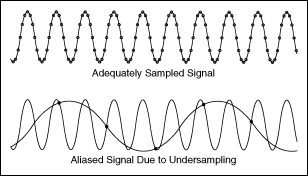
\includegraphics[scale = 2]{aliased_sig.png}
    \caption{Aliasing due to Undersampling. Available from: https://www.ni.com/docs/en-US/bundle/labview/page/lvanlsconcepts/aliasing.html}
    \label{fig:aliased}
\end{figure}
Hence, a natural question is whether we can use the sparsity assumption to reduce the number of measurements. To relate this to the preceding section, assume a linear measurement model, i.e. in Fourier space:
\begin{equation} \label{cs_lin}
    Ax = b,
\end{equation}
where $b \in \mathbb{C}^m$ is some vector that we measure, $A \in \mathbb{C}^{m \times N}$ is a discrete Fourier matrix. If we use a small number of measurements, that is, if $m < N$, then the system (\ref{cs_lin}) is under-determined and we generally cannot recover $x$. However, if we then assume that in our space $x$ is $s-$sparse, we can reduce our problem to basis pursuit, defined in the previous section. A scenario, where it is a priority to have as few samples as possible, is relevant in fields such as medical imaging, where obtaining samples is both costly to store and time-consuming. For example, patients (especially children and the elderly) cannot maintain the same posture for prolonged periods of time, especially if they are in pain.
%\section{Sparse Representations (Compression) (not sure about this section)}

A closely-related problem to that of compressed sensing is compression. The difference is - our primary goal now is to reduce the storage costs of a file, rather than being constrained by the number of samples. Signal compression involves two steps: \textbf{(I)} ``Coding" or representing a signal within a specified basis and \textbf{(II)} ``De-coding" or reconstructing the original signal using the basis and encoding coefficients. Commonly used bases are sinusoidal, such as a cosine basis (used in JPEG) or a wavelet basis (JPEG 2000). For example, for a signal $f$ and some orthonormal basis $\{\phi_m\}$, we first obtain the coefficients
\[a_n = \langle f,\phi_m \rangle,\]
where $\langle \cdot \rangle$ defines an inner product. This is followed by thresholding to create our $s-$sparse representation of largest coefficients. Basis pursuit can be used in the case where one has a basis in which they want to express a signal, but have no encoding-decoding process on-hand. An example of such a sparse representation can be seen in Figure \ref{fig:blurry_tiger}.

\subsection{Machine Learning}
Modern neural networks feature hundreds of thousands of weights, layers and connections. However, it has been shown that this is often unnecessary, as the network often has a large number of redundant weights and layers, which negligibly affect classification accuracy \cite{nn_toomuch}, while increasing the computational complexity of each forward pass. Furthermore, a large network may be trained to be too complex for the data at hand, i.e. overfitted \cite{nn_useful}. Most approaches to reducing these redundant parameters resort either to using some prior assumption about the specific network at hand, or to multiple training steps, both of which can present challenges. Such an approach by Han {\em et al.} first trains a network, then thresholds the small weights, thereafter retraining the remaining weights a second time \cite{nn_thresh}. However these chains of algorithms can be quite complex, involving both feature selection, training and pruning, and we are interested in more straightforward approaches that utilize sparse regularization to do all of this. One of these is proposed by Scardapane {\em et al.}, where sparse group lasso is used to enforce sparsity on batches of inputs corresponding to a single node \cite{nn_reg}.

\section{Tackling Sparse Problems}
Consider the LASSO optimization problem
\begin{equation} \label{xlasso}
\hat{x} = \argmin_{x} C(x,y) + \lambda \|x\|_1,
\end{equation}
where $C$ is smooth and convex. In the next sections we discuss approaches that were utilized to to tackle this kind of problem.

\subsection{Proximal-based methods}
We define the \textit{proximal operator}. Let $\phi : \mathbb{R}^n \xrightarrow[]{} \mathbb{R} \cup \{+\infty\}$ be given. Then $\mathrm{prox}_\phi: \mathbb{R}^n \xrightarrow[]{} \mathbb{R}^n$ is defined as
\begin{equation} \label{proximal}
    \mathrm{prox}_{\phi}(x) =\underset{z} \argmin \phi(z) + \frac{1}{2}\|z-x\|_2^2.
\end{equation}
A way to interpret this is that one wishes to find the minimum of $\phi$, without straying too far from $x$ \cite{proxalgs}. This mapping is well-defined \cite{fawzi2022lectures}. Furthermore, if we set $\mathcal{D}$ as some closed, convex set and choose $\phi$ as the indicator
\[\phi(x) = \begin{cases}
  0 \quad x \in \mathcal{D} \\
  +\infty \quad x \notin \mathcal{D}
\end{cases},\]
then $\mathrm{prox}_\phi$ reduces to the projection of $x$ onto $\mathcal{D}$. As such, the proximal mapping is a generalization of the projection operator. Suppose now that we have an optimization problem of the form
\begin{equation}
    \argmin_{x \in \mathbb{R}^n} {F(x, \lambda) \triangleq f(x) + g(x,\lambda)},
\end{equation}
where $f$ is smooth and convex and $g$ is nonsmooth convex. Analogously to the case when $g$ is differentiable, we can tackle this with subgradient methods. However, these are generally slower than gradient-based methods for smooth problems. Hence, we introduce the Proximal Gradient Descent method, also known as the Iterative Soft Thresholding Algorithm (or ISTA) \cite{daubechies2004iterative}. The update step for this algorithm reads
\begin{equation} \label{ISTA_step}
    x_{k+1} = \mathrm{prox}_{\gamma g}(x_k - \gamma \nabla f(x_k))
\end{equation}
for some step-size $\gamma$. To derive this, consider the quadratic approximation to $f(x)$ at $x_k$, with $\nabla^2 f \approx \frac{1}{\gamma}\mathrm{Id}$:
\[f_{app}(x) \approx f(x_k) + \nabla f(x_k)^\top (x-x_k) + \frac{1}{2\gamma} \|x-x_k\|_2^2.\]
Note that $f_{app}(x)$ is differentiable with respect to $x$, and by the first-order optimality condition, we can find the solution to 
\[\argmin_{x \in \mathbb{R}^n} f_{app}(x)\]
explicitly. This is
\[x = x_k - \frac{1}{\gamma} \nabla f(x_k),\]
which is the gradient descent step. Hence it is natural to consider
\begin{align*}
    x_{k+1} &= \argmin_{x \in \mathbb{R}^n} f_{app}(x) + g(x,\lambda) \\
    &= \argmin_{x \in \mathbb{R}^n} \frac{1}{2 \gamma} \|x - (x_k - \gamma \nabla f(x_k))\|_2^2 + g(x,\lambda) \\
    &= \mathrm{prox}_{\gamma g}(x_k - \gamma \nabla f(x_k)),
\end{align*}
which is exactly the update for proximal gradient descent. For various regularizers $g$, prox can be computed explicitly. For example, for $g = \|x\|_1$, we have $$\mathrm{prox}_{\gamma g}(x) = \mathrm{sign}(x) \max(|x|-\gamma,0).$$ This is illustrated in Figure \ref{fig:prox_lasso}.

\begin{figure}[h!]
    \centering
    \begin{tikzpicture}[
        declare function={
            func(\x)= (\x < -0.9) * (x+0.9)   +
                and(\x >= -0.9, \x < 0.9) * (0)     +
                (\x >= 0.9) * (x-0.9)
            ;
        }
    ]
        \begin{axis}[samples = 300,
            axis x line=middle, axis y line=middle,
            ymin=-5, ymax=5, ytick={-5,...,5}, ylabel=$x^j_{k+1}$,
            xmin=-5, xmax=5, xtick={-5,...,5}, xlabel=$x^j_{k} - \gamma \nabla f^j(x_k)$,
            ]
            \addplot [blue,thick] {func(x)};
            \addplot[mark=none] coordinates {(0.9,0)} node[pin=300:{$\gamma \lambda$}]{} ;
            \addplot[mark=none] coordinates {(-0.9,0)} node[pin=150:{$-\gamma \lambda$}]{} ;
        \end{axis}
    \end{tikzpicture} 
    \caption{The proximal step $\mathrm{prox}_{\gamma g}(x_k - \gamma \nabla f(x_k))$, with $g(x,\lambda) = \lambda \|x\|_1$.}
    \label{fig:prox_lasso}
\end{figure}

A nice feature of the proximal method is that it can also be formulated as a fixed-point iteration. Firstly, recall the definition of a subdifferential:
\begin{definition}[Subdifferential]
For a convex function $f : \mathbb{R}^n \to \mathbb{R} \cup \{+\infty\}$, the \emph{subdifferential} of $f$ at a point $x \in \mathbb{R}^n$ is defined as
\[
\partial f(x) = \bigl\{ v \in \mathbb{R}^n : f(y) \geq f(x) + v^\top (y - x) \;\; \text{for all } y \in \mathbb{R}^n \bigr\}.
\]
Each $v \in \partial f(x)$ is called a subgradient of $f$ at $x$. We say a function $f : \mathbb{R}^n \to \mathbb{R} \cup \{+\infty\}$ is subdifferentiable at a point $x$ if $\partial f(x) \neq \varnothing$.
\medskip

\noindent
\textbf{Remark.} If $f$ is differentiable at $x$, then the subdifferential reduces to the singleton
\[
\partial f(x) = \{ \nabla f(x) \}.
\]
\end{definition}
\begin{example}[Subdifferential of $|x|$]
Consider the absolute value function $f(x) = |x| $for $x \in \mathbb{R} $. Its subdifferential is
\[
\partial f(x) =
\begin{cases}
\{-1\}, & x < 0, \\[6pt]
[-1,1], & x = 0, \\[6pt]
\{1\}, & x > 0.
\end{cases}
\]
\end{example}
Additionally, we state some definitions that will be useful for this section.
\begin{definition}[Proper, lower semicontinuous, convex \cite{rockafellar1998variational}]
Let \(g : \mathbb{R}^n \to \mathbb{R} \cup \{+\infty\}\).  
We say that \(g\) is
\begin{itemize}
    \item \emph{proper} if \(g(x) > -\infty\) for all \(x \in \mathbb{R}^n\) and \(g \not\equiv +\infty\);
    \item \emph{lower semicontinuous} if
    \[
        \liminf_{y \to x} g(y) \;\geq\; g(x), \quad \text{ for all } x \in \mathbb{R}^n,
    \]
    or, alternatively, if the epigraph set
    $$
        \text { epi } f:=\left\{(x, \alpha) \in \mathbb{R}^n \times \mathbb{R} \mid \alpha \geq f(x)\right\}
    $$
    is closed on $\mathbb{R}^n \times \mathbb{R}$ \cite[Theorem 1.6]{rockafellar1998variational};
    \item \emph{convex} if
    \[
        g(\theta x + (1-\theta) y) \;\leq\; \theta g(x) + (1-\theta) g(y),
        \quad \text{ for all } x,y \in \mathbb{R}^n,\; \theta \in [0,1].
    \]
\end{itemize}
\end{definition}
Now, we state a useful result:
\begin{lemma}[Prox and Subdifferential, \cite{proxalgs}] \label{prox_subdif}
Let $g$ be a proper, lower semicontinuous, convex function. Assume also that $g$ is subdifferentiable on its domain, that is, $\partial g$ is nonempty on the domain. The proximal operator $\mathrm{prox}_{\gamma g}$ and the subdifferential $\partial g$ are related as follows. For $\gamma > 0$:
\begin{equation} \label{prox_partial}
    \mathrm{prox}_{\gamma g} = (I + \gamma \partial g)^{-1}.
\end{equation}
Note, that, just as $\partial g$ is a point-to-set mapping, that is, $\partial g$ takes each point $x \in \mathbf{dom}g$ to the set $\partial g (x)$, so are the operations on the right-hand side of (\ref{prox_partial}).
\end{lemma}
\begin{proof}
Suppose $z \in (I + \gamma \partial g)^{-1}(x)$, then
\begin{align*}
  x \in z + \gamma \partial g(z) &\iff \\
  0 \in \partial g(z) + \frac{1}{\gamma}(z-x) &\iff \\
  0 \in \partial_z \left(g(z) + \frac{1}{2\gamma} \|z-x\|_2^2 \right)
\end{align*}
By the first-order optimality condition, the above is necessary and sufficient for
\[z = \argmin_u \left(g(u) + \frac{1}{2\gamma}\|u-x\|_2^2 \right),\]
that is,
\[z = \mathrm{prox}_{\gamma g}(x).\]
\end{proof}
From the above, we see that $z \in (I + \gamma \partial g)^{-1}(x)$ if and only if $z = \mathrm{prox}_{\gamma g}(x).$ Furthermore, this tells us that the point-to-set operator $(I + \gamma \partial g)^{-1}$ is in fact a function. An immediate consequence is that minimizers of $f+g$ can be characterized as fixed points of the proximal gradient operator: a point $x^*$ solves $\min_x f(x)+g(x)$ if and only if
\[
x^* = \mathrm{prox}_{\gamma g}\!\left(x^* - \gamma \nabla f(x^*)\right).
\]
That is, minimizers are fixed points of the forward-backward operator. The proof follows directly from first-order optimality and Lemma~\ref{prox_subdif} (see \cite{proxalgs} for details).  
\begin{comment}
    \begin{lemma}[Fixed-Point of Forward-Backward]
Consider the problem
\[\min_x f(x) + g(x)\]
where $f: \mathbb{R}^n \xrightarrow[]{} \mathbb{R}$ and $g: \mathbb{R}^n \xrightarrow[]{} \mathbb{R} \cup \{+ \infty\}$ are proper lower semicontinuous convex and $f$ is differentiable. Let $\gamma > 0$. $x^*$ is a solution to the above problem if and only if it is a fixed point of
\[(I + \gamma \partial g)^{-1}(I - \gamma \nabla f).\]
Equivalently,
\[x^* = \mathrm{prox}_{\gamma g} \left(x^* - \gamma \nabla f(x^*)\right).\]
\end{lemma}
\begin{proof}
Let $\gamma>0$. $x^*$ minimizes $f+g$ if and only if
\begin{align*}
    0 \in \nabla f(x^*) + \partial g(x^*) &\iff \\
    %0 \in \nabla \gamma f(x^*) + \gamma \partial g(x^*) &\iff \\
    0 \in \nabla \gamma f(x^*) + x^* - x^* + \gamma \partial g(x^*) &\iff \\
    (I + \gamma \partial g)(x^*) \ni (I - \gamma \nabla f)(x^*)
\end{align*}
Now, by Lemma \ref{prox_subdif} and the fact that $(I + \gamma \partial g)^{-1}$ is single-valued, we have
\begin{align*}
x^* &= (I + \gamma \partial g)^{-1}(I - \gamma \nabla f)(x^*) \\
x^* &= \mathrm{prox}_{\gamma g} \left(x^* - \gamma \nabla f(x^*)\right).
\end{align*}
\end{proof}
Due to this result, proximal gradient descent is also known as \textit{forward-backward}: a forward step is taken with $(I - \gamma \nabla f)$, followed by a backward step $(I + \gamma \partial g)^{-1}$.
\end{comment}


The ISTA algorithm is stable and offers a cheap per-iteration cost, for regularizers such as $\ell_1$. However it also has a relatively slow $\mathcal{O}(1/k)$ convergence rate. As such, the related algorithm, FISTA (or Fast ISTA), was developed, where the proximal (or shrinkage) operator is applied not to the current iterate $x_k$, but to a linear combination of the current and previous iterates, $x_k$ and $x_{k-1}$. This algorithm was shown to have an improved $\mathcal{O}(1/k^2)$ convergence rate \cite{beck2009fista}.

\paragraph{Proximal splitting methods.} 
Beyond ISTA and its accelerated variant FISTA, a large family of first-order methods can be understood through the lens of proximal splitting. These methods exploit the structure of problems of the form
\[
    \min_{x \in \mathbb{R}^d} \; f(x) + g(x),
\]
where $f$ and $g$ are convex, possibly nonsmooth, functions. The idea is to use the proximal operators of $f$ and $g$ separately, avoiding the need to compute the proximal operator of their sum.

The Douglas--Rachford method was originally developed to solve problems of the form 
\[
    0 \in (A+B)(x),
\]
where $A$ and $B$ are monotone operators \cite{douglas1956numerical}. This abstract formulation unifies a wide range of problems: for instance, minimizing $f(x)+g(x)$ corresponds to the inclusion $0 \in \nabla f(x) + \partial g(x)$. The method iterates by alternating reflections with respect to the proximal maps of $A$ and $B$.

In addition, there is a large class of primal--dual proximal methods, such as the Chambolle--Pock algorithm \cite{chambolle2011first}, which explicitly update both primal and dual variables for problems with linear operators, for example of the form $\min_{x \in \mathbb{R}^d} \; g(x) + f(Kx)$. These methods generalize the proximal gradient framework to settings where dual variables naturally appear.

Together, these approaches illustrate the breadth of proximal algorithms: from simple gradient-based schemes such as ISTA and FISTA, to splitting methods like Douglas--Rachford, to fully primal--dual strategies.



\subsection{Hadamard Product Trick} \label{subsec: hada}
\begin{comment}
    \begin{figure}[h!]
    \centering
    \begin{tikzpicture}
        \begin{axis}[xmin=-4, xmax=4, ymin=-1,ymax=6, samples=100]
            \addplot[red, ultra thick, samples=250] {abs(x)};
            \addplot[blue] {(1/2)*(x*x/0.25 + 0.25)};
            \addplot[blue] {(1/2)*(x*x/0.5 + 0.5)};
            \addplot[blue] {(1/2)*(x*x/1 + 1)};
            \addplot[blue] {(1/2)*(x*x/2 + 2)};
        \end{axis}
    \end{tikzpicture}
    \caption{The function $|x|$, as the infimum of a family of smooth, convex quadratic functions of form $\frac{1}{2}\left(x^2z + \frac{1}{z} \right)$ (for various $z$).}
    \label{fig:my_label}
\end{figure}
\end{comment}


\begin{figure}[h!]
    \centering
    \begin{tikzpicture}
        \begin{axis}[xmin=-4, xmax=4, ymin=-1,ymax=6, samples=200,
                     axis lines=middle, xlabel={$x$}, ylabel={}]
            % |x|
            \addplot[red, ultra thick, samples=250] {abs(x)} node[pos=0.85, below] {};

            % Quadratics with different z
            \addplot[blue, domain=-4:4] {(1/2)*(x^2/0.25 + 0.25)} node[pos=0.8, below] {};
            \addplot[blue, domain=-4:4] {(1/2)*(x^2/0.5 + 0.5)}   node[pos=0.7, below] {};
            \addplot[blue, domain=-4:4] {(1/2)*(x^2/1 + 1)}       node[pos=0.6, below] {};
            \addplot[blue, domain=-4:4] {(1/2)*(x^2/2 + 2)}       node[pos=0.5, below] {};
        \end{axis}
    \end{tikzpicture}
    \caption{The function $|x|$ (in red), as the infimum of a family of convex quadratics $\tfrac12\big(z x^2 + \tfrac{1}{z}\big)$, with several shown for different $z>0$ (blue).}
    \label{fig:variational_abs}
\end{figure}
Consider the function $R(x) = |x|$. It admits the following quadratic variational representation:
$$|x| = \inf_{z>0}  \frac{1}{2}zx^2 + \frac{1}{2z}$$
To see this, fix $x$ and consider the function
$$f(z) = \frac{1}{2}zx^2 + \frac{1}{2z}.$$
Minimizing in $z$, we compute
$$f'(z) = \frac{1}{2}x^2 - \frac{1}{2z^2}.$$
Setting $f'(z) = 0$ gives the optimum $z^* = \frac{1}{|z|}$. Substituting the value back into $f$ gives
$$f(z^*) = |x|.$$ This simple example illustrates the principle that certain nonsmooth functions can be reformulated as quadratic variational problems. The following important theorem by Poon\cite{poon} states the general case.
\begin{theorem}[Quadratic Variational Form, \cite{poon}] \label{qvf_thm}
Let $R:\mathbb{R}^n \xrightarrow[]{} \mathbb{R}.$ Then the following are equivalent:
\begin{itemize}
    \item $R(\beta) = \phi(\beta \circ \beta)$, where $\phi$ is proper, concave and upper semi-continuous, with domain $R^d_+.$
    \item There exists a convex function $\psi$ for which $R(\beta) = \inf_{z \in \mathbb{R}^n_+} \frac{1}{2} \sum_{i=1}^n z_i \beta_i^2 + \psi(z).$
\end{itemize}
Furthermore, $\psi(z) = (-\phi)^* (-z/2)$ is defined via the convex conjugate $(-\phi)^*$ of $(-\phi)$. When $R$ is a norm, we have that, for $\psi(\eta) = \frac{1}{2} h(\frac{1}{\eta}),$
\[h(\eta) = \max_{R^*(\omega) \leq 1} \sum_i \omega_i \eta_i,\]
where $R^*$ is the dual norm of $R$.
\end{theorem}
In our case, for $R(\beta) = \|\beta\|_1$, we have that 
\[\phi(x) = \sum_i x^{\frac{1}{2}}\]
is a proper, concave and continuous function on $R^n_+$. By the above Theorem,
\begin{align*}
    \psi(z) &= (-\phi)^*(-z/2) \\
            &= \sup_{t \in \mathbb{R}^n} \left\{ \left\langle -\frac{z}{2},t \right\rangle - (-\phi)(t) \, \middle| \, t\in\mathbb{R}^n\right\} \\
            &= \sup_{t \in \mathbb{R}^n} \left\{ \left\langle -\frac{z}{2},t \right\rangle + \sum_i t^{\frac{1}{2}} \, \middle| \, t\in\mathbb{R}^n\right\}
\end{align*}
Using first-order optimality conditions, we can solve the above to get
\[\psi(z) = \frac{1}{2} \sum_i \frac{1}{z_i}.\]
Hence, by the equivalence result,
\begin{equation} \label{quad_form_l1}
    \|\beta\|_1 = \inf_{z \in \mathbb{R}^n_+} \frac{1}{2} \sum_{i=1}^n  \left( z_i \beta_i^2 + \frac{1}{z_i} \right).
\end{equation}
By change of variables $v_i = \frac{1}{\sqrt{z_i}}$, $u_i = \beta_i\sqrt{z_i}$, we finally obtain the equivalent formulation
\begin{equation} \label{uv_form_l1}
    \|\beta\|_1 = \inf_{\beta = u \circ v \in \mathbb{R}^n_+} \frac{1}{2} \sum_{i=1}^n  \left( u_i^2 + v_i^2 \right) = \inf_{\beta = u \circ v \in \mathbb{R}^n_+} \frac{1}{2} \left( \|u\|_2^2 + \|v\|_2^2 \right).
\end{equation}
As a result, the formulation (\ref{xlasso}) is equivalent to 
\begin{equation} \label{inprob_poon}
    \hat{u},\hat{v} = \underset{u,v \in \mathbb{R}^{n}} \argmin{C(u \odot v, \,y) + \frac \lambda 2 \left( \|u\|^2_2 + \lambda \|v\|^2_2 \right)},
\end{equation}
where $\odot$ denotes the Hadamard (or elementwise) product. The Hadamard product parametrization trades non-smoothness and convexity for smoothness and non-convexity. The formulation (\ref{inprob_poon}) can be tackled via first-order methods such as SGD, as well as variance reduction methods such as SVRG and SAGA \cite{defazio2014saga, johnson2013accelerating}, adaptive gradient methods, such as ADAM or ADAGRAD \cite{kingma2014adam, gupta2014training}, or via second-order methods such as (L-)BFGS \cite{liu1989limited}.

The quadratic variational reparametrization will be the central point of the work presented in Part \ref{part:Langevin}.
\begin{comment}
    \subsection{Other methods for non-smooth optimization}
There exist 
\begin{mdframed}[hidealllines=true,backgroundcolor=yellow!20]
    Talk about slow methods such as subgradient descent. Specialized methods, such as coordinate descent for $\ell_1$ and LARS.
\end{mdframed}
\end{comment}


\chapter{Background on Hyperparameter Optimization}
For a set of hyperparameters $\lambda \in \mathcal{D} \subset \mathbb{R}^r$, 
consider the optimization problem
\begin{equation} \label{regular}
    \min_{x \in \mathbb{R}^n} F(x,\lambda) \triangleq f(x) + g(x,\lambda),
\end{equation}
where $f : \mathbb{R}^n \to \mathbb{R}$ is smooth, and 
$g : \mathbb{R}^n \times \mathcal{D} \to \mathbb{R}$ may be smooth or nonsmooth. 
Various algorithms have been developed to solve problems of the form 
\eqref{regular}.

Recall from Eq.~\eqref{orig_lin} that we consider underdetermined linear 
inverse problems of the form $Ax=b$, with $m<N$. In practice, such problems 
are addressed via regularized formulations, where the parameter $\lambda$ 
controls the trade-off between data fidelity and structural priors. 
Choosing an appropriate value of $\lambda$ — for example, one that 
optimizes predictive performance or reconstruction accuracy — is 
generally problem-dependent and computationally nontrivial. 
This motivates the bilevel optimization framework studied in this chapter.


We are thus interested in solving problems of the form
\begin{align} 
&\min_{\lambda \in \mathcal{D} \subset \mathbb{R}^r} 
C(\hat{x}(\lambda), \lambda) \label{bilev1}\\
&\text{s.t. } 
\hat{x}(\lambda) = \argmin_{x \in \mathbb{R}^{n}} F(x, \lambda), 
\label{inprob}
\end{align}
where \eqref{bilev1} is referred to as the \emph{outer problem}, and 
\eqref{inprob} as the \emph{inner problem}. 
The function $C$ serves as a selection criterion for the hyperparameter 
$\lambda$, evaluated at the solution of the inner problem.

For example, $C$ may be chosen as a cross-validation loss: if a data matrix 
$A$ is split into $A_{\mathrm{train}}$ and $A_{\mathrm{test}}$, then
\[
C(\hat{x}(\lambda), \lambda)
= \|A_{\mathrm{test}} \hat{x}(\lambda) - b_{\mathrm{test}}\|_2^2.
\]


An alternative viewpoint is to reformulate the bilevel problem as a single-level constrained optimization problem, where the constraints are given by the first-order optimality conditions of the inner problem. However, depending on the inner problem, the number of constraints may be large and the feasible set may be non-convex. %Cite here
This brings us to the other approach - solving (\ref{bilev1}) directly with iterative algorithms. We began this report with motivations for studying sparse-regularized problems. However, ultimately, our goal is to investigate bilevel problems of the form (\ref{bilev1}). Below, we provide extensions of the previous sections with regards to this formulation.
\subsection{Hyperparameter Selection in Inverse Problems}
\begin{figure}[htp]
    \centering
    \begin{subfigure}[b]{0.3\textwidth}
        
\includegraphics[width=\linewidth]{IMG/tiger/tiger_orig.jpg}
        %\caption{Contact angle with various pseudo dosages}
        \label{fig:tiger_l1_gen0}
    \end{subfigure}
\hfil 
    \begin{subfigure}[b]{0.3\textwidth}
        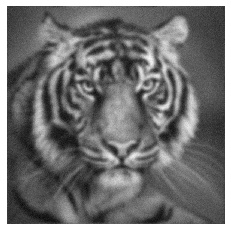
\includegraphics[width=\linewidth]{IMG/tiger/tiger_blur_noise_notext.jpg}
        %\caption{Contact angle with various pseudo dosages}
        \label{fig:tiger_l1_noise0}
    \end{subfigure}
\hfil
    \begin{subfigure}[b]{0.3\textwidth}
        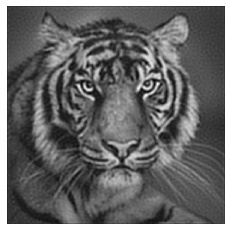
\includegraphics[width=\linewidth]{IMG/tiger/tiger_lasso_haar.jpg}
        %\caption{Contact angle with various pseudo dosages}
        \label{fig:tiger_l1_haar_opt}
    \end{subfigure}
    \caption{Example of an inverse problem: Benign image (left), noisy observation (center), sparse reconstruction in wavelet (Haar) basis (right). Refer to Figure \ref{fig:deblurry_tiger} for more examples of recovery.}\label{fig:blurry_tiger}
\end{figure}

Recall the imaging problem (\ref{lasso_gen}):
\begin{equation*}
    x^* = \argmin_x  \|Ax-b\|_2^2 + \lambda\|Dx\|_1.
\end{equation*}
Before we solve this problem, we need to consider the hyperparameter $\lambda > 0$, the weight of the regularization term. Note that as $\lambda \xrightarrow[]{} 0$, $x*$ approaches the solution of the non-regularized least squares problem, while as $\lambda \xrightarrow[]{} \infty$, the regularizer starts to dominate the solution. This is illustrated in Figure \ref{fig:deblurry_tiger}. We are interested in finding the optimal value of the hyperparameter, that is, a balance between sparsity of the solution, and its visual accuracy. To formalize this, we solve the bi-level problem
\begin{align} 
&\min _{\lambda \in \mathcal{D} \subset \mathbb{R}} L\left(\lambda \right) \triangleq C(\hat{x}(\lambda), \lambda) \label{bilev1_img}\\
&\text { s.t. } \hat{x}(\lambda) =\underset{x \in \mathbb{R}^{n}} \argmin \|Ax-b\|_2^2 + \lambda\|Dx\|_1 \label{inprob_img},
\end{align}
where $\mathcal{D}$ is non-empty, convex and compact and $C(\cdot,\lambda)$ is some smooth loss function. In compressed sensing, this could be the least-squares validation error. In denoising problems, SNR, or {\em signal-to-noise ratio} is often used \cite{gonzalez2008digital}:
\begin{equation}
    SNR(\hat{x}(\lambda), \lambda) = \frac{\|\hat{x}(\lambda) - x_0\|}{\|x_0\|},
\end{equation}
where $x_0$ denotes the clean image or signal. As this is generally not known in advance, this loss function is only used in an experimental setting. As the inner problem for inverse problems is often nonsmooth, such as in (\ref{inprob_img}), this creates a number of challenges when it comes to tackling such problems numerically. This will be further investigated in later sections.

\begin{example}[Dataset Distillation]
    An application of hyperparameter optimization in machine learning, that does not necessarily employ regularization is {\em dataset distillation}. The aim here is to condense the information within a training dataset $\mathbf{x}$ into a smaller, synthetic dataset $\mathbf{x}_{syn}$, such that training on this dataset would generalize to the validation and test sets. In the scope of hyperparameter optimization, the hyperparameters are the distilled images' pixels. The practical application of this is that the distilled images will contain useful information about the patterns that occur during the learning process \cite{lorraine2020optimizing}. To elaborate, let us formulate one approach, as per Cazenavette et al. \cite{cazenavette2022dataset}. When training a neural network, parametrized as $\theta$, our task is to find the parameters that minimize the empirical error, denoted by $\theta^*$, over the dataset $\mathbf{x} = \{x_i\}_{i=1}^N$:
\[\theta^* = \argmin_\theta \frac{1}{N} \sum_{i=1}^N \ell(x_i,\theta) \triangleq \argmin_\theta \ell(\mathbf{x},\theta),\]
where $\ell(x_i,\theta)$ denotes the error of the network at datapoint $x_i$ and $\ell(\mathbf{x},\theta)$ the average error. Now, a standard way to train a network is through gradient descent. At step $t$, we update our network parameters $\theta_t$ as follows:
\[\theta_{t+1} = \theta_t - \eta \nabla_{\theta_t} \ell(\mathbf{x}_t,\theta_t),\]
for some learning rate $\eta$ and minibatch $x_t$. However, for a large dataset, this generally takes many iterations to converge. The aim of Cazenavette et al. is to learn a small set $\mathbf{x}_{syn}$, so that the network performs well on the test set. Their approach is as follows: at every distillation step $t$ we train the network on the full real dataset $\mathbf{x}$, giving us a sequence of `expert' parameters $\theta_{t+1}, \theta_{t+2}, \hdots, \theta_{t+K}.$ We then initialize the `student' parameters as $\hat{\theta}_t = \theta_t$. This time, we do $M$ gradient descent iterations on our synthetic dataset $\mathbf{x}_{syn}$, with $M \ll K$, to get a sequence $\hat{\theta}_{t+1}, \hat{\theta}_{t+2}, \hdots, \hat{\theta}_{t+M}.$ At the end of the distillation step we compute the relative $L_2$ loss between the final 'student' and 'expert' parameters:
\[\mathcal{L}=\frac{\left\|\hat{\theta}_{t+M}-\theta_{t+K}^*\right\|_2^2}{\left\|\theta_t^*-\theta_{t+K}^*\right\|_2^2}.\]
Backpropagation is then used with $\mathcal{L}$ to update the set $\mathbf{x}_{syn}$ and the process is repeated. In the hyperparameter optimization framework, dataset distillation can also be formulated as follows: we can find the optimal synthetic dataset $\mathbf{x}_{syn}$ as
\begin{align}
    \mathbf{x}_{syn}^* &= \argmin_{\mathbf{x}_{syn}} \mathcal{L}_V(\mathbf{x}_{syn}, \theta^*(\mathbf{x}_{syn})), \text{ such that } \\
    \theta^*(\mathbf{x}_{syn}) &= \argmin_{\theta} \mathcal{L}_T(\mathbf{x}_{syn},\theta),
\end{align}
where $\theta$ denote network parameters, $\mathcal{L}_T$ and $\mathcal{L}_V$ are the training and validation losses, and $\theta^*(\mathbf{x}_{syn})$ are the best-response parameters to the current distilled images $\mathbf{x}_{syn}$. The validation set is populated by the labelled data, while the training set is populated by the distilled data \cite{lorraine2020optimizing}.
\end{example}

\begin{figure}[htp]
    \centering
    \begin{subfigure}[b]{0.3\textwidth}
        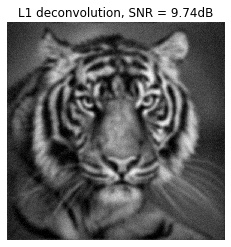
\includegraphics[width=\linewidth]{IMG/tiger_big/tiger_l1_gen.jpg}
        %\caption{Contact angle with various pseudo dosages}
        \label{fig:tiger_l1_gen}
    \end{subfigure}
\hfil 
    \begin{subfigure}[b]{0.3\textwidth}
        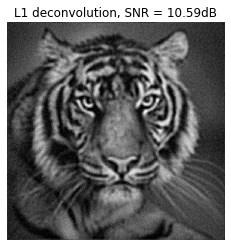
\includegraphics[width=\linewidth]{IMG/tiger_big/tiger_l1_opt.jpg}
        %\caption{Contact angle with various pseudo dosages}
        \label{fig:tiger_l1_opt}
    \end{subfigure}
\hfil
    \begin{subfigure}[b]{0.3\textwidth}
        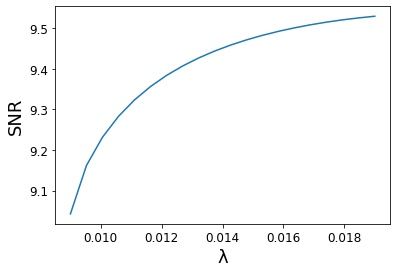
\includegraphics[width=\linewidth]{IMG/tiger_big/reg_path_l1.jpg}
        %\caption{Contact angle with various pseudo dosages}
        \label{fig:tiger_l1_path}
    \end{subfigure}

    \begin{subfigure}[b]{0.3\textwidth}
        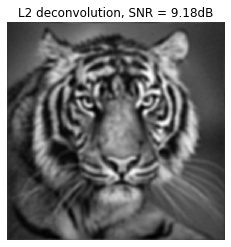
\includegraphics[width=\linewidth]{IMG/tiger_big/tiger_l2_gen.jpg}
        %\caption{Contact angle with various pseudo dosages}
        \label{fig:tiger_l2_gen}
    \end{subfigure}
\hfil 
    \begin{subfigure}[b]{0.3\textwidth}
        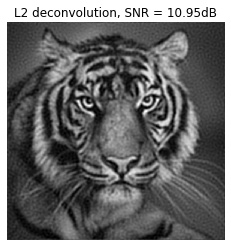
\includegraphics[width=\linewidth]{IMG/tiger_big/tiger_l2_opt.jpg}
        %\caption{Contact angle with various pseudo dosages}
        \label{fig:tiger_l2_opt}
    \end{subfigure}
\hfil
    \begin{subfigure}[b]{0.3\textwidth}
        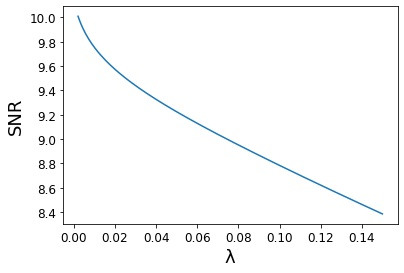
\includegraphics[width=\linewidth]{IMG/tiger_big/reg_path_l2.jpg}
        %\caption{Contact angle with various pseudo dosages}
        \label{fig:tiger_l2_path}
    \end{subfigure}
    
    \begin{subfigure}[b]{0.3\textwidth}
        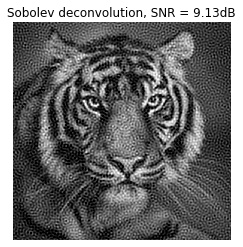
\includegraphics[width=\linewidth]{IMG/tiger_big/tiger_sob_gen.jpg}
        %\caption{Contact angle with various pseudo dosages}
        \label{fig:tiger_sob_gen}
    \end{subfigure}
\hfil 
    \begin{subfigure}[b]{0.31\textwidth}
        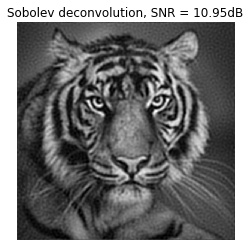
\includegraphics[width=\linewidth]{IMG/tiger_big/tiger_sob_opt.jpg}
        %\caption{Contact angle with various pseudo dosages}
        \label{fig:tiger_sob_opt}
    \end{subfigure}
\hfil
    \begin{subfigure}[b]{0.3\textwidth}
        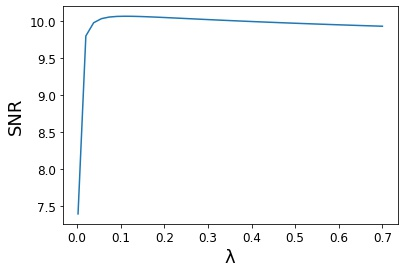
\includegraphics[width=\linewidth]{IMG/tiger_big/reg_path_sob.jpg}
        %\caption{Contact angle with various pseudo dosages}
        \label{fig:tiger_sob_path}
    \end{subfigure}

    \begin{subfigure}[b]{0.3\textwidth}
        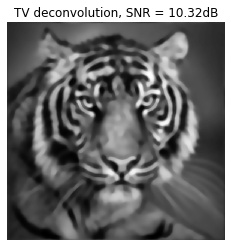
\includegraphics[width=\linewidth]{IMG/tiger_big/tiger_tv_gen.jpg}
        %\caption{Contact angle with various pseudo dosages}
        \label{fig:tiger_tv_gen}
    \end{subfigure}
\hfil 
    \begin{subfigure}[b]{0.3\textwidth}
        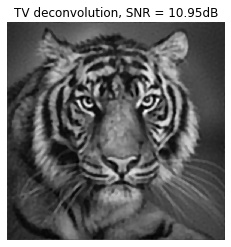
\includegraphics[width=\linewidth]{IMG/tiger_big/tiger_tv_opt.jpg}
        %\caption{Contact angle with various pseudo dosages}
        \label{fig:tiger_tv_opt}
    \end{subfigure}
\hfil
    \begin{subfigure}[b]{0.3\textwidth}
        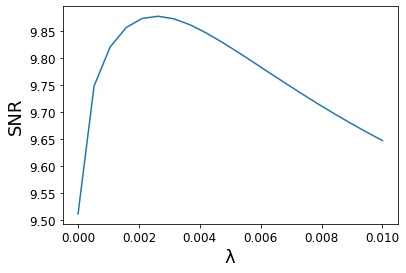
\includegraphics[width=\linewidth]{IMG/tiger_big/reg_path_tv.jpg}
        %\caption{Contact angle with various pseudo dosages}
        \label{fig:tiger_tv_path}
    \end{subfigure}
    \caption{Image deconvolution by regularization; Left: Arbitrary $\lambda$; Centre: Optimal $\lambda$ w.r.t. SNR; Right: Regularization path: SNR vs $\lambda$.}\label{fig:deblurry_tiger}
\end{figure}

\subsection{Existing Approaches}

\section{Hyperparameter Optimization with Smooth Inner Problem}
\label{section-hoag}
Recall the bi-level problem
\begin{align*} 
&\min _{\lambda \in \mathcal{D} \subset \mathbb{R}^r} L\left(\lambda \right) \triangleq C(\hat{x}(\lambda), \lambda)\\
&\text { s.t. } \hat{x}(\lambda) =\underset{x \in \mathbb{R}^{n}} \argmin {F(x, \lambda)},
\end{align*}
We consider the case, where both $C$ and $F$ are both smooth. 
\subsection{Existing Approaches}
Several notable approaches have been proposed to tackle bilevel optimization problems, particularly in settings where the lower-level problem must be solved numerically and exact hypergradients are unavailable. One classical approach is the HOAG algorithm proposed in~\cite{pedregosa2016hyperparameter}. HOAG computes hypergradients using the implicit function theorem, where the required inverse Hessian-vector product is approximated using conjugate gradients. It assumes that the error in this approximation is summable and uses a fixed step size for updating the upper-level parameters. While this approach can provide theoretical convergence guarantees, it may require unnecessarily tight tolerances on the inner solver, resulting in high computational cost. Stochastic bilevel optimization methods, such as those analyzed in~\cite{ghadimi2018approximation, hong2020twotimescale, ji2021bilevel}, have also gained popularity, especially in machine learning applications. These methods typically perform a fixed number of updates to the lower-level problem and update the upper-level variable using noisy or mini-batch hypergradients. While they scale well to large datasets, they often rely on specific assumptions such as stochastic smoothness or convexity, do not dynamically control accuracy or step size, and the larger number of hyperparameters in the form of batch sizes for the various stochastic subroutines can be difficult to tune. Another line of work explores fully first-order reformulations of bilevel problems as single-level constrained optimization problems via the introduction of a value-function constraint~\cite{ye2022bome}. These approaches avoid second-order information altogether but introduce penalty terms that require careful tuning. Moreover, the accuracy of lower-level approximations remains fixed, which can lead to inefficiencies in practice. Derivative-free methods such as DFO-LS~\cite{ehrhardt2021inexact} have also been adapted to bilevel learning. For example, DFO-LS applies trust-region derivative-free methods to optimize hyperparameters by solving the lower-level problem to a fixed tolerance and using the residual to guide the upper-level update. While promising in settings such as TV denoising, this method becomes less practical in high-dimensional settings due to poor scalability. Unlike prior methods (such as HOAG) that rely on static settings for gradient accuracy or step size, the MAID algorithm~\cite{salehi2024adaptively} dynamically adjusts both quantities based on computable error bounds and descent conditions. This adaptivity enables convergence with reduced computational effort and improves robustness to hyperparameter initialization, while demonstrating improved performance in tasks, such as logistic regression and TV denoising to that of HOAG or DFO-LS. A common flaw of algorithms for bilevel optimization is that they struggle in settings where the inner problem is ill-conditioned. We investigate this issue in Chapter \ref{chp: stoc_cond}. Another distinct line of work approaches hyperparameter learning from a statistical perspective, rather than as a bilevel optimization problem. For instance, Tan et al.~\cite{tan2024unsupervised} propose an unsupervised method for training convex neural regularizers by maximum marginal likelihood estimation. This approach estimates the parameters of the prior directly from noisy measurements, bypassing the need for ground-truth data or cross-validation. The framework scales to high-dimensional convex neural architectures, supported by convergence guarantees. This positions maximum likelihood--based approaches as a complementary alternative to classical bilevel hyperparameter optimization.

In the next section we will investigate the HOAG algorithm by Pedregosa, wherein we conduct gradient descent using an approximate hypergradient.

\begin{comment}
    \begin{mdframed}[hidealllines=true,backgroundcolor=yellow!20]
    Not sure if paper by Tan and Pereyra \cite{tan2024unsupervised} should be discussed in this section or elsewhere.
\end{mdframed}
\end{comment}




\subsection{Assumptions}
We will use a set of assumptions:
\begin{itemize}
    \item We assume that the first derivatives of $C$ and the second derivatives of $F$ are (globally) Lipschitz continuous.
    \item We assume that the Hessian $\nabla_{xx}^2 F$ is invertible at $(x(\lambda),\lambda)$ for all $\lambda \in \mathcal{D}$.
    \item We assume that the hyperparameter domain $\mathcal{D}$ is a convex non-empty and compact subset in $\mathbb{R}^r$.
\end{itemize}

%Mention here the chain rule that gives rise to all the below methods
%\subsection*{Algorithms}
\subsection{Prerequisites}
All of the algorithms presented in this section rely on two preliminary results. Firstly, we need to compute the gradient of the outer function $C$ with respect to a point $\lambda \in \mathcal{D}$. By definition of $\hat{x}(\lambda),$ we have by the optimality condition, that
\begin{equation} \label{opt_cond_smooth}
    \nabla_x F(\hat{x}(\lambda),\lambda) = 0.
\end{equation}
%% y is param, x is hyperparam
We can take the derivative of both sides. By chain rule, and implicit function theorem, we get
\begin{equation} \label{ift_opt}
    \nabla^2_{x\lambda} F(\hat{x}(\lambda),\lambda) + \nabla^2_{xx} F(\hat{x}(\lambda),\lambda) \nabla \hat{x}(\lambda) = 0,
\end{equation}
that is, 
%%
\[\nabla \hat{x}(\lambda) = -\left[ \nabla^2_{xx} F(\hat{x}(\lambda)) \right]^{-1}\nabla^2_{x \lambda} F(\hat{x}(\lambda)).\]
Also, by the chain rule we have
\[\nabla L(\lambda) = \nabla_\lambda C(\hat{x}(\lambda), \lambda) + \nabla \hat{x}(\lambda)^\top \nabla_x C(\hat{x}(\lambda), \lambda),\]
and so
\[\nabla C(\hat{x}(\lambda), \lambda) = \nabla_\lambda C(\hat{x}(\lambda)) - \nabla^2_{x \lambda} F(\hat{x}(\lambda))^\top \left[ \nabla^2_{xx} F(\hat{x}(\lambda)) \right]^{-\top} \nabla_x C(\hat{x}(\lambda), \lambda).\]
In the following algorithms $\nabla C(\hat{x}(\lambda), \lambda)$ will be computed in every outer-loop iteration. Of interest to us is the matvec product $\left[ \nabla^2_{xx} F(\hat{x}(\lambda)) \right]^{-\top} \nabla_x C(\hat{x}(\lambda)$. Computing and inverting the second derivative $\nabla^2_{xx} F$ is computationally expensive and so in later sections we consider approaches that numerically approximate either of these operations.
\subsection{Algorithm}
We can summarize the algorithm in four steps as follows:

\begin{algorithm}[H]
 \KwData{Input $x_0 \in \mathbb{R}^n$, $\lambda_0 \in \mathcal{D} \subset \mathbb{R}^r$, nonnegative sequence $\{\epsilon_k\}_{k\geq 0}$\;
 Tolerance $\epsilon_k = 0.1 \times k^{-n}$ for $n=2$ or $3$; or $\epsilon_k = 0.1 \times 0.9^k$\;}
 \For{$k = 0,1,\dots$}{
  Solve inner problem to tolerance $\epsilon_k$: find $x_k$ such that $\|\hat{x}(\lambda_k) - x_k\| \leq \epsilon_k$\;
  
  Solve linear system for $q_k$: 
  $\nabla^2_{xx} F(x_k,\lambda_k) q_k = \nabla_x C(x_k,\lambda_k)$ 
  up to tolerance $\epsilon_k$\;
  I.e., $\|\nabla^2_{xx} F(x_k,\lambda_k) q_k - \nabla_x C(x_k,\lambda_k)\| \leq \epsilon_k$\;
  
  Compute approximate gradient:
  $p_k = \nabla_\lambda C(x_k,\lambda_k) - \nabla^2_{x\lambda} F(x_k,\lambda_k)^\top q_k$\;
  
  Update hyperparameters:
  $\lambda_{k+1} = P_\mathcal{D} \left( \lambda_k - \frac{1}{L} p_k \right)$\;
  
  Projection operator:
  $P_\mathcal{D}(\alpha) = \arg\min_{\lambda \in \mathcal{D}} \|\alpha - \lambda\|^2$\;
 }
 \caption{HOAG Method}
 \label{alg:hoag}
\end{algorithm}
%Mention complexity-accuracy tradeoff for solving inner problem.

%\subsection*{BA - Ghadimi (NEED TO UPDATE NOTATION)}
%\begin{algorithm}[H]
 %\KwData{Input $x_0 \in \mathbb{R}^n, y_0 \in \mathbb{R}^m$, nonnegative sequences $\{\alpha_k\}_{k\geq 0},\{\beta_t\}_{t\geq 0}$, integer sequence $\{t_k\}_{k\geq 0}$}
 %\KwResult{Updated weights $w^{[l]}_{jk}$ and biases $b^{[l]}_j$}

 %\For{$k = 0,1,\hdots$}{
  %\For{$t = 0,1,\hdots,t_k - 1$ }{
    %Iterate inner loop steps
   % \[y_{t+1} = y_t - \beta_t \nabla_y g(x_k,y_t).\]
  %}
    %Set $\bar{y}_k = y_{t_k}$ and iterate one outer loop step
    %\[x_{k+1} = \argmin_{u \in X} \left \{\langle \bar{\nabla} f(x_k,\bar{y}_k), %u \rangle + \frac{1}{2 \alpha_k} \|u - x_k\|^2 \right \}\]
%    or, equivalently,
%    \[x_{k+1} = x_k - \alpha_k \bar{\nabla} f(x_k,\bar{y}_k)\]
    
% }
% \caption{Bilevel Approximation (BA) Method}
%\end{algorithm}
%To elaborate, here we have that
%\[\bar{\nabla} f(\bar{x},\bar{y}) = \nabla_x f(\bar{x},\bar{y}) - \nabla^2_{yx} g(\bar{x},\bar{y})^\top \left[ \nabla^2_{yy} g(\bar{x},\bar{y}) \right]^{-\top} \nabla_y f(\bar{x},\bar{y}).\]
Here we have to solve the inner problem to a high enough accuracy, so that the gradient approximation $p_k$ is close enough to $\nabla L$. Otherwise we might have divergence in the outer problem. Hence we have the complexity-accuracy trade-off between solving the inner problem and solving the outer problem. To be more precise, we present Pedregosa's main results about the convergence of HOAG.

\begin{theorem}[Bounded Gradient Error] \label{thm_appgrad_hoag}
In Algorithm \ref{alg:hoag}, for sufficiently large $k$, the gradient error is bounded as
\[\|\nabla L(\lambda_k) - p_k\| = \mathcal{O}(\epsilon_k).\]
\end{theorem}

This leads to the global convergence result.

\begin{remark} \label{hoag_mistake}
    Prior to November 2022, the convergence result in the paper\cite{pedregosa2016hyperparameter} claimed convergence of iterates $\lambda_k$ to their limit. However an error was found in the proof. A weaker result was proven, both by us and Pedregosa, regarding convergence of the gradient sequence $\nabla L(\lambda_k)$ to 0. We provide our result below, with proof in the appendix.
\end{remark}

\begin{theorem}[Global Convergence (Simplified)] \label{hoag_thm_simplified}
In Algorithm \ref{alg:hoag}, assume that the update
\[\lambda_{k+1} = P_\mathcal{D} \left( \lambda_k - \frac{1}{L}p_k \right),\]
is replaced by gradient descent with approximate gradient:
\[\lambda_{k+1} = \lambda_k - \frac{1}{L}p_k.\]
Assume also, that $\lambda_k \in \mathcal{D}$ for all $k>0$. If the sequence $\epsilon_k$ obeys
\[\sum_{i=1}^\infty \epsilon_i < \infty, \quad \epsilon_k > 0 \quad \text{ for all } k \geq 0,\]
\begin{comment}
    then the sequence $\lambda_k \xrightarrow[]{} \lambda^* \in \mathcal{D}.$ Furthermore, if $\lambda^*$ is in the interior of $\mathcal{D}$, then
\[\nabla L(\lambda^*) = 0.\]
\end{comment}
then $\lim_{k \xrightarrow[]{} \infty} \nabla L(\lambda_k) = 0.$
\end{theorem}

\section{On the Hessian}
%As mentioned previously, the complexity of computing and inverting the Hessian is costly. 
In the HOAG algorithm, every single gradient is computed directly. While this is feasible for first-order gradients, the complexity of second-order gradient calculations is $\mathcal{O}(n^3)$ (or $\mathcal{O}(mn^2)$). Furthermore, inverting the Hessian $\nabla^2_{yy} g$ has complexity $\mathcal{O}(n^3)$. In order to tackle this, a few approaches have been proposed. One is to use a quasi Newton (SR1) approximation to the Hessian.
\subsection{SR1 Update}
\label{section:sr1}
In optimization, one way of finding the minimum of a smooth, twice differentiable function $f: \mathbb{R}^n \xrightarrow[]{} \mathbb{R}$, is to use Newton's method \cite{nocedal2006numerical}. Recall a step of this iterative method. At a point $x_k + t$, for some small step $t \in \mathbb{R}^n$, consider the quadratic approximation of $f$:
\[f(x_k + t) \approx f(x_k) + \nabla f(x_k)^\top t + \frac{1}{2}t \nabla^2 f(x_k) t.\]
The gradient of the above, with respect to $t$, is
\[\nabla f(x_k + t) \approx \nabla f(x_k) + \nabla^2 f(x_k) t.\]
Assuming the Hessian $\nabla^2 f$ is invertible at $x_k$, the minimizer $t$ of the quadratic approximation is thus given by
\[t = -[\nabla^2 f(x_k)]^{-1} \nabla f(x_k).\]
Thus, the Newton method iteration can be written as 
\begin{equation} \label{newtonmethod}
    x_{k+1} = x_k - \gamma [\nabla^2 f(x_k)]^{-1} \nabla f(x_k),
\end{equation}
for some small $\gamma > 0$, chosen to satisfy the Wolfe conditions, which ensure that the step (\ref{newtonmethod}) results in a sufficient reduction in $f$ and $\nabla f$ \cite{nocedal2006numerical}. If $\nabla^2 f$ is Lipschitz continuous, then Newton's method has quadratic convergence\cite{nocedal2006numerical}. However, computing and inverting $\nabla^2 f$ may be costly, and so this motivates us to introduce quasi Newton methods. In short, these replace the Hessian inverse by a matrix $H \approx [\nabla^2 f(x_k)]^{-1}$ that is updated with each iteration. Recall the hypergradient calculation from HOAG:
\[\nabla C(\hat{x}(\lambda), \lambda) = \nabla_\lambda C(\hat{x}(\lambda)) - \nabla^2_{x \lambda} F(\hat{x}(\lambda))^\top \left[ \nabla^2_{xx} F(\hat{x}(\lambda)) \right]^{-\top} \nabla_x C(\hat{x}(\lambda), \lambda).\]
In the HOAG setting, quasi Newton methods have already been employed, replacing $\left[ \nabla^2_{xx} F(\hat{x}(\lambda)) \right]^{-1}$ with an approximation $H$, so that we have the approximate hypergradient
\[\nabla \tilde{C}(\hat{x}(\lambda), \lambda) = \nabla_\lambda C(\hat{x}(\lambda)) - \nabla^2_{x \lambda} F(\hat{x}(\lambda))^\top H^\top \nabla_x C(\hat{x}(\lambda), \lambda).\]
For example, in the paper by Ramzi et al. \cite{ramzi2022shine}, the proposed algorithm obtains the solution $\hat{x}(\lambda)$ for the inner problem and finds the the Hessian inverse  approximation $\left[ \nabla^2_{xx} F(\hat{x}(\lambda)) \right]^{-1}$ using $n$ steps of either the Broyden or BFGS method. It was shown theoretically, that the hypergradient $\nabla \tilde{C}(\hat{x}(\lambda), \lambda)$ converges superlinearly to $\nabla C(\hat{x}(\lambda), \lambda)$ as $n \xrightarrow[]{} \infty.$ Furthermore, it was shown empirically, that this approach converges faster than standard HOAG, when the inner problem was $\ell_2$-regularized logistic regression. Aside from BFGS and Broyden, there exists also the SR1, or Symmetric-Rank One method. Unlike the former, SR1 has a cheaper rank-1 update to the approximation $H$ and has shown, in practice, faster convergence to the true Hessian \cite{khalfan1993symmetric}. Motivated by this, we introduce the SR1 in the hyper-parameter optimization setting. Recall the optimality condition of the inner problem (\ref{opt_cond_smooth}):
\[\nabla_x F(\hat{x}(\lambda),\lambda) = 0.\]
In particular, we have, at step $k$:
\[\nabla_x F(\hat{x}(\lambda_k),\lambda_k) = 0.\]
Let us denote $\hat{x}(\lambda_{k}) \triangleq x_k$. The idea behind quasi Newton approximations is that information regarding the Hessian is maintained between iterates $x_k,x_{k+1}$ and their gradients $\nabla_x F(x_{k-1},\lambda_{k})$ and $\nabla_x F(x_{k},\lambda_{k}) = 0$. In particular, we have
\[\nabla_x F(x_{k-1},\lambda_{k}) = \nabla_x F(x_{k-1},\lambda_{k}) - \nabla_x F(\hat{x}(\lambda_k),\lambda_k)\]
Linearising, we finally get the \textit{secant condition}:
\begin{equation}\label{secant_sr1}
    \nabla_x F(x_{k-1},\lambda_{k}) - \nabla_x F(\hat{x}(\lambda_k),\lambda_k) = \nabla_{xx} F(x_{k},\lambda_{k})(x_{k-1} - x_k) + \mathcal{O}(\|x_{k-1} - x_k\|)
\end{equation}
We want to find an approximation $B$ of $\nabla_{xx} F(x_{k},\lambda_{k})^{-1}$, that also solves (\ref{secant_sr1}), or at the very least, such that
\[B = \min_{B} \|By_k - s_k\|,\]
where $y_k = \nabla_x F(x_{k-1},\lambda_{k}) - \nabla_x F(\hat{x}(\lambda_k),\lambda_k)$ and $s_k = x_{k-1} - x_k$. The general form of the SR1 approximation is as follows:
\begin{equation} \label{sr1_gen}
    B_{k+1} = B_{k} + \delta\sigma_k \sigma_k^\top.
\end{equation}
From the secant condition $B_k s_k = y_k$, (\ref{sr1_gen}) is satisfied if and only if \cite{nocedal2006numerical}
\[\sigma_k = \mathrm{sign}[s_k^t(y_k - B_k s_k)], \quad \delta = \pm |s_k^\top (y_k) - B_ks_k|^{-1/2}.\]
Thus, we have both a simple update rule for the Hessian,
\begin{equation} \label{sr1_upd}
    B_{k+1} = B_k + \frac{(y_k - B_ks_k)(y_k - B_ks_k)^\top}{(y_k - B_ks_k)^\top s_k},
\end{equation}
and, thanks to the Sherman-Morrison formula, a simple update for the Hessian inverse approximation $H_k$:
\begin{equation} \label{sr1_upd}
    H_{k+1} = H_k + \frac{(y_k - H_ks_k)(y_k - H_ks_k)^\top}{(y_k - H_ks_k)^\top s_k}.
\end{equation}
We propose an even simpler update rule:
\begin{equation} \label{sr1_poon}
    B_{k+1} = t_k \mathrm{Id} + \sigma_k \sigma_k^\top,
\end{equation}
that is, a Rank-1 modification of a diagonal matrix, where, necessarily,
$$t_k = \frac{\langle s_k, y_k \rangle}{\|y_k\|^2},$$
which is the solution of 
\[\argmin_t \|t_k \mathrm{Id} y_k - s_k\|.\]
This update is only applied if 
\[(y_k - B_ks_k)^\top s_k \neq 0,\]
which is not satisfied, if either $y_k = B_k s_k$ (in which case the secant condition is already satisfied by $B_{k+1} = B_k$), or if $(y_k - B_ks_k)$ and $s_k$ are orthogonal, in which case no solution for $\delta, \sigma$, satisfying (\ref{sr1_gen}) exists. Thus, in practice, for $B_0 = \gamma t_k \mathrm{Id}$, with $\gamma \in (0,1),$ we first check that:
\begin{equation} \label{orth_chck}
    \langle s_k - B_0z_k,z_k \rangle > 10^{-8} \|z_k\|\|\|s_k - B_0z_k\|,
\end{equation}
in which case we update
\[B_{k} = B_0 + \frac{(y_k - B_0s_k)(y_k - B_0s_k)^\top}{(y_k - B_0s_k)^\top s_k},\]
with the respective inverse update
\begin{equation*} \label{sr1_new_upd}
    H_{k} = H_0 + \frac{(y_k - H_0s_k)(y_k - H_0s_k)^\top}{(y_k - H_0s_k)^\top s_k},
\end{equation*}
where $H_0 = \frac{1}{\gamma t_k} \mathrm{Id}$. If (\ref{orth_chck}) does not hold, we set $B_{k} = B_0.$ This way, SR1 provides a cheap way to update the Hessian inverse between iterations, while keeping information change between the updates low.

\subsection{Neumann Series}
\label{subsec: neumann}
We have another result regarding matrix inversions: if $A$ is a positive-definite matrix, such that $\|A\| \leq 1$, then
\begin{equation} \label{neumann} 
    A^{-1} = \sum^{\infty}_{i=0} (I-A)^i.
\end{equation}
There are two consequences to this result. Firstly, we can use (\ref{neumann}) to approximately solve the linear system in Algorithm \ref{alg:hoag} by matrix-vector multiplications. Inverting an $m \times m$ Hessian would have a complexity of $\mathcal{O}(m^3)$, while leveraging an $L-$term Neumann series would have $\mathcal{O}(Lm^2)$, where we generally have $L<m$, especially for large datasets. However a more important consequence, is that we can derive a stochastic modification of the HOAG method. Recall the formulated problem 
\begin{align} 
&\min _{\lambda \in \mathcal{D} \subset \mathbb{R}^r} L\left(\lambda \right) \triangleq C(\hat{x}(\lambda), \lambda) \label{outer_hoag_neu}\\
&\text { s.t. } \hat{x}(\lambda) =\underset{x \in \mathbb{R}^{n}} \argmin {F(x, \lambda)}. \label{inner_hoag_neu}
\end{align}
The crux of this approach is that we can use (\ref{neumann}) to obtain a subroutine that finds a stochastic approximation to $[\nabla_{xx}^2 F]^{-1}$ and thus to $\nabla L$, matching these in expectation. The Hessian Inverse Approximation subroutine was first formulated by Ghadimi \& Wang \cite{ghadimi2018approximation}. Suppose, for a positive integer $b$, for a randomly chosen $p \in \{1,\cdots,b-1\}$, we have $p$ i.i.d. samples $\nabla^2_{xx} \tilde{F}_i$ of the Hessian  $\nabla^2_{xx} F$, so that $\mathbb{E}[\nabla^2_{xx} \tilde{F}_i(x,\lambda)] = \nabla^2_{xx} F(x,\lambda).$ Let $L_F$ denote the Lipschitz constant of $\nabla_x F$ (w.r.t. $x$). Then, if we denote
\begin{equation} \label{HIA}
    H_{xx} = \begin{cases}
        \frac{b}{L_F} \prod_{i=1}^p \left[\mathrm{Id} - \frac{1}{L_F}\nabla^2_{xx} \tilde{F}_i \right], \quad p \geq 1 \\
        \frac{b}{L_F} \mathrm{Id}, \quad p = 0,
    \end{cases}
\end{equation}
it can be shown, that
\[\mathbb{E}[H_{xx}] = \frac{1}{L_F} \sum_{i=0}^{b-1}\left[I-\frac{1}{L_F} \nabla^2_{xx} F(x,\lambda)\right]^i.\]
As a result, the Hessian Inverse Subroutine provides a biased estimate of $[\nabla_{xx}^2 F]^{-1}$, wherein the bias can be reduced by increasing the number of Hessian samples. However, Ghadimi did not provide any results on the variance of their approximation. Hence, a drawback of Ghadimi's neumann inversion subroutine, is that the variance of the resulting approximation forces us to use a diminishing stepsize in the outer loop to ensure convergence, and even in this case it is not guaranteed. As a result, a variant of (\ref{HIA}) was used by Ji, Yang \& Liang to develop the StocBio algorithm \cite{ji2021bilevel}. In short, StocBio is a double-loop algorithm. In the inner loop it finds a solution $x_k$ to the inner problem (\ref{inner_hoag_neu}) using stochastic gradient descent. We then construct, setting $\prod_{j=Q+1}^Q(\cdot) = I$,
\begin{equation} \label{HIA_StocBio}
    v_Q= \eta \sum_{q=-1}^{Q-1} \prod_{j=Q-q}^Q\left(I- \eta \nabla_y^2 \tilde{F}\left(x_k, \lambda_k ; \mathcal{B}_j\right)\right) \nabla_x \tilde{C}(x_k,\lambda_k,\mathcal{S}_C),
\end{equation}
where $\nabla_y^2 \tilde{F}\left(x_k, \lambda_k ; \mathcal{B}_j\right)$ are samples of the Hessian $\nabla_y^2 F \left(x_k, \lambda_k\right)$, taken from mutually independent sample sets $\{\mathcal{B}_j, j = 1, \hdots, Q\}$ and $\nabla_x \tilde{C}(x_k,\lambda_k,\mathcal{S}_C)$ is the randomly sampled gradient $\nabla_x C(x_k,\lambda_k)$. Here, as opposed to (\ref{HIA}), we approximate the inverse using independent sample sets. Note, that it is easy to see, that

\[\mathbb{E}[v_Q] = \eta \sum_{i=0}^{Q} \left[I - \eta\nabla_y^2 F \left(x_k, \lambda_k\right)\right]^i\nabla_x C(x_k,\lambda_k) \approx [\nabla_y^2 F \left(x_k, \lambda_k\right)]^{-1}\nabla_x C(x_k,\lambda_k).\]

Hence, we can use (\ref{HIA_StocBio}) to solve the system $\nabla_{xx}^2 F(x_k,\lambda_k)v = \nabla_x \tilde{C}(x_k,\lambda_k)$ (much like the second step in algorithm \ref{alg:hoag}) using only matrix-vector multiplication and low-sample approximations of the Hessian $\nabla_{xx}^2 F(x_k,\lambda_k)$. Finally, the approximate hypergradient is constructed:
\[\tilde{\nabla} L = \nabla_\lambda C(x_k,\lambda_k) - \nabla_{x \lambda}^2 F(x_k,\lambda_k)^\top v_Q.\]
Ji, Yang \& Liang have further developed two algorithms - MRBO and VRBO, building upon StocBio\cite{yang2021provably}. The former is a single loop algorithm, that uses momentum-based techniques to keep a running average of gradient estimations at each step, which are used to simultaneously update $x_k$ and $\lambda_k$. This method uses a decreasing stepsize for the updates. The latter is a double-loop algorithm that uses variance reduction techniques, similar to SVRG (Johnson \& Zhang \cite{johnson2013accelerating}). The outer loop is divided into epochs, while the inner loop, much like in the case of StocBio, solves the inner problem (\ref{inner_hoag_neu}), using the relevant gradients that are updated once per epoch with a relatively large batch of samples $\mathcal{S}_1$. Between the epochs the gradients are continuously updated using small batches of samples $\mathcal{S}_2$. To elaborate, the hypergradient $\nabla \tilde{L}$, when evaluated at the start of a new epoch, takes the form
\begin{equation} \label{VRBO_hyper}
    \begin{aligned}
&\widehat{\nabla} L\left(\lambda_k ; \mathcal{S}_1\right)=\frac{1}{S_1} \sum_{i=1}^{S_1}\left(\nabla_x C\left(x_k, \lambda_k ; \xi_i\right)\right. \\
&\left.\quad-\nabla_{x \lambda}^2 F\left(x_k, \lambda_k ; \zeta_i\right) \eta \sum_{q=-1}^{Q-1} \prod_{j=Q-q}^Q\left(I-\eta \nabla_x^2 F\left(x_k, \lambda_k ; \zeta_i^j\right)\right) \nabla_x C\left(x_k, \lambda_k ; \xi_i\right)\right),
\end{aligned}
\end{equation}
where all samples in $\mathcal{S}_1 = \left\{\zeta_i^j(j=1, \ldots, Q), \xi_i, \zeta_i, i=1, \ldots, S_1\right\}$ are independent. This method uses a constant stepsize. StocBio has a complexity of $\mathcal{O}(\epsilon^{-2})$ to reach such a point $\bar{\lambda}$, that $\|\nabla L(\bar{\lambda})\| \leq \epsilon.$ MRBO and VRBO, on the other hand, have a complexity of $\mathcal{O}(\epsilon^{-1.5})$ to achieve this. In fact, it was shown that these two algorithms outperform all of the existing stochastic bilevel optimization algorithms by a factor of $\mathcal{O}(\epsilon^{-0.5})$. Furthermore, all three of the stochastic algorithms demonstrated a faster convergence, as opposed to approximate implicit differentiation algorithms, such as HOAG (alg \ref{alg:hoag}).  
%Add sentence on how MRBO/VRBO or their analysis may be improved (discussed in future research section).
%Hence, the stochastic Hessian inverse subroutine provides a viable avenue for future research.
\newpage
\section{Hyperparameter Optimization with Non-Smooth Inner Problem}
\label{section-hoag_nonsmooth}
So far, we assumed the inner problem of bilevel optimization was smooth. In many practical settings, however, the inner objective includes non-smooth regularizers such as the $\ell_1$-norm in LASSO. This breaks the assumptions of classical implicit differentiation, since the inner solution map $\lambda \mapsto \hat{x}(\lambda)$ may fail to be differentiable everywhere. To be more specific, consider the following bilevel problem:
\begin{align} 
%&\min _{\lambda \in \mathbb{R}^r} L\left(\lambda \right) \triangleq \|A_{test}\hat{x}(\lambda) - b_{test}\|_2^2 \label{bilev_ns1}\\
&\min _{\lambda \in \mathbb{R}^r} L\left(\lambda \right) \triangleq \mathcal{C}(\hat{x}(\lambda),\lambda) \label{bilev_ns1}\\
&\text { s.t. } \hat{x}(\lambda) =\underset{x \in \mathbb{R}^{n}} \argmin {F(x,\lambda) \triangleq f(x) + \sum_{j=1}^\infty g_j(x,\lambda)} \label{inprob_ns},
\end{align}
where $g(x,\lambda) = \sum_{j=1}^\infty g_j(x,\lambda)$ is not differentiable. Several approaches have been proposed in the literature to address this issue. One line of work, due to Bertrand et al.~\cite{bertrand2022implicit}, develops a direct treatment of the nonsmooth setting using properties of proximal operators and active set identification. The key insight is that the proximal fixed-point mapping  
\[
x \mapsto \prox_{\gamma_j g_j}(x_j - \gamma_j \nabla f(x))
\]  
is differentiable at the optimum $\hat{x}$. Moreover, its gradient vanishes on the non-active set, which makes it possible to construct a Jacobian of the solution map despite nonsmoothness. This allows hypergradients to be computed via approximate linear system solves, leading to algorithms that resemble HOAG but explicitly account for sparsity structure.  

An alternative, proposed by Poon and Peyré~\cite{poon}, reparametrizes the nonsmooth problem into a smooth one, so that standard implicit differentiation applies directly. This smooth reformulation is the perspective adopted in this thesis.  


\subsection{Smooth reparametrization via Hadamard}
Consider the bilevel least squares problem
\begin{align} 
&\min _{\lambda \in \mathcal{D} \subset \mathbb{R}^r} L\left(\lambda \right) \triangleq \|A_{test} \hat{x}(\lambda) - b_{test}\|_2^2 \label{outprob_lsr}\\
&\text { s.t. } \hat{x} = \underset{x \in \mathbb{R}^{n}} \argmin{ \triangleq \frac{1}{2}\|Ax-b\|_2^2 + \lambda \|x\|_1}. \label{inprob_lsr}
\end{align}
Using the smooth reparametrization (\ref{inprob_poon}) from section \ref{subsec: hada} we can reformulate the above as
\begin{align} 
&\min _{\lambda \in \mathcal{D} \subset \mathbb{R}^r} L\left(\lambda \right) \triangleq \|A_{test} \left(\hat{u}(\lambda) \odot \hat{v}(\lambda) \right) - b_{test}\|_2^2 \label{outprob_poon_lsr}\\
&\text { s.t. } \hat{u},\hat{v} = \underset{u,v \in \mathbb{R}^{n}} \argmin{G(u,v)} \triangleq \frac{1}{2}\|A(u \odot v)-b\|_2^2 + \frac{\lambda}{2} \|u\|^2_2 + \frac{\lambda}{2} \|v\|^2_2. \label{inprob_poon_lsr}
\end{align}
We have turned the convex, non-smooth inner problem (\ref{inprob}) into a non-convex smooth optimization problem. Since both the inner and outer problems are now smooth, we can proceed as in HOAG\cite{pedregosa2016hyperparameter}. Note that, while $\hat{u} \odot \hat{v}$ is unique, $\hat{u}$ and $\hat{v}$ need not be, which may lead to continuity issues for (\ref{outprob_poon_lsr}). However, with additional restrictions, such as a positivity constraint $\hat{v} > 0$, this can be circumvented. For the inner problem, we can either do gradient descent on $u,v$, or further do a variable projection formulation. Consider the general inner problem:
\begin{equation} \label{inprob_ns}
    \hat{x}(\lambda) =\underset{x \in \mathbb{R}^{n}} \argmin  f(x) + \sum_{j=1}^\infty g_j(x,\lambda).
\end{equation}
By Theorem 2\cite{poon}, assuming $f$ is convex, proper and lower semi-continuous and that the regularizer $g(x) = \sum_{j=1}^\infty g_j(x,\lambda)$ in (\ref{inprob_ns}) has quadratic variational form, as in Theorem \ref{qvf_thm}, (\ref{inprob_ns}) is equivalent to
\begin{equation} \label{noncvx_varpro}
    \min_{v \in \mathbb{R}^n} f_{vp}(v) \triangleq \min_{u \in \mathbb{R}^n}{f(u \odot v) + \frac{\lambda}{2} \|u\|^2_2 + \frac{\lambda}{2} h(v \odot v)},
\end{equation}
with $h$, as in Theorem \ref{qvf_thm}. That is, in the case of LASSO, we have $h(v) = \sum_i v_i$, and so we can rewrite (\ref{inprob_poon}) as
\begin{equation} \label{noncvx_varpro_lasso}
    \min_{v \in \mathbb{R}^n} f_{vp} \triangleq \min_{u \in \mathbb{R}^n}{\frac{1}{2}\|A(u \odot v)-b\|_2^2 + \frac{\lambda}{2} \|u\|^2_2 + \frac{\lambda}{2} \|v\|_2^2}.
\end{equation}
%Note here, that Theorem 2 ensures that 
Furthermore, assuming $\lambda > 0$, we can explicitly write the gradient in closed form as
\begin{equation*}
    \nabla f_{vp}(v)=v +\frac{1}{\lambda} u \odot A^T\left( A(v \odot u) - b\right),
\end{equation*}
where $u = \argmin_{\tilde{u}} G(u,v). $ Now $\partial_u G(u,v) = 0$ and
\[\partial_{uu} G(u,v) = \frac{1}{\lambda} \mathrm{diag}(v)A^TA\mathrm{diag}(v) + \mathrm{Id}\]
has all positive eigenvalues $|\lambda_i|^2 + 1$, where $\lambda_i$ denotes the eigenvalue of $A\mathrm{diag}(v)$. Hence $\partial_{uu} G(u,v)$ is invertible. Thus, by implicit function theorem, we have that $u$ is a function of $v$ and
\begin{equation}\label{eq: fvphess}
    \nabla^2 f_{vp} = \partial_{vv} G(u,v) + \partial_{uv}G(u,v) \partial_v u = \partial_{vv} G(u,v) + \partial_{uv}G(u,v) [\partial_{uu}G(u,v)]^{-1}\partial_{vu}G(u,v),
\end{equation}
and so the Hessian $\nabla^2 f_{vp}$ is the Schur complement of 
$\nabla^2 G = 
\begin{pmatrix} 
\partial_{vv} G(u,v) & \partial_{uv} G(u,v) \\
\partial_{uv} G(u,v) & \partial_{uu} G(u,v)
\end{pmatrix}$
and as such, is better conditioned. Going by the result of Theorem 3\cite{poon}, even though the problem is non-convex, all of the saddle points of $f$ are either global minima or strict saddle points. This enables us to implement the variable projection formulation within a HOAG setting as:
\begin{align} 
&\min _{\lambda \in \mathcal{D} \subset \mathbb{R}^r} L\left(\lambda \right) \triangleq \|A_{test} \left(\hat{u}(\lambda) \odot \hat{v}(\lambda) \right) - b_{test}\|_2^2 \label{outprob_vp_poon}\\
&\text { s.t. } \hat{v}(\lambda) = \argmin_{v \in \mathbb{R}^n} f_{vp} \triangleq \min_{u \in \mathbb{R}^n}{\frac{1}{2}\|A(u \odot v)-b\|_2^2 + \frac{\lambda}{2} \|u\|^2_2 + \frac{\lambda}{2} \|v\|_2^2}, \label{inprob_vp_poon}
\end{align}
which we can tackle as in Algorithm \ref{alg:hoag}. 
\begin{comment}
    \begin{remark}
    It has been shown empirically, that, for tackling the problem
\begin{equation} \label{reg_prob_poon}
    \min_{x \in \mathbb{R}^n} \frac{1}{\lambda}L(Ax,b) + R(x),
\end{equation}
with the regularizer $R$ having quadratic variational form as per (\ref{qvf_thm}), solving the smooth reparametrization (\ref{noncvx_varpro}) with LBFGS-B is often superior (or comparable) to the current state-of-the-art methods for directly tackling (\ref{reg_prob_poon}). In particular, this approach is less sensitive to the choice of $\lambda$. Furthermore, by Theorem 2\cite{poon}, the gradient $\nabla f$ can be written in terms of the convex dual, with $L_y^*$ the convex dual of $L_y \triangleq L(\cdot,y)$, as
$$
\nabla f(v)=v \odot \partial h\left(v^2\right)-v \odot \left(\left\|X^{\top} \alpha\right\|^2\right) \quad \text { where } \quad \alpha \in \operatorname{argmax}_{\tilde{\alpha}}-L_y^*(\tilde{\alpha})-\frac{1}{2}\left\|v \odot \left(X^{\top} \tilde{\alpha}\right)\right\|_2^2,
$$
where $h$ is as in (\ref{noncvx_varpro}). We see that this does not depend on $\lambda$ and so this method allows for a smooth transition between $\lambda > 0$ and $\lambda = 0$, unlike other approaches (such as proximal algorithms on the non-parametrized problem).
\end{remark}
\end{comment}
\begin{remark}
    Empirically, when solving problems of the form
    \begin{equation} \label{reg_prob_poon_remark}
        \min_{x \in \mathbb{R}^n} \frac{1}{\lambda} L(Ax,b) + R(x),
    \end{equation}
    where the regularizer $R$ has a quadratic variational form as in (\ref{qvf_thm}), using the smooth reparametrization (\ref{noncvx_varpro}) with LBFGS-B often performs better — or at least comparably — to state-of-the-art methods that tackle (\ref{reg_prob_poon_remark}) directly. In particular, this approach is less sensitive to the choice of $\lambda$.

    Moreover, by Theorem 2\cite{poon}, the gradient $\nabla f$ can be expressed via the convex dual:
    \begin{equation*}
        \nabla f(v) = v \odot \partial h\left(v^2\right) - v \odot \Big\|X^\top \alpha\Big\|^2,
        \quad \text{where } \alpha \in \argmax_{\tilde{\alpha}} - L_y^*(\tilde{\alpha}) - \frac{1}{2}\Big\|v \odot (X^\top \tilde{\alpha})\Big\|_2^2,
    \end{equation*}
    and $L_y^*$ denotes the convex dual of $L_y(\cdot) \triangleq L(\cdot,y)$. 

    A key advantage of this representation is that $\nabla f$ does not depend on $\lambda$. This allows for a smoother transition between $\lambda > 0$ and $\lambda = 0$, which can be more stable in practice than directly applying proximal algorithms to the original non-parametrized problem.
\end{remark}



\begin{comment}
    \begin{mdframed}[hidealllines=true,backgroundcolor=yellow!20]
    Think of expanding this and add link to Stocbio/StocHOAG section.
\end{mdframed}
\end{comment}


\chapter{Background on Bayesian Sampling}
\section{Bayes' Theorem and Bayesian Sampling}
Bayes' theorem is a fundamental result in probability theory that describes how to update a prior belief in light of new evidence. It is given by:
\begin{equation}
p(\theta \mid \mathcal{D}) = \frac{p(\mathcal{D} \mid \theta) p(\theta)}{p(\mathcal{D})},
\end{equation}
where:
\begin{itemize}
\item $\theta$ represents the unknown parameters of a model;
\item $p(\theta)$ is the prior distribution, encoding our beliefs about $\theta$ before observing data;
\item $p(\mathcal{D} \mid \theta)$ is the likelihood function, describing the probability of the observed data $\mathcal{D}$ given $\theta$;
\item $p(\mathcal{D})$ is a scaling factor, representing the marginal likelihood or evidence, ensuring that $p(\theta \mid \mathcal{D})$ is a valid probability distribution;
\item $p(\theta \mid \mathcal{D})$ is the posterior distribution, which represents our updated beliefs about $\theta$ after observing the data.
\end{itemize}
Bayes' theorem provides a framework for statistical inference, enabling us to incorporate prior information into the analysis and systematically update our beliefs as new data becomes available. In many practical applications, the posterior distribution $p(\theta \mid \mathcal{D})$ is difficult to compute due to the complexity of the marginal likelihood $p(\mathcal{D})$, which requires integrating over all possible values of $\theta$:
\begin{equation}
p(\mathcal{D}) = \int p(\mathcal{D} \mid \theta) p(\theta) d\theta.
\end{equation}
Since this integral is difficult to compute exactly or even approximate, especially in high-dimensional problems, Bayesian sampling methods are employed to approximate the posterior distribution.
\section{Markov Chain Monte Carlo}
Markov Chain Monte Carlo (or MCMC) are a family of algorithms that construct a Markov chain whose stationary distribution is the posterior $p(\theta \mid \mathcal{D})$. A Markov chain is defined by a transition probability $P(\theta' | \theta)$, which describes the probability of moving from the current state $\theta$ to a new state $\theta'$, designed in a way so that the resulting Markov chain converges to $p(\theta \mid \mathcal{D})$ in distribution. Formally, we require that the target distribution is the invariant distribution \cite{andrieu2003introduction}:
\begin{equation*}
    p(\theta' \mid \mathcal{D}) = \sum_{\theta} P(\theta' | \theta)p(\theta \mid \mathcal{D}), \quad \text{ for all } \theta \in \mathbb{R}^d.
\end{equation*}
For guaranteed convergence to an invariant distribution $p(x)$ from any starting point (ergodicity) we require two conditions:
\begin{itemize}
    \item \textit{Irreducibility} - For any state there is a positive probability of reaching any other state, i.e. that we can reach any state in a finite number of steps (the transition graph is connected).
    \item \textit{Aperiodicity} - that there are no infinite cycles in the chain.
\end{itemize}
A sufficient condition for the ergodicity of a distribution $p(\theta' \mid \mathcal{D})$ is the detailed balance condition:
\begin{equation} \label{detailed_balance}
p\left(\theta^{(i)} \mid \mathcal{D}\right) P\left(\theta^{(i-1)} \mid \theta^{(i)}\right)=p\left(\theta^{(i-1)}\mid \mathcal{D}\right) P\left(\theta^{(i)} \mid \theta^{(i-1)}\right)
\end{equation}

MCMC methods are essential in Bayesian statistics as they enable inference in complex models where direct sampling is infeasible. Common MCMC methods include the Metropolis-Hastings algorithm and Gibbs sampling.%Common MCMC methods include:
%\begin{itemize}
%\item \textbf{Metropolis-Hastings Algorithm}: Proposes a new state $\theta'$ from a proposal distribution $q(\theta' \mid \theta^{(t)})$ and accepts it with probability:
%\begin{equation}
%A(\theta^{(t)}, \theta') = \min\left( 1, \frac{p(\theta') p(\mathcal{D} \mid \theta') q(\theta^{(t)} \mid \theta')}{p(\theta^{(t)}) p(\mathcal{D} \mid \theta^{(t)}) q(\theta' \mid \theta^{(t)})} \right).
%\end{equation}

%\end{itemize}

\section{The Gibbs Sampler}
Let $p(x_1, x_2, \dots, x_d)$ be a joint distribution with full conditionals
\[
p(x_i \mid x_{-i}) \quad \text{where } x_{-i} = (x_1, \dots, x_{i-1}, x_{i+1}, \dots, x_d).
\]
The Gibbs sampler generates a Markov chain $\{x^{(t)}\}_{t \geq 0}$ as follows:
\begin{enumerate}
    \item Initialize $x^{(0)} = (x_1^{(0)}, \dots, x_d^{(0)})$ arbitrarily.
    \item For $t = 1,2,\dots$ and $i = 1,\dots,d$, update sequentially
    \[
    x_i^{(t)} \sim p\!\left(x_i \,\middle|\, x_1^{(t)}, \dots, x_{i-1}^{(t)}, x_{i+1}^{(t-1)}, \dots, x_d^{(t-1)}\right).
    \]
\end{enumerate}
The resulting Markov chain has stationary distribution $p(x_1, \dots, x_d)$.
\begin{example}[Bivariate Gaussian]
Consider a bivariate normal distribution
\[
(x,y) \sim \mathcal{N}\!\left(
\begin{bmatrix} 0 \\ 0 \end{bmatrix},
\begin{bmatrix} 1 & \rho \\ \rho & 1 \end{bmatrix}
\right).
\]
The full conditional distributions are univariate Gaussians:
\[
x \mid y \;\sim\; \mathcal{N}(\rho y,\; 1 - \rho^2), 
\quad\quad
y \mid x \;\sim\; \mathcal{N}(\rho x,\; 1 - \rho^2).
\]
The Gibbs sampler alternates between sampling $x \mid y$ and $y \mid x$, producing a Markov chain whose stationary distribution is the target correlated Gaussian.
\end{example}
%A special case of Metropolis-Hastings where new samples are drawn from the full conditional distributions, cycling through each parameter sequentially:
\begin{comment}
Suppose you want to sample from a distribution over $d$ variables:
\begin{equation}
\theta_i^{(t+1)} \sim p(\theta_i \mid \theta_{-i}^{(t)}, \mathcal{D}).
\end{equation}
Gibbs sampling is particularly useful when the full conditionals are easy to sample from, which often occurs when working with conjugate priors. The method works as follows:
\begin{enumerate}
\item Initialize all parameters $\theta^{(0)}$.
\item For each iteration $t$, update each parameter $\theta_i$ sequentially by sampling from its conditional distribution given all other parameters:
\begin{align*}
    \theta_1^{(t+1)} &\sim p(\theta_1 \mid \theta_2^{(t)}, \dots, \theta_d^{(t)}, \mathcal{D}), \\
    \theta_2^{(t+1)} &\sim p(\theta_2 \mid \theta_1^{(t+1)}, \theta_3^{(t)}, \dots, \theta_d^{(t)}, \mathcal{D}), \\
    \vdots \\
    \theta_d^{(t+1)} &\sim p(\theta_d \mid \theta_1^{(t+1)}, \dots, \theta_{d-1}^{(t+1)}, \mathcal{D}).
\end{align*}

\item Repeat for a large number of iterations to approximate the posterior.
\end{enumerate}
Gibbs sampling is efficient when conditional distributions are easy to sample from.
\end{comment}



\chapter{Background on Stochastics}

\section{Introduction}
Stochastic processes play a fundamental role in modeling uncertainty. They provide a rigorous mathematical framework for describing systems that evolve randomly over time. In many applications, understanding randomness and its propagation is crucial for making predictions and optimizing decision-making strategies. In this chapter we provide background on stochastics needed to understand the contents of Part \ref{part:Langevin}.


%A stochastic process is a collection of random variables indexed by time $ \{X_t\}_{t \geq 0}$, where $X_t$ represents the state of the process at time $t$. 



\subsection{Brownian Motion and Measure-Theoretic Tools}
Brownian motion is a continuous-time stochastic process with independent and normally distributed increments. It serves as a fundamental building block in probability theory and has extensive applications in physics, finance, and engineering.

\begin{definition}[Brownian Motion on a Filtered Probability Space]
Let $(\Omega, \mathcal{F}, \{\mathcal{F}_t\}_{t \geq 0}, \mathbb{P})$ be a filtered probability space satisfying the usual conditions (completeness and right-continuity). A stochastic process $\{W_t\}_{t \geq 0}$ is called a \emph{standard Brownian motion} (or \emph{Wiener process}) with respect to this filtration if:

\begin{enumerate}
    \item $W_0 = 0$, $\mathbb{P}$-almost surely.
    \item $W_t$ is $\mathcal{F}_t$-adapted.
    \item For all $0 \leq s < t$, the increment $W_t - W_s \sim \mathcal{N}(0, t-s)$ (Gaussian increments).
    \item The process has independent increments: for all $0 \le t_0 < t_1 < \dots < t_n$, the random variables $W_{t_1} - W_{t_0}, \dots, W_{t_n} - W_{t_{n-1}}$ are independent.
    \item The sample paths $t \mapsto W_t(\omega)$ are almost surely continuous.
\end{enumerate}
\end{definition}

Brownian motion is a martingale, meaning that its expected future value given past observations remains equal to its current value:
\begin{equation}
    \mathbb{E}[B_t \mid \mathcal{F}_s] = B_s, \quad \text{for } s \leq t.
\end{equation}
This property is crucial in stochastic integration and financial mathematics.

\begin{definition}[Radon--Nikodym Theorem]
Let $(\Omega, \mathcal{F})$ be a measurable space and let $\mathbb{Q}$ and $\mathbb{P}$ be $\sigma$-finite measures on $(\Omega, \mathcal{F})$, with $\mathbb{Q} \ll \mathbb{P}$ (i.e., $\mathbb{Q}$ is absolutely continuous with respect to $\mathbb{P}$). Then there exists a unique (up to $\mathbb{P}$-almost everywhere equivalence) measurable function $Z : \Omega \to [0,\infty)$, called the Radon--Nikodym derivative, such that for every measurable set $A \in \mathcal{F}$,
\[
\mathbb{Q}(A) = \int_A Z \, d\mathbb{P}.
\]
We write
\[
Z = \frac{d\mathbb{Q}}{d\mathbb{P}}.
\]
\end{definition}
In the context of stochastic processes, we often define a new probability measure $\mathbb{Q}$ on a filtered probability space such that the law of a process (e.g., a Brownian motion) under $\mathbb{Q}$ differs from its law under $\mathbb{P}$. The Radon--Nikodym derivative then appears as a density process, typically of the form
\[
\frac{d\mathbb{Q}}{d\mathbb{P}} \bigg|_{\mathcal{F}_t} = M_t,
\]
where $(M_t)_{t \geq 0}$ is a positive martingale like the exponential martingale discussed above. This is the key object in Girsanov’s theorem, allowing us to shift the drift of Brownian motion.

\begin{definition}[Exponential Martingale]
Let $(\Omega, \mathcal{F}, (\mathcal{F}_t)_{t \geq 0}, \mathbb{P})$ be a filtered probability space and let $(B_t)_{t \geq 0}$ be a standard Brownian motion adapted to $(\mathcal{F}_t)$. Suppose $X = (X_t)_{t \geq 0}$ is an $(\mathcal{F}_t)$-adapted process such that
\[
\mathbb{E} \left[ \exp\left( \frac{1}{2} \int_0^T X_s^2 \, ds \right) \right] < \infty.
\]
Then the process
\[
M_t := \exp\left( \int_0^t X_s \, dB_s - \frac{1}{2} \int_0^t X_s^2 \, ds \right)
\]
is called an \emph{exponential martingale}.

\medskip
Under appropriate conditions, $M_t$ is a true martingale, and plays the role of a Radon--Nikodym derivative for a change of measure that modifies the drift of $B_t$.
\end{definition}

\begin{proposition}[Novikov’s Condition] \label{nov_cond}
Let $X = (X_t)_{t \geq 0}$ be an $(\mathcal{F}_t)$-adapted process. If
\[
\mathbb{E} \left[ \exp\left( \frac{1}{2} \int_0^T X_s^2 \, ds \right) \right] < \infty,
\]
then the exponential process
\[
M_t := \exp\left( \int_0^t X_s \, dB_s - \frac{1}{2} \int_0^t X_s^2 \, ds \right)
\]
is a true martingale on $[0,T]$.
\end{proposition}
\medskip

This sufficient condition ensures that the stochastic exponential does not grow too rapidly. It is often invoked in the application of Girsanov's theorem to justify a change of measure and interpret the modified process as a Brownian motion under the new probability measure.

\begin{theorem}[Girsanov's Theorem, \texorpdfstring{\cite[Theorem~5.1]{Karatzas1991-xr}}{}]
Let $$X=\left\{X_t=\left(X_t^{(1)}, \ldots, X_t^{(d)}\right), \mathcal{F}_t ; 0 \leq t<\infty\right\}$$ be a vector of measurable adapted processes satisfying
$$
P\left[\int_0^T\left(X_t^{(i)}\right)^2 d t<\infty\right]=1 ; \quad 1 \leq i \leq d, \quad 0 \leq T<\infty.
$$
Assume that $Z(X)$ defined by 
$$
Z_t(X) \triangleq \exp \left[\sum_{i=1}^d \int_0^t X_s^{(i)} d W_s^{(i)}-\frac{1}{2} \int_0^t\left\|X_s\right\|^2 d s\right]
$$
is a martingale (satisfied by \cite[Corollary 5.13 of Novikov Condition]{Karatzas1991-xr}). Define a process $\tilde{W}=\left\{\tilde{W}_t=\left(\tilde{W}_t^{(1)}, \ldots\right.\right.$, $\left.\left.\tilde{W}_t^{(d)}\right), \tilde{\mathcal{F}}_t ; 0 \leq t<\infty\right\}$ by

$$
\tilde{W}_t^{(i)} \triangleq W_t^{(i)}-\int_0^t X_s^{(i)} d s ; \quad 1 \leq i \leq d, \quad 0 \leq t<\infty
$$


For each fixed $T \in[0, \infty)$, the process $\left\{\tilde{W}_t, \tilde{\mathcal{F}}_t ; 0 \leq t \leq T\right\}$ is a d-dimensional Brownian motion on ( $\Omega, \mathcal{F}_T, \widetilde{P}_T$ ).
\end{theorem}

\begin{comment}
    \subsection{Applications}
Brownian motion is used in various fields, including:
\begin{itemize}
    \item \textbf{Physics}: Describing the random motion of particles suspended in a fluid, as first observed by Robert Brown.
    \item \textbf{Finance}: Modeling stock prices and interest rates in the Black-Scholes framework.
    \item \textbf{Engineering}: Noise modeling in signal processing and control systems.
\end{itemize}
\end{comment}




\section{SDEs and It\^{o} Calculus}
Stochastic Differential Equations (SDEs) extend ordinary differential equations by incorporating stochastic processes, typically driven by Brownian motion. These equations model systems subject to random fluctuations.

A general SDE is expressed as:
\begin{equation} \label{sde_eqn_diff}
    dX_t = \mu(X_t, t) dt + \sigma(X_t, t) dB_t, \quad X(0) = x,
\end{equation}
for $X \in \mathbb{R}^d$, $t \in [0,T]$, where $\mu(X_t, t): \mathbb{R}^d \times [0,1] \xrightarrow[]{} \mathbb{R}^d$ and $\sigma(X_t, t): \mathbb{R}^d \times [0,1] \xrightarrow[]{} \mathbb{R}^{d \times n}$ are measurable functions that represent the drift and diffusion terms and $B_t$ is a vector of $n$ independent Brownian motions. (\ref{sde_eqn_diff}) is the differential form of the stochastic integral equation
\begin{equation} \label{sde_eqn_int}
    X_t = x + \int_0^t \mu(X_s, s) ds + \int_0^t\sigma(X_s, s) dB(s).
\end{equation}
It\^{o} calculus provides the framework for analyzing stochastic integrals and differential equations. The It\^{o} integral of a process $f(t)$ with respect to Brownian motion $B_t$ is defined as:
\begin{equation} \label{ito_int}
    \int_0^t f(s) dB_s = \lim_{K \xrightarrow[]{} \infty} \sum_{k=0}^{K-1} f(t_k) (B(t_{k+1}) - B(t_k)),
\end{equation}
where $f$ is an adapted process with respect to the filtration $\{\mathcal{F}_t\}$, generated by the Brownian motion $B_t$. Assuming $f$ is square-integrable, the It\^{o} Integral satisfies the It\^{o} isometry \cite{pavliotis_book}:
\begin{equation} \label{ito_isometry}
    \mathbb{E} \left[ \int_0^T f(t) dB(t)\right]^2 = \int_0^T \mathbb{E}|f(t)|^2 dt.
\end{equation}
Furthermore, the It\^{o} Integral is a martingale, so that 
\begin{equation} \label{ito_martin_mean}
    \mathbb{E} \int_0^t f(s) d B(s)=0
\end{equation}
and
\begin{equation} \label{ito_martin}
\mathbb{E}\left[\int_0^t f(\ell) d B(\ell) \mid \mathcal{F}_s\right]=\int_0^s f(\ell) d B(\ell) \quad \text{ for all } t \geqslant s,
\end{equation}
where $\mathcal{F}_s$ denotes the filtration generated by $B(s)$. In stochastic calculus differentiation is redefined via It\^{o}'s lemma:
\begin{equation} \label{ito_lem}
    dF(X_t) = \frac{\partial F}{\partial x} dX_t + \frac{1}{2} \frac{\partial^2 F}{\partial x^2} (dX_t)^2.
\end{equation}
With regards to SDE \ref{sde_eqn_diff}, we can expand the above to obtain a more explicit form. For twice differentiable $F$,
\begin{equation} \label{ito_lem_exp}
    dF(X_t) = \left\{(\nabla_x F)^T \mu_t(X_t) + \frac{1}{2} [\sigma_t(X_t)\sigma_t(X_t)^T (H_x F) ] \right\} \,dt + (\nabla_x F)^T \sigma_t(X_t) dB_t,
\end{equation}
where $\nabla_x F$ and $H_x F$ are the Jacobian and Hessians of $F$ \cite{pavliotis_book}.

\subsection{Examples of SDEs}
\begin{itemize}
    \item \textbf{Geometric Brownian Motion}: Used to model stock prices in finance.
    \begin{equation}
        dS_t = \mu S_t dt + \sigma S_t dB_t.
    \end{equation}
    \item \textbf{Ornstein-Uhlenbeck Process}: Models mean-reverting behavior in physics and finance.
    \begin{equation}
        dX_t = \theta (\mu - X_t) dt + \sigma dB_t.
    \end{equation}
\end{itemize}

\section{Generators and Kolmogorov Equations}
Consider the SDE
\begin{equation} \label{aut_sde}
    dX_t = \mu(X_t) dt + \sigma(X_t) dB_t, \quad X(0) = x.
\end{equation}
Recall, that, given a sufficiently smooth test function $F: \mathbb{R}^d \xrightarrow[]{} \mathbb{R}$, using It\^{o}'s Lemma we can derive
\begin{equation} \label{ito_lem_gen}
    dF(X_t) = \mathcal{L}F dt + (\nabla_x F)^T \sigma(X_t) dB_t,
\end{equation}
with
\begin{equation} \label{generator_explicit}
    \mathcal{L} = \mu(x) \cdot \nabla + \frac{1}{2}\sigma(x)\sigma(x)^T : \nabla^2
\end{equation}
 where $\nabla$ and $\nabla^2$ denote the Jacobian and Hessian operators, respectively, and $:$ denotes the Frobenius inner product. Integrating and taking expectations, we can show that
\begin{align}
    \mathbb{E}^x\left[F(X_t) - F(X(0))\right] &= \mathbb{E}^x\left[\int_0^t \mathcal{L}F ds + \int_0^t (\nabla_x F)^T \sigma(X_t) dB_s \right] \label{generator_int} \\
    &= \mathbb{E}^x\left[\int_0^t \mathcal{L}F ds \right] \label{generator_martin},
\end{align}
where (\ref{generator_martin}) follows from the martingale property (\ref{ito_martin}). Finally, by continuity of $F$, we obtain
\begin{equation} \label{eqn_generator}
    \mathcal{L}F(x) = \lim_{t \xrightarrow[]{} 0}\frac{\mathbb{E}\left[F(X_t) | X(0) = x \right]- F(x)}{t}.
\end{equation}
That is, $\mathcal{L}$ is the generator of \ref{aut_sde}. Let $\phi = \mathbb{E}\left[F(X_t) | X(0) = x \right]$. From (\ref{eqn_generator}) we can directly compute the backward Kolmogorov Equation,
\begin{equation} \label{eqn_BKE}
    \partial_t \phi = \mathcal{L} \phi, \quad \phi(x,0) = F(x).
\end{equation}
which describes the time evolution of expectations of functionals with respect to random variable $X_t$. Also of interest to us is the $L^2$ adjoint of the generator, also referred to as the Fokker-Planck operator and denoted $\mathcal{L}^{\dagger}$. Given test functions $f,g$, this operator satisfies
\begin{equation}
    \int (\mathcal{L}f)(x)g(x) dx = \int f(x)(\mathcal{L}^{\dagger}g)(x) dx
\end{equation}
and, using integration by parts, can be explicitly found from (\ref{generator_explicit}) as
\begin{equation} \label{gen_dag_explicit}
    \mathcal{L}^{\dagger} = -\mathrm{div}(b\cdot) + \frac{1}{2} \nabla^2:(\sigma \sigma^T)
\end{equation}
The importance of the Fokker-Planck operator to SDE theory lies in the fact that it describes the time evolution of the density function of associated stochastic differential equation. With regards to SDE (\ref{aut_sde}), assume the random variable $X_t$ at time $t$ has density $\psi$ with respect to Lebesgue measure - $X_t \sim \psi(t,x) dx$, with $\psi(0,x) = \psi_0(x).$ Then $\psi$ satisfies the forward Kolmogorov Equation (also known as the Fokker-Planck equation):
\begin{equation} \label{eqn_FP}
    \partial_t \psi = \mathcal{L}^\dagger \psi, \quad \psi(0) = \psi_0.
\end{equation}
The steady-state behavior of a stochastic process is described by invariant distributions. That is, we say a distribution $P(t,X,\cdot)$ is invariant at time $t$, if it doesn't change with respect to $t$. If a stochastic process has a unique invariant measure, then it is known as an \textit{ergodic} measure. In later sections, one of our foci will be the identification of a system of SDEs with a target invariant distribution. With this in mind, and by (\ref{eqn_FP}), the distribution $\rho$ is an invariant distribution of the stochastic process, associated with operator $\mathcal{L}^{\dagger}$ if and only if
\begin{equation}\label{eqn_FP_inv}
    \mathcal{L}^{\dagger} \rho = 0.
\end{equation}


\begin{example}[Overdamped Langevin Dynamics]
Consider the case of overdamped Langevin dynamics:
\[dx_t = -\nabla V(x_t) dt + \sqrt{2\beta^{-1}}dWt,\]
with Brownian motion $W$, $\beta  > 0$.
    Forward equation is
    $$
\mathcal{L}^{\dagger} \psi=\operatorname{div}(\nabla V \psi)+\frac{1}{\beta} \Delta \psi=\frac{1}{\beta} \operatorname{div}\left[\mathrm{e}^{-\beta V} \nabla\left(\mathrm{e}^{\beta V} \psi\right)\right] .
$$
    We can easily check $\nu \sim \exp{(-\beta V)}$ is a stationary distribution:
    \[\mathcal{L}^{\dagger} \nu = \frac{1}{\beta} \operatorname{div}\left[\mathrm{e}^{-\beta V} \nabla\left(\mathrm{e}^{\beta V} \nu\right)\right] = 0.\]
\end{example}


\section{Convergence of SDEs}

Consider the overdamped Langevin dynamics given by the stochastic differential equation:
\begin{equation}
dx_t = -\nabla V(x_t) dt + \sqrt{\frac{2}{\beta}} dW_t.
\end{equation}
The associated Fokker-Planck equation, which governs the evolution of the probability density $\psi_t$ of $x_t$, is given by:
\begin{equation}
\frac{\partial \psi}{\partial t} = \mathcal{L}^{\dagger} \psi,
\end{equation}
where the backward Kolmogorov operator $\mathcal{L}$ and its adjoint $\mathcal{L}^{\dagger}$ in $L^2(\mathbb{R}^d)$ satisfy the relation:
\begin{equation}
\mathcal{L}^{\dagger} \psi = \operatorname{div} (\nabla V \psi) + \frac{1}{\beta} \Delta \psi.
\end{equation}
It is straightforward to verify that the measure $\nu$ with density:
\begin{equation}
\nu(dx) \propto e^{-\beta V(x)} dx
\end{equation}
is invariant under the dynamics, meaning that if $x_t \sim \nu$, then $x_{t+s} \sim \nu$ for all $s \geq 0$. This raises the fundamental question:

\begin{center}
\textbf{Does $\psi_t$ converge to $\nu$? If so, how fast?}
\end{center}

To analyze this, we consider a transformation of the density function. Define $f = \psi e^{\beta V}$, which satisfies the evolution equation:
\begin{equation}
\frac{\partial f}{\partial t} = \mathcal{L} f,
\end{equation}
where the integral constraint:
\begin{equation} \label{FP_reform}
\int_{\mathcal{D}} f e^{-\beta V} dx = 1
\end{equation}
is preserved over time. This reformulation allows us to investigate the spectral properties of $\mathcal{L}$, leading to functional inequalities that control the rate of convergence. For ergodic diffusions, functional inequalities such as the Poincar\'{e} or log-Sobolev inequality provide exponential convergence rates to equilibrium in $L^2$ or relative entropy. These results will be utilized for the ergodicity proofs of Langevin schemes in Part \ref{part:Langevin} (see Theorem \ref{thm_bndd_G}).

\subsubsection{Functional Framework}
To analyze the rate of convergence, it is useful to introduce the weighted $L^2$ space:
\begin{equation} \label{weightedL2}
    L^2(\pi) = \left\{\phi \text{ measurable } \bigg| \int_\mathcal{D} |\phi|^2 d\pi < \infty  \right\},
\end{equation}
with inner product:
\begin{equation*}
\langle \phi_1, \phi_2 \rangle_{L^2(\pi)} = \int_\mathcal{D} \phi_1 \phi_2 d\pi.
\end{equation*}
For functions $\phi_1, \phi_2$ that are smooth and compactly supported, we can show that the generator $\mathcal{L}$ is symmetric in $L^2(\nu)$:
\begin{equation}
\langle \mathcal{L} \phi_1, \phi_2 \rangle_{L^2(\nu)} = \langle \phi_1, \mathcal{L} \phi_2 \rangle_{L^2(\nu)} = -\frac{1}{\beta} \int_\mathcal{D} \nabla \phi_1 \cdot \nabla \phi_2 \, d\nu.
\end{equation}
We also introduce the operator norm on the space $\mathcal{B}(E)$ of bounded linear operators on a Banach space $E$:
\begin{equation}
\|\mathcal{A}\|_{\mathcal{B}(E)} = \sup_{g \neq 0} \frac{|\mathcal{A} g|_E}{|g|_E}.
\end{equation}
%%% OLD BELOW %%%

\begin{comment}
Recall, that if $\pi$ is an an invariant probability measure of a Markov process $\{X_t\}$, described by SDE (\ref{aut_sde}) with generator $\mathcal{L}$, then, for any test function $\phi$, the expectation $\mathbb{E}_{\pi}[\phi(X_t)]$ is constant in time. That is, repeating the same steps as in (\ref{generator_martin}), and taking expectations with respect to $\pi$, we can show that
\begin{equation*}
    0 = \frac{d}{dt}\mathbb{E}_{\pi}[\phi(X_t)] = \mathbb{E}[\mathcal{L}\phi(X_t)]  = \int_{\mathcal{X}} \mathcal{L}\phi d\pi.
\end{equation*}
Now, denoting $\mathcal{L}^{\dagger}$ as the adjoint of generator $\mathcal{L}$ in $L^2(\pi)$, we have, for $C^\infty$ compactly supported functions $\phi, \varphi$,
    $$
\int_{\mathcal{X}}(\mathcal{L} \varphi) \phi \mathrm{d} \pi=\int_{\mathcal{X}} \varphi\left(\mathcal{L}^{\dagger} \phi\right) \mathrm{d} \pi .
$$
From this, we can easily show that $\pi$ is an invariant probability measure of an SDE with generator $\mathcal{L}$ over $L^2(\pi)$ if and only if $\mathcal{L}^{\dagger} 1 = 0$.
\end{comment}


\subsection{Poincar\'{e} inequalities}
\begin{definition}[Poincar\'{e} Inequality]
    Consider the functional spaces
    $$
L_0^2(\nu)=\left\{\varphi \in L^2(\nu) \mid \int_{\mathcal{D}} \varphi \mathrm{d} \nu=0\right\},
$$
and
$$
H^1(\nu)=\left\{\varphi \in L^2(\nu) \mid \nabla \varphi \in\left(L^2(\nu)\right)^d\right\} .
$$

The measure $\nu$ is said to satisfy a Poincaré inequality with constant $R>0$ when
\begin{equation} \label{poincare}
    \|\varphi\|_{L^2(\nu)}^2 \leqslant \frac{1}{2 R}\|\nabla \varphi\|_{L^2(\nu)}^2, \quad \text { for all } \varphi \in H^1(\nu) \cap L_0^2(\nu).
\end{equation}
\end{definition}
The inequality (\ref{poincare}) is equivalent to exponential convergence to 0 of the semigroup $e^{t\mathcal{L}}$ as an operator over $L^2(\nu)$. This result is formally stated and proved below.
\begin{lemma}[Exponential Convergence under Poincar\'{e}, \texorpdfstring{\cite[Proposition~2.3]{Lelievre2016-hx}}{}]
The measure $\nu$ satisfies a Poincar\'{e} inequality with constant $R>0$ if and only if:
\begin{equation}
\left\|\mathrm{e}^{t \mathcal{L}}\right \|_{\mathcal{B}\left(L_0^2(\nu)\right)} \leqslant \mathrm{e}^{-2 R t / \beta}.
\end{equation}
\end{lemma}

\begin{proof}[Sketch proof]
Assuming the Poincar\'e inequality, differentiating $\| e^{t \mathcal{L}} \varphi \|_{L^2(\nu)}^2$ in time and applying the inequality yields an exponential decay via Gronwall's lemma. Conversely, if the semigroup decays exponentially, taking the derivative at $t=0$ recovers the Poincar\'e inequality. 
\end{proof}

\begin{comment}
    \begin{proof}
($\implies$) Assume $\nu$ satisfies a Poincar\'{e} inequality. Taking the time derivative and using the inner product property in $L^2(\nu)$:
\begin{equation*}
\frac{\mathrm{d}}{\mathrm{d} t} \left( \frac{1}{2} \left \| \mathrm{e}^{t\mathcal{L}} \varphi \right \|_{L^2(\nu)}^2 \right) = \left\langle \mathrm{e}^{t \mathcal{L}} \varphi, \mathcal{L} \mathrm{e}^{t \mathcal{L}} \varphi \right\rangle_{L^2(\nu)} = -\frac{1}{\beta} \|\nabla e^{t \mathcal{L}} \varphi \|_{L^2(\nu)}.
\end{equation*}

By the Poincar\'{e} inequality, we then have:
\begin{equation}
\frac{\mathrm{d}}{\mathrm{d} t} \left( \frac{1}{2} \left \| \mathrm{e}^{t\mathcal{L}} \varphi \right \|^2_{L^2(\nu)} \right) \leq -\frac{2 R}{\beta} \left\| \mathrm{e}^{t \mathcal{L}} \varphi \right\|_{L^2(\nu)}^2.
\end{equation}
Applying Gronwall's inequality, we obtain:
\begin{equation}
\left \| \mathrm{e}^{t \mathcal{L}} \varphi \right\|_{L_0^2(\nu)} \leqslant \mathrm{e}^{-2 R t / \beta} \| \varphi \|_{L_0^2(\nu)}, \quad \text{ for all } \varphi \in L_0^2(\nu).
\end{equation}
Thus,
\begin{equation}
\left \| \mathrm{e}^{t \mathcal{L}} \right\|_{\mathcal{B}\left(L_0^2(\nu)\right)} \leqslant \mathrm{e}^{-2 R t / \beta}.
\end{equation}

($\impliedby$) Assume now that:
\begin{equation}
\left \| \mathrm{e}^{t\mathcal{L}} \right \|_{\mathcal{B}\left(L_0^2(\nu)\right)} \leqslant \mathrm{e}^{-2 R t / \beta}.
\end{equation}
For some $\varphi \in L^2_0(\nu)$ and $t>0$,
\begin{equation}
\frac{\left \| \mathrm{e}^{t \mathcal{L}} \varphi \right\|_{L_0^2(\nu)}^2 - \| \varphi \|_{L_0^2(\nu)}^2}{t} \leqslant \| \varphi \|_{L_0^2(\nu)}^2 \frac{\mathrm{e}^{-4 R t / \beta} - 1}{t}.
\end{equation}
Taking the limit as $t \to 0$ and using the previous inequalities, we finally obtain:
\begin{equation}
-\frac{2}{\beta} \| \nabla \varphi \|_{L^2(\nu)}^2 \leqslant -\frac{4 R}{\beta} \| \varphi \|_{L_0^2(\nu)}^2.
\end{equation}
\end{proof}
\end{comment}


\subsubsection{Sufficient Conditions for Poincar\'{e} Inequalities}

A key question is under what conditions a measure satisfies a Poincar\'e inequality. The following theorem provides a sufficient condition:

\begin{theorem}[\texorpdfstring{\cite[Corollary 1.6]{Bakry2008}}{}]
Consider $V \in C^2(\mathbb{R}^d)$. If there exist $a \in (0,1)$, $c>0$, and $R \geq 0$ such that
\begin{equation}
a\beta |\nabla V(q)|^2 - \Delta V(q) \geq c, \quad \text{ for all } q \in \mathbb{R}^d \text{ such that } |q| \geq R,
\end{equation}
then $\nu$ satisfies a Poincar\'e inequality.
\end{theorem}

This theorem shows that a Poincar\'e inequality holds if the potential $V$ grows sufficiently fast at infinity. An example of such a potential is:
\begin{equation}
V(q) = K|q|^n + \tilde{V}(q),
\end{equation}
where $n \geq 1$ and $\tilde{V}$ is $C^\infty$ and satisfies the conditions:
\begin{equation}
\lim_{|q| \to \infty} \frac{|\tilde{V}|}{|q|^n} = 0, \quad \lim_{|q| \to \infty} \frac{|\nabla \tilde{V}|^2 + |\Delta \tilde{V}|}{|q|^{2(n-1)}} = 0.
\end{equation}

Furthermore, if $\nu$ is log-concave, then it satisfies a Poincar\'e inequality:
\begin{theorem}[\texorpdfstring{\cite[Corollary 1.9]{Bakry2008}}{}]
If $\nu$ is log-concave, then $\nu$ satisfies a Poincar\'e inequality.
\end{theorem}
%\subsection{Tensorization of Poincar\'e Inequalities}
Poincar\'e inequalities can also be deduced for product measures:
\begin{lemma}
If a probability measure is a product of $d$ probability measures satisfying Poincar\'e inequalities with constants $R_i$, then the product measure satisfies a Poincar\'e inequality with constant $\min(R_1, \dots, R_d)$.
\end{lemma}\

\subsection{Entropy, Fisher Information and Total Variation} \label{subsec:entropy_fisher}

Let $\pi_1$ and $\pi_2$ be two probability measures defined on a measurable space $\chi$, %with $\pi_1 \ll \pi_2$, meaning 
such that $\pi_1$ is absolutely continuous with respect to $\pi_2$. Denote by $\frac{d\pi_1}{d\pi_2}$ the Radon-Nykodym derivative. The entropy of $\pi_1$ with respect to $\pi_2$ is defined as:
\[
\mathcal{H}(\pi_1 | \pi_2) = \int_\chi \ln{\left( \frac{d\pi_1}{d\pi_2} \right)} \, d\pi_1.
\]
The Fisher information of $\pi_1$ with respect to $\pi_2$ is given by:
\[
\mathcal{I}(\pi_1 | \pi_2) = \int_\chi \left| \nabla \ln{\left( \frac{d\pi_1}{d\pi_2} \right)} \right|^2 \, d\pi_1.
\]
Both the entropy and the Fisher information are non-negative quantities. They are zero if and only if $\pi_1 = \pi_2$, i.e., when the two measures are identical. The Total Variation (TV) norm between two probability measures $\pi_1$ and $\pi_2$ is defined as:
\[
\|\pi_1 - \pi_2\|_{TV} = \sup_{\|\varphi\|_{\infty} \leq 1} \int_\chi \varphi \, d(\pi_1 - \pi_2),
\]
where the supremum is taken over all functions $\varphi$ that are bounded by 1 in absolute value. A well-known result in information theory, the Csisz\'{a}r-Kullback inequality (Royer, 2007), gives an upper bound on the Total Variation distance in terms of the entropy. Specifically, it states that:
\[
\|\pi_1 - \pi_2\|_{TV} \leq \sqrt{2\mathcal{H}(\pi_1 | \pi_2)}.
\]
This inequality implies that the entropy provides an upper bound for the Total Variation distance between two probability measures.

\subsection{Log-Sobolev Inequality}

We now define the Logarithmic Sobolev Inequality (LSI).
\begin{definition}[Log-Sobolev Inequality]
A probability measure $\pi_2$ satisfies the logarithmic Sobolev inequality with constant $R > 0$ (denoted LSI($R$)) if, for all probability measures $\pi_1$ such that $\pi_1 \ll \pi_2$, the following inequality holds:

\[
\mathcal{H}(\pi_1 | \pi_2) \leq \frac{1}{2R} \mathcal{I}(\pi_1 | \pi_2).
\]
\end{definition}


This inequality links the entropy of $\pi_1$ with respect to $\pi_2$ to the Fisher information, and it plays a central role in the analysis of convergence rates of Markov processes. A key result is that the measure $\nu$ satisfies LSI($R$) if and only if exponential convergence holds. To be more precise, we present this result as a lemma with a proof sketch:
\begin{lemma}[Exponential Convergence under LSI, \texorpdfstring{\cite[Proposition~2.9]{Lelievre2016-hx}}{}]
A measure $\nu$ satisfies LSI($R$) if and only if, for any initial condition $\psi_0 \geq 0$ with $\int_\mathcal{D} \psi_0 = 1$ and $\mathcal{H}(\psi_0 | \nu) \leq +\infty$, the solution $\psi(t)$ of the Kolmogorov forward equation satisfies:
\begin{equation} \label{LSI_exponential}
    \mathcal{H}(\psi(t) | \nu) \leq \mathcal{H}(\psi_0 | \nu) \exp\left(-\frac{2}{\beta}Rt\right), \quad \text{for all} \quad t \geq 0.
\end{equation}
\end{lemma}
\begin{proof}[Sketch proof]
For any solution $\psi(t,\cdot)$ of the Fokker--Planck equation with initial condition $\psi_0$, differentiating the relative entropy gives
\[
\frac{d}{dt} \mathcal{H}(\psi(t)|\nu) = -\frac{1}{\beta} \mathcal{I}(\psi(t)|\nu),
\]
where $\mathcal{I}(\psi|\nu)$ is the Fisher information. Applying LSI($R$) yields
\[
\frac{d}{dt} \mathcal{H}(\psi(t)|\nu) \le - \frac{2 R}{\beta} \mathcal{H}(\psi(t)|\nu),
\]
and Gronwall’s lemma gives exponential decay. Conversely, if entropy decays exponentially for all initial conditions, evaluating the derivative at $t=0$ recovers the LSI inequality.
\end{proof}
\begin{comment}
    \begin{proof}
    Here, we use the fact that the Fokker-Planck equation can be reformulated, from (\ref{gen_dag_explicit}), as 
    \begin{equation} \label{gen_adj_div}
        \partial_t \psi=\mathcal{L}^{\dagger} \psi=\frac{1}{\beta} \operatorname{div}\left(\nu \nabla\left(\frac{\psi}{\nu}\right)\right) .
    \end{equation}
    Differentiating the relative entropy $\mathcal{H}(\psi(t,\cdot) | \nu)$ with respect to time $t$, we get:
    \[
    \frac{d}{dt} \mathcal{H}(\psi(t,\cdot) | \nu) = \int_{\mathcal{D}} \partial_t \ln{\left( \frac{\psi}{\nu} \right)} \, d\mathcal{D} = \int_{\mathcal{D}} (\mathcal{L}^\dagger \psi) \ln{\left( \frac{\psi}{\nu} \right)} \, d\mathcal{D},
    \]
    where we used product rule and the fact, that $\int_{\mathcal{D}} \psi = 1$.%$\mathcal{L}^\dagger$ is the adjoint operator of the generator of the Markov process. 
    Using the Fokker-Planck equation (\ref{gen_adj_div}), we obtain:
    \[
    \frac{d}{dt} \mathcal{H}(\psi(t,\cdot) | \nu) = -\frac{1}{\beta} \mathcal{I}(\psi(t,\cdot) | \nu).\]Finally, using Gronwall's inequality, we obtain the inequality (\ref{gen_adj_div}). For the reverse direction, assume that, for all initial conditions $\psi_0$ with finite entropy with respect to $\nu$, we have:
    \[
    \mathcal{H}(\psi(t) | \nu) \leq \mathcal{H}(\psi_0 | \nu) \exp(-2\beta^{-1}Rt), \quad \text{ for all } t \geq 0,
    \]
    and so
    \[\frac{\mathcal{H}(\psi(t) | \nu) - \mathcal{H}(\psi_0 | \nu)}{t} \leq \mathcal{H}(\psi_0 | \nu) \frac{\exp(-2\beta^{-1}Rt) - 1}{t}, \quad \text{ for all } t \geq 0.\]
    Taking the limit $t \xrightarrow[]{} 0$, and using the fact that
    \[\frac{d}{dt}(\mathcal{H}(\psi(t,\cdot)|\nu)) = -\frac{1}{\beta} \mathcal{I}(\psi(t,\cdot)|\nu)),\]
    we get LSI(R).
\end{proof}
\end{comment}
We have that the entropy between $\psi(t)$ and $\nu$ decays exponentially over time, with a rate controlled by the constant $R$ from the logarithmic Sobolev inequality. Moreover, using the Csisz\'{a}r-Kullback inequality, we can obtain an upper bound for the Total Variation distance between $\psi(t)$ and $\nu$:
\[
\|\psi(t, \cdot) - \nu\|_{TV} \leq \sqrt{2\mathcal{H}(\psi_0 | \nu)} \exp\left(-\frac{\beta^{-1}R}{2} t\right).
\]
This provides a bound on the convergence of $\psi(t)$ to the stationary distribution $\nu$. Log Sobolev Inequalities can be used to show exponential convergence for the Unadjusted Langevin Algorithm \cite{Vempala2019}. 

\subsubsection{Sufficient Conditions for LSI}

Satisfying a Log-Sobolev inequality is equivalent to exponential convergence to the invariant measure in the $ L^1 $ norm. This section aims to provide an overview of conditions under which LSI is satisfied, along with several examples. Several conditions can guarantee that a measure $\nu$ satisfies a Log-Sobolev inequality. Some are outlined below:

\begin{enumerate}
    \item \textbf{Convexity assumptions on the potential}: 
    If the potential $ V $ satisfies $ \nabla^2(V) \geq R \, \mathrm{Id}_d $ for some constant $ R > 0 $, then the measure $ \nu $ satisfies LSI with constant $ \beta R $, as shown by Bakry and Emery\cite{bakryemery}.
    
    \item \textbf{Product measures}: 
    Consider the case where $ \psi_\infty = \prod_{i=1}^d \psi_\infty^i $, and each $ \psi_\infty^i $ satisfies LSI with constants $ R_i $. In this case, the product measure $ \psi_\infty $ satisfies LSI with constant $ \min(R_1, R_2, \dots, R_d) $, as demonstrated by Gross\cite{Gross1975}.
    
    \item \textbf{Sum of potentials satisfying LSI}: 
    If the measure $ \nu(dq) = Z_V^{-1} \exp{(-\beta V(q))} \, dq $ satisfies LSI with constant $ R $, then the modified measure
    \[
    Z_{V + \bar{V}}^{-1} \exp{(-(V(q) + \bar{V}(q)))} \, dq
    \]
    satisfies LSI with constant $ R \exp(\inf \bar{V} - \sup \bar{V}) $, as shown by Holley and Stroock\cite{Holley1987}.
\end{enumerate}
We explain these in more detail. Convexity assumptions are commonly used in literature, so the next result is especially useful: 
\begin{theorem}[Bakry-Emery Criterion \cite{bakryemery}]
    Assume that $\mathcal{D} = \mathbb{R}^d$ and $\nabla^2(V) \geq R \, \mathrm{Id}_d$ for some constant $R > 0$. Then the measure $\nu$ satisfies LSI with constant  $R$.
\end{theorem}
\begin{proof}[Proof sketch]
The argument is based on computing the time derivative of $\mathcal{I}(\psi(t)\mid\nu)$ while enforcing that $\psi$ evolves according to the Fokker–Planck equation.  
Introduce $f(t)=\psi(t)/\nu$, so that $\partial_t f = \mathcal{L}f$ with generator 
$\mathcal{L} = -\nabla V \cdot \nabla + \tfrac{1}{\beta}\Delta$.  

1. Differentiating the Fisher information gives
\[
\frac{\mathrm{d}}{\mathrm{d}t} \mathcal{I}(\psi(t)\mid\nu)
  = 2\int \nabla\!\left(\tfrac{\mathcal{L} f}{f}\right)\!\cdot\nabla f \, d\nu
    + \int |\nabla \ln f|^2 \, \mathcal{L}f \, d\nu.
\]

2. Using the identity
\[
\mathcal{L}(\ln f) = \frac{\mathcal{L} f}{f} - \tfrac{1}{\beta}|\nabla \ln f|^2,
\]
and standard calculus identities, this expression can be rewritten in terms of $\nabla(\ln f)$ and $\nabla^2(\ln f)$.  

3. Applying the $R$-strong convexity of $V$ yields the key inequality
\[
\frac{1}{2}\frac{d}{dt}\mathcal{I}(\psi(t)\mid\nu) \;\leq\; -R \,\mathcal{I}(\psi(t)\mid\nu),
\]
so that $\mathcal{I}$ decays exponentially by Gronwall’s inequality.  

4. Finally, by the spectral decomposition of $-\mathcal{L}$ and the self-adjointness in $L^2(\nu)$, one shows that the relative entropy $\mathcal{H}(\psi(t)\mid\nu)$ tends to zero, with the inequality
\[
\mathcal{H}(\psi_0 \mid \nu) \;\leq\; \frac{1}{2\beta R}\, \mathcal{I}(\psi_0 \mid \nu).
\]

This establishes exponential convergence in entropy under the Bakry–Émery criterion.
\end{proof}

\begin{comment}
    \begin{proof}
    Introduce the function $ f(t) = \frac{\psi(t)}{\nu} $ for an arbitrary initial condition $ f_0 = \frac{\psi_0}{\nu} $. Recall the Fokker-Planck reformulation (\ref{FP_reform}):
    \[
    f = \psi e^{\beta V}, \quad \partial_t f = \mathcal{L}f, \quad \int_\mathcal{D} f e^{-\beta V} = 1.
    \]
    The idea is to differentiate the Fisher information with respect to $t$, and then substitute into:
    \[
    \frac{d}{dt} \left( \mathcal{H}(\psi(t,\cdot) \mid \nu) \right) = -\frac{1}{\beta} \mathcal{I}(\psi(t,\cdot) \mid \nu).
    \]
We have
\begin{equation}
\begin{aligned}
\frac{\mathrm{d}}{\mathrm{~d} t}[\mathcal{I}(\psi(t) \mid \nu)] & =\frac{\mathrm{d}}{\mathrm{~d} t}\left(\int_{\mathcal{D}}|\nabla \ln f(t)|^2 f(t) \mathrm{d} \nu\right) \\
& =2 \int_{\mathcal{D}} \nabla\left(\frac{\partial_t f(t)}{f(t)}\right) \cdot \nabla f(t) \mathrm{d} \nu+\int_{\mathcal{D}}|\nabla \ln f(t)|^2 \partial_t f(t) \mathrm{d} \nu \\
& =2 \int_{\mathcal{D}} \nabla\left(\frac{\mathcal{L} f(t)}{f(t)}\right) \cdot \nabla f(t) \mathrm{d} \nu+\int_{\mathcal{D}}|\nabla \ln f(t)|^2 \mathcal{L} f(t) \mathrm{d} \nu
\end{aligned}
\end{equation}
Now, expressing the genrator as 
%\[\mathcal{L} g = -\nabla V \cdot \nabla g + \frac{1}{\beta}\Delta g = \frac{\nabla \nu}{\beta \nu} \cdot \nabla g + \frac{1}{\beta} \nabla \cdot \nabla g,\]
\[\mathcal{L} g = -\nabla V \cdot \nabla g + \frac{1}{\beta}\nabla \cdot \nabla g,\]
we have that
\begin{align}
    \mathcal{L} (\ln f) &= -\nabla V \frac{\nabla f}{f} + \nabla \left(\frac{\nabla f}{f} \right) \\
    \mathcal{L} f &= -\nabla V f + \nabla \cdot \nabla f
\end{align}
Combining the above expressions, we have that
\begin{equation}
\mathcal{L}(\ln f)=\frac{\mathcal{L} f}{f}-\frac{|\nabla f|^2}{\beta f^2}=\frac{\mathcal{L} f}{f}-\frac{1}{\beta}|\nabla(\ln f)|^2.
\end{equation}
After performing some algebraic manipulations, we arrive at
\begin{equation}
\begin{aligned}
\frac{1}{2} \frac{\mathrm{~d}}{\mathrm{~d} t}[\mathcal{I}(\psi(t) \mid \nu)]= & \int_{\mathcal{D}} \nabla[\mathcal{L}(\ln f(t))] \cdot \nabla[\ln f(t)] f(t) \mathrm{d} \nu \\
& -\int_{\mathcal{D}} \mathcal{L}\left[\frac{1}{2}|\nabla(\ln f(t))|^2\right] f(t) \mathrm{d} \nu
\end{aligned}
\end{equation}
Using the fact, that
\begin{equation}
\nabla\left(\frac{1}{2}|\nabla h|^2\right)=\nabla^2 h \cdot \nabla h, \quad \Delta\left(\frac{1}{2}|\nabla h|^2\right)=\nabla^2 h: \nabla^2 h+\nabla(\Delta h) \cdot \nabla h,
\end{equation}
and applying the $R$-strong convexity of $V$, we obtain the following bound on the Fisher information:
\[
\frac{1}{2} \frac{d}{dt} \left[ \mathcal{I}(\psi(t) \mid \nu) \right] \leqslant -R \int_{\mathcal{D}} |\nabla(\ln f(t))|^2 f(t) \, d\nu = -R \mathcal{I}(\psi(t) \mid \nu).
\]
By using Gronwall's inequality, we can deduce that the Fisher information decays exponentially:
\[
\mathcal{I}(\psi(t) \mid \nu) \leq \exp(-2Rt) \mathcal{I}(\psi_0 \mid \nu).
\]
We now wish to show that $ \mathcal{H}(\psi(t,\cdot) \mid \nu) $ converges to zero as $ t \to \infty $. Using the fact that $ -\mathcal{L} $ is a self-adjoint operator on $ L^2(\nu) $, we can express the solution to the evolution equation as:
\[
f(t) = e^{t \mathcal{L}} f_0 = P_0 f_0 + \int_{(0, \infty)} e^{-t \lambda} d(P_\lambda f_0),
\]
where $ P_\lambda $ is the spectral measure of $ -\mathcal{L} $, and $ P_0 $ is the projection onto the eigenspace associated with the eigenvalue $ 0 $. Since the corresponding eigenfunctions are constant, we have:
\[
P_0 f_0 = \int_\mathcal{D} f_0 \, d\nu = 1.
\]
Integrating further, we obtain:
\[
\| f(t) - 1 \|^2_{L^2(\nu)} = \int_{(0, \infty)} e^{-2t \lambda} d \left( \| P_\lambda f_0 \|^2_{L^2(\nu)} \right).
\]
By dominated convergence, the right-hand side converges to zero as $ t \to \infty $. Finally, integrating from $ 0 $ to $ t $, we can combine the above results and use the exponential decay of the Fisher information to obtain the following inequality:
\[
\mathcal{H}(\psi_0 \mid \nu) \leq \frac{1}{2 \beta R} \mathcal{I}(\psi_0 \mid \nu).
\]
\end{proof}
\end{comment}

\subsubsection{Perturbations of Log-Sobolev Inequalities}

The Log-Sobolev inequality (LSI) is also stable under bounded perturbations of the potential. A fundamental result illustrating this is due to Holley and Stroock:

\begin{theorem}[Holley--Stroock Theorem, \cite{Holley1987}]
Let $\nu$ be a probability measure on $\mathcal{D}$ that satisfies a logarithmic Sobolev inequality with constant $R > 0$, denoted $\mathrm{LSI}(R)$. Suppose $\tilde{V}:\mathcal{D} \to \mathbb{R}$ is a bounded function. Then the perturbed measure
\[
\tilde{\nu} := \frac{1}{\tilde{Z}} e^{-\tilde{V}} \nu
\]
also satisfies a logarithmic Sobolev inequality, with constant
\[
\tilde{R} = R e^{\inf \tilde{V} - \sup \tilde{V}}.
\]
\end{theorem}

This result characterizes the robustness of LSI constants under bounded changes to the potential and provides a lower bound on the constant for the perturbed measure.

% Optionally include a proof outline if needed later

\subsubsection{From Log-Sobolev to Poincaré Inequalities}

An important consequence of the Log-Sobolev inequality is that it implies a Poincaré inequality with the same constant. This can be seen by linearizing the entropy functional.

\begin{lemma}[LSI implies Poincaré inequality]
Let $\nu$ be a probability measure on $\mathcal{D}$ satisfying $\mathrm{LSI}(R)$. Then $\nu$ also satisfies the Poincaré inequality with the same constant $R$.
\end{lemma}
\begin{proof}[Proof sketch]
The Poincaré inequality can be seen as the linearization of the Log-Sobolev inequality.  
Take $\phi = 1 + \epsilon \varphi$ with $\int \varphi\, d\nu = 0$ and expand the LSI in powers of $\epsilon$.  
The left-hand side entropy term gives $\tfrac{\epsilon^2}{2}\int \varphi^2\, d\nu + o(\epsilon^2)$, while the right-hand side integral yields $\epsilon^2 \int |\nabla \varphi|^2\, d\nu + o(\epsilon^2)$.  
Dividing through by $\epsilon^2$ and letting $\epsilon \to 0$ recovers the Poincaré inequality with the same constant $R$.
\end{proof}

\begin{comment}
    \begin{proof}[Outline of Proof]
The idea is to interpret the Poincaré inequality as a linearized version of the Log-Sobolev inequality. Consider a probability density $\phi$ with respect to $\nu$, such that
\[
\int_\mathcal{D} \phi \, d\nu = 1.
\]
Then the Log-Sobolev inequality reads
\[
\int_\mathcal{D} \phi \ln \phi \, d\nu \leq \frac{1}{2R} \int_\mathcal{D} \frac{|\nabla \phi|^2}{\phi} \, d\nu.
\]

To linearize, choose a small perturbation of the constant function: set $\phi = 1 + \epsilon \varphi$, where $\varphi \in L^\infty(\mathcal{D})$ satisfies $\int_\mathcal{D} \varphi \, d\nu = 0$. Expanding both sides of the inequality in powers of $\epsilon$, one obtains
\[
\int_\mathcal{D} \phi \ln \phi \, d\nu = \frac{\epsilon^2}{2} \int_\mathcal{D} \varphi^2 \, d\nu + \mathcal{O}(\epsilon^3),
\]
and
\[
\int_\mathcal{D} \frac{|\nabla \phi|^2}{\phi} \, d\nu = \epsilon^2 \int_\mathcal{D} |\nabla \varphi|^2 \, d\nu + \mathcal{O}(\epsilon^3).
\]

Substituting into the Log-Sobolev inequality and dividing through by $\epsilon^2$ yields
\[
\int_\mathcal{D} \varphi^2 \, d\nu \leq \frac{1}{R} \int_\mathcal{D} |\nabla \varphi|^2 \, d\nu + \mathcal{O}(\epsilon).
\]

Taking the limit as $\epsilon \to 0$ recovers the Poincaré inequality:
\[
\int_\mathcal{D} \varphi^2 \, d\nu \leq \frac{1}{R} \int_\mathcal{D} |\nabla \varphi|^2 \, d\nu,
\]
which holds for all $\varphi$ with zero mean under $\nu$.
\end{proof}
\end{comment}
\subsection{Convergence in Weighted \texorpdfstring{$L^\infty$}{L-infinity} Spaces} \label{sec: linfty}

We now turn to convergence properties in the space $L^\infty$, complementing previous results established in $L^1$ and $L^2(\nu)$ spaces. Consider a stochastic evolution governed by a Markov kernel $P(x, \mathrm{d}x')$, which induces an operator on bounded measurable functions as follows:
\[
P\phi(x) = \int_\chi \phi(x')P(x, \mathrm{d}x'), \quad \phi \in L^\infty(\chi).
\]
In the context of a stochastic differential equation, this transition kernel corresponds to the evolution of the process over a fixed time $t_0 > 0$, where for a measurable set $S \subseteq \chi$,
\[
P(x, S) = \mathbb{E}^x\left[\mathbf{1}_S\left(x_{t_0}\right)\right].
\]
This kernel can be identified with the semigroup $P = e^{t_0 \mathcal{L}}$, where $\mathcal{L}$ denotes the infinitesimal generator of the process.

\subsubsection{Lyapunov and Minorization Conditions}

To establish exponential convergence in a weighted $L^\infty$ space, we impose the following structural assumptions:

\begin{assumption}[Lyapunov Condition] \label{ass:lyapunov}
There exists a function $\mathcal{K} : \chi \to [1, +\infty)$ and a constant $\alpha \in (0,1)$ such that
\[
(P\mathcal{K})(x) \leq \alpha \mathcal{K}(x) + R, \quad \text{ for all } x \in \chi.
\]
\end{assumption}

\begin{assumption}[Minorization Condition] \label{ass:minorization}
There exists a constant $\eta \in (0,1)$ and a probability measure $\lambda$ such that
\[
\inf_{x \in \mathcal{C}} P(x, \mathrm{d}y) \geq \eta \lambda(\mathrm{d}y),
\]
where $\mathcal{C} = \{x \in \chi : \mathcal{K}(x) \leq \mathcal{K}_{\max}\}$ for some constant $\mathcal{K}_{\max} > 1 + \frac{2R}{1 - \alpha}$, with $\alpha, R$ as in Assumption~\ref{ass:lyapunov}.
\end{assumption}

The Lyapunov condition ensures the process does not escape to regions where $\mathcal{K}$ becomes large. The minorization condition ensures the presence of a uniformly positive lower bound for the transition probabilities on a suitably bounded region $\mathcal{C}$.

\subsubsection{Weighted Norms and the Convergence Theorem}

We define the weighted $L^\infty$ norm via the function $\mathcal{K}$:
\[
\|\phi\|_{L^\infty_\mathcal{K}} := \left\| \frac{\phi}{\mathcal{K}} \right\|_{L^\infty} < +\infty.
\]

\begin{theorem}[Exponential Convergence in Weighted $L^\infty$ Spaces,  \texorpdfstring{\cite[Theorem~15.0.1]{Meyn2012-oq}}{}, \texorpdfstring{\cite[Theorem~1.2]{Hairer2011-of}}{}, \texorpdfstring{\cite[Theorem 2.25]{Lelievre2016-hx}}]
\label{thm:exp-conv-linf}
Suppose that Assumptions~\ref{ass:lyapunov} and~\ref{ass:minorization} hold. Then the kernel $P$ admits a unique invariant measure $\pi$, satisfying $\int_\chi \mathcal{K} \, \mathrm{d}\pi < \infty$. Furthermore, there exist constants $C > 0$, $r \in (0,1)$ such that for all $\varphi \in L^\infty_\mathcal{K}(\chi)$ and all $n \in \mathbb{N}$,
\[
\left\|P^n \varphi - \int_\chi \varphi \, \mathrm{d}\pi \right\|_{L^\infty_\mathcal{K}} \leq C r^n \left\|\varphi - \int_\chi \varphi \, \mathrm{d}\pi \right\|_{L^\infty_\mathcal{K}}.
\]
\end{theorem}
We can also reformulate the above result in terms of operators. Define the centered subspace
\[
L^\infty_{\mathcal{K},0}(\chi) := \left\{ \varphi \in L^\infty_{\mathcal{K}}(\chi) : \int_\chi \varphi \, \mathrm{d}\pi = 0 \right\}.
\]
Then the convergence result can be equivalently expressed as:
\[
\left\| P^n \right\|_{\mathcal{B}(L^\infty_{\mathcal{K},0})} \leq C r^n.
\]

\subsubsection{Application to Overdamped Langevin Dynamics}

In the compact domain case, the Lyapunov condition is trivially satisfied by $\mathcal{K} \equiv 1$. In unbounded domains, the condition can be verified directly using the generator $\mathcal{L}$. Suppose there exist constants $a > 0$, $b \geq 0$, and a function $\mathcal{K} \geq 1$ such that:
\begin{equation} \label{gen_lyap_ineq}
    \mathcal{L}\mathcal{K} \leq -a \mathcal{K} + b.
\end{equation}
Multiplying both sides by the integrating factor $e^{as}$ and integrating over the interval $[0, s]$, we obtain:
\[
e^{s \mathcal{L}} \mathcal{K} \leq e^{-as} \mathcal{K} + \frac{b}{a}(1 - e^{-as}) \leq e^{-as} \mathcal{K} + \frac{b}{a}.
\]
For $s = t_0$, this implies:
\[
P \mathcal{K} \leq \alpha \mathcal{K} + R,
\]
with $\alpha = e^{-a t_0} \in (0,1)$, $R = \frac{b}{a}$, thereby confirming the Lyapunov condition. Thus, we choose $\mathcal{K}$ to satisfy the generator inequality (\ref{gen_lyap_ineq}). A common choice in unbounded domains is $\mathcal{K}_n(q) = |q|^n$, $n \geq 2$. For such functions, the generator acts as:
\[
\mathcal{L} \mathcal{K}_n(q) = n \left( -\nabla V(q) \cdot q + \frac{d + n - 2}{\beta} \right) |q|^{n - 2}.
\]
Assuming the potential $V$ satisfies the asymptotic growth condition:
\[
q \cdot \nabla V(q) \geq A |q|^2 - B, \quad \text{ for all } q \in \mathcal{D},
\]
it follows that:
\[
\mathcal{L} \mathcal{K}_n \leq -\frac{A n}{2} \mathcal{K}_n + b_n,
\]
for some constant $b_n$, thus satisfying the Lyapunov condition with an appropriate decay rate.

Theorem \ref{thm:exp-conv-linf} will be used to demonstrate exponential convergence of Hadamard-Langevin dynamics in Part \ref{part:Langevin} (See Theorem \ref{num_erg}).

\begin{comment}
    \section{Convergence of Numerical Discretizations of SDEs}
\subsection{Almost Sure Convergence of Time Averages}

Consider a stochastic process $(x_t)_{t \geq 0}$ generated by an operator $\mathcal{L}$, which has a unique invariant probability measure $\pi$ with positive density relative to the Lebesgue measure. For any observable $\varphi \in L^1(\pi)$, the time average
\[
\hat{\varphi}_t = \frac{1}{t} \int_0^t \varphi(x_s) \, ds
\]
converges almost surely, for any starting point $x_0 \in \mathcal{X}$, to the true average
\[
\lim_{t \to +\infty} \hat{\varphi}_t = \int_{\mathcal{X}} \varphi(x) \, \pi(dx),
\]
as shown in \cite{kliemann1987}.  
This result not only guarantees that time-averaged estimates are accurate, but also proves the uniqueness of the invariant measure.
\subsection{Asymptotic Variance and Comparison to i.i.d. Sampling}

In addition to convergence, we want to understand how quickly the variance of $\hat{\varphi}_t$ decays. If $x_0 \sim \pi$, the asymptotic variance is given by

\[
\varsigma_\varphi^2 = \lim_{t \to +\infty} t \, \mathrm{Var}_\pi(\hat{\varphi}_t),
\]
which can be written as \cite{Lelievre2016-hx}
\[
\varsigma_\varphi^2 = -2 \int_{\mathcal{X}} (\mathcal{L}^{-1} \Pi \varphi)(x) \, (\Pi \varphi)(x) \, \pi(dx),
\]
where $\Pi \varphi = \varphi - \int \varphi \, d\pi$ represents the centered version of $\varphi$. This variance $\varsigma_\varphi^2$ captures how long the process takes to `forget' its starting point. It can be compared to the variance from averaging i.i.d. samples $(x_n) \sim \pi$, where the variance is simply
\[
\varsigma_{\varphi, \text{iid}}^2 = \int_{\mathcal{X}} (\Pi \varphi)^2 \, d\pi.
\]
Thus, the relation
\[
\varsigma_\varphi^2 = \theta_{\text{corr}, \varphi} \, \varsigma_{\varphi, \text{iid}}^2
\]
defines the correlation time $\theta_{\text{corr}, \varphi}$, which indicates how much slower the convergence is compared to independent sampling. Thus, to get an estimator of the same quality as $N$ i.i.d. samples, the integration time needs to be $t \approx N \theta_{\text{corr}, \varphi}$. When $\mathcal{L}$ is self-adjoint, the correlation time is controlled by the spectral gap $\lambda_1 > 0$ of $-\mathcal{L}$, with the bound
\[
\theta_{\text{corr}, \varphi} \leq \frac{1}{\lambda_1},
\]
and equality holds when $\varphi$ is the eigenfunction corresponding to $\lambda_1$.
\end{comment}
\section{Convergence of SDE Discretizations}

\subsection{Introduction}

Consider a stochastic process $(x_t)_{t \geq 0} \subset \mathbb{R}^d$ defined as the solution to the Itô stochastic differential equation
\[
dx_t = b(x_t)\,dt + \sigma(x_t)\,dW_t,
\]
with initial condition $x_0 \in \mathbb{R}^d$, drift $b: \mathbb{R}^d \to \mathbb{R}^d$, diffusion $\sigma: \mathbb{R}^d \to \mathbb{R}^{d \times m}$ and $W_t \in \mathbb{R}^m$ a standard $m$-dimensional Brownian motion. In practice, such processes are rarely solvable in closed form and must be approximated via numerical discretization schemes. For example, a commonly used time-stepping scheme is the Euler–Maruyama method. For a fixed timestep $\Delta t > 0$, the scheme is given by
\[
x^{n+1} = x^n + b(x^n)\Delta t + \sigma(x^n)\sqrt{\Delta t}\, G^n,
\]
where $G^n \sim \mathcal{N}(0, I_m)$ are independent standard Gaussian vectors. Such a recursion defines a Markov chain with transition operator
\begin{equation} \label{discrete_transition}
    P_{\Delta t} \varphi(x) := \mathbb{E}[\varphi(x^{n+1}) \mid x^n = x],
\end{equation}
which can be viewed as a discrete analogue of the semigroup $(e^{t\mathcal{L}})_{t \geq 0}$ associated with the generator $\mathcal{L}$ of the continuous process.

\subsection{Splitting Methods for ODEs and SDEs}\label{sec:splitting_methods}

Splitting methods are a powerful class of numerical integrators that exploit the structure of differential equations by decomposing them into sub-flows that are simpler to integrate and then combine. Many differential equations arise from the composition of simpler dynamics, such as Hamiltonian systems, or Langevin dynamics. Consider first the ODE setting. Suppose we wish to solve $\dot{x} = (A + B)(x)$, where $A$ and $B$ are vector fields whose flows $\varphi^A_t$ and $\varphi^B_t$ can be computed explicitly. The Lie and Strang splittings are defined as:

\begin{itemize}
    \item \textbf{Lie splitting:} $\Phi_{\Delta t}^{\mathrm{Lie}} = \varphi^B_{\Delta t} \circ \varphi^A_{\Delta t}$
    \item \textbf{Strang splitting:} $\Phi_{\Delta t}^{\mathrm{Strang}} = \varphi^A_{\Delta t/2} \circ \varphi^B_{\Delta t} \circ \varphi^A_{\Delta t/2}$.
\end{itemize}
The Baker–Campbell–Hausdorff (BCH) formula provides a way to analyze the error of splitting methods:
\begin{equation} \label{eq:bch}
    \log \left(e^A e^B\right)=A+B+\frac{1}{2}[A, B]+\frac{1}{12}[A,[A, B]]-\frac{1}{12}[B,[A, B]]-\frac{1}{24}[B,[A,[A, B]]] + \cdots,
\end{equation}
where $[A,B] = AB-BA$
We can use this expansion to quantify the difference between the splitting flow and the true flow. Further entries in (\ref{eq:bch}) can be derived via Dynkin's formula \cite{dynkin1947}.
\begin{example}[Lie and Strang Splitting for Additive ODEs]
Consider the ODE:
\[
\frac{dx}{dt} = (A + B)(x),
\]
For the Lie splitting we have
\[
x(t+\delta t) \approx \exp(\delta t B)\exp(\delta t A)\, x(t).
\]
Using the BCH expansion:
\[
\exp(\delta t B)\exp(\delta t A) = \exp\left( \delta t (A + B) + \frac{\delta t^2}{2}[B, A] + \mathcal{O}(\delta t^3) \right),
\]
we see that the local error is $\mathcal{O}(\delta t^2)$. For the Strang splitting we have
\[
x(t+\delta t) \approx \exp\left( \frac{\delta t}{2} A \right)\exp(\delta t B)\exp\left( \frac{\delta t}{2} A \right)\, x(t).
\]
Again, using the BCH formula:
\[
\exp\left( \frac{\delta t}{2} A \right)\exp(\delta t B)\exp\left( \frac{\delta t}{2} A \right)
= \exp\left( \delta t(A + B) + \frac{\delta t^3}{24} \left( [A, [A, B]] + 2[B, [A, B]] \right) + \mathcal{O}(\delta t^5) \right),
\]
so that the local error is $\mathcal{O}(\delta t^3)$. Note, that for both splittings, the solution in timestep $\delta t$ is exact if $A,B$ commute.
\end{example}

\paragraph{Splitting Methods for SDEs}
Splitting methods can also be used in the SDE context. Consider underdamped Langevin dynamics \cite{leimkuhler2015molecular}:
$$
\begin{aligned}
& \mathrm{d} \theta=p \mathrm{~d} t \\
& \mathrm{~d} p=-\nabla U(\theta) \mathrm{d} t-\gamma p \mathrm{~d} t+\sqrt{2 \gamma \tau} \mathrm{dW}_t,
\end{aligned}
$$
where $U$ is the potential, $M$ is a positive-definite matrix, $W_t$ represents a $d$-dimensional Brownian motion.
Under some convexity assumptions, this SDE is geometrically ergodic \cite{leimkuhler2024abo}.
We can present underdamped Langevin dynamics  as
\begin{equation}
\mathrm{d}\left[\begin{array}{l}
q \\
p
\end{array}\right]=\underbrace{\left[\begin{array}{c}
M^{-1} p \\
0
\end{array}\right] \mathrm{d} t}_A+\underbrace{\left[\begin{array}{c}
0 \\
-\nabla U(q)
\end{array}\right] \mathrm{d} t}_B+\underbrace{\left[\begin{array}{c}
0 \\
-\gamma p \mathrm{~d} t+\sqrt{2 \gamma \tau} M^{1 / 2} \mathrm{~d} W_t
\end{array}\right]}_O,
\end{equation}
This way, Leimkuhler and Matthews developed the ABO/BAOAB/ABOBA methods \cite{leimkuhler2024abo,leimkuhler2013rational}. For example, the BAOAB scheme can be described as
\begin{equation} \label{eq:baoab_flow}
\mathcal{F}_{h / 2}^B \circ \mathcal{F}_{h / 2}^A \circ \mathcal{F}_h^O \circ \mathcal{F}_{h / 2}^A \circ \mathcal{F}_{h / 2}^B.
\end{equation}
We can write the update explicitly as
$$
\begin{aligned}
p_{n+1 / 2} & :=p_n-\frac{h}{2} \nabla U\left(q_n\right), \\
q_{n+1 / 2} & :=q_n+\frac{h}{2} M^{-1} p_{n+1 / 2}, \\
\hat{p}_{n+1 / 2} & :=e^{-\gamma h} p_{n+1 / 2}+\sqrt{\tau\left(1-e^{-2\gamma h}\right)} M^{1 / 2} R_n, \\
q_{n+1} & :=q_{n+1 / 2}+\frac{h}{2} M^{-1} \hat{p}_{n+1 / 2}, \\
p_{n+1} & :=\hat{p}_{n+1 / 2}-\frac{h}{2} \nabla U\left(q_{n+1}\right) .
\end{aligned}
$$
In settings like molecular dynamics, splitting schemes like BAOAB have been shown to improve sampling accuracy. Furthermore, if we take the limit $\gamma \xrightarrow[]{} \infty$, the OU step is reduced such that, the above scheme becomes
\begin{equation} \label{eq:baoab_limit_scheme}
    x_{n+1}=x_n-h M^{-1} \nabla U\left(x_n\right)+\sqrt{\frac{h}{2\beta}} M^{-1 / 2}\left(R_n+R_{n+1}\right),
\end{equation}
which was shown to achieve $\mathcal{O}(h^2)$ error to stationary averages.

\subsection{Weak and Strong Errors}
When evaluating the accuracy of an SDE discretization scheme, two primary notions of convergence are considered: weak and strong error.
Weak convergence is concerned with the convergence of expectations of functionals of the solution, which is often sufficient in applications such as statistical estimation or sampling. In contrast, strong convergence focuses on path-wise accuracy, measuring how closely the trajectories of the numerical approximation follow those of the exact solution. The distinction between these two types of convergence plays a critical role in choosing and analyzing discretization methods.

\subsubsection{Weak Convergence}

Let $\varphi \in C^\infty_c(\mathbb{R}^d)$ be a smooth test function with compact support. Then, under suitable regularity conditions (e.g., Lipschitz continuity of $b$ and $\sigma$), there exists $\alpha > 0$ such that, for any fixed terminal time $T > 0$, there are constants $C > 0$ and $\Delta t^* > 0$ satisfying
\[
\sup_{0 \leq n \leq T/\Delta t} \left| \mathbb{E}[\varphi(x^n)] - \mathbb{E}[\varphi(x_{n\Delta t})] \right| \leq C \Delta t^\alpha,
\quad \text{for all } \Delta t \in (0, \Delta t^*].
\]
This result quantifies the weak convergence of the numerical method, i.e., the convergence of expected values. The order $\alpha$ is typically determined via expansions such as
\[
P_{\Delta t} = e^{\Delta t \mathcal{L}} + \mathcal{O}(\Delta t^{\alpha+1}),
\]
and reflects the accuracy with which the discretization preserves average properties of the true process.

\subsubsection{Strong Convergence}

Stronger notions of convergence compare sample paths directly. The discretization satisfies a strong convergence estimate if there exists $\alpha > 0$ such that, for all $T > 0$, there are constants $C > 0$ and $\Delta t^* > 0$ with
\[
\sup_{0 \leq n \leq T/\Delta t} \left( \mathbb{E} \left| x^n - x_{n\Delta t} \right|^p \right)^{1/p} \leq C \Delta t^\alpha,
\quad \text{for all } \Delta t \in (0, \Delta t^*].
\]
Such estimates are often derived using stochastic versions of the Gr\"{o}nwall inequality. The strong error controls the pathwise approximation of the numerical scheme to the true solution.
%\subsubsection{Comparison of Weak and Strong Convergence}
%While both notions of convergence are useful, they serve different purposes:
%\begin{itemize}
%    \item Weak convergence is relevant for approximating expectations of functionals of the process.
%    \item Strong convergence is essential for path-dependent problems or when sample path accuracy is required.
%\end{itemize}
It is important to note that the constants in these error bounds are generally not uniform in time. Therefore, for long-term integration or ergodic sampling, further techniques are needed to control the accumulation of error over time.

\begin{example}
    For SDEs with globally Lipschitz drift and diffusion coefficients, the Euler–Maruyama method is known to achieve weak order $\alpha = 1$ and strong order $\alpha = 1/2$. 
\end{example}
For numerical schemes applied to ergodic diffusions, one is interested not only in weak or strong error at finite time, but also in the limiting distribution of the discretized chain. This leads naturally to the notions of long-time convergence and bias, which we address in Sections~\ref{sec:conv_time_avg}--\ref{sec:ana_bias}.

\subsection{Convergence of Time Averages} \label{sec:conv_time_avg}
Weak and strong error estimates provide insights into the transient behavior of a discretization but are not sufficient for analyzing long-term dynamics, as the constant $C$ involved is not uniformly bounded over time. In many applications, our interest extends beyond approximating the transient behavior of an SDE to understanding the long-term statistical properties of its numerical discretization. Firstly, we aim to demonstrate that the discretized scheme is ergodic with respect to some invariant measure, which typically depends on the timestep $\Delta t$. Even when the continuous-time system has an invariant measure, the discretized version may not retain this property.

\begin{example}
Consider the SDE
\[
dX_t = -X(t)^3\,dt + dW_t,
\]
which is ergodic with invariant measure
\[
\pi(x) \propto \exp\left(-\frac{1}{2}x^4\right).
\]
Applying the Euler-Maruyama discretization yields
\[
X_{n+1} = X_n - \Delta t X_n^3 + \Delta W_n.
\]
However, there remains a small but non-negligible probability that the noise term $\Delta W_n$ can push the solution into a regime where $X_n \approx \Delta t^{-1}$, leading to explosive behavior and thus loss of ergodicity for the numerical scheme.
\end{example}
Much like in the continuous case, discussed in section \ref{sec: linfty}, the convergence to a stationary distribution can often be established via two key assumptions: a Lyapunov condition (\ref{ass:lyapunov}) and a minorization condition (\ref{ass:minorization}). In practice, establishing the minorization condition is often relatively straightforward, whereas verifying the Lyapunov condition requires assumptions on the drift term\cite{mattingly2002ergodicity}. A common choice for the Lyapunov function is $\mathcal{K}(x) = 1 + |x|^n$ for some $n > 0$. Following this, we can apply theorem \ref{thm:exp-conv-linf} to prove exponential convergence of the iterate distribution to the invariant distribution. Once ergodicity and irreducibility of the discretized scheme have been established, we can invoke results (e.g., \cite[Chapter~17]{Meyn2012-oq}) to obtain almost sure convergence:
\begin{equation}
\widehat{\varphi}_{N_{\text {iter }}, \Delta t} \xrightarrow[N_{\text {iter }} \rightarrow+\infty]{\text { a.s. }} \int_{\mathcal{X}} \varphi \mathrm{d} \pi_{\Delta t} .
\end{equation}
where $\pi_{\Delta t}$ denotes the invariant measure associated with the discretized process.
%\[
%\widehat{\varphi}_{N_{\text{iter}},\Delta t} \to \int_{\chi} \varphi \, d\pi_{\Delta t} \quad %\text{as} \quad N_{\text{iter}} \to +\infty,
%\]
Suppose now, that Theorem \ref{thm:exp-conv-linf} holds for some ergodic measure $\pi_{\Delta t}$. Assuming $x^0 \sim \pi_{\Delta t}$ (and so $x^n \sim \pi_{\Delta t}$ for all $n\geq 1$) we can use the stationarity property
\begin{equation}
\mathbb{E}_{\pi_{\Delta t}}\left[\Pi_{\Delta t} \varphi\left(x^n\right) \Pi_{\Delta t} \varphi\left(x^m\right)\right]=\mathbb{E}_{\pi_{\Delta t}}\left[\Pi_{\Delta t} \varphi\left(x^{|n-m|}\right) \Pi_{\Delta t} \varphi\left(x^0\right)\right]
\end{equation}
to derive expressions for the asymptotic variance of the discretization, similar to that of the continuous SDE above:
\begin{equation}
\varsigma_{\varphi, \Delta t}^2=N_{\mathrm{corr}, \Delta t, \varphi} \varsigma_{\varphi, \mathrm{iid}, \Delta t}^2 \quad \text { where } \varsigma_{\varphi, \mathrm{iid}, \Delta t}^2=\int_{\mathcal{X}}\left(\Pi_{\Delta t} \varphi\right)^2 \mathrm{~d} \pi_{\Delta t},
\end{equation}
where $\Pi_{\Delta t} \varphi=\varphi-\int_{\mathcal{X}} \varphi \mathrm{d} \pi_{\Delta t}$, $\varsigma_{\varphi, \mathrm{iid}, \Delta t}^2$ refers to the asymptotic variance of i.i.d. samples and $N_{\mathrm{corr}, \Delta t, \varphi}$ quantifies the number of steps required for the process to decorrelate from its previous state. Furthermore, in the limit of small $\Delta t$, the relation between the decorrelation of discrete and continuous dynamics is
$$\theta_{\mathrm{corr}, \varphi} \simeq N_{\mathrm{corr}, \Delta t, \varphi} \Delta t.$$



\begin{comment}
    \begin{assumption}[Lyapunov Condition] \label{lyapass}
There exists a function $\mathcal{K}: \chi \to [1,+\infty)$ and a constant $\alpha \in (0,1)$ such that
\[
(P\mathcal{K})(x) \leq \alpha \mathcal{K}(x) + R, \quad \text{ for all } x \in \chi,
\]
for some $R > 0$.
\end{assumption}

\begin{assumption}[Minorization Condition] \label{minass}
There exists a constant $\eta \in (0,1)$ and a probability measure $\lambda$ such that
\[
\inf_{x \in \mathcal{C}} P(x, dy) \geq \eta \lambda(dy),
\]
where the set $\mathcal{C}$ is defined by
\[
\mathcal{C} = \left\{x \in \mathcal{X} \,\middle|\, \mathcal{K}(x) \leq \mathcal{K}_{\max}\right\},
\]
for some $\mathcal{K}_{\max} > 1 + \frac{2R}{1-\alpha}$, with $\alpha$ and $R$ as introduced in Assumption~\ref{lyapass}.
\end{assumption}
\end{comment}




%\subsubsection{Exponential Convergence in Weighted $L^\infty$ Spaces}
\begin{comment}
    Define the weighted $L^\infty$ norm by
\[
\|\varphi\|_{L^\infty_\mathcal{K}} = \left\| \frac{\varphi}{\mathcal{K}} \right\|_{L^\infty}.
\]
The space $L^\infty_\mathcal{K}(\chi)$ consists of measurable functions for which this norm is finite.

\begin{theorem}[Exponential Convergence in Weighted $L^\infty$ Spaces] \label{expoconvthm}
Suppose Assumptions~\ref{lyapass} and~\ref{minass} hold. Then, the Markov kernel $P$ admits a unique invariant probability measure $\pi$, satisfying
\[
\int_{\chi} \mathcal{K}(x) \, d\pi(x) < +\infty.
\]
Moreover, there exist constants $C > 0$ and $r \in (0,1)$ such that, for any $\varphi \in L^\infty_\mathcal{K}(\chi)$ and any $n \in \mathbb{N}$,
\[
\left\| P^n \varphi - \int_{\chi} \varphi \, d\pi \right\|_{L^\infty_\mathcal{K}} \leq C r^n \left\| \varphi - \int_{\chi} \varphi \, d\pi \right\|_{L^\infty_\mathcal{K}}.
\]
\end{theorem}

\subsubsection{Almost Sure Convergence of Time Averages}

Given a test function $\varphi$, we define the time average computed along the discretized trajectory as
\[
\widehat{\varphi}_{N_{\text{iter}},\Delta t} = \frac{1}{N_{\text{iter}}} \sum_{n=0}^{N_{\text{iter}}-1} \varphi(x^n).
\]
\end{comment}


\subsection{Error Analysis: Decomposition}

In practice, we are interested in using $\widehat{\varphi}_{N_{\text{iter}},\Delta t}$ to approximate
\[
\mathbb{E}_\pi(\varphi) = \int_\chi \varphi \, d\pi.
\]
The total error can be decomposed into two contributions:
\begin{equation} \label{eq:statistic_bias}
    \widehat{\varphi}_{N_{\text{iter}},\Delta t} - \mathbb{E}_\pi(\varphi) = \underbrace{\left( \widehat{\varphi}_{N_{\text{iter}},\Delta t} - \mathbb{E}_{\pi_{\Delta t}}(\varphi) \right)}_{\text{Statistical Error}} + \underbrace{\left( \mathbb{E}_{\pi_{\Delta t}}(\varphi) - \mathbb{E}_\pi(\varphi) \right)}_{\text{Bias}}.
\end{equation}

\paragraph{Statistical Error.}
Once the asymptotic regime is attained, the statistical error scales like $\mathcal{O}(1/\sqrt{N_{\text{iter}}})$. More precisely, for asymptotic variance $\varsigma_{\varphi,\Delta t}^2$
\[
\lim_{\Delta t \to 0} \Delta t \, \varsigma_{\varphi,\Delta t}^2 = \varsigma_\varphi^2,
\]
where
\[
\varsigma_\varphi^2 = \lim_{t \to +\infty} t \, \mathrm{Var}_\pi(\hat{\varphi}_t), \quad \varsigma_{\varphi,\Delta t}^2 = \lim_{N_{\text{iter}} \to +\infty} N_{\text{iter}} \, \mathrm{Var}_{\pi_{\Delta t}}\left( \widehat{\varphi}_{N_{\text{iter}},\Delta t} \right).
\]

\paragraph{Bias (Systematic Error).}
The bias arises because $\pi_{\Delta t} \neq \pi$. It can be expanded asymptotically as
\begin{equation} \label{bias_error}
    \int_{\chi} \varphi \, d\pi_{\Delta t} = \int_{\chi} \varphi \, d\pi + \Delta t^p \int_{\chi} \varphi f \, d\pi + \mathcal{O}(\Delta t^{p+1}),
\end{equation}
for some function $f$ and some $p \geq \alpha$, where $\alpha$ is the weak order of the numerical scheme. The bias becomes noticeable only when the total simulation time $T = N_{\text{iter}} \Delta t$ is large.
\subsection{Analysis of the Bias} \label{sec:ana_bias}

We now provide a detailed justification of the bias expansion (\ref{bias_error}) under suitable regularity and stability assumptions. This expansion captures the leading-order contribution of the difference between the invariant measure of the numerical scheme $\pi_{\Delta t}$ and the true invariant measure $\pi$. We assume that the transition operator $P_{\Delta t}$ of the numerical scheme admits an asymptotic expansion in powers of $\Delta t$:
\[
P_{\Delta t} \varphi = \varphi + \Delta t \mathcal{A}_1 \varphi + \Delta t^2 \mathcal{A}_2 \varphi + \cdots + \Delta t^{p+1} \mathcal{A}_{p+1} \varphi + \Delta t^{p+2} r_{\varphi, \Delta t},
\]
for test functions $\varphi$ in a suitable space $\mathcal{S}$. The operators $\mathcal{A}_k$ are typically differential operators determined by the structure of the numerical scheme, and the order $p$ corresponds to the weak accuracy of the integrator. Typically:
\begin{itemize}
    \item $\mathcal{A}_k$ are identified by expanding $\varphi(x^{n+1})$ around $\varphi(x^n)$ using the dynamics of the scheme.
    \item $\mathcal{A}_1 = \mathcal{L}$, where $\mathcal{L}$ is the infinitesimal generator of the continuous-time Markov process.
    \item More generally, if the numerical scheme has weak order $p$, then $\mathcal{A}_k = \frac{\mathcal{L}^k}{k!}$ for $1 \leq k \leq p$.
\end{itemize}  
We work in a class of smooth test functions with controlled growth.
\begin{definition}[Space of Smooth Functions]
Let $(\mathcal{K}_n)_{n \in \mathbb{N}}$ be a sequence of weight functions $\mathcal{K}_n : \mathcal{X} \to [1, +\infty)$, such that
\[\mathcal{K}_n \leq \mathcal{K}_{n+1}, \text{ for all } n \geq 0.\]
Define:
\[
\mathcal{S} = \left\{ \varphi \in C^\infty(\mathcal{X}) \,\middle|\, \text{ for all } k \in \mathbb{N}^d, \text{ there exists } m \in \mathbb{N} \text{ such that } \partial^k \varphi \in L^\infty_{\mathcal{K}_m}(\mathcal{X}) \right\},
\]
where $L^\infty_{\mathcal{K}_m}$ denotes the space of functions satisfying $\|\partial^k \varphi / \mathcal{K}_m\|_{L^\infty} < \infty$.

\begin{itemize}
    \item For bounded $\mathcal{X}$, choose $\mathcal{K}_n = 1$, so $\mathcal{S} = C^\infty(\mathcal{X})$.
    \item For unbounded domains, a typical choice is $\mathcal{K}_n(x) = 1 + |x|^n$, ensuring polynomial growth bounds.
\end{itemize}
\end{definition}

In the case where $\mathcal{X}$ is bounded, we may take $\mathcal{K}_n = 1$ and recover $\mathcal{S} = C^\infty(\mathcal{X})$. For unbounded domains, a typical choice is $\mathcal{K}_n(x) = 1 + |x|^n$, ensuring that functions and their derivatives grow at most polynomially. To construct the bias expansion, we require control over solutions of equations involving the operator $\mathcal{A}_1$ and its adjoint.
\begin{assumption}[Stability of Smooth Functions by Inverse Operators] \label{ass:inverse_stability}
Define the subspace of zero-mean test functions:
\[
\mathcal{S}_0 = \left\{ \phi \in \mathcal{S} \,\middle|\, \int_\chi \phi \, d\pi = 0 \right\}.
\]
Assume that $\mathcal{S}$ is dense in $L^2(\pi)$ (in particular, $\mathcal{K}_n \in L^2(\pi)$ for all $n$), and that the inverse operators $\mathcal{A}_1^{-1}$ and $(\mathcal{A}_1^*)^{-1}$ preserve $\mathcal{S}_0$.
\end{assumption}
That is, for $\phi \in \mathcal{S}_0$, the unique solutions $\Phi$ to $\mathcal{A}_1 \Phi = \phi$ and $\mathcal{A}_1^* \Phi = \phi$ also belong to $\mathcal{S}_0$. As mentioned, typically, $\mathcal{A}_1 = \mathcal{L}$. We now state a rigorous result quantifying the bias between the invariant measures $\pi_{\Delta t}$ of the numerical scheme and the target invariant measure $\pi$ of the continuous-time dynamics.

\begin{theorem}[Error estimates on the invariant measure, \texorpdfstring{\cite[Theorem~3.3]{Lelievre2016-hx}}{}]
    \label{thm:error-inv-measure}
    Suppose that the stability assumption \ref{ass:inverse_stability} is satisfied, and that the numerical transition operator $P_{\Delta t}$ admits an expansion
    \begin{equation} \label{A_expansion}
        P_{\Delta t} \varphi = \varphi + \Delta t \mathcal{A}_1 \varphi + \cdots + \Delta t^{p+1} \mathcal{A}_{p+1} \varphi + \Delta t^{p+2} r_{\varphi,\Delta t},
    \end{equation}
    for any $\varphi \in \mathcal{S}$, with some $p \in \mathbb{N}$. Assume that there exist constants $K > 0$, $m \in \mathbb{N}$, and $\Delta t^* > 0$ such that the remainder is uniformly bounded:
    \[
    \| r_{\varphi,\Delta t} \|_{L^\infty(\mathcal{K}_m)} \leq K, \quad \text{for all } \Delta t \leq \Delta t^*.
    \]
    Additionally, assume the following:
    \begin{enumerate}
        \item For each $k \geq 1$, the operator $\mathcal{A}_k$ leaves $\mathcal{S}$ invariant;
        \item For all $k \in \{1, \ldots, p\}$, the operator $\mathcal{A}_k$ satisfies
        \begin{equation} \label{Ak_mean_zero}
            \int_\mathcal{X} \mathcal{A}_k \varphi \, d\pi = 0 \quad \text{for all } \varphi \in \mathcal{S};
        \end{equation}
        \item The function $g_{p+1} := \mathcal{A}_{p+1}^* 1 \in \mathcal{S}_0$;
        \item The measure $\pi_{\Delta t}$ integrates all scale functions: for all $n \in \mathbb{N}$,
        \[
        \int_\mathcal{X} \mathcal{K}_n \, d\pi_{\Delta t} < \infty.
        \]
    \end{enumerate}
    Then, there exists $L > 0$ such that, for all $\Delta t \in (0, \Delta t^*]$,
    \begin{equation} \label{bias_error_estimate}
        \int_\mathcal{X} \varphi \, d\pi_{\Delta t} = \int_\mathcal{X} \varphi \, d\pi + \Delta t^p \int_\mathcal{X} \varphi f_{p+1} \, d\pi + \Delta t^{p+1} R_{\varphi,\Delta t},
    \end{equation}
    with $|R_{\varphi,\Delta t}| \leq L$, and where the bias function $f_{p+1} \in \mathcal{S}_0$ is given by
    \[
    f_{p+1} = -(\mathcal{A}_1^*)^{-1} g_{p+1}.
    \]
    That is,
    \[
    \mathcal{A}_1^* f_{p+1} = -\mathcal{A}_{p+1}^* 1.
    \]
\end{theorem}
\begin{comment}
    \begin{proof} [Outline of proof]
    The proof is in two parts. First, the result is proven for functions $\varphi \in (P_{\Delta t} - \Id)\mathcal{S}.$ Afterwards, the proof is extended to all functions in $\mathcal{S}_0$. Consider $\phi \in \mathcal{S}$. Then invariance of $\pi_{\Delta t}$ by the discretized dynamics gives
    \[
    \int_{\mathcal{X}} P_{\Delta t} \phi \, d\pi_{\Delta t} = \int_{\mathcal{X}} \phi \, d\pi_{\Delta t},
    \]
    from which it follows, that
    $$
        \int_\chi\left[\left(\frac{P_{\Delta t}-\mathrm{Id}}{\Delta t}\right) \phi\right] d \pi_{\Delta t} = 0
    $$
    Then, by (\ref{Ak_mean_zero}) and using the fact, that
    \[
    \frac{P_{\Delta t} - \mathrm{Id}}{\Delta t} = \mathcal{A}_1 + \Delta t \mathcal{A}_2 + \Delta t^2 \mathcal{A}_3 + \cdots,
    \]
    we can expand
    $$
    \begin{aligned}
        \int_{\mathcal{X}} & {\left[\left(\frac{P_{\Delta t}-\mathrm{Id}}{\Delta t}\right) \phi\right]\left(1+\Delta t^p f\right) \mathrm{d} \pi } \\
        & =\Delta t^p \int_{\mathcal{X}}\left(\mathcal{A}_{p+1} \phi+\left(\mathcal{A}_1 \phi\right) f\right) \mathrm{d} \pi \\
        & \quad+\Delta t^{p+1} \int_{\mathcal{X}}\left(r_{\phi, \Delta t}+\left[\frac{P_{\Delta t}-\mathrm{Id}-\Delta t \mathcal{A}_1}{\Delta t^2} \phi\right] f\right) \mathrm{d} \pi .
    \end{aligned}
    $$
    The first integrand on the right hand side forces
    \[f = f_{p+1} = -(\mathcal{A}_1^*)^{-1} g_{p+1}\]
    and so (\ref{bias_error_estimate}) holds for $\varphi = (\Id - P_{\Delta t})\phi / \Delta t$. The next step is to prove for all functions in $\mathcal{S}_0$. With that in mind, a natural approach would be to set $\phi = \Delta t (\Id - P_{\Delta t})^{-1} \varphi$. However, the inverse $(\Id - P_{\Delta t})$ is well-defined only on spaces with mean 0 with respect to $\pi_{\Delta t}$. When it is well-defined, there is no control over its derivatives.
    \begin{mdframed}[hidealllines=true,backgroundcolor=yellow!20]
    Finish this - either remove proof or explain well.
    \end{mdframed}
\end{proof}
\end{comment}



\part{Langevin Dynamics with Sparse Priors}\label{part:Langevin}
\chapter{Introduction}
In a deterministic framework, inverse problems are typically formulated as optimization problems where the goal is to find the best estimate of an unknown parameter or function based on observed data. Given a forward model $F$ that relates the unknown $x$ to the observed data $y$ through
\begin{equation} \label{x_opt}
y = F(x) + \eta,
\end{equation}
where $\eta$ represents measurement noise, the inverse problem seeks to recover $x$ from $y$. Since inverse problems are often ill-posed, meaning solutions may not exist, be non-unique, or be sensitive to perturbations in data, a common approach is to define a cost functional $C(x,y)$ that quantifies the discrepancy between the observed data and the model prediction. Regularization techniques are frequently employed to impose additional constraints that ensure stability and well-posedness of the solution. Common choices include $L_2$-regularization (Tikhonov regularization), total variation (TV) regularization, and sparsity-promoting methods, which are widely used in fields such as signal processing, medical imaging, and machine learning.

Bayesian methods interpret inverse problems probabilistically by treating the unknown $x$ as a random variable with a prior distribution that encodes prior beliefs about its properties. Observed data is incorporated through a likelihood function, and Bayes’ theorem is used to compute the posterior distribution:
\begin{equation}
p(x | y) \propto p(y | x) p(x),
\end{equation}
where $p(y | x) \propto \exp(-C(x,y))$ and $p(x)$ represents prior knowledge about the solution. The posterior distribution $p(x | y)$ represents the updated knowledge about $x$ after observing $y$. The most straightforward way to use the posterior is to compute the maximum a posteriori estimate (MAP)
\begin{equation} \label{x_map}
x_{\text{MAP}} = \argmax_{x} p(x | y),
\end{equation}
which corresponds to a regularized optimization problem. A key advantage of the Bayesian approach is that it naturally quantifies uncertainty in the solution. Instead of producing a single estimate, it provides a distribution over possible solutions, allowing for credible intervals and uncertainty assessments. 

In many inverse problems, the solution is expected to be sparse, meaning that only a small number of components are nonzero or significantly contribute to the signal. Sparse solutions arise naturally in applications such as compressed sensing, medical imaging, and machine learning, where high-dimensional data often have an underlying low-dimensional structure. Incorporating sparsity into inverse problems can improve both the accuracy and interpretability of the solution. A widely used approach for enforcing sparsity is Lasso regularization, introduced in Chapter \ref{chp:sparse_background} ,which introduces an $L_1$-norm penalty on the solution. From a Bayesian perspective, Lasso regularization corresponds to a Laplace prior on $x$, $p(x) \propto \exp(-\lambda |x|_1)$. The MAP estimate under this prior coincides with the solution of the Lasso-regularized problem.
\begin{comment}
    The Lasso-regularized least squares problem is formulated as
\begin{equation*}
\hat{x} = \argmin_{x} C(x,y) + \lambda R(x),
\end{equation*}
where the the regularization term is the $L_1$-norm, $R(x) = \|x\|_1$. The parameter $\lambda$ controls the strength of the sparsity prior, balancing data fidelity and regularization.
\end{comment}
\section{Main Problem}
We consider the problem of sampling from
\begin{equation}
\rho(x)=
\frac 1 Z\exp\bigl(-\beta\bigl(\lambda \|x\|_1 + G(x)\bigr)\bigr),\qquad x\in \mathbb{R}^d,\label{target}
\end{equation}
for normalisation constant $Z$, inverse temperature $\beta > 0$ and data term $G(x) = C(x,y)$. We place the following assumptions on $G$:
\begin{assumption}[data term $G$]\label{reg1} Assume that (i) $G$ is bounded below, that (ii) $G\colon \real^d\to \real$ is continuously differentiable, that  (iii) $x^\top\nabla G(x)$ is bounded below (so $x^\top\nabla G(x) \geq -\clower$ for some $\clower$), and that (iv)  $\|\nabla G(x)\|_\infty$ is bounded uniformly for $x\in \real^d$ (so $\cinfty := \sup_x\|\nabla G(x)\|_\infty < \infty$).
\end{assumption}

The data term $G$ is bounded below so that $\rho$ is a probability measure for some normalisation constant $Z>0$. Note that (iii) holds if $G$ is a convex function. Important examples that satisfy (i), (ii) and (iii) include the quadratic loss $G(x) = \norm{ A x - y}^2$ for an $m\times d$ matrix $A$ and $y\in \real^m$; the logistic loss $G(x)=\sum_{i=1}^m \log( 1+ \exp(-y_i A_i^\top x) )$ for $A_i\in\real^d$; and smooth approximations of the unit loss,  such as $G(x) = \sum_i \sigma(y_i A_i^\top x)$ for $\sigma(x)=\arctan(x)$ or $\sigma(x)=1/(1+\exp(x))$.
Note that  $G(x) = \sum_i \sigma(y_i A_i^\top x)$  satisfies condition (iv) for any function $\sigma$ with bounded derivatives, which includes the logistic loss and smooth versions of the unit.  The least-squares loss $G(x)=\norm{Ax-y}^2$ does not satisfy condition (iv) on the boundedness of $\nabla G$ and one might consider instead the Huber loss. However, in our numerical computations, the method behaves well with the quadratic loss so assumption (iv) is likely a limitation of our theoretical analysis rather than the method itself.
\section{Previous Approaches}
\subsection{Unadjusted Langevin algorithms (ULA)}
Consider a target distribution with a smooth potential $H: \mathbb{R}^d \xrightarrow[]{} \mathbb{R}$:
\begin{equation} \label{smoothdist}
    \rho(x) \propto \exp{-\beta H(x)}
\end{equation}
A classic approach to sampling from \ref{smoothdist} is via Langevin Dynamics:
\begin{equation}
    x_{n+1} = x_n - \Delta t\nabla H(x_n) + \sqrt{2\Delta t/\beta} \xi^n,
\end{equation}
with random variable $\xi^n \sim N(0,\Id_d)$, stepsize $\Delta t >0$. This can be interpreted as the discretization $x_n = X_{n \Delta t}$ of the SDE
\begin{equation} \label{over_lang}
    dXt = -\nabla H(x_n) dt + \sqrt{2/\beta} \, dW_t.
\end{equation}
Classic convergence results, such as those by Leli{\`e}vre and Stoltz, as well by Meyn and Tweedie \cite{Meyn2012-oq} are discussed earlier in the thesis. Geometric ergodicity of the continuous time SDE (\ref{over_lang}) can also be obtained via Log-Sobolev inequalities under certain convexity and smoothness assumptions.

\subsection{Smoothing-based Algorithms}
In the case where $H(x) = G(x) + R(x)$ contains a non-smooth term $R$, a canonical approach is to replace $R$ by a smooth approximation defined by the Moreau--Yosida envelope $R_\gamma$ \cite{pereyra2016proximal}:
$$
R_\gamma(x)\eqdef \min_{z\in \mathcal X} \Bigl(R(z) + \frac{1}{2\gamma}\norm{x-z}^2\Bigr),\qquad x\in \mathcal X.
$$
The function $R_\gamma$ is then $1/\gamma$-smooth and converges pointwise to $R$ as $\gamma \to 0$. 
Moreover, its gradient is
$$
\nabla R_\gamma(x) = \frac{1}{\gamma}\bigl( x - \mathrm{Prox}_{\gamma R}(x)\bigr),
$$
where the proximal operator is defined as
\begin{align*}
    \mathrm{Prox}_{\gamma R}(x) \eqdef \argmin_{z\in \mathcal X} \Bigl(\gamma\, R(x) + \frac12 \norm{x-z}^2\Bigr),\qquad x\in \mathcal X.
\end{align*}
One can then directly apply ULA to $H_\gamma\eqdef G + R_\gamma$, leading to the Moreau--Yosida regularized Unadjusted Langevin Algorithm (MYULA) \cite{durmus2018efficient}. Convergence to the stationary distribution requires one to take $\gamma \to 0$ \cite{durmus2018efficient}. Under suitable conditions, such as convexity of $G$ and Lipschitz smoothness, convergence results like geometric ergodicity of the stationary distribution   $\rho_\gamma \propto \exp(-\beta H_\gamma)$ have been established, as well as the convergence of $\rho_\gamma$ to $\rho$ as $\gamma \to 0$.
\subsection{The Gibbs Sampler}
The Bayesian lasso model is a special case where one has $\ell_1$ priors and quadratic data term $G$; that is
$$
\rho(x) \propto \exp\pa{ \beta \pa{-\lambda \norm{x}_1 - G(x)} },
$$
where $G(x) = \frac12\norm{Ax-y}^2$
for some matrix $A\in \real^{m\times d}$ and data vector $y\in \real^m$. 
Although the proximal-based Langevin algorithms are now the `go-to' sampling methods for this problem,  an interesting approach that  pre-dates  proximal-type methods (and introduces no additional smoothing) is the following Gibbs sampler based on a hierarchical model \cite{park2008Bayesian}, which can be seen as the equivalent of the $\eta$-trick for sampling.

% The Gibbs sampler is a popular Markov Chain Monte Carlo (MCMC) method used to sample from the posterior distribution of model parameters in Bayesian inference.

% The Bayesian Lasso model is specific to quadratic data fidelity terms, with
% $$
% \pi(x) \propto \exp\pa{ \beta \pa{-\lambda \norm{x}_1 - f(x)} }
% $$
% where $f$ is a quadratic function $f(x) = \frac12 \norm{Ax- b}^2$.

A key observation is
 the fact that the prior can be rewritten (see \cite{west1987scale} and \cite{gneiting1997normal}) as a Gaussian mixture:
\begin{equation}\label{eq:laplace}
   \exp\pa{-a\abs{z}} = \frac{a}{ \sqrt{2\pi}}\int_0^\infty \frac{1}{\sqrt{\eta}} \exp\pa{ -\frac{z^2}{2 \eta} - \frac{a^2 \eta}{2}} d\eta, \qquad a\in \real_+,z\in\real.
\end{equation}
So, one can introduce a latent variable $\eta$ and sample from the augmented distribution
\begin{equation}\label{eq:gibbs}
    \tilde \pi(x,\eta) \propto \frac{1}{\prod_{i=1}^d \sqrt{\eta_i}} \exp\Biggl( - \sum_{i=1}^d\pa{\frac{x_i^2}{2\eta_i} + \frac{\beta^2 \lambda^2 \eta_i }{2 }} - \beta \,G(x)\Biggr),
\end{equation}
for $(\eta,x)\in \mathcal X=\real_+^d\times \real^d$.
Due to (\ref{eq:laplace}), the marginal distribution in $x$ is $\rho$. As $G$ is quadratic, conditional on $\eta$,  the distribution of $x$ is  Gaussian; while conditional on $x$, the distribution of $1/\eta$ is  inverse Gaussian.
This leads to a Gibbs sampler which alternates between sampling $x$ conditional on $\eta$  and sampling $\eta_i$ conditional on $x$.
\section{Hadamard-Langevin Dynamics}
The biggest drawback of proximal methods, such as MYULA, is that convergence to the target distribution is only guaranteed in the limit $\gamma \xrightarrow[]{} 0$. Additionally, statistical quantities such as modes are not preserved under smoothing. On the other hand, the Gibbs sampler approximates the target distribution exactly when working with quadratic cost functionals, but involves computing matrix inverses, making it unsuitable for high-dimensional problems. We thus introduce a sampling method based on the $u,v$-reparameterization we introduced earlier in section \ref{subsec: hada}. Unlike in the case with smoothing-based methods we no longer need to consider the approximation error. More precisely, by taking the distribution (\ref{target}), the reparametrization and change of variables as seen in (\ref{quad_form_l1}-\ref{uv_form_l1}), we obtain the following probability distribution:
\begin{align}
\pi(u,v)=\frac{1}{Z_\pi} \prod_{i=1}^d  u_i\, \exp\pp{-\beta\, \pp{\frac12\lambda \|(u,v)\|^2+G(u\odot v)} },\label{pi}
\end{align}
over $(u,v)\in \mathcal X= \real_+^d\times \mathbb {R}^d$ for normalisation constant $Z_\pi$ and $\norm{(u,v)}^2=\norm{u}^2+\norm{v}^2$. The Hadamard  product $x=u\odot v$ has the same distribution $\rho$ defined in \ref{target}. This is formalized in the following statement.





\begin{theorem}\label{thm:overparam}If $(u,v)\sim \pi$ as defined in \ref{pi}, then $x=u \odot v\sim\rho$ as defined in \ref{target}. In particular, for any smooth $\phi:\mathbb{R}^d \xrightarrow[]{} \mathbb{R}$,
    \[\int_{\mathcal X} \phi(u \odot v) \pi(u,v)\,du\,dv = \int_{\mathbb{R}^
    d} \phi(x) \,\rho(x)\,dx.\]
    Furthermore, if we denote by $Z_\pi$ and $Z$ the normalization factors of $\pi$ and $\rho$, respectively, then
    \[\frac{1}{Z} = \frac{1}{Z_\pi} \left(\sqrt{\frac{\pi}{2\beta \lambda}}\right)^d.\]
\end{theorem}

\chapter{Analysis}
\section{Continuous Dynamics}
\subsection{Formulation and Cartesian Reparametrization}
We can use Langevin sampling to produce samples from $\pi$. Write $\pi\propto\exp(-\beta\, H)$ for $H((u,v))=\frac 12 \,\lambda\, \|(u,v)\|^2 + G(u\odot v)- \frac{1}{\beta}\,\sum_i\log u_i$. The gradient
\[
\nabla H((u,v))=\lambda\begin{pmatrix}
    u\\v
\end{pmatrix}
+\begin{pmatrix}
    v\\ u
\end{pmatrix}\odot \nabla G(u\odot v)
-\begin{pmatrix}
    1/\beta u\\ 0
\end{pmatrix},
\]
where we interpret $1/u\in\real^d$ as the vector with entries $1/u_i$. Therefore, the corresponding Langevin equations are 
\begin{equation} \label{uvproc}
\begin{split}
du_t&=-\lambda\,   u_t\,dt - v_t\odot \nabla G(u_t\odot v_t)\,dt
 +\frac{1}{\beta \,u_t}\,dt+ \sqrt\frac{2}{\beta}\,dW^1_t,\\
dv_t&=-\lambda\,  v_t\,dt -  \,u_t \odot \nabla G(u_t\odot v_t)\,dt+  \sqrt\frac{2}{\beta}\,dW^2_t,
\end{split}
\end{equation}

We can reparametrize into cartesian coordinates to obtain the system

\begin{equation} 
\begin{split} 
dy_t&=-\lambda\,   y_t\,dt - \frac{y_t}{u_t} \odot v_t\odot \nabla G(x_t)\,dt
 +\sqrt\frac{2}{\beta}\,dW^0_t,\\
dz_t&=-\lambda\,   z_t\,dt - \frac{z_t}{u_t} \odot v_t\odot \nabla G(x_t)\,dt
 +\sqrt\frac{2}{\beta}\,dW^1_t,\\
dv_t&=-\lambda\,   v_t\,dt - u_t\odot \nabla G(x_t)\,dt
 +\sqrt\frac{2}{\beta}\,dW^2_t
\label{yzvproc}
\end{split}
\end{equation}
with $y,z,v \in \mathbb{R}^d$, $\mathbb{R}^{d}$-valued Brownian motion $W^0(t), W^1(t), W^2(t)$ and
\[u_t = (y_t \odot y_t + z_t \odot z_t)^{1/2}, \quad x_t = u_t \odot v_t.\]
More concisely, we can rewrite the above as 
\begin{equation}  
 \begin{aligned}
 d\vec x= \Bigl[-\lambda \vec x - \nabla G_{3}(\vec x)\Bigr]\,dt +\sqrt{2/\beta}\, dW^3(t),
  \end{aligned}\label{cyl}
\end{equation}
for $\vec x \in \mathbb{R}^{3d}$, $G_{3}(\vec x)= G( (y\odot y + z\odot z)^{1/2} \odot v)$ and an $\mathbb{R}^{3d}$-valued Brownian motion $W^3(t)$. The function $G_{3}$ is locally bounded under Assumption \ref{reg1}, and solutions of (\ref{cyl}) are well defined. We use these as a tool to analyze (\ref{uvproc}).

Let $P_t(X_0,B)=\mathbb{P}(\vec x_t\in B\mid \vec x_0=X_0)$.
Recall that a process is irreducible if for any Borel set $B$ with positive Lebesgue measure and any $X_0$, there exists $t>0$ so that $P_t(X_0,B)>0$, and strong Feller if $P_t(X_0,B)
$ is continuous in $X_0$ for all Borel sets $B$.
We say a function $\mu(y,z,v)$ is cylindrical on $\real^{3d}$ if for some $\tilde \mu\colon \real^{2d}\to \real$ we have $\mu(y,z,v)=\tilde \mu(u,v)$  for all $u=((y\odot y)+(z\odot z))^{1/2}$.


\begin{theorem} \label{wp}  Suppose that Assumption (\ref{reg1}) holds. Subject to initial condition $(u,v)_0=(U_0,V_0)\in \mathcal{X}=\real_+^d\times \mathbb R^d$,
%\fc{probably best to recall that $\mathcal{X} = \real_+^d\times \mathbb R^d$?} 
there is a unique solution $(u, v)_t$ to (\ref{uvproc}) such that  $u_t>0$ almost surely and $\mean{\sup_{0\le t\le T} \norm{(u,v)_t}^q}<\infty$, for any $T>0$, $q\ge 2$. Further, $(u,v)_t$ is strong Feller and irreducible on $\mathcal X$.

The probability density function $p(t,\cdot)$ of $\vec x_t$ (see \ref{cyl}) is well-defined. 
If the initial distribution is cylindrical, the marginal distribution of $((x_t^2+y_t^2)^{1/2},v_t)$ equals the law of the solution $(u_t,v_t)$ of (\ref{uvproc}).
% Further, if the initial density function is cylindrical, then the probability density function  $\rho(t,\cdot)$ of $(u,v)_t$ satisfies \begin{equation}\rho(t,(u,v))=p(t,(y,z,v)),\qquad u=(y\odot y+z\odot z)^{1/2}.\label{agree}\end{equation} 
\end{theorem}

\begin{proof}
\cite[Corollary 10.1.4]{Stroock2013-df} gives that $\vec x_t$ is strong Feller and has a well-defined probability density function. To apply this result, note that \cite[Equation (1.7) of Theorem 10.1.3]{Stroock2013-df} holds as the regularised drift and diffusion (defined by multiplying by a compactly supported mollifying function) are globally Lipschitz in our case.
Due to the non-degenerate and additive noise, $\vec x_t$ is irreducible by standard arguments~\cite[Section 6]{Bellet2006-pq}


 The generator for (\ref{uvproc}) has singular coefficients on a half space and regularity of the density does not follow directly from standard theories; we show that the $u$-equation in (\ref{uvproc}) arises from the solution $\vec x_t$ of (\ref{cyl}) and that the process $(u,v)_t$ inherits properties from $\vec x_t$. Assuming that $u_t\ne 0$, we may apply the Ito formula to  $u=(y\odot y+z\odot z)^{1/2}$ and obtain
 %\fc{I changed to noise notation from $dW^1,dW^2$ to $dW^{3,y},dW^{3,z}$, to conform with \eqref{cyl}}
$$
\begin{aligned}
  du_t&=\frac{1}{u_t}\odot(y_t\odot(-\lambda\,y_t)+z_t\odot(-\lambda\, z_t))\,dt
  -\frac{1}{u_t}(y_t\odot (y_t/u_t)+z_t\odot(z_t/u_t))\odot v_t\odot \nabla G(u_t\odot v_t)\,dt \\&\quad+\sqrt\frac{2}{\beta} \frac 1{u_t} \odot\begin{pmatrix}y_t\\z_t\end{pmatrix}
  \cdot\begin{pmatrix} dW_t^{3,y}\\ dW_t^{3,z}\end{pmatrix}
  + \frac 12 \frac{2}{\beta} \left(\frac{-1}{u^3}\odot(y_t\odot y_t+z_t\odot z_t)+\frac{2}{u_t}\right)\,dt\\
  &=-\lambda\,   u_t\,dt - v_t\odot \nabla G(u_t\odot v_t)\,dt
 +\frac{1}{\beta \,u_t}\,dt+ \sqrt\frac{2}{\beta}\,dW_t,
\end{aligned}
$$	
where the $\real^d$-valued process $W(t):= u_t^{-1} \odot(y_t,z_t)
  \cdot (dW_t^{3,y}, dW_t^{3,z})$ is again a Brownian motion due to the identity $u^2_t = y^2_t + z^2_t$ \cite[Theorem 3.3.16]{Karatzas1991-xr}. To deal with the case $u_t=0$, we refer the reader to \cite[Proposition 3.21]{Karatzas1991-xr} (i.e., the square root function in the mapping $(y,z)\mapsto u$ is approximated by well-behaved functions and the limit is verified).
%\todo{for Ito lemma to apply, don't we need that $\mathbf x_t \neq 0$?} 
This is the $u$-equation in (\ref{uvproc}) as required. By the uniqueness of the solutions, we see that (\ref{cyl}) and (\ref{uvproc}) agree  as long as the initial distributions agree.

The process $(u,v)_t$ inherits several properties from $\vec x_t$:  namely, $(u,v)_t$ is well-posed in $\mathcal X$ and is strong Feller and irreducible, and the distribution $\rho(t,\cdot)$  of $(u,v)_t$ is given by $p(t,\cdot)$ if the initial distribution of $\vec x$ is cylindrical.

To derive the moment bounds, computing the It\^o formula for $\|(u,v)\|^2$ for (\ref{uvproc}) gives 
\begin{align}
d{\|u_t\|^2} 
%& =\bp{ -2\,\lambda\, {\|u_t\|^2} - 2{{(u_t\odot v_t)^\top\nabla G(u_t \odot v_t)}} + 2\, u_t^\top \frac{1}{\beta u_t} +\frac{2\,d}{\beta}}\,dt+\sqrt{\frac{2}{\beta}}dW_t^1\\ 
& = \bp{-2\,\lambda\, {\|u_t\|^2} - 2{(u_t\odot v_t)^\top\nabla G(u_t \odot v_t)\strutb} + \frac{4\,d}{\beta}}\,dt+\sqrt{\frac{2}{\beta}}2u_t^\top dW_t^1, \label{Ito_norm_1_v} \\
d{\|v_t\|^2} & = \bp{-2\,\lambda\, {\|v_t\|^2} - 2{(u_t\odot v_t)^\top\nabla G(u_t \odot v_t)\strutb} + \frac{2\,d}{\beta}}\,dt+\sqrt{\frac{2}{\beta}}2v_t^\top dW_t^2.\label{Ito_norm_2_v}
\end{align}
Under Assumption \ref{reg1}, $x^\top \nabla G(x)$ is bounded below and standard arguments~(\cite[Chapter~2, Theorem~4.4]{Mao2008-ur} applied to the case $G=0$, together with the comparison argument in \cite{Ikeda1977-jj}) lead to uniform-in-time bounds $\mathbf{E}[\sup_{t \in [0,T]}\|(u,v)\|^2] \leq C(\lambda,\beta,d)$. This shows that the second moment is finite and $(u,v)_t$ does not blow-up on $[0,T]$ almost surely. Similar arguments apply to the $q$-moments by applying Ito's formula to $(\norm{(u,v)_t}^2)^{q/2}$.  
\end{proof}

\subsection{Links to the CIR and OU processes}
The dynamics (\ref{uvproc}) for $u$ and $v$ are related to the Cox-Ingersoll-Ross (CIR) and Orstein-Uhlenbeck processes, specifically, if $G \equiv 0$. The CIR process is
\begin{equation}\label{eq:cir1}
    dy_t = \kappa\,(\mu-y_t) \,dt + \theta \sqrt{y_t} \,dW_t.
\end{equation}
The CIR process is known to have unique solutions with $\mathbb{P}(y_t > 0, \forall t \geq 0) = 1$ if and only if the Feller test holds, which occurs for $2\kappa \mu \geq \theta^2$ \cite{Gikhman2011}.  If we set $\hat{u}_t = \sqrt{y_t}$, then via It\^{o}'s formula,
\begin{equation}\label{eq:cir_2}
    d\hat u_t = \frac{(4\kappa \mu-\theta^2)/8}{\hat u_t}\,dt -\frac{\kappa}{2}\,\hat u_t \,dt + \frac{\theta}{2} \,dW_t,
\end{equation}
which, if we set $\theta = 2/\sqrt{2/\beta}$, $\kappa = 2\lambda$ and $\mu = \frac{2}{\beta \lambda}$, are precisely the $u_t$ dynamics with $G \equiv 0$. Note, that in this case, $2\kappa \mu = \theta^2$. The Ornstein-Uhlenbeck (OU) process is given by
$$
d\hat v_t =-\lambda\, \hat v_t\, dt + \sqrt{\frac{2}{\beta}}\,dW_t^2,
$$
which is precisely our $v$ process with $G \equiv 0$. As such, in order to show well-posedness of our SDE, we consider \ref{uvproc} as perturbed CIR and OU processes. Using Girsanov' Theorem we will be able to translate the analysis of the latter via absorbing the data term $G$. In the following, let $\hat z_t \eqdef (\hat u,\hat v)_t$ satisfy
\begin{align}\label{potential_free_sde_z}
d \hat z_t = \biggl[-\lambda z_t + \binom{1/(\beta \hat u_t)}{0} \biggr]\,dt + \sqrt{\frac{2}{\beta}} \,d  W_t,
\end{align}
with given initial data $\hat z_0$. The first component $\hat u_t$ of $\hat z_t$ is a CIR process. The CIR process is positive almost surely as, following \cite{Dereich2011-tp}, each component has the form $d\hat u_t = ((4\kappa \lambda - \theta^2)/(8\hat u_t))\,dt - \frac12 \kappa \hat u_t\, dt + (\theta/2)\,d\hat W_t$ for $\theta^2 = 8/\beta$ and $2\kappa\lambda = \theta^2$, which satisfies the Feller positivity condition $2\kappa\lambda\geq \theta^2$.%In the following, 
%let $z_t \eqdef (u,v)_t$ satisfy
%$
%dz_t = \biggl[-\lambda z_t + \binom{1/(\beta u_t)}{0} + b(z_t)\biggr]\,dt + \sqrt{\frac{2}{\beta}} \,dW_t,
%$
%with given initial data $z_0$, 
%where $b((u,v)) = -\binom{v\odot \nabla G(u\odot v)}{u\odot \nabla G(u\odot v)}$. 
 In order to apply  Girsanov transformations, we first establish the Novikov condition.
\begin{lemma}[Novikov condition]\label{lem:novikov}
    Let Assumption \ref{reg1} hold and let $b((u,v)) = -\binom{v\odot \nabla G(u\odot v)}{u\odot \nabla G(u\odot v)}$. For all $T>0$ and $\gamma>0$, we have
    $$
    \EE\biggl[ \exp\biggl(\gamma \int_0^T \norm{b(\hat{z}_s)}^2 \,ds\biggr) \biggr] <\infty.
    $$
    There exists a weak solution $(u_t,v_t)$ of (\ref{uvproc}) that is unique in law. Additionally, $u_t>0$ almost surely.
\end{lemma}
\begin{proof}

By \cite[Corollary 5.14]{Karatzas1991-xr}, it is enough to find an $\epsilon>0$ such that, for all $t\in [0,T]$, 
$
\EE\left[ \exp\pa{\int_t^{t+\epsilon}  \gamma \norm{b(\hat{z}_s)}^2} ds \right] <\infty.
$
Since $\cinfty = \norm{\nabla G}_\infty<\infty$, we obtain
\begin{align*}
    \EE\left[ \exp\pa{\gamma \int_t^{t+\epsilon} \norm{b(\hat{z}_s)}^2 \,ds} \right] \leq  \EE\left[\exp\pa{ \gamma \,\cinfty^2\int_t^{t+\epsilon} \norm{\hat{z}_s}^2 \,ds }\right].
\end{align*}
By Jensen's inequality,
\begin{equation}\label{eq:novikov}
    \EE\left[\exp\pa{ \int_t^{t+\epsilon} \gamma\, \cinfty^2\, \norm{\hat{z}_s}^2 \,ds} \right] \leq  \frac{1}{\epsilon}  \int_t^{t+\epsilon} \EE\Bigl[ \exp\pa{\gamma\, \cinfty^2\, \epsilon\,  \norm{\hat{z}_s}^2 } \Bigr] \,ds.
\end{equation}
We now apply It\^o's lemma to bound $\EE \bigl[ \exp(\epsilon\, \gamma\, \cinfty^2 \norm{\hat{z}_s}^2 ) \bigr]$. 
Given  $\alpha>0$ and  $\hat{y} \eqdef\exp\left(\frac{\alpha}{2}\norm{(\hat{u},\hat{v})}^2 \right)$,
\begin{align*}
    d\hat y_t &= \pa{-\lambda \alpha  + \frac{\alpha^2}{\beta}} \,\norm{\hat z_t}^2y_t\, dt + \pa{\frac{3\alpha d}{\beta}}\, \hat y_t\, dt + \sqrt{\frac{2}{\beta}} \alpha \hat y_t  \pa{\hat u_t^\top d W^1_t + v_t^\top d W^2_t}.
\end{align*}
%\begin{align*}
%    dy_t &= \pa{-\lambda \alpha \norm{z_t}^2 + \frac{\alpha d}{\beta} - 2\alpha (u_t\odot v_t)^\top \nabla G(u_t\odot v_t)} \,y_t\, dt\\
%    &\quad + \frac{1}{\beta}\pa{2\alpha d + \alpha^2 \norm{z_t}^2}\, y_t\, dt + \sqrt{\frac{2}{\beta}} \alpha \pa{u_t^\top dW^1_t + v_t^\top dW^2_t} y_t.
%\end{align*}
Taking expectation,
$$
\frac{d}{dt}\EE\bigl[\hat y_t\bigr] \leq \EE\left[\pa{-\lambda \alpha + \frac{\alpha^2}{\beta}}\norm{\hat z_t}^2 \hat y_t + \pa{\frac{3\alpha d}{\beta}} \hat y_t\right].
$$
%$$
%\frac{d}{dt}\EE\bigl[y_t\bigr] \leq \EE\left[\pa{-\lambda \alpha + \alpha^2/\beta}\norm{z_t}^2 y_t + \pa{\frac{3\alpha d}{\beta}  + 2\alpha \ccc} y_t\right].
%$$
Provided that $ \alpha<\beta \lambda $, we have $\frac{d}{dt}\EE\bigl[\hat y_t\bigr] \leq  \pa{\frac{3\alpha d}{\beta}} \EE\bigl[\hat y_t\bigr]$ and therefore, by Gronwall's inequality,
$$
\EE\bigl[\hat{y}_t\bigr]  \leq \hat y_0 \exp\biggl(  \pa{\frac{3 \alpha d}{\beta}} t\biggr),
$$
where $\hat{y}_0=\exp(\alpha \norm{z_0}^2/2)<\infty$. 
Letting $\alpha = 2\epsilon \gamma \cinfty^2 $, the condition on $\alpha$ is satisfied if $\epsilon  <\beta\lambda/(2\gamma \cinfty^2)$. Substituting for $\alpha$,
$
\EE\bigl[\hat{y}_t\bigr]  \leq y_0 \exp\biggl(2\epsilon \gamma \cinfty^2  \pa{\frac{3 d}{\beta}} t\biggr).
$
Returning to \eqref{eq:novikov}, for all $t\leq T-\epsilon$, we see
$$
\EE\left[ \exp\pa{\int_t^{t+\epsilon} \gamma \cinfty^2 \norm{\hat{z}_s}^2} ds \right] \leq y_0\exp\biggl( 2\epsilon \gamma \cinfty^2  \pa{\frac{3 d}{\beta}} T\biggr).
$$
Thus, Novikov's condition is satisfied. We can therefore apply Girsanov's theorem. Then, a solution of \ref{uvproc} exists and the solution is unique in law~\cite{Karatzas1991-xr}.
%We can therefore apply Girsanov's theorem. The CIR process is positive almost surely as, following \cite{Dereich2011-tp}, each component has the form $d\hat u_t = ((4\kappa \lambda - \theta^2)/(8\hat u_t))\,dt - \frac12 \kappa \hat u_t\, dt + (\theta/2)\,d\hat W_t$ for $\theta^2 = 8/\beta$ and $2\kappa\lambda = \theta^2$, which satisfies the Feller positivity condition $2\kappa\lambda\geq \theta^2$.
Furthermore, for all $T>0$, with the martingale defined by $M_T = \exp(\int_0^T b(\hat z_t) \cdot dW_t - \frac12 \int_0^T b(\hat z_t)^2 dt)$, we see
$$
\EE\Bigl[1_{\{\exists t\in [0,T], \; u_t=0\}} M_T\Bigr] =\PP(\exists t\in [0,T], \;\hat u_t =0).
$$
Since $M_T>0$ a.s., we have $\PP(\exists t\in [0,T], \; u_t=0) = 0$.
By the Borel--Cantelli lemma, there are only finitely many $T$ for which the event $\{\exists t\in [0,T],\; u_t=0\}$ occurs so $\PP(u_t>0, t>0) = 1$. 
\end{proof}


\subsection{Moment Bounds for Cylindrical Parametrization}
Theorem \ref{wp} establishes moment bounds for the dynamics (\ref{uvproc}) of the form
\begin{equation} \label{uv_moment}
    \mean{\sup_{0\le t\le T} \norm{(u,v)_t}^q}<\infty,\text{ for any }T>0, \, q\ge 2
\end{equation}
Let $L^q(\pi)$ denote the set of integrable functions $\phi\colon\mathcal X\to\real$ such that $\int \abs{\phi(x)}^q \pi(x)\,dx<\infty,$ where $\pi$ is the invariant measure \ref{pi}. In the following,  we show how to control expectations of $\phi((u,v)_t)$, which extends the moment bounds to $\phi\in L^q(\pi)$, and includes some $\phi$ that are singular near $u_i=0$.

\begin{proposition}\label{l1}Let $(u,v)_t$ denote the solution of (\ref{uvproc}) with initial distribution $\rho_0$. Let $p\geq 1$. Assume that ($p,q)$ are conjugate and that  $h_0=\rho_0/\pi$ belongs to $L^p(\pi)$. If $\phi \in L^q(\pi)$, then $\mean{ \phi((u,v)_t)}\le \norm{\phi}_{L^q(\pi)}\, \norm{h_0}_{L^p(\pi)}$ for $t>0$.
\end{proposition}
%
\begin{proof} Let $\rho(t,\cdot)$ denote the density of $(u,v)_t$. Denote $h=\rho/\pi$ and $h_0=\rho_0/\pi$. It is well known (e.g., \cite{Markowich2004-dw}) that $h$ satisfies the PDE
\[
\frac{\partial h}{\partial t}=\Delta h + \nabla \log \pi\cdot \nabla h,\qquad h(0,z)=h_0(z),
\]
on $t>0$ and $z\in(0,\infty)^d\times \real^d$. For any twice-differentiable convex function $\psi$, it follows~\cite[Eq.~9]{Markowich2004-dw}   that
\[
\frac{d}{dt} \int \psi(h(t,x))\, \pi(x)\,dx=-\int \psi''(h(t,x))\,|\nabla h(t,x)|^2\,\pi(x)\,dx\le 0.\]
Choosing $\psi(h)=h^p$ implies that $\|h(t,\cdot)\|_{L^p(\pi)}$ is a non-increasing function of time.
% This PDE satisfies the weak maximum principle \cite[Theorem 8.1]{Gilbarg2015-xz}, and $h$ must take its maximum on the boundary. 
%  We know that $h$ is non-negative and $h(t,u_1,\dots,u_d,v_1,\dots,v_d)=0$ if $u_j=0$ for any $j\in\{1,\dots,d\}$. Further $h$ is \todolist{bounded  as $\norm{(u,v)}\to \infty$ -- WHY?}. Hence, $h$ is bounded by the supremum of the initial data. 
Thus, via H\"{o}lder's inequality,
 \begin{align*}
     \mean{\phi((u,v)_t)}
 =\int \phi(x)\,h(t,x)\, \pi(x)\, dx
 \le \norm{\phi}_{L^{q}(\pi)} \, \norm{h(t,\cdot)}_{L^p(\pi)} \le \norm{\phi}_{L^{q}(\pi)} \, \norm{h_0}_{L^p(\pi)}
 \end{align*}
 completes the proof.
\end{proof}
As a corollary, we prove the following moment bounds on $1/u_{1,t}^r$ for $r<2$. The density of the invariant measure $\pi$ behaves like $u_1$ near $u_1=0$, and we expect $\mathbb{E}\bp{1/u_{1,t}^2}$ to be infinite. 
\begin{corollary}\label{cor} Let the assumption of (\ref{reg1}) hold and the initial distribution $\rho_0((u,v))$ be such that $\rho_0/\pi$ is uniformly bounded.
Then, for $i=1,\dots,d$,

1. $\displaystyle\sup_{t>0}\mathbb{E} \bp{\frac 1{u_{i,t}^r}}<\infty$ for $0<r<2$ (here $u_{i,t}$ denotes the $i$th component of $u_t$).\vspace{1ex}

2. For each $T>0$ and $\epsilon>0$, we have
 $\mean{\pp{\int_0^T \frac{1}{u_{i,s}^{2-\epsilon}}\,ds}^q} <\infty $ for all $1 \le q < 2$.
  
\end{corollary}
\begin{proof}  
Let $\phi(u,v)=u_1^{-r}$ for example. Since $r<2$, we can choose conjugate exponents  $(p,q)$ such that $q\,r<2$. Due to the boundedness assumption on $\rho_0/\pi$ and $\pi$ being a probability measure, $\rho_0/\pi\in L^p(\pi)$. Further, $\phi\in L^q(\pi)$  as \[
\int \phi^q\, \pi = \frac{1}{Z_{\pi}} \int\frac{1}{u_1^{q\,r-1}} \,u_2\cdots u_d\, \exp\pp{-\beta\,\pp{\frac 12 \lambda\,\norm{(u,v)}^2 + G(u\odot v)}
}\,du\,dv\]
is finite for $q\,r-1<1$ as the exponential term decays rapidly at infinity due to the assumptions on $G$. Consequently, we may apply Proposition \ref{l1} to deduce $\mean{\phi((u,v)_t)}<\infty$ as required.

2.  By Ito's formula applied to $(u,v)\mapsto u_1^\epsilon$ for $\epsilon>0$,
 \begin{gather}
     \begin{split}
\frac{1}{\beta}\,\epsilon^2\int_0^T {u_{1,t}^{\epsilon-2}}\,dt
&=
{u_{1,T}^\epsilon}-{u_{1,0}^\epsilon}+\lambda\,\epsilon\,\int_0^T {u_{1,t}^\epsilon}\,dt\\
&\quad+ \epsilon\int_0^T v_{1,t} \,[\nabla G(u_t\odot v_t)]_1 \,u_{1,t}^{\epsilon-1}\,dt-\sqrt\frac{2}{\beta} \,\epsilon\int_0^T u_{1,t}^{\epsilon-1}\,dW^{1,1}_t.
\end{split}\label{bla}\end{gather}
By Young's inequality with conjugate exponents $((2-\epsilon)/(1-\epsilon),(2-\epsilon))$, we have for any $\alpha>0$ that
\begin{align*} |v_1 \,[\nabla G(u\odot v)]_1 \,u_1^{\epsilon-1}|\le
\frac{1}{2-\epsilon} \alpha^{-(2-\epsilon)} |v_1 \,[\nabla G(u\odot v)]_1 |^{(2-\epsilon)}+
\frac{1-\epsilon}{2-\epsilon}\alpha^{(2-\epsilon)/(1-\epsilon)}\,u_1^{\epsilon-2}.
\end{align*}
We may set $\epsilon\,\alpha^{(2-\epsilon)/(1-\epsilon)}(1-\epsilon)/(2-\epsilon)=\epsilon^2/2\beta$ by choice of $\alpha$. Hence,  for a constant $c(\epsilon)$,
\begin{align*}
\epsilon\,\abs{\int_0^T v_{1,t} \,[\nabla G(u_t\odot v_t)]_1\,u_{1,t}^{\epsilon-1}\,dt} \le& 
c(\epsilon)\int_0^T  |v_{1,t} \,[\nabla G(u_t\odot v_t)]_1 |^{(2-\epsilon)}\,dt + \frac{1}{2\beta}\,\epsilon^2\int_0^T {u_{1,t}^{\epsilon-2}}\,dt.
\end{align*}
Substituting into (\ref{bla}), we discover that
 \begin{align*}
\frac{1}{2\beta}\,\epsilon^2\int_0^T {u_{1,t}^{\epsilon-2}}\,dt
&\le
{u_{1,t}^\epsilon}-{u_{1,0}^\epsilon}+\lambda\,\epsilon\,\int_0^T {u_{1,t}^\epsilon}\,dt\\
&\quad+ c(\epsilon)\int_0^T |v_{1,t} \,[\nabla G(u_t\odot v_t)]_1|^{(2-\epsilon)}\,dt+\sqrt\frac{2}{\beta} \,\epsilon\,\abs{\int_0^T u_{1,t}^{\epsilon-1}\,dW^{1,1}_t}.
\end{align*}
On the right-hand side, $q$th moments are finite, which we now demonstrate for the last two terms. By the Burkholder--Gundy--Davis inequality \cite[Theorem 3.28]{Karatzas1991-xr}, and Jensen's inequality for $1 < q \le 2$, for a constant $c$,
\[
\mean{\abs{\int_0^T u_1^{\epsilon-1}\,dW_1(t)}^q}
\le c\,
\mean{\bp{\int_0^T {u_1^{2\epsilon-2}}\,dt}^{q/2}}
\le c\,
\bp{\mean{\int_0^T \frac{1}{u_1^{r}}\,dt}}^{q/2}
\]
The integrand on the right-hand side is bounded for $\epsilon>0$ by part 1 with $r=2-2\epsilon<2$. 
Under the assumption on $G$, we have that $v_1 [\nabla G (u\cdot v)]_1$ is polynomially growing and has bounded $q$th moments by Theorem \ref{wp}.  Hence, $q$th moments of the integral term $c(\epsilon)\int \cdots\,dt$ are finite.
   
   We conclude that $q$-moments of $\int_0^T {u_{1,t}^{\epsilon-2}}\,dt$ are finite for any $\epsilon>0$.
\end{proof}
We will also require the following time-regularity bounds. 
\begin{proposition} \label{timeregbnd} Let $(u,v)_t$ denote the solution of (\ref{uvproc}) with initial distribution $\rho_0$. Suppose that the assumptions of Corollary \ref{cor} hold. For $1\le q< 2$, $T>0$, and $\epsilon\in(0,1/2)$,  there exists $c>0$ such that, for $0\le s,t\le T$,
\begin{enumerate}
    \item $\mathbb{E} \bp{ {\|(u,v)_t-(u,v)_s\|^q}\strutb}<c\, |t-s|^{q/2}$
    \item $\mathbb{E} \bp{\frac {|u_{i,t}-u_{i,s}|}{u_{i,s}\,u_{i,t}}}\le c\, |t-s|^{1/2-\epsilon},\qquad i=1,\dots,d$
\end{enumerate}

% \begin{align*}
%     1.&\qquad\mathbb{E} \bp{ {\|(u,v)_t-(u,v)_s\|^q}\strutb}<c\, |t-s|^{q/2}.
%     \\
% 2.&\qquad    \mathbb{E} \bp{\frac {|u_{i,t}-u_{i,s}|}{u_{i,s}\,u_{i,t}}}\le c\, |t-s|^{1/2-\epsilon},\qquad i=1,\dots,d.
%     \end{align*}
\end{proposition}
\begin{proof}   
 1. We treat the $u_1$ component only ($v$ is handled similarly). From (\ref{uvproc}),
\[
u_{1,t}=u_{1,s}+\frac 1\beta\int_s^t \frac{1}{ u_{1,r}}\,dr + \cdots+ \sqrt\frac{2}\beta\int_s^t dW^1_r,
\]
where we omit several integrals that are straightforward to estimate under the moment bound (\ref{uv_moment}). By Holder's inequality with conjugate exponents $(2-\epsilon, (2-\epsilon)/(1-\epsilon))$,
\[
\int_s^t \frac{1}{ u_{1,r}}\,dr 
\le |t-s|^{(1-\epsilon)/(2-\epsilon)}\,  {\bp{\int_s^t\frac{1}{|u_{1,r}|^{2-\epsilon}} \,dr}^{1/(2-\epsilon)}}.
\]
Now evaluate the $q$th moments and use moment bounds on Gaussian increments to find, for a constant $c_q>0$, that, via triangle inequality and Jensen's inequality on the expression above,
\begin{align*}
(\mathbb E |u_{1,t}-u_{1,s}|^q)^{1/q}
&\le |t-s|^{(1-\epsilon)/(2-\epsilon)}\,\frac 1\beta\,  \pp{\mathbb{E} \bp{\int_s^t\frac{1}{|u_{1,r}|^{2-\epsilon}} \,dr}^{q/(2-\epsilon)}}^{1/q} + \cdots+\sqrt{\frac 2\beta}\,c_q\,|t-s|^{1/2}.
\end{align*}
By Corollary \ref{cor}, the $\mathbb{E} \bp{\pp{\int_s^t\frac{1}{|u_r|^{2-\epsilon}} \,dr}^q}$ is finite for $\epsilon>0$ and $1 \le q < 2$. Hence, we have shown, for some constant $c$ depending on $\epsilon$ and $q$, that
$(\mathbb E \|u_t-u_s\|^q)^{1/q}\le c\,\abs{t-s}^{1/2-\epsilon}.
$


2. Let $\mathcal R=\{ (u_{i,t}\wedge u_{i,s})<\Delta\}$, i.e. the region where $\frac{1}{u_{i,s}u_{i,t}}$ might blow up. Then, by Boole's inequality $\prob(\mathcal R) \le  \prob\pp{u_{i,t}<\Delta} +  \prob\pp{u_{i,s}<\Delta}$.  By Chebyshev's inequality, $\prob\pp{u_{i,t}<\Delta}\le  \Delta^{2-\epsilon}\, \mean{u_{i,t}^{\epsilon-2}}$ for $\epsilon>0$. Hence, using Corollary \ref{cor}, for a constant $c$, $\prob\pp{\mathcal R}\le c \,\Delta^{2-\epsilon}$. Now, split the expectation with respect to $\mathcal R$ as 
 \begin{equation}
     \mathbb{E} \bp{\frac {|u_{i,t}-u_{i,s}|}{u_{i,s}\,u_{i,t}}} 
     =   \mathbb{E} \bp{\frac {|u_{i,t}-u_{i,s}|}{u_{i,s}\,u_{i,t}}1_{\mathcal R}}
     +    \mathbb{E} \bp{\frac {|u_{i,t}-u_{i,s}|}{u_{i,s}\,u_{i,t}} (1-1_{\mathcal R})}.
 \end{equation}
 We estimate each term separately. For conjugate exponents $(p,p')$, Holder's inequality applied to the first term provides
 \begin{align*}
     \mathbb{E} \bp{\frac {|u_{i,t}-u_{i,s}|}{u_{i,s}\,u_{i,t}}1_{\mathcal R}}
  \le&     \pp{\mathbb{E} \bp{\abs{\frac 1 {u_{i,t}}-\frac1{u_{i,s}} }^p}
  }^{1/p}\;\prob\pp{\mathcal R}^{ 1/{p'}}. 
 \end{align*}
 Choose $p'=2+\epsilon$. The conjugate exponent $p<2$ so that  $\mean{u_{i,t}^{-p}}<\infty$. As $\prob(\mathcal{R})\le c\, \Delta^{2-\epsilon}$ for some $c$, 
  the first term is bounded by $c\,\Delta^{
  (2-\epsilon)/(2+\epsilon)}= c\,\Delta^{1-2\epsilon/(2+\epsilon)}$. For the second term, write
  \[
     \frac {|u_{i,t}-u_{i,s}|}{u_{i,s}\,u_{i,t}} (1-1_{\mathcal R})
   =    \frac {|u_{i,t}-u_{i,s}|^{1-\epsilon}}{|u_{i,s}\,u_{i,t}|^{1-\epsilon}}\,\frac {|u_{i,t}-u_{i,s}|^{\epsilon}}{|u_{i,s}\,u_{i,t}|^{\epsilon}}\,
   (1-1_{\mathcal R}).
   \]
For (different) conjugate $(p,p')$,
 \begin{align*}
  \mathbb{E} \bp{\frac {|u_{i,t}-u_{i,s}|}{u_{i,s}\,u_{i,t}} (1-1_{\mathcal R})} & \le \pp{  \mathbb{E} \bp{\frac {|u_{i,t}-u_{i,s}|^{(1-\epsilon)p}}{|u_{i,s}\,u_{i,t}|^{(1-\epsilon)p}}}}^{1/p}\,\pp{ \mathbb{E} \bp{\frac {|u_{i,t}-u_{i,s}|^{\epsilon\,p'}}{|u_{i,s}\,u_{i,t}|^{\epsilon\,p'}}(1-1_{\mathcal R})}}^{1/p'}\\
&\qquad     \le  \pp{\mathbb{E} \bp{\frac {|u_{i,t}-u_{i,s}|^{(1-\epsilon)\,p}}{|u_{i,s}\,u_{i,t}|^{(1-\epsilon)\,p}}}}^{1/p}\, \Delta^{-2\epsilon
     }\,\pp{\mathbb{E} \bp{ {|u_{i,t}-u_{i,s}|^{\epsilon\, p'}}}}^{1/p'}.
   \end{align*}
   % \todo{in the case both $u_i(t),u_i(s)\geq\Delta$, it should be $\Delta^{-2\epsilon}$?}
In the last line, we exploit  $u_i(s),u_i(t)>\Delta$ outside $\mathcal R$.
The third factor is $O(|t-s|^{\epsilon/2})$ by part 1 if $1<\epsilon p'<2$. Choose $p'=3/2\epsilon$. Then $p=1/(1-1/p')=1/(1-(2/3)\epsilon)$.

Focus now on the first factor: for $(r,r')$ conjugate,
\begin{align*}
&\pp{\mathbb{E} \bp{\frac {|u_i(t)-u_i(s)|^{(1-\epsilon)\,p}}{|u_i(s)\,u_i(t)|^{(1-\epsilon)\,p}}}}\\
&\le \pp{\mathbb{E} \bp{ {|u_i(t)-u_i(s)|^{(1-\epsilon)\,p\,r'}}}}^{1/r'}\, \pp{\mathbb{E} \bp{\frac {1}{|u_i(s)\,u_i(t)|^{(1-\epsilon)\,p \,r}}}}^{1/r}.
\end{align*}
This is a product of two terms. The first term is $O(|t-s|^{(1-\epsilon)\,p/2})$ by part 1 with  $q=(1-\epsilon)\,p\, r'$.
   The second term is finite if $(1-\epsilon) \,p\, r<1$ (by Corollary \ref{cor} and $2\,a\,b\le a^2+b^2$).
We can achieve $(1-\epsilon)\,p\,r<1$ for any $\epsilon>0$, by choosing $1<r<1/(1-\epsilon)p=(1-(2/3)\epsilon)/(1-\epsilon)$. The resulting estimate is
 \begin{align*}
  \mathbb{E} \bp{\frac {|u_i(t)-u_i(s)|}{u_i(s)\,u_i(t)} (1-1_{\mathcal R})}
 &\le c\, \abs{t-s}^{(1-\epsilon)/2}\, \Delta ^{-\epsilon}\, \abs{t-s}^{\epsilon/2}
 = c\,|t-s|^{1/2}\, \Delta^{-\epsilon}.
 \end{align*}

    We have shown that
       \[\mathbb{E} \bp{\frac {|u_i(t)-u_i(s)|}{u_i(s)\,u_i(t)}} 
     \le  c \,\Delta^{1-\epsilon} +c\,|t-s|^{1/2} \,\Delta^{-\epsilon}.
     \]
     The right-hand side behaves like $\Delta^{1-2\epsilon/(2+\epsilon)} + \abs{t-s}^{1/2}\Delta^{-2\epsilon}$. Taking $\Delta = \abs{t-s}^\alpha$ and equating powers of $\abs{t-s}$ leads to $\alpha\pa{1-2\epsilon/(2+\epsilon)} = \frac12 - 2\alpha \epsilon$. This implies an upper bound of $c \abs{t-s}^{\frac12 - \frac{\epsilon}{2}}$ provided that $\epsilon \leq \frac12$. 
\end{proof}

\subsection{Ergodicity}
We can derive convergence-related results for the continuous dynamics (\ref{uvproc}) using theory introduced in the background chapters on SDEs. Recall, that we denote by $\mathcal L$ the infinitesimal generator of (\ref{uvproc}) and let $\rho(t,\cdot)$ denote the distribution of $(u,v)_t$.
Then \[(e^{\mathcal L  t}\phi)(X)=\mean{\phi((u,v)
_t) \mid (u,v)_0=X}\] for measurable functions $\phi\colon \mathcal X\to\real$. We seek to show 
that $e^{\mathcal L \,t }\phi$ converges to $\mathbb{E}[\phi]=\int \phi(x)\,d\pi(x)$ or alternatively $\rho_t$ converges to $\pi$. We present two theories depending on the regularity of $G$.

\subsubsection{Bounded \texorpdfstring{$G$}{G}}
If the data term $G$ is uniformly bounded, then one could invoke standard theories, such as the Bakry-Emery criterion, introduced in the background sections. This, however, is a strong assumption.

Consider two measures $\pi_1,\pi_2$ such that $\pi_1$ is absolutely continuous with respect to $\pi_2$ and denote the Radon--Nikodym derivative by $d\pi_1/d\pi_2$. Recall, from section \ref{subsec:entropy_fisher} the definition of the entropy of $\pi_1$ with respect to $\pi_2$ (also called the Kullback--Leibler or KL divergence) as $\mathcal H(\pi_1\mid \pi_2)=\mathbb{E}_{\pi_1}(\log(d\pi_1/d\pi_2))$ and the Fisher information $\mathcal I(\pi_1\mid \pi_2)=\mathbb{E}_{\pi_1}\bp{\norm{\nabla \log(d\pi_1/d\pi_2)}^2}$. We say $\pi_2$ satisfies a log-Sobolev inequality LSI$(R)$ if, for a constant $R>0$,
\[\mathcal{H}(\pi_1\mid \pi_2)\le\frac{1}{2\,R} \mathcal{I}(\pi_1\mid \pi_2),\qquad \text{ for all } \pi_1\ll \pi_2. 
\]
The theory of log Sobolev inequalities (e.g., \cite{Lelievre2016-hx}) gives the following geometric convergence of $\rho(t,\cdot)$ to the invariant measure $\pi$. 
\begin{theorem} \label{thm_bndd_G} Assume that $G$ is bounded.
    The solution $(u,v)_t$ of (\ref{uvproc}) with initial distribution $\rho_0$ converges to the invariant measure $\pi$ geometrically. In particular, 
    \begin{equation}\mathcal H(\rho(t,\cdot) \mid \pi)\le \exp(-2\,R\,t/\beta)\, \mathcal H(\rho_0 \mid \pi),\quad t>0,
    \label{hhh}\end{equation}
    for $R=\beta\, \lambda\,e^{\inf G-\sup G}$.
\end{theorem}
The assumption that $G$ is bounded holds for  $G(x)=\sum \sigma(y_i a_i^\top x)$ when $\sigma$ is bounded such as the smooth approximations of the 0\,-1 loss that are mentioned in the introduction.
\begin{proof}
 In terms of the density $p(t,\cdot)$ for (\ref{yzvproc}) and the Cartesian co-ordinates $\vec x_t\in \real^{3d}$, standard theory (Bakry--Emery criterion, Holley--Stroock theorem) applies to the potential $\frac 12 \lambda \|\vec x \|^2+G_3(\vec x)$, as it is a bounded perturbation (given by $G$) of a convex potential (given by $\frac12\lambda\|\vec x\|^2$).
 See~\cite[Proposition 2.9]{Lelievre2016-hx}. This gives $\mathcal H(p(t,\cdot) \mid \pi)\le \exp(-2\,R\,t/\beta)$ for $R$ defined above. Taking a cylindrical initial distribution, $p(t,\cdot)=\rho(t,\cdot)$, we have (\ref{hhh}).
\end{proof}

\subsubsection{One-sided bounds on gradient of \texorpdfstring{$G$}{G}}
Boundedness of $G$ is a strong condition and we prove a different ergodicity result that assumes $x^\top \nabla G(x)$ is bounded below and which holds for many unbounded examples such as $G(x)=\norm{Ax-y}^2$.
The proof depends on the theory of Lyapunov--Foster drift conditions~\cite{Meyn2012-oq,Hairer2011-of,Lelievre2016-hx}. 

For the Lyapunov function $V((u,v))=1+\norm{(u,v)}^2$, let $L^\infty_V$ denote the Banach space  of  measurable functions $\phi\colon \mathcal X\to\real$ such that the norm $$\norm{\phi}^\infty_
V\coloneq\sup_x \abs{\phi(x)/V(x)}<\infty.$$
\begin{theorem} \label{erg2} Under Assumption \ref{reg1}, the solution $(u,v)_t$ of (\ref{uvproc}) converges to the invariant $\pi$ geometrically. In particular, for $V((u,v))=1+\norm{(u,v)}^2$ and some $C,\rho>0$,
    \[\norm{e^{\mathcal L\, t}\phi   - \pi(\phi)}^\infty_V\le  C \exp(-\rho\, t) \norm{\phi-\pi(\phi)}^\infty_V,\quad t>0.
    \]
\end{theorem}
%
\begin{proof} This follows from \cite[Theorem 2.25]{Lelievre2016-hx} if  a Lyapunov condition holds for $V$  and a minorisation conditions holds for the transition density. The extension to continuous time  \cite[Equation 2.77]{Lelievre2016-hx} is achieved by writing $t=k \tstep +s$ to create a  Markov chain on discrete time $k$ and correction factor depending on $s\in(0,\tstep)$.

The process $(u,v)_t$ is strong Feller and irreducible by Theorem \ref{wp}. Hence,  the minorisation conditions hold for any compact set~\cite[Lemma 2.3]{mattingly2002ergodicity}. 

 Under Assumption \ref{reg1},  $x^\top \nabla G(x) \ge -\ccc $ for some constant $\ccc \in \mathbb{R}$.   We have, from (\ref{uvproc}),
    \begin{align*}
    \mathcal L V(u,v) 
    &= -2\,\lambda\,\|(u,v)\|^2  - 4(u \odot v)^\top \nabla G(u \odot v) + 2d+4\,d/\beta\\&
    \leq -2\,\lambda\,\|(u,v)\|^2  +4\ccc+ 2d+4\,d/\beta.\end{align*}
 %     \fcinline{Just checking: $\pi(u,v)$ is the one defined in \eqref{pi}, right? If so, I get $$\mathcal{L}V(u,v) = -2\lambda \beta \|(u,v)\|^2 -4\beta (u \odot v)^\top \nabla G(u \odot v) + 2d + 4d/\beta$$
 % This is on the account of having:
 % \begin{align*}
 %     \log\pi(u,v) & = Constant + \left(\sum_{i=1}^{d}{\log u_i}\right) - \beta\left(\frac{\lambda}{2}\|(u,v)\|^2 + G(u \odot v)\right) \\
 %     [\nabla \log\pi(u,v)]_{u_i} & = \frac{1}{u_i} - \beta\lambda u_i - \beta v_i \partial_{i}G(u \odot v) \\ 
 %          [\nabla \log\pi(u,v)]_{v_i} & = - \beta\lambda v_i - \beta u_i \partial_{i}G(u \odot v) \\ 
 %    \nabla V(u,v) & = 2[u;v] \\
 %    \nabla \cdot \nabla V(u,v) & = 4d.
 % \end{align*}
 % Am I fundamentally misunderstanging the notation for this Theorem?
 % }
    Let $c$ be a constant, such that $0 < c < 2\lambda$ and $b=4\ccc+2d+4d/\beta  + c > 0$. We  have $\mathcal L V(u,v) \leq -c\,V(u,v) + b$ as required. 
      % Finally, we present the result in terms of the semigroup $e^{Lt}$. Recall, that, by the definition of the infinitesimal generator, we have $LV = \lim_{t \downarrow 0} \frac{e^{Lt} V - V }{t}.$ Hence, by time integration on interval $[0,s]$, we obtain
    % \[e^{Ls} V \leq e^{-cs}V + \frac{b}{c}(1-e^{-cs})\]
    % Choosing $\gamma = e^{-cs}$, $K = \frac{b}{c}$, we obtain our answer.
    % \todo{for $s$ sufficiently small (?) Also, We don't need to specifically show in terms of the semigroup, \url{https://meyn.ece.ufl.edu/wp-content/uploads/sites/77/archive/spm_files/Papers_pdf/meytweIII.pdf} }
% The Langevin diffusion satisfies the drift condition
% \[\left(e^{\mathcal L\,t} V \right)(x) \leq \gamma V + K,\]
% for $\gamma \in (0,1)$ and $K>0$.
 %This completes the proof.
\end{proof}

\section{Discretization in Cylindrical Coordinates}
We consider various approaches to discretizing the $u,v$-parametrization, both in cylindrical (\ref{uvproc}) and cartesian (\ref{yzvproc}) coordinates.
We introduce a novel implicit-explicit scheme: for time step $\deltat$, we seek an approximation $(u,v)^n$ to $(u,v)_{n \tstep}$ via
\begin{gather}
\begin{split}
u^{k+1}-u^k&=-\lambda\,   u^{k+1}\,\deltat - v^k \odot\nabla G(u^k \odot v^k)\,
\deltat
 +\frac{1}{\beta\, u^{k+1}}\,\deltat+ \sqrt\frac{2}{\beta} \,\deltaw^1_{k},\\
v^{k+1}-v^k&=-\lambda\,  v^{k+1}\,\deltat -  u^k\odot \nabla G(u^k \odot v^k)\,\deltat+  \sqrt\frac{2}{\beta}\,\deltaw^2_k,
\label{discrete_scheme}
\end{split}
\end{gather}
where $\deltaw^i_k=W^i_{t_{k+1}}-W^i_{t_k}$. The update rule is implicit in the regularization term (involving $\lambda$) and the singularity (involving $1/\beta u$), and explicit in the data term (involving $G$) and the noise. 

\begin{remark}
If $G=0$, then the SDE (\ref{uvproc}) on $u_t$ resembles a CIR process. Our implicit-explicit scheme is inspired by the scheme introduced in \cite{Dereich2011-tp}, and our scheme also ensures that $u^k>0$ for all $k$.
\end{remark}

More explicitly, we can rewrite (\ref{discrete_scheme}) as
\begin{align*}
    \binom{u^{k+\frac12}}{v^{k+\frac12}} &= \binom{u^k}{v^k} - \deltat \,\binom{v^k \odot \nabla G(u^k\odot v^k)}{u^k \odot \nabla G(u^k\odot v^k)}  + \sqrt{\frac{2}{\beta}}
    \binom{\deltaw^1_k}{\deltaw^2_k},\\
    u^{k+1} &=  \frac{ u^{k+\frac12} + \sqrt{ u^{k+\frac12}\odot u^{k+\frac 12} + 4(\tstep/\beta) (1+\tstep\lambda) }}{2(1+\tstep\lambda)}, \\
    v^{k+1} &= \frac{1}{1+\tstep\lambda} v^{k+\frac12},
\end{align*}
where the square root is interpreted element-wise and we have used the fact that, for $u>0$,
 \begin{align*}
 u = \tstep \,\frac{1}{\beta\,u} - \tstep\, \lambda\, u + w &\iff (1+\tstep \lambda) u^2  - w\, u -\tstep/\beta  = 0\\ &\iff u =\frac{ w + \sqrt{ w^2 + 4(\tstep/\beta) (1+\tstep \lambda) }}{2(1+\tstep \lambda)}.
 \end{align*}
 It is straightforward to see from this that positivity of $u^k$ is preserved. We can derive the transition kernel associated with the discretized dynamics.
 \begin{lemma}\label{lem:transition_densities}
Up to constants, the log transition kernel $P$ for  moving from $x = (u,v)^k$  to $\hat x= (u,v)^{k+1}$ under (\ref{discrete_scheme}) is
\begin{align*}
    \log(P)(x, \hat x) &= -\frac{\beta}{4\tstep} \norm{   (1+\tstep\,\lambda) u^{k+1} - \frac{\tstep}{\beta u^{k+1}} - u^k  + \tstep\, v^k\odot \nabla G(u^k\odot v^k) ) }^2\\
    &\quad -\frac{\beta}{4\tstep} \norm{   (1+\tstep\,\lambda) v^{k+1}  - v^{k+1}  + \tstep\, u^k\odot \nabla G(u^k\odot v^k)) ) }^2\\
    &\quad + \sum_{i=1}^d\log\pa{ 1+\tstep\,\lambda + \frac{\tstep}{\beta  (u^k_i)^2}}.
\end{align*}
\end{lemma}
\begin{proof}
Let
$x = (u,v)$  and $g(x) = (v\odot \nabla G(u\odot v), u\odot \nabla G(u\odot v))$. From (\ref{discrete_scheme}), we have $P(x) = P_1(P_0(x))$ for
$$
P_0(x) = x - \tstep \,g(x) + \sqrt{\frac{2\tstep}{\beta} }\Nn(0,\Id_{2d})
$$
and $P_1(x)  = (P_{1,u}(x), P_{1,v}(x))$ with 
$$
P_{1,u}(x) = \frac{u + \sqrt{u\odot u + \frac{4}{\beta} \tstep (1+\tstep \lambda))}}{2(1+\tstep\lambda)}, \qquad P_{1,v}(x) = \frac{v}{(1+\tstep\lambda)}.
$$
% Denote  $z = P_0(x)\in \RR^{2d}$, $y = P_1(z) =  (P_{1,u}(z), P_{1,v}(z)) \in\RR^{2d}$. Note that all entries in $z,y$ are independent.
Note that $ P_0(x) \sim\Nn\pa{x - \tstep \,g(x) , (2\,\tstep/\beta)\,\Id_{2d}  }$  is Gaussian with transition density
$$
f_0(z) \propto \exp\pa{ -\beta\frac{(z-(x-\tstep\, g(x)))^2}{4\,\tstep} }
$$
To work out the density of $u = P_{1,u}(z)$ with $z=P_0(x)$, write the  cumulative distribution function $F_{1,u}(t)$ as
\begin{align*}
    F_{1,u}(t) &= \PP(u\leq t) = \PP\pa{\frac{z + \sqrt{z\odot z + \frac{4}{\beta}\tstep\, (1+\tstep \,\lambda))}}{2(1+\tstep\,\lambda)} \leq t }\\
    &= \PP\pa{   z   \leq (1+\tstep\,\lambda) t - \frac{\tstep }{t\,\beta }}.
\end{align*}
It follows that the density of $u$ is
$$
f_{1,u}(t) = \frac{d}{dt}F_{1,u}(t) \propto f_0\pa{ (1+\tstep\,\lambda)\, t - \frac{\tstep}{\beta \,t} }  \pa{(1+\tstep\,\lambda) +  \frac{\tstep}{\beta \,t^2} }.
$$
%
The density of $P_{1,v}(v)$ is
$f_{1,v}(t)\propto f_0( (1+\tstep\,\lambda)\,t)$.
\end{proof}

\subsection{Ergodicity and long-term convergence}
First and foremost, we want to show that the scheme (\ref{discrete_scheme}) admits an invariant distribution and converges to it long-term. Firstly, we can establish a Lyapunov drift condition:

\begin{lemma}[Drift condition]\label{lem:2ndmoments_discrete}
Let $V((u,v))=1+\|(u,v)\|^2$.
Assume that $\deltat  < \lambda/\cinfty^2$ where $\cinfty=\|\nabla G\|_\infty$. Then, the numerical approximation $x^k$ defined by (\ref{discrete_scheme}) satisfies
    $$
   \EE \bp{ V(x^{k+1})  \mid x^k}\leq \alpha\,  V(x^k)  +R .
    $$
    where $\alpha \eqdef (1+\deltat^2 \cinfty^2)/ (1+\lambda \deltat)^2  <1$ and
    $R\eqdef (1-\alpha) +  \frac{4\clower \deltat}{(1+\lambda \deltat)^2  } + \frac{4(1+\deltat \lambda)d + 4d}{\beta (1+\lambda \deltat)^2  }\deltat$. Note that $(1-\alpha) = \Oo(\deltat)$, and $R$ is linear in $\deltat$ and $d$.
\end{lemma}
\begin{proof} We have
    \begin{align}
        &(1+ \lambda \deltat) u^{k+1} - \frac{\deltat}{\beta u^{k+1}} = u^k - \deltat \,v^k \odot \nabla G(u^k\odot v^k) + \sqrt{\frac{2}{\beta}} \,\deltaw^1_k,\\
         &(1+ \lambda \deltat) v^{k+1} = v^k - \deltat\, u^k \odot \nabla G(u^k \odot v^k) + \sqrt{\frac{2}{\beta}} \,\deltaw^2_k.
    \end{align}
    We square the norm and expectation of the above, we use the independence between the increments $\deltaw^i_k$ and the information at time $t_k$, and rely on the trivial fact that $\|(u^{k+1})^{-1} \odot (u^{k+1})^{-1}\| \geq 0$. 
    As a result, conditional on step $k$, we obtain 
    \begin{align*}
        &(1+ \lambda \,\deltat)^2 \EE \bp{\norm{u^{k+1}}^2\mid (u,v)^k} - 2\deltat (1+\lambda\, \deltat)\beta^{-1} d  \leq 
        {\frac{2}{\beta}}\, \EE \norm{\deltaw^1_k}^2 
          + \norm{u^k - \deltat \,v^k \odot \nabla G(u^k \odot v^k) }^2, \\
         &(1+ \lambda \,\deltat)^2 \EE\bp{\norm{v^{k+1}}^2\mid (u,v)^k}  = \frac{2}{\beta} \,\EE\norm{ \deltaw^2_k}^2  + \norm{v^k - \deltat\, u^k \odot \nabla G(u^k\odot v^k)}^2.
    \end{align*}
Using the assumption $x^\top \nabla G(x) \geq -\ccc$ and $\cinfty=\norm{\nabla G}_\infty$, we obtain 
    \begin{align*}
        \norm{u^k-\deltat \,v^k \odot \nabla G(u^k\odot  v^k)} &\leq \norm{u^k}^2  + \deltat^2 \cinfty^2 \norm{v^k}^2 - 2 \,\Delta t\,(u^k \odot v^k)^\top \nabla G(u^k \odot v^k)\\
        &\leq \norm{u^k}^2  + \deltat^2 \cinfty^2 \norm{v^k}^2 +2\,\ccc\,\deltat.
    \end{align*}
   A similar statement holds for $\norm{v^k-\deltat\, u^k \odot \nabla G(u^k \odot v^k)}$.
    Combining this with $ \EE\norm{ \deltaw^i_k}^2= d\,\Delta t$ , we obtain  
    \begin{align*}
    (1+\lambda \,\deltat)^2 \EE\Bigl[\norm{(u,v)^{k+1}}^2 \mid (u,v)^k\Bigr] \leq (1+\deltat^2 \cinfty^2)\norm{(u,v)^{k}}^2  + 
    4{ \frac{d\,( 1 + \deltat \,\lambda) + \ccc\,\beta + d}{\beta}}\,\deltat.
    \end{align*}
    Note that
    $
    \frac{(1+\deltat^2 \cinfty^2)}{(1+\lambda \deltat)^2} \leq \frac{(1+\deltat^2 \cinfty^2)}{1+2\lambda \deltat} <1
    $
    provided that $\deltat  < \lambda/\cinfty^2 $. We complete the proof by rewriting this in terms of $V((u,v))=1+\norm{(u,v)}^2$.
\end{proof}

By  (\ref{lem:2ndmoments_discrete}), the transition kernel satisfies a Lyapunov condition. Since the associated transition densities are smooth on any compact set of $\mathcal X$, and are strictly positive, the minorization condition is satisfied by \cite[Lemma 2.3]{mattingly2002ergodicity}. We can then apply \cite[Theorem 2.25]{Lelievre2016-hx} to obtain the following result:
\begin{theorem}[Long-Term Convergence of Implicit-Explicit Scheme]
\label{num_erg} Under \ref{reg1}, the distribution $P^k(X_0,\cdot)$ of the numerical approximation $x^k$  converges to the invariant distribution $\pi_{\deltat}$ geometrically. In particular, for $V((u,v))=1+\norm{(u,v)}^2$ and some $C,\rho>0$,
    \[\norm{ P^k(X_0,\phi )  - \pi_{\deltat}(\phi)}^\infty_V\le  C \exp(-\rho\, k) \norm{\phi-\pi_\tstep(\phi)}^\infty_V,\quad k>0.
    \]
\end{theorem}

\begin{proof}
    This is a consequence of \cite[Theorem 2.25]{Lelievre2016-hx}: By  Lemma \ref{lem:2ndmoments_discrete}, the transition kernel satisfies a Lyapunov condition. The minorization condition  follows by \cite[Lemma 2.3]{mattingly2002ergodicity}, since  the  explicit transition densities given in Lemma \ref{lem:transition_densities} are smooth on any compact set of $\mathcal X$, and are strictly positive.
\end{proof}

\subsection{Finite-time convergence}
We  establish convergence  of our discretized scheme on a fixed time interval $[0,T]$ under the following assumptions:
\begin{assumption}\label{reg3} 
\begin{itemize}
    \item[(i)] $G$ satisfies Assumption \ref{reg1} and $\nabla G$ is $\clip$-Lipschitz.
    \item[(ii)] $(u^0,v^0)$ and $(u(0),v(0))$ follow an initial distribution $\rho_0\ll \pi $ such that $\frac{\rho_0}{\pi}$ is uniformly bounded.
\end{itemize}
\end{assumption}
For $t_k=k\,\tstep$, let  $e_1(t_k) \eqdef u_{t_k} - u^k$ and $e_2(t_k) \eqdef v_{t_k} - v^k$, and $e(t_k) \eqdef (e_1(t_k), e_2(t_k)) $. Our main convergence result is as follows.
\begin{theorem}\label{thm:num_conv}
Under Assumption \ref{reg3}, for any $T>0$,
$$
\lim_{\deltat \to 0} \EE\left[\sup_{0\leq t_k \leq T} \norm{e(t_k)}\right] = 0.
$$
\end{theorem}
Before proceeding with the proof we point out the two main technical challenges that we address. Let 
\begin{equation}\label{eq:f}
    f(u,v) \eqdef \binom{f_1(u,v)}{f_2(u,v)} \eqdef \binom{v\odot \nabla G(u\odot v)}{u\odot \nabla G(u\odot v)}
    \quad \text{and}\quad
    S_\lambda(u) = \frac{1}{\beta\, u} - \lambda u.
\end{equation}
\textit{Limited inverse moments.} As mentioned, our implicit-explicit scheme with $G\equiv 0$ is  the same as the scheme proposed in \cite{Dereich2011-tp}, who studied the discretization scheme for the Lamperti transformed version of the CIR process \eqref{eq:cir1} under the parameter choice $2\kappa\mu>\theta^2$. Their main result is the strong error bound $\EE\biggl[\sup_{0\leq t_k \leq T} \norm{ u_{t_k} - u^k}\biggr] = \Oo(\deltat^{\frac12}).$ Their analysis required inverse-moment bounds of the form $\EE[u_t^{-2}]<\infty$: this is \textit{false} when $2\kappa\mu = \theta^2$, which is precisely the case for our $u$ process when $G\equiv 0$. 

To overcome this, we derive inverse-moment bounds of order up to but excluding 2 (we will make use of (\ref{cor}) and (\ref{timeregbnd}) in our proof). As a result, in the case where $G\equiv 0$, our proof shows that the discretized CIR process with parameters $2\kappa\mu =\theta^2$  satisfies the strong error bound $$\EE\biggl[\sup_{0\leq t_k \leq T} \norm{ u_{t_k} - u^k}\biggr] = \Oo(\deltat^{\frac12-\epsilon}),$$  for any $\epsilon>0$. We remark that similar ideas and error bounds were applied in \cite{hutzenthaler2014strong}.

\textit{Lack of global Lipschitzness.}
The second difficulty is that  neither $S_\lambda$ nor $f$ are globally Lipschitz.  In particular, $f$ is at best only locally Lipschitz. To handle this, we will follow the analysis of \cite{higham2002strong} to stop our process whenever $\norm{(u,v)}\geq R$ and upper bound $\PP(\norm{(u,v)_t}\geq R)$. Intuitively, this can be done since our stationary distribution has exponentially decaying tails. 

\textit{Outline of proof.}
The proof of \ref{thm:num_conv}  is a consequence of Propositions \ref{prop:error_discrete} and \ref{prop:error_discrete_part2} below. We first make two simplifying assumptions, \ref{ass:ball_R},\ref{ass:2}, in order to derive convergence in \ref{prop:error_discrete}. We then show in Proposition \ref{prop:error_discrete_part2} that these two assumptions hold under our main assumption (\ref{reg3}). 
 %
 We remark that while we manage to show $\tstep^{1/2-\epsilon}$ rate for a stopped process (restricted to the ball of radius $R$) in \ref{prop:error_under_bounded_ball}, our main convergence result \ref{thm:num_conv} does not provide a rate because our error bound has an exponential dependence on $C_R$ and hence $R$.

 We begin with the following assumption:
\begin{assumption}\label{ass:ball_R}
The function $f$ defined in \eqref{eq:f} is locally Lipschitz:
$$
\norm{f(u,v) - f(u',v')} \leq  C_R \norm{(u-u', v-v')}
$$
for all $(u,v),(u',v')\in \mathcal X$ such that $\norm{(u,v)}, \norm{(u',v')} \leq R$. 
\end{assumption}
%
\begin{assumption}\label{ass:2}   
For some $p>2$, assume that there is a constant $A$ such that
$$
\EE\left[\sup_{0\le t_k\leq T} \norm{(u,v)^k}^{p}\right] \vee \EE\left[\sup_{0\le t\leq T} \norm{(u,v)_t}^{p}\right] \leq A.
$$
\end{assumption}
Note that Assumption \ref{ass:2} is the discrete counterpart to the $p$th-moment bounds (\ref{uv_moment}) on $(u,v)_t$. We  show in \ref{prop:error_discrete_part2} that Assumption \ref{ass:2} is indeed satisfied for our discretized process.

\begin{proposition}\label{prop:error_discrete}
    Suppose that Assumption \ref{reg3}(ii) and Assumption \ref{ass:2} hold, and that Assumption \ref{ass:ball_R} holds for some $R>0$. Then, 
      $$
\EE\bp{ \sup_{0\leq t_k\leq T} \norm{e(t_k)} }\leq  c\,\frac{d \,\exp\pa{2\,T\, C_R}}{C_R}  \deltat^{\frac12-\epsilon} +  2\,A\, R^{-p+1}\, 2^{1-1/p},
$$
where $c$ is the constant from Proposition \ref{timeregbnd}.  If Assumption \ref{ass:ball_R} holds for all $R$ sufficiently large,  we can choose $R$ and $\tstep$ to make the right-hand side arbitrarily small, and $\EE\bp{ \sup_{0\leq t_k\leq T} \norm{e(t_k)} }\to 0$ as $\tstep\to 0$.
\end{proposition}
To prove this result, we first study the error under the assumption that $(u,v)_t$ and $(u,v)^k$ are inside the ball of radius $R$.

Define the following stopping times
\begin{align}\label{st}
    k_R \eqdef \inf\enscond{k\geq 0}{\norm{( u, v)^k} \geq R}, \quad \gamma_R \eqdef \inf\enscond{t\geq 0}{\norm{(u,v)_t} \geq R}
\end{align}
and $\theta_R \eqdef k_R \deltat \wedge \gamma_R$.
%and $\theta_R\eqdef \tau_R \wedge \gamma_R$.% where $(\bar u,\bar v)_t$ are continuous extensions of $(u,v)^k$ \todo{i think this is only necessary to bound the probability that $\tau_R>T$.}
%
Up to time $\theta_R$, we have the following error.

\begin{proposition}\label{prop:error_under_bounded_ball}
  Let the assumptions of Proposition \ref{prop:error_discrete} hold and $\deltat \leq \frac{1}{2C_R}$.  
    For all $\epsilon>0$, 
    \begin{equation}
        \EE\bp{\sup_{0\leq t_k\leq T} \norm{e(t_k\wedge \theta_R)}} \leq  c  \,\exp(2\,T\, C_R)\, \deltat^{\frac12-\epsilon},
    \end{equation}
    where $c$ that depends on $\epsilon$, $C_R$, $d$, and $\lambda$.
\end{proposition}
\begin{proof}
%Without loss of generality, consider $\beta = 1$.
In the following, assume that $t_k \leq \theta_R$. 
%\fc{Since we use $S_\lambda$, we are implicitly using $\beta = 1$}
 % To prove this result, we simply follow \cite{Dereich2011-tp} and take into account the impact of $f$ under our local Lipschitz assumption.

We first subtract the discretized equations with  the continuous counterparts,
\begin{align*}
&u_{t_{k+1} } = u_{t_k} +  \int_{t_k}^{t_{k+1}}  \left( -\lambda u_t + v_t\odot \nabla G(u_t\odot v_t) + \frac{1}{u_t}\right) dt + \sqrt{2/\beta}\int_{t_k}^{t_{k+1}}  dW^1_t,\\
&v_{t_{k+1} } = v_{t_k} +  \int_{t_k}^{t_{k+1}}  \left( -\lambda v_t + u_t\odot G(u_t \odot v_t) \right) dt + \sqrt{2/\beta}\int_{t_k}^{t_{k+1}} dW^2_t,
\end{align*}
to obtain, via adding and subtracting $\deltat f_1((u,v)_{t_k})$,
\begin{align}
    \begin{split}    
    e_1(t_{k+1}) &= e_1(t_{k}) - \deltat \,\pa{f_1((u,v)_{t_k}) - f_1((u,v)^k)  }+ \deltat \,\pa{S_\lambda(u_{t_{k+1}}) - S_\lambda(u^{k+1})} + r_{1,k},
    \end{split}    \label{eq:err1}\\
    \begin{split}
    e_2(t_{k+1}) &= e_2(t_{k}) - \lambda\,\deltat\, e_2(t_{k+1})  - \deltat \,\pa{f_2((u,v)_{t_k}) - f_2((u,v)^k)  }  + r_{2,k},
   \end{split}\label{eq:err2}
\end{align}
where
\begin{align*}
r_{1,k} &\eqdef  \int_{t_k}^{t_{k+1}}  \pa{ f_1((u,v)_{t_k}) - f_1((u,v)_t) } dt + \int_{t_k}^{t_{k+1}} \left( S_\lambda(u_t) - S_\lambda(u_{t_{k+1}})\right) \,dt,\\
r_{2,k} &\eqdef \int_{t_k}^{t_{k+1}}  \pa{ f_2((u,v)_{t_k}) - f_2((u,v)_t) } \,dt - \lambda \int_{t_k}^{t_{k+1}} \left( v_t - v_{t_{k+1}} \right)\, dt.
\end{align*}
%
Taking inner product of \eqref{eq:err1} with $e_1(t_{k+1})$ and \eqref{eq:err2} with $e_2(t_{k+1})$, we have 
\begin{align*}
    \pa{\frac12 + \lambda \,\deltat - \frac{ C_R\,\tstep}{2}} \norm{e_1(t_{k+1})}^2 &=\frac12\norm{e_1(t_{k})}^2+ \frac{ C_R\,\tstep }{2} \norm{(e_1(t_{k}),e_2(t_{k}))}^2   + \norm{r_{1,k}}\,\norm{e_1(t_{k+1})}, \\
   \left(\frac12+\lambda \,\deltat - \frac{C_R\,\tstep}{2} \right) \norm{e_2(t_{k+1})}^2 &= \frac12 \norm{e_2(t_{k})}^2+   \frac{C_R\,\tstep }{2} \norm{(e_1(t_{k}),e_2(t_{k}))}^2   + \norm{r_{2,k}}\,\norm{e_2(t_{k+1})},
\end{align*}
where we used that
 ${a^\top}{b}\leq \frac12 \norm{a}^2 + \frac12 \norm{b}^2$, that $f_i$ is $C_R$-Lipschitz, and that  $$\bigl(S_\lambda(u_{t_{k+1}}) - S_\lambda(u^{k+1})\bigr)^\top e_1(t_{k+1}) \leq -\lambda \norm{e_1(t_{k+1})}^2$$
 due to monotonicity arguments. Denote $E_k = \norm{(e_1(t_{k}),e_2(t_k)) }$ and  $R_k= \norm{(r_{1,k},r_{2,k})}$ and sum the two equations to find 
\begin{align*}
    \pa{1 + 2\,\lambda \,\deltat -  C_R\,\tstep} E_{k+1}^2 \leq \pa{1+ 2\,C_R \,\deltat } E_k^2 +   2\,E_{k+1} R_k .
\end{align*}
Define $c_1 = \pa{1+ 2\,C_R\, \deltat }/ \pa{1 + 2\lambda\, \deltat - \,C_R\,\tstep}$ and $c_2 = 2/ \pa{1 + 2\,\lambda\, \deltat -  C_R\,\tstep}$. Then, letting $M=\left\lfloor\frac{T}{\Delta t}\right\rfloor$,
\begin{align*}
    E_{k+1}^2 &\leq c_1 E_k^2 + c_2 E_{k+1} R_k \leq c_1^{k+1} E_{0}^2 + c_2 \sum_{j=0}^{k} c_1^j  E_{k+1-j} R_{k-j}\leq c_2 \sup_{k\leq M\wedge \theta_R} E_k \sum_{j=0}^{k} c_1^j   R_{k-j}.
 \end{align*}
 We therefore have
 $
 \EE\biggl[\sup_{k\leq M \wedge\theta_R} E_k\biggr]\leq c_2 \sum_{j=0}^{M-1} c_1^j \,\EE[R_{k-j}].
 $
 Note that for $\deltat \leq 1/(2C_R)$, we have $c_1\leq (1+2\,\deltat\, C_R)^2$: this is a consequence of the simple inequality $(1-a)^{-1}\leq 1 + 2a$ applied to $a = \deltat\, C_R \leq 1/2$.
Also using the geometric sum formula and the inequality $e^z \geq 1 + z$ for $z\geq 0$, we get
  $$\sum_{j=0}^{M-1} c_1^j \leq \sum_{j=0}^{M-1}  (1+ 2\,\tstep \,C_R)^{2j} \le\frac{\exp(2\, C_R\,M\,\tstep)}{4\, C_R\,\tstep +  4\,C_R^2\,\tstep^2}.$$ 
 % $$\sum_{j=0}^{M-1} c_1^j \leq \frac{c_1^M - 1}{\alpha - 1} = \frac{\exp(2\deltat M C_R)}{4\deltat C_R + 4 \deltat^2 C_R^2}.$$ \fc{shouldn't we have $4\deltat M C_R$ in the exp(...)?}
 On the other hand, $ \EE[R_k] \leq \EE[\norm{r_{1,k}}] + \EE[\norm{r_{2,k}}]$.
 Observe that by Proposition \ref{timeregbnd} and the definition $S_\lambda$ in \eqref{eq:f},
\begin{align*}
   \EE \norm{r_{1,k}}
   &\leq \int_{t_k}^{t_{k+1}} \EE\norm{f_1((u,v)_{t_k}) - f_1((u,v)_t)} \,dt \\
    &\quad+ \lambda \int_{t_k}^{t_{k+1}} \EE \norm{u_t - u_{t_{k+1}}}\, dt
    +\frac{1}{\beta} \sum_{i=1}^d  \int_{t_k}^{t_{k+1}}
    \EE\bp{\frac{\abs{u_{i,t}- u_{i,t_{k+1}}}}{ u_{i,t} u_{i,t_{k+1}}}}\, dt\\
    &\leq c\pa{ (C_R+\lambda)\,\deltat^{3/2} + d\,\deltat^{\frac32 -\epsilon}}.
\end{align*} 
 Similarly,
$
\EE[\norm{r_{2,k}}] \leq c\, (C_R+\lambda) \,\deltat^{3/2}.
$
It follows that
% \begin{align}\label{temp_3}
% \EE\left[\sup_{0\leq k\leq M\wedge \theta_R} E_k\right] \leq c\, (1+2\,\deltat\, C_R)\, C_R^{-1}\,\exp(2\,T\, C_R) \,d\,\deltat^{\frac12-\epsilon},
% \end{align}
$
\EE\biggl[{\sup_{0\leq t_k\leq T\wedge \theta_R} E_k}\biggr]
\leq c_3\,\exp( 2\,C_R\,T) \,\deltat^{\frac12-\epsilon},
$ for a constant $c_3$ that depends on $\lambda$, $C_R$, and $d$, as required.
\end{proof}
We are now ready to prove Proposition \ref{prop:error_discrete}.
\begin{proof}[Proof of Proposition~\ref{prop:error_discrete}]
Define $\tau_R\eqdef k_R\deltat$ (see Eq. \ref{st}). 
 First note that
    \begin{align*}
        \EE\bp{ \sup_{0\leq t_k\leq T} \norm{e(t_k)}}  
        &= \EE\bp{\sup_{0\leq t_k\leq T} \norm{e(t_k)} 1_{\ens{\tau_R>T, \gamma_R>T}}} +  \EE\bp{ \sup_{0\leq t_k\leq T} \norm{e(t_k)} 1_{\ens{\tau_R< T \text{ or } \gamma_R<T}}} \\
        &\leq c \,\exp\pa{2\,T\, C_R} \,d \,\deltat^{\frac12-\epsilon} + \EE\bp{ \sup_{0\leq t_k\leq T} \norm{e(t_k)} 1_{\ens{\tau_R< T \text{ or } \gamma_R<T}}},
    \end{align*}
    where we have applied Proposition \ref{prop:error_under_bounded_ball} on the first term. To bound the second term, we recall from Young's inequality for $1/p+1/q=1$ and $a,b,\delta>0$ that $ab \leq \frac{\delta}{p} a^p + \frac{1}{q\delta^{q/p}} b^q.$ We have
    \begin{align*}
        &\EE\bp{ \sup_{0\leq t_k\leq T} \norm{e(t_k)} 1_{\ens{\tau_R< T \text{ or } \gamma_R<T}}}
        \leq  \frac{\delta}{p}\EE\bp{ \sup_{0\leq t_k\leq T} \norm{e(t_k)}^p} + \frac{(p-1)}{p\,\delta^{1/(p-1)}} \PP\pa{\tau_R< T \text{ or } \gamma_R<T}.
    \end{align*}   
Following \cite{higham2002strong} and using Assumption \ref{ass:2}, to bound $\PP(k_R\deltat \leq T)$ and $\PP\pa{\gamma_R \leq T}$, 
$$
\PP(k_R \deltat \leq T) = \EE\biggl[ 1_{k_R\deltat \leq T}\biggr] \leq \EE\biggl[ 1_{k_R\deltat \leq T} \frac{\norm{(u,v)^k}^p}{R^p}\biggr]
\leq \frac{1}{R^p} \EE\biggl[\sup_{0\leq t_k \leq T} \norm{(u,v)^k}^p\biggr] \leq \frac{A}{R^p}.
$$
A similar argument holds for $\gamma_R$, leading to
    $$\PP\pa{\tau_R \leq T \text{ or } \gamma_R \leq T} \leq
    \PP\pa{\tau_R \leq T} + \PP\pa{\gamma_R \leq T} \leq \frac{2A}{R^p}.
    $$
Moreover, we can derive using Jensen's inequality, that
    $$
    \EE\biggl[\sup_{0\leq t_k\leq T} \norm{e(t_k)}^p\biggr] \leq 2^{p-1}\EE\bp{\sup_{0\leq t_k\leq T} \norm{(u,v)_{t_k}}^p + \sup_{0\leq t_k\leq T} \norm{(u,v)^k}^p} \leq 2^p A.
    $$
    It follows that 
$$
\EE\bp{ \sup_{0\leq t_k\leq T} \norm{e(t_k)} } \leq  c\frac{ \exp(2\,T \,C_R) \,d \,\deltat^{\frac12-\epsilon}}{C_R} + \frac{2A}{p} \pa{ \delta 2^{p-1}   +  \frac{(p-1)}{\delta^{1/(p-1)}R^p}}.
$$
Minimizing the right-hand side with respect to $\delta$, we have $\delta^{-1} = R^{p-1} 2^{p-2+1/p}$ and the required bound
$$
\EE\left[ \sup_{0\leq t_k\leq T} \norm{e(t_k)} \right] \leq  c\frac{ \exp\pa{2\,T\, C_R} d \deltat^{\frac12-\epsilon} }{C_R} +  2A R^{-p+1} 2^{1-1/p}.
$$
\end{proof}
Finally, we verify  that Assumptions \ref{ass:ball_R} and \ref{ass:2} hold under Assumption \ref{reg3}.

\begin{proposition}\label{prop:error_discrete_part2}
%     Assume that $G$ is such that
% \begin{itemize}
%     \item $\nabla G$ is $L$-Lipschitz,
%     \item $B \eqdef \sup_{x} \norm{\nabla G(x)}<\infty$, 
%     \item $x^\top \nabla G(x) \geq -C_0$.
% \end{itemize}
Let \ref{reg3} hold with  $\nabla G$ being $L$-Lipschitz. Additionally, recall from Assumption \ref{reg1}, that $$\cinfty=\sup_{x} \norm{\nabla G(x)}_\infty<\infty,\qquad x^\top \nabla G(x) \ge -\ccc, \quad \text{ for all } x\in \mathcal X.$$ 
Then, Assumption \ref{ass:ball_R} holds for any $R>0$ with $C_R \lesssim R^2 \clip + \cinfty$, and Assumption \ref{ass:2} holds for any $p>2$.
%$A \lesssim  5^{p/2}  } T^{\frac{p}{2}} \exp\pa{T^{p-1}  B^{p/2}}$$ for any $p>2$.
It follows from Proposition \ref{prop:error_discrete} that 
$$
\lim_{\deltat \to 0} \EE\bp{\sup_{0\leq t_k \leq T} \norm{e(t_k)}} = 0.
$$
\end{proposition}
\begin{proof}%[Proof of \cref{prop:error_discrete_part2}]
We first verify Assumption \ref{ass:ball_R}:
For the bound on $C_R$,  note that, for $v,\tilde{v}$ such that $\|v\|\leq R,\|\tilde{v}\|\leq R$,
\begin{align*}
   & \norm{v \odot\nabla G(u\odot v) -\tilde v \odot\nabla G(\tilde u\odot \tilde v)}
\leq \cinfty \norm{\tilde v - v} + \norm{v} \norm{\nabla G(u\odot v) - \nabla G(\tilde u\odot \tilde v)}\\
&\leq \cinfty\norm{v-\tilde v} + \clip R\norm{u\odot v-\tilde u\odot \tilde v}
\leq \pa{\cinfty + 2 \clip R^2} \Bigl(\norm{v-\tilde v} \vee\norm{u-\tilde u}\Bigr).
\end{align*}



It remains to check that Assumption \ref{ass:2} holds by directly computing  moment bounds for the numerical approximation $(u,v)^k$. From (\ref{discrete_scheme}),
$
   (1+\lambda \deltat) u^{k+1} - \frac{\deltat}{\beta u^{k+1}}
     =  u^k - \deltat\, v^k \odot \nabla G(u^k\odot v^k) +\sqrt{\frac2\beta}\deltaw^1_k.
$
Taking norms on both sides, using $u^\top f_1(u,v)= (u \odot v)^\top \nabla G(u \odot v)\ge -\ccc$, we have
\begin{align*}
      (1+\lambda \deltat)^2\norm{ u^{k+1} }^2  - \frac{2d}{\beta}\deltat (1+\lambda \deltat) 
      &\leq 
       \norm{u^k}^2 + 2\,\deltat\,\ccc + \frac{2}{\beta}\norm{\deltaw^1_k}^2 + \deltat^2 \norm{v^k}^2 \cinfty^2 \\
       & \quad + 2\sqrt{\frac{2}{\beta}}\bp{u^k - \deltat \,f_1(u^k,v^k)\vphantom{\int}}^\top\deltaw^1_k.
  \end{align*}
  Similarly, 
  \begin{align*}    (1+\lambda \deltat)^2 \norm{v^{k+1}}^2 & \leq \norm{v^k}^2 + 2\deltat \,\ccc \nonumber+ \frac{2}{\beta}\norm{\deltaw^2_k}^2 + \deltat^2\, \norm{u^k}^2 \cinfty^2 \\
  & \quad + 2\sqrt{\frac{2}{\beta}}\bp{v^k - \deltat \,f_2(u^k,v^k)\vphantom{\int}}^\top\deltaw^2_k.
  \end{align*}

\begin{comment}
Taking norms on both sides, using $x^\top \nabla G(x)\ge -\ccc$ and $ab\le \frac 12 (a^2+b^2)$, we have
\begin{align*}
    (1+\lambda \deltat)^2\norm{ u^{k+1} }^2  - \frac{2d}{\beta}\deltat (1+\lambda \deltat) 
  % & \leq \norm{u^k}^2 - 2\deltat \,(u^k\odot v^k)^\top  \nabla G(u^k\odot v^k) +2\sqrt{\frac{2}{\beta}}(u^k)^\top\deltaw^1_k\\
   % &\quad+ \frac{2}{\beta}(\deltaw^1_k)^2 + \deltat^2\, \norm{v^k}^2 \cinfty^2 + 2 \cinfty\sqrt{\frac{2}{\beta}}\deltat\, \norm{v^k} \,\norm{\deltaw^1_k}\\
    &\leq 
     \norm{u^k}^2 + 2\,\deltat\,\ccc +2\sqrt{\frac{2}{\beta}}(u^k)^\top\deltaw^1_k+ \frac{2}{\beta}\norm{\deltaw^1_k}^2 + \deltat^2 \norm{v^k}^2 \cinfty^2.
\end{align*}
Similarly, 
$$    (1+\lambda \deltat)^2 \norm{v^{k+1}}^2 \leq \norm{v^k}^2 + 2\deltat \,\ccc + 2\sqrt{\frac{2}{\beta}} (v^k)^\top \deltaw^2_k\nonumber+ \frac{2}{\beta}\norm{\deltaw^2_k}^2 + \deltat^2\, \norm{u^k}^2 \cinfty^2.
$$
\end{comment}
Letting $Z_k\eqdef \norm{(u,v)^k}$ and summing the above expressions,
\begin{align*}
    (1+\lambda \deltat)^2 Z_{k+1}^2 \leq &(1+2\,\deltat^2\, \cinfty^2)Z_k^2 + \deltat \,\pa{\frac{2d(1+\lambda \deltat)+4\,\ccc\beta}{\beta} } 
    \\& + \frac2\beta\norm{\deltaw_k}^2 + \sqrt{\frac8\beta}\Bigl((n_1^k)^\top \deltaw^1_k +  (n_2^k)^\top \deltaw^2_k\Bigr).
\end{align*}
where  $n_1^k \coloneq [u^k - \deltat (f_1(u^k,v^k))]^\top$ and $n_2^k \coloneq [v^k - \deltat f_2(u^k, v^k)]^\top$. Up to some  constant $C>0$, depending on $\cinfty$, $\lambda$, $d$, $\ccc$, and $\beta$,
\begin{align*}
     Z_{k+1}^2&\leq Z_k^2 + C\biggl(\deltat^2 Z_k^2 + \deltat + \norm{\deltaw_k}^2 + ((n_1,n_2)^k)^\top \deltaw_k\biggr)\\
     &\leq   Z_0^2 + C\biggl(\deltat^2 \sum_{j=0}^k Z_j^2 +T + \sum_{j=0}^k\norm{\deltaw_j}^2 + \sum_{j=0}^k ((n_1,n_2)^j)^\top \deltaw_j\biggr).
\end{align*}
We take the power of $p/2$ on both sides and use an application of Holder's inequality to obtain
\begin{align*}
  &\frac{1}{5^{\frac{p}{2}-1}} Z_{k+1}^p \leq 
  Z_0^p + C^{\frac{p}2}\,\deltat^p\Biggl( \sum_{j=0}^k Z_j^2\Biggr)
  ^{\frac{p}2} 
  + (CT)^{\frac{p}2}  + C^{\frac{p}2}\Biggl(\sum_{j=0}^k\norm{\deltaw_j}^2\Biggl)^{\frac{p}2} + C^{\frac{p}2}\Biggl|\sum_{j=0}^k ((n_1,n_2)^j)^\top \deltaw_j\Biggr|^{\frac{p}2}\\
  &\leq Z_0^p + C^{\frac{p}2}  \,\deltat^p\, M^{\frac{p}{2}-1} \sum_{j=0}^M Z_j^{p} + (CT)^{\frac{p}{2}} + C^{\frac{p}{2}} M^{\frac{p}{2}-1} \sum_{j=1}^{M-1} \norm{\deltaw_j}^p + C^{\frac{p}{2}} \Biggl|\sum_{j=0}^{M-1} ((n_1,n_2)^j)^\top{\deltaw_j}\Biggr|^{p/2},
\end{align*}
where $M = \lfloor \frac{T}{\Delta t} \rfloor$. For the last two terms, observe that
  $\EE\sum_{j=0}^{M-1} \norm{\deltaw_j}^p \lesssim M (\deltat)^{p/2}$ and that, by the Burkholder--Davis--Gundy inequality \cite{10.1214/aop/1176997023}, and the sublinearity of $f_1,f_2$ with respect to $\|(u,v)\|$, we have \begin{align*}
   \EE \Biggl|\sum_{j=0}^{M-1} ((n_1,n_2)^j)^\top {\deltaw_j}\Biggr|^{\frac{p}2} &\lesssim \EE \Biggl(\sum_{j=0}^{M-1} \norm{(u^j,v^j)}^2 \deltat\Biggr)^{\frac{p}4}
    \leq \deltat^{\frac{p}4} M^{\frac{p}{4}-1}\sum_{j=0}^{M-1} \EE[Z_j^{\frac{p}2}]
    = \deltat\, T^{\frac{p}{4}-1} \sum_{j=0}^{M-1} \EE[Z_j^{\frac{p}2}].
    \end{align*}
It follows that
\begin{align*}
    \EE\bp{\sup_{k\leq M} Z_k^p}
&\leq \mean{Z_0^p} + C^{p/2}  \,\deltat \,T^{\frac{p}{2}-1} \mean{\sum_{j=0}^{M-1} Z_j^p} + \deltat\, C^{\frac{p}{2}}\, T^{\frac{p}{2}-1} +\deltat\, C^{ \frac{p}{2}} \,T^{\frac{p}{4}-1}\mean{\sum_{j=0}^{M-1} Z_j^{\frac{p}{2}}} + C\,T^{\frac{p}{2}}\\
&\lesssim \mean{Z_0^p} +C\,T^{\frac{p}{2}}+ C^{p/2}  \,\deltat \,T^{\frac{p}{2}-1} \mean{\sum_{j=0}^{M-1} \sup_{k\leq j} Z_k^p}, 
\end{align*}
where we have dropped the $T^{\frac{p}{4}-1}\sum_{j=0}^{M-1} Z_j^{\frac{p}{2}}$ term as it is dominated by the other sum involving $\sup_{k\leq j}Z_k^p$. By the discrete Gronwall inequality, we have
$
 \EE\bp{\sup_{k\leq M} Z^p} \lesssim  5^{\frac{p}2}  \pp{\mathbb{E}\bp{Z_0^p} + C T^{\frac{p}{2}}} \exp\bigl(T^{p-1} C^{p/2} \bigr).
$
Under Assumption \ref{reg3}, the $p$th moment of the initial data $Z_0$ is finite and \ref{ass:2} holds for some $A<\infty$, which completes the proof.
\end{proof}

\subsection{Invariant Measure}
Finally, we want to show that the invariant measure of the discretization tends to the invariant measure of the continuous dynamics as $\Delta t \xrightarrow[]{} 0$. We conclude that the stationary distribution of $(u,v)^k$ converges to $\pi$ in the following sense.

\begin{comment}
    \begin{theorem}[Convergence to invariant measure]\label{thm_convergence_to_invariant}
Let Assumption \ref{reg3} hold. For any Lipschitz continuous function $\phi$, we have
$
\lim_{\deltat \to 0} \abs{\pi_{\tstep}(\phi)- \pi(\phi))} = 0.
$
\end{theorem}
\begin{proof}
Consider the finite-time error in the numerical approximation with respect to $\phi\colon \mathcal X\to \real$ given by
$
P_{\tstep}^k(\phi)-P_{T}(\phi)
= \mean{
\phi((u,v)^k)-\phi((u,v)_T) \mid (u,v)_0\sim \rho_0}.
$
If the initial distribution $\rho_0$ satisfies Assumption \ref{reg3} and $\phi$ is $1$-Lipschitz,  this error converges to zero by Theorem \ref{thm:num_conv} as $\tstep\to 0$ with $T=k\,\tstep$. If the initial distribution is invariant for the Markov chain generated by the numerical method, so $\rho_0=\pi_\tstep$, we see that
$\pi_{\tstep}(P_{T}(\phi))-\pi_\tstep(\phi)
\to 0$ as $\tstep\to 0$ with $T=k\,\tstep$.




%\fcinline{can we go over the exposition of Theorem \ref{thm_convergence_to_invariant} on Monday?}
%\todo{T: Federico doesn't like the way this is written - any suggestions?}
    % From \cref{prop:error_discrete_part2}, for any $T>0$, we have  $\lim_{\deltat \to 0} \mathbb{E}[\phi((u,v)^k - \phi((u,v)_T)] = 0$, where $(u,v)_T$ and its numerical approximation $(u,v)^k$ for $k\tstep=T$. Further, by \cref{erg2}, $\mathbb{E}[\phi((u,v)_T) - \pi(\phi)] \to 0$ as $T\to\infty$.
    % The result follows by the triangle inequality.
\end{proof}

\begin{remark}
    The argument above establishes convergence of the numerical approximation for a fixed initial distribution $\rho_0$ satisfying Assumption~\ref{reg3}. However, when $\rho_0$ is chosen to be the invariant measure $\pi_{\tstep}$ of the numerical scheme, the assumption is not guaranteed to hold. There's no guarantee, that $\pi_{\tstep} / \pi$ is bounded for all $\tstep$. Consequently, the formal convergence of $\pi_{\Delta t}(\phi)$ to $\pi(\phi)$ as $\Delta t \to 0$ cannot be concluded directly from the previous argument. 
\end{remark}
\end{comment}
\begin{lemma}[convergence to invariant measure]\label{lem_convergence_to_invariant} For a globally Lipschitz continuous function $\phi\colon\mathcal X\to \real$, assume the following:  for some $c_3,\rho>0$ independent of $\tstep$, 
  \begin{equation}
    \abs{\pi(P^k(\cdot,\phi))-\pi_\tstep(\phi)}\le c_3 \exp(- \rho \,t_k), \qquad t_k=k\,\tstep,\label{hoheh}
\end{equation}
and
\begin{equation}
  \abs{E_T(\pi,\phi,\tstep)}
  \to 0 \quad \text{ as $\tstep \to 0$,}\label{hehho}
  \end{equation}
  where   $E_T(\rho_0,\phi,\tstep)\coloneq \mean{
    \phi((u,v)_T)-\phi((u,v)^k) \mid (u,v)_0\sim \rho_0}$ with $T=k\tstep$.

   Then,   for all $\delta>0$, there exists $\tstep>0$ such that
  $\abs{\pi_{\tstep}(\phi)- \pi(\phi))} \le \delta.
  $
  %In other words, $W_1(\pi_\tstep,\pi)\to 0$ as $\tstep\to 0$. \todo{I think we can remove this last statement about Wasserstein-1.}
  \end{lemma}
  \begin{proof} Divide the error into finite-time numerical error and distance to the long-time average:
\begin{equation*}
(\pi-\pi_\tstep)(\phi)
%= E(\pi_{\tstep},\phi,\tstep) + \pi_\tstep(P_T(\phi))-\pi(\phi)
= E_T(\pi,\phi,\tstep)+\bp{\pi(P^k(\cdot,\phi))-\pi_\tstep(\phi)}.
\end{equation*}
Choose $T=\abs{\log(\delta/2\,c_3)}/(\rho)$, so that, using (\ref{hoheh}) with $t_k=T$, the long-time average $\pi_\tstep(\phi)$ satisfies
  $\abs{\pi(P^k(\cdot,\phi))-\pi_\tstep(\phi)}\le  \frac12\delta$.
  Choose the timestep $\tstep$ so that, in (\ref{hehho}),  the finite-time numerical errors satisfies $\abs{E_T(\pi,\phi,\tstep)}
  \le  \frac 12\delta$. We see now that $
(\pi-\pi_\tstep)(\phi)\le \delta$.
  \end{proof}

The second assumption of this theorem, (\ref{hehho}), is given by Theorem \ref{thm:num_conv}.
The first assumption, (\ref{hoheh}), which requires a geometric rate of convergence uniform in the timestep $\tstep$, is more challenging. The geometric ergodicity presented in Theorem \ref{num_erg} is geometric in the number of time steps, and the estimate degrades as the time step is decreased and is not sufficient. Despite this limitation, (\ref{hoheh}) is a natural assumption to make and numerical evidence suggests that the discretized invariant measure $\pi_{\tstep}$ should converge to the true invariant measure $\pi$ as $\Delta t \to 0$. See Subsection \ref{subsec: 1d_experiment}, for example.


\section{Discretizations in Cartesian Coordinates}
We aim to numerically simulate the system (\ref{yzvproc}) and compare its performance to that of the implicit scheme (\ref{discrete_scheme}). 
\subsection{Euler-Maruyama}
We first try the Euler-Maruyama scheme. Applying to (\ref{cyl}), we obtain the update, with stepsize $h$,
\[X_{n+1} = X_n - h\lambda X_n \, - h\nabla G_{3}(X_n)\, + \sqrt{2h/\beta}\,R_n,\]
for $R_n \sim N(0,I_{3d})$. However, due to the singularity $\frac{1}{u_t}$, this method may be unstable.

\subsection{Splitting Methods}
Our system can be tackled by splitting methods via dividing it into multiple parts and treating them sequentially. For example, we can divide the system (\ref{cyl}), in a similar fashion to that of the Langevin Dynamics splitting by Leimkuhler and Matthews \cite{leimkuhler2013rational}:
\begin{equation}  
 \begin{aligned}
 d\vec x= \underbrace{\Bigl[-\lambda \vec x \,dt +\sqrt{2/\beta}\, dW^3(t) \Bigr]}_{O} - \underbrace{\Bigl[ \nabla G_{3}(\vec x)\Bigr]}_{B},
  \end{aligned}\label{cyl_split}
\end{equation}
Part $O$ is an Orstein-Uhlenbeck system and can be solved exactly in one timestep. In a similar vein to the methods proposed by Leimkuhler et al. we propose the BOB scheme. Akin to Strang splitting scheme, we have
\begin{equation} 
\begin{aligned} 
(B) \quad &\vec x_{n+1/2}&=&\quad \vec x_{n} - \frac{h}{2}\,\nabla G_{3}(\vec x_n),\\
(O) \quad &\hat{\vec x}_{n+1/2} &=&\quad \vec x_{n+1/2}\, e^{-\lambda h} + \sqrt{\frac{1}{\beta\lambda} \left(1-e^{-2\lambda  h} \right)}\, \xi, \quad \xi \sim N(0,I_{3d}), \\
(B) \quad &\vec x_{n+1}&=&\quad \hat{\vec x}_{n+1/2} - \frac{h}{2}\,\nabla G_{3}(\hat{\vec x}_{n+1/2}),
\label{bob_split}
\end{aligned}
\end{equation}
We may also consider the sequential (BO) scheme, akin to Lie-Trotter for ODEs: 
\begin{equation} 
\begin{aligned} 
(B) \quad &\vec x_{n+1/2}&=& \quad \vec x_{n} - h\,\nabla G_{3}(\vec x_n)\\
(O) \quad &\vec x_{n+1} &=& \quad \vec x_{n+1/2}\, e^{-\lambda h} + \sqrt{\frac{1}{\beta\lambda} \left(1-e^{-2\lambda  h} \right)}\, \xi, \quad \xi \sim N(0,I_{3d}),
\label{seq_split}
\end{aligned}
\end{equation}
However, this should perform worse than BOB due to asymmetry creating $\mathcal{O}(h)$ terms in BCH expansion. We also confirm this in numerical tests that we won't present.
\begin{comment}
We compare performance to the Euler-Maruyama scheme applied to cartesian coordinates:
\begin{equation} 
\begin{split} 
\vec x_{n+1}&=\vec x_{n} - h \,\lambda \vec x_{n} - h\,\nabla G_{3}(\vec x_n) +\sqrt{2/\beta} \, R_n\, \quad R_n \sim N(0,I_{3d})
\label{euler}
\end{split}
\end{equation}
\end{comment}
Additionally, recall that by taking the limit of the friction coefficient $\gamma \to \infty$ in the BAOAB scheme for underdamped Langevin dynamics, we can derive a new pseudo-Euler-Maruyama scheme (\ref{eq:baoab_limit_scheme}), that has $\mathcal{O}(h^2)$ error in stationary averages\cite{leimkuhler2013rational}. We try a similar approach with application to the BOB scheme (\ref{bob_split}).
\begin{equation} 
\begin{split} 
\vec x_{n+1}&=\vec x_{n} - h \,\lambda \vec x_{n} - h\,\nabla G_{3}(\vec x_n) +\sqrt{2h/\beta} \, (R_n\, + R_{n+1}) \quad R_n, R_{n+1} \sim N(0,I_{3d})
\label{pseudo-euler}
\end{split}
\end{equation}
The scheme above doesn't approximate invariant measure that well. However, from trial and error, we found that
\begin{equation}
\begin{aligned}
\vec x_{n+1}&=\vec x_{n} - h \,\lambda \vec x_{n} - h\,\nabla G_{3}(\vec x_n) +\sqrt{h/2\beta} \, (R_n\, + R_{n+1}) \quad R_n, R_{n+1} \sim N(0,I_{3d})
\end{aligned}
\end{equation}
works pretty well and demonstrates $\mathcal{O}(h^2)$ error in test cases, as predicted by Leimkuhler. We refer to this as the Pseudo-Euler-Maruyama or PEM scheme in the numerics section below.

\chapter{Experimental Results}
The code for reproducing numerics in the following sections is available at the \href{https://github.com/icheltso/thesis/tree/main/thesis\_bayes\_lasso}{thesis\_bayes\_lasso} folder of the Github repository. Note that the \href{https://docs.jax.dev/en/latest/installation.html#installation}{JAX} python package is required to run the experiments.

\subsection{1D Regression Problem} \label{subsec: 1d_experiment}
We consider the case where $d=1$, and choose $A=1$, $y=3$, and $\lambda = 2.7$. To estimate the impact of $\Delta t$ for the stationary distribution, for different stepsizes, we run Hadamard Langevin for $T_{burn}=3000$ and then record samples over $T_{rec} = 2500$ total time. In order to counter the Monte-Carlo error (as in (\ref{eq:statistic_bias})), we scale burn-in and sampling iterations as $\mathcal{O}(\Delta t^{-1})$. Furthermore, we scale subsampling frequency as $\mathcal{O}(\Delta t^{-1})$, so that the total number of samples in each chain is constant at 100. Finally, and most importantly, in order to achieve quadratic growth of independent samples, we increase the number of paths at each timestep as $\mathcal{O}(\Delta t^{-2})$. Even so, the best performing method still experienced dominating Monte-Carlo error, as seen in (\ref{fig:error_1d}).
\begin{figure}[htb]
    \centering
    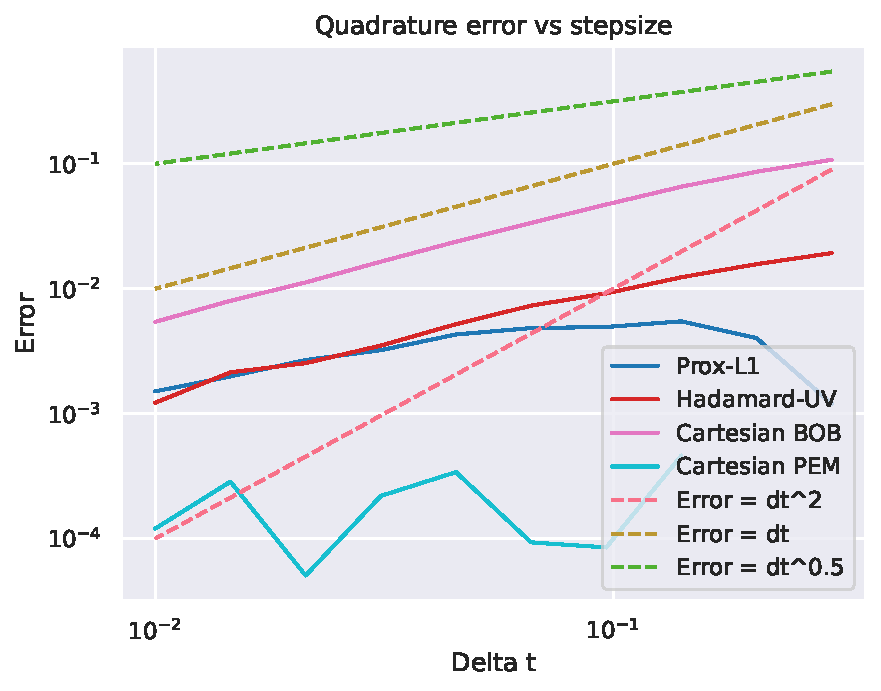
\includegraphics[width=1\linewidth]{IMG/loglog_plot_quad.pdf}
    \caption{Error of the stationary distribution for different stepsizes}
    \label{fig:error_1d}
\end{figure}
We carry out the experiment with $\phi(x) = x^2$. Figure \ref{fig:error_1d} shows the error between the mean of  $\phi(u\odot v)$  evaluated via these samples compared with the integral of the true density $\rho$ (i.e., \eqref{target}) against $\phi$ (we compute this numerically  using scipy.integrate). This procedure is also repeated for Proximal Langevin, as well as the cartesian discretizations, BOB and PEM. In general, we observe $\Oo(\deltat)$ for Proximal Langevin, Hadamard and BOB. PEM performed significantly better, although due to the Monte-Carlo error, it is difficult to say whether the quadrature error scaled as $\Oo(\deltat)$.


\subsection{20-dimensional regression}
We consider the case of $d=20$, and $A\in\RR^{40\times 20}$ is a random Gaussian matrix of mean zero and variance $\frac{1}{16m}$. We let $\lambda = \frac12 \norm{A^\top y}_\infty$ and $y=A x_0$ where $x_0$ is a 2-sparse vector.  For Proximal and Hadamard Langevin, BOB and PEM, we run $10^4$ burn-in iterations before recording $10^5$  samples,  while for Gibbs (due to its slower running time and faster convergence), we record $10^4$ samples after 10 burn-in samples. To assess the convergence of each scheme, we evaluate the effective sample size (ESS) which we computed using the package arviz \cite{arviz_2019}.   The sample means for each of the 20 dimensions are shown in Figure \ref{fig:means-dim20}. Figure \ref{fig:means-dim20} also shows the ESS in each dimension. Note that Gibbs has the highest ESS, followed by Hadamard. In general, for these low-dimensional settings, the  Gibbs sampler displays fast mean convergence behavior, and the Hadamard sampler also displays a similar pattern (although less sharp than the Gibbs sampler).

\begin{figure}[htbp]
    \centering
    % Row 1
    \begin{subfigure}{0.45\textwidth}
        \centering
        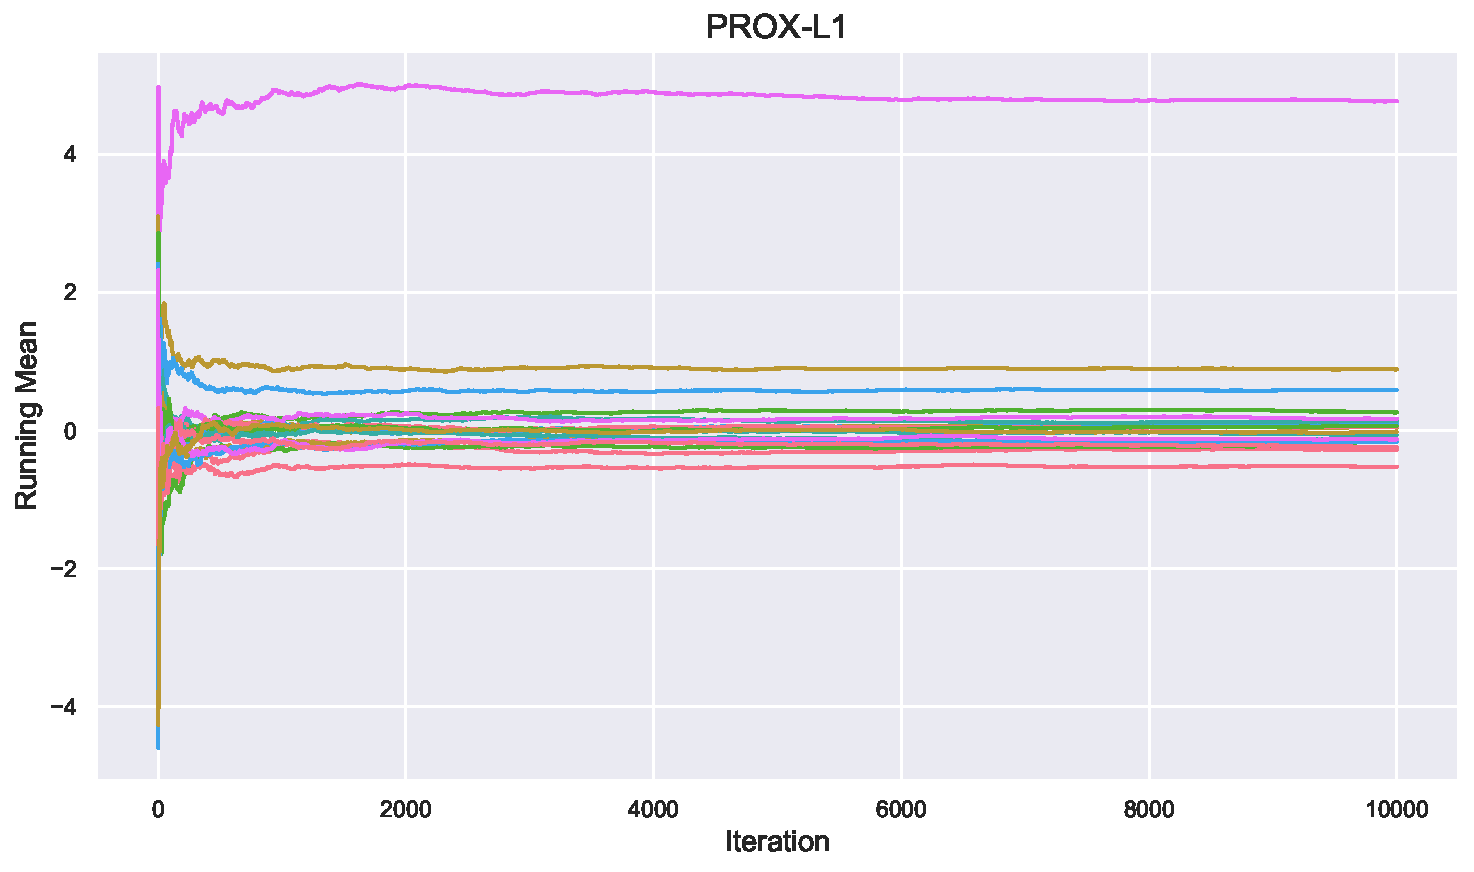
\includegraphics[width=\linewidth]{IMG/20d/mean_iter_eula.pdf}
        \caption{}
    \end{subfigure}
    \hfill
    \begin{subfigure}{0.45\textwidth}
        \centering
        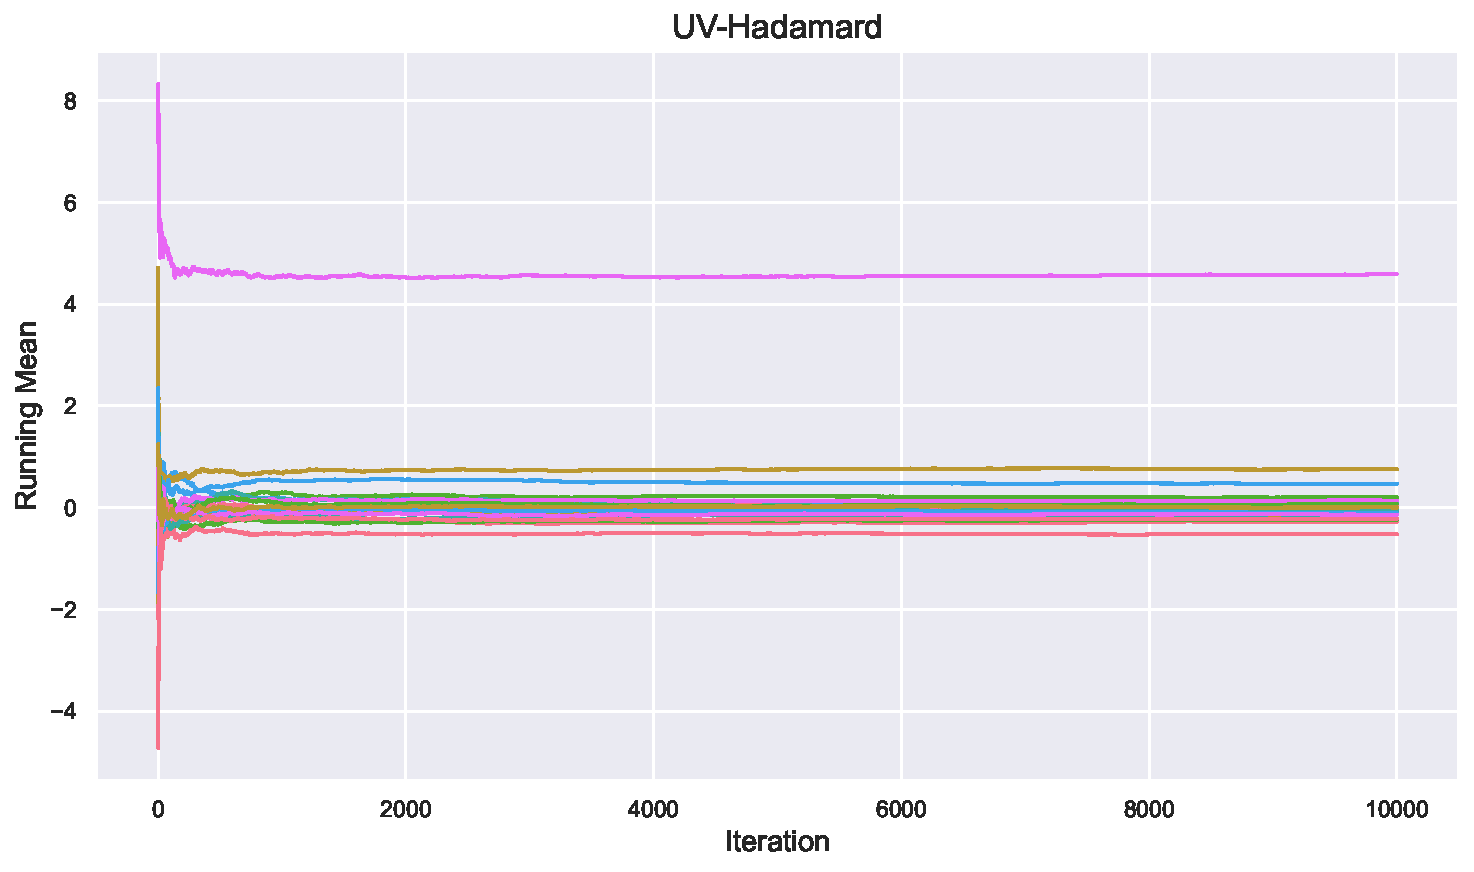
\includegraphics[width=\linewidth]{IMG/20d/mean_iter_uv.pdf}
        \caption{}
    \end{subfigure}

    \vspace{0.5cm}

    % Row 2
    \begin{subfigure}{0.45\textwidth}
        \centering
        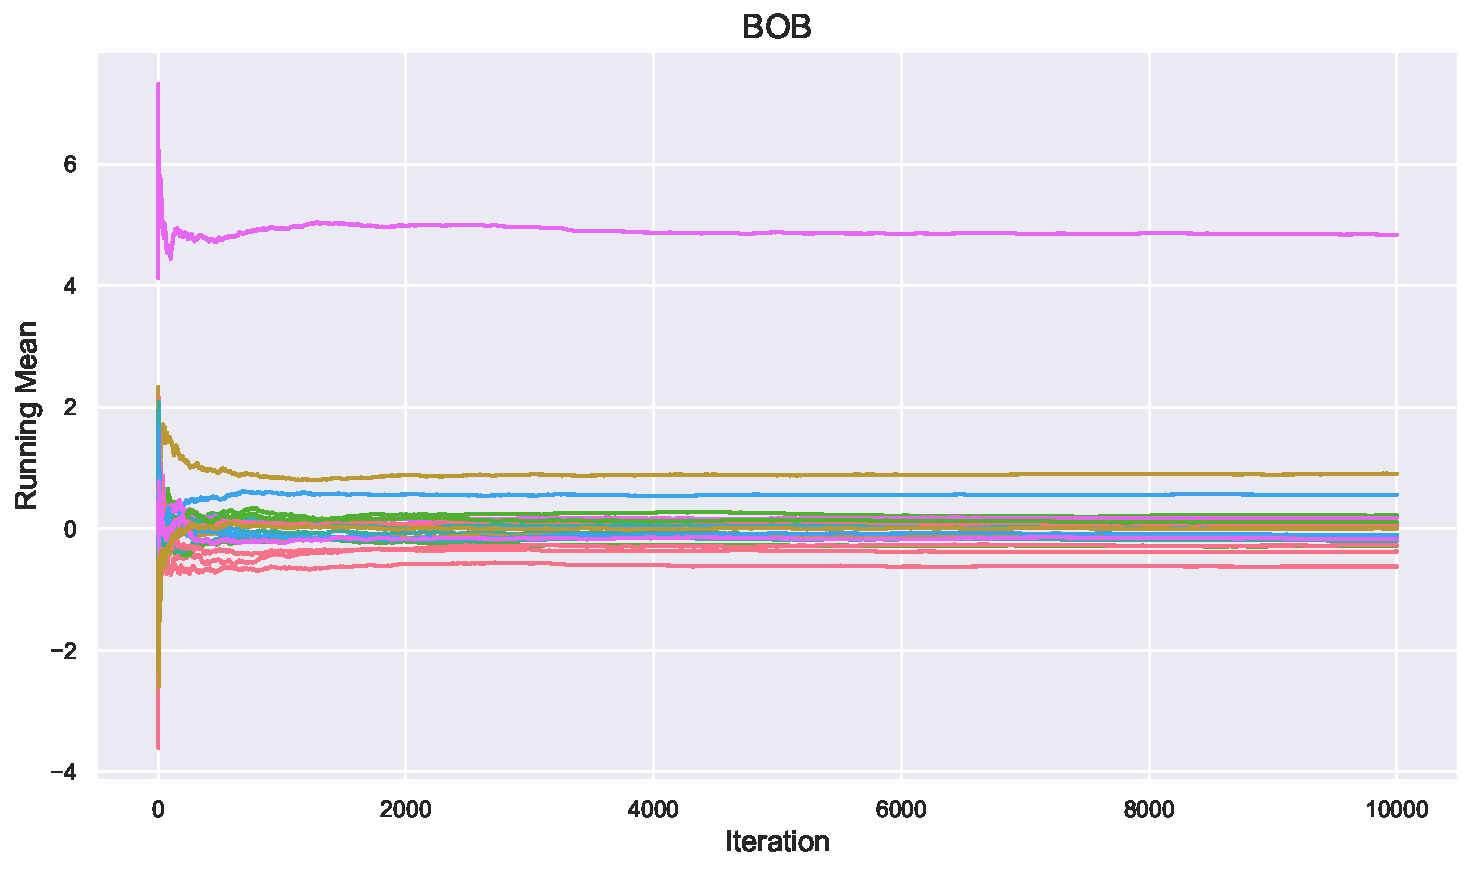
\includegraphics[width=\linewidth]{IMG/20d/mean_iter_bob.pdf}
        \caption{}
    \end{subfigure}
    \hfill
    \begin{subfigure}{0.45\textwidth}
        \centering
        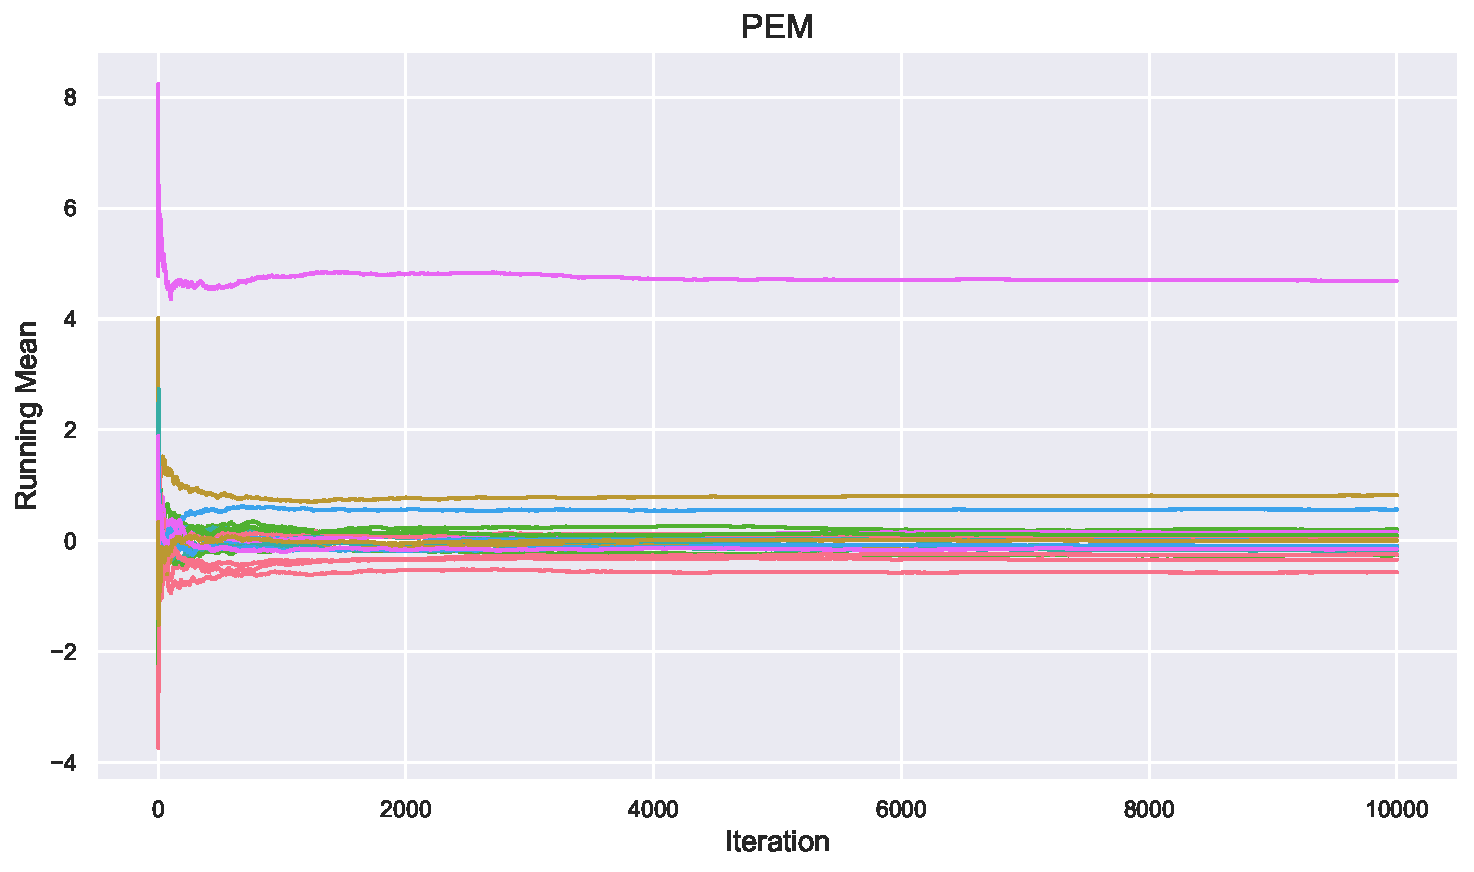
\includegraphics[width=\linewidth]{IMG/20d/mean_iter_pem.pdf}
        \caption{}
    \end{subfigure}

    \vspace{0.5cm}

    % Row 3
    \begin{subfigure}{0.45\textwidth}
        \centering
        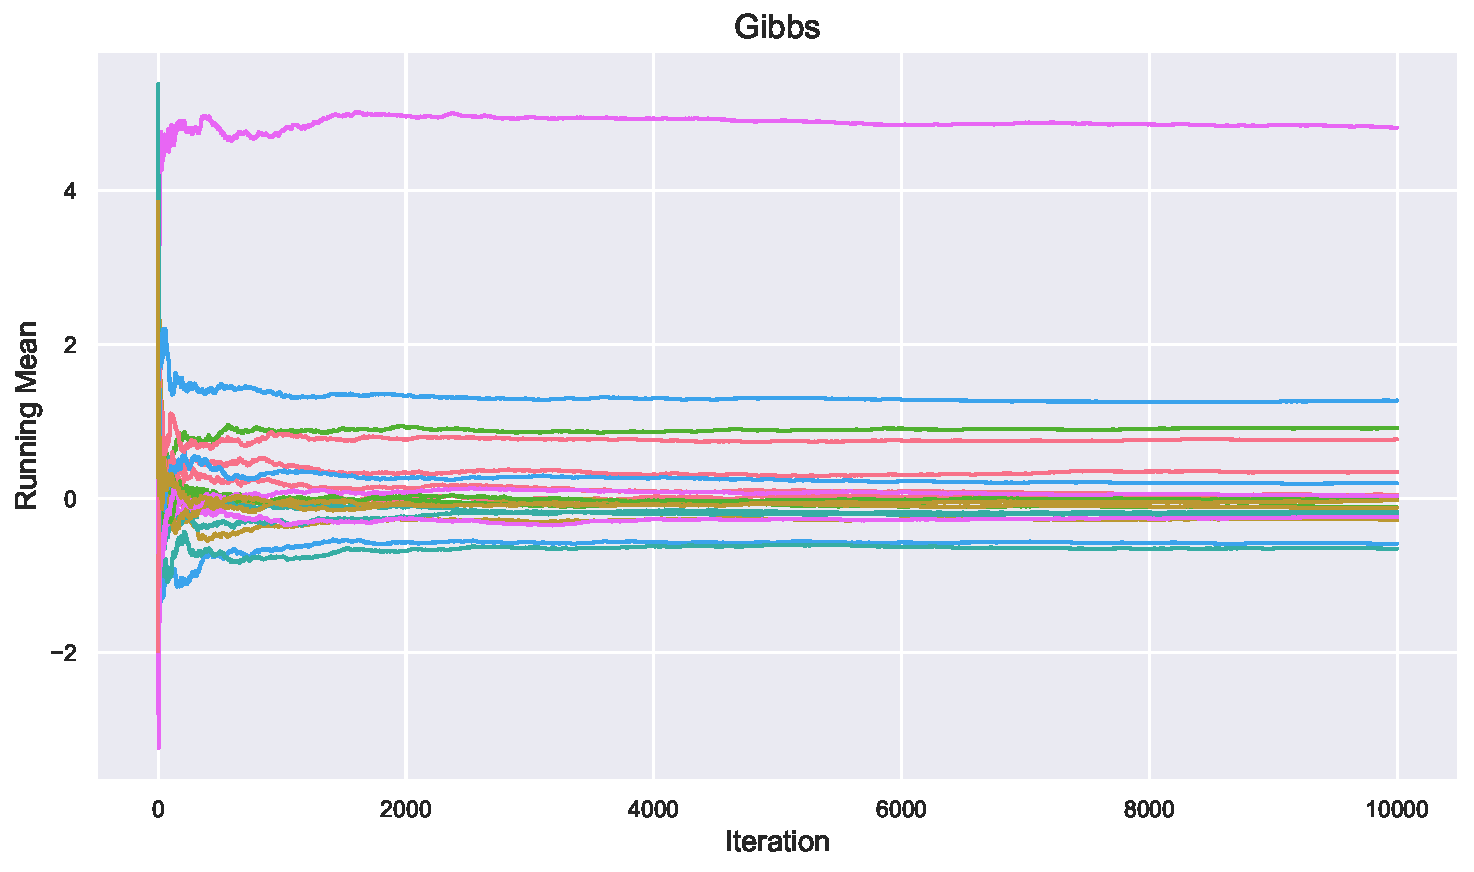
\includegraphics[width=\linewidth]{IMG/20d/mean_iter_gibbs.pdf}
        \caption{}
    \end{subfigure}
    \hfill
    \begin{subfigure}{0.45\textwidth}
        \centering
        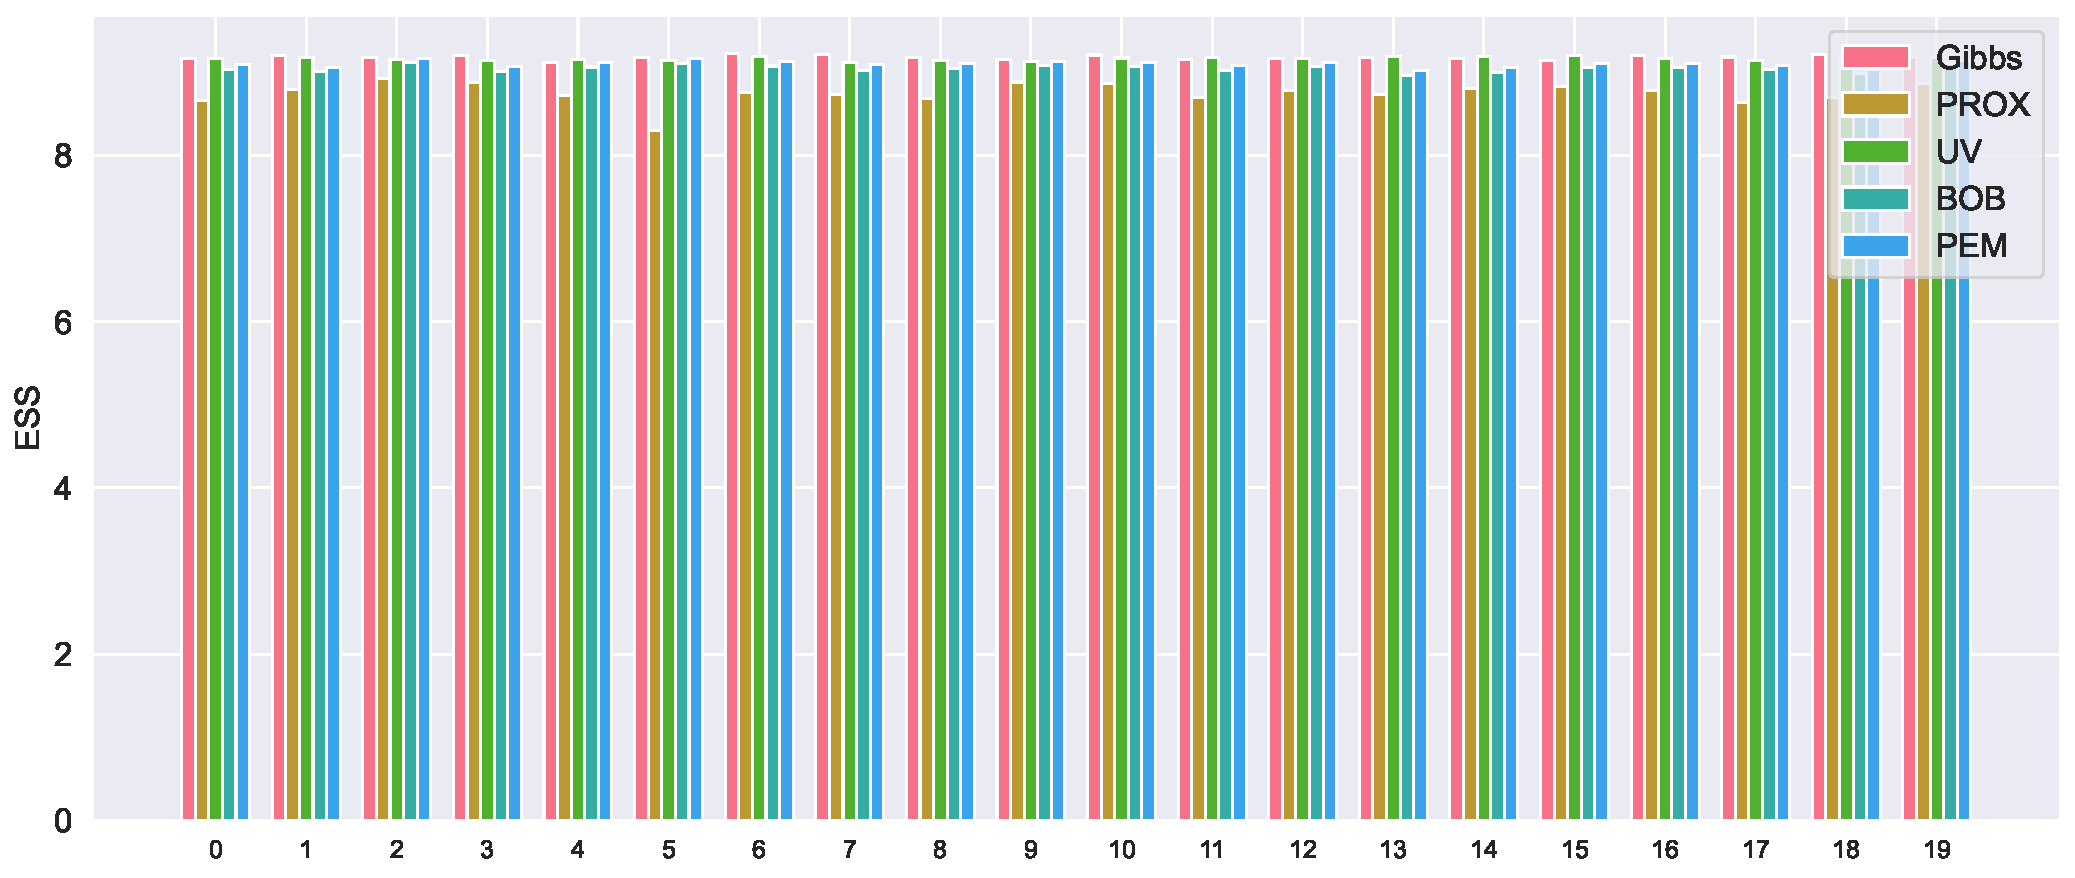
\includegraphics[width=\linewidth]{IMG/20d/ESS_samples.pdf}
        \caption{}
    \end{subfigure}

    \caption{(a)-(e) Running averages of iterates for various sampling methods; (f) Comparison of ESS of covariates for sampling methods.}
    \label{fig:means-dim20}
\end{figure}


%\begin{mdframed}[hidealllines=true,backgroundcolor=yellow!20]
%    If have time, add binary classifier experiment, demonstrating better mean performance.
%\end{mdframed}
    \subsection{Binary Classifier with Synthetic Dataset}
    \begin{comment}
        \begin{figure}
    \centering
    
\includegraphics[width=0.5\linewidth]{3d_boundary.pdf}
    \caption{Synthetic Dataset: Useful dimensions and decision boundary}
    \label{fig:db3d}
\end{figure}
    \end{comment}


\begin{figure}[htbp]
    \centering
    % Row 1
    \begin{subfigure}{0.45\textwidth}
        \centering
        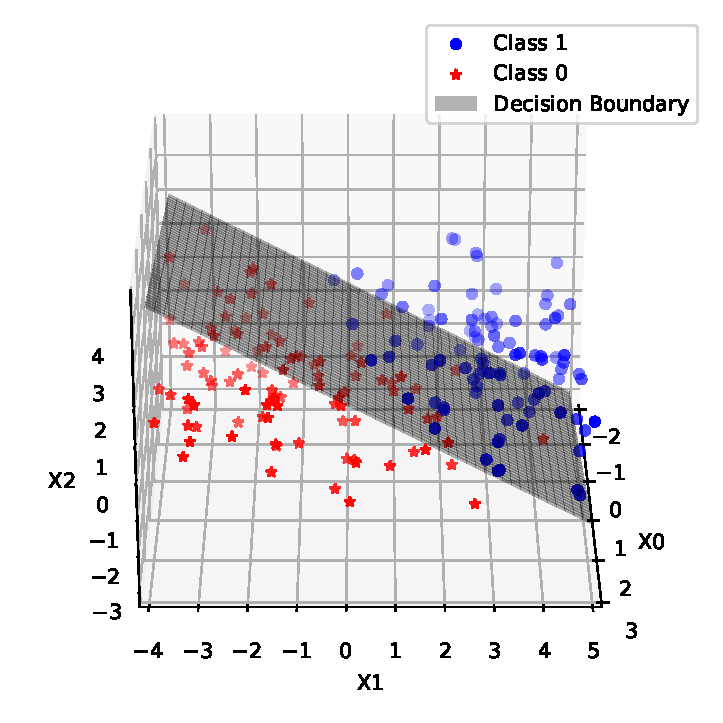
\includegraphics[width=\linewidth]{IMG/3d_boundary.pdf}
        \caption{}
    \end{subfigure}
    \hfill
    \begin{subfigure}{0.45\textwidth}
        \centering
        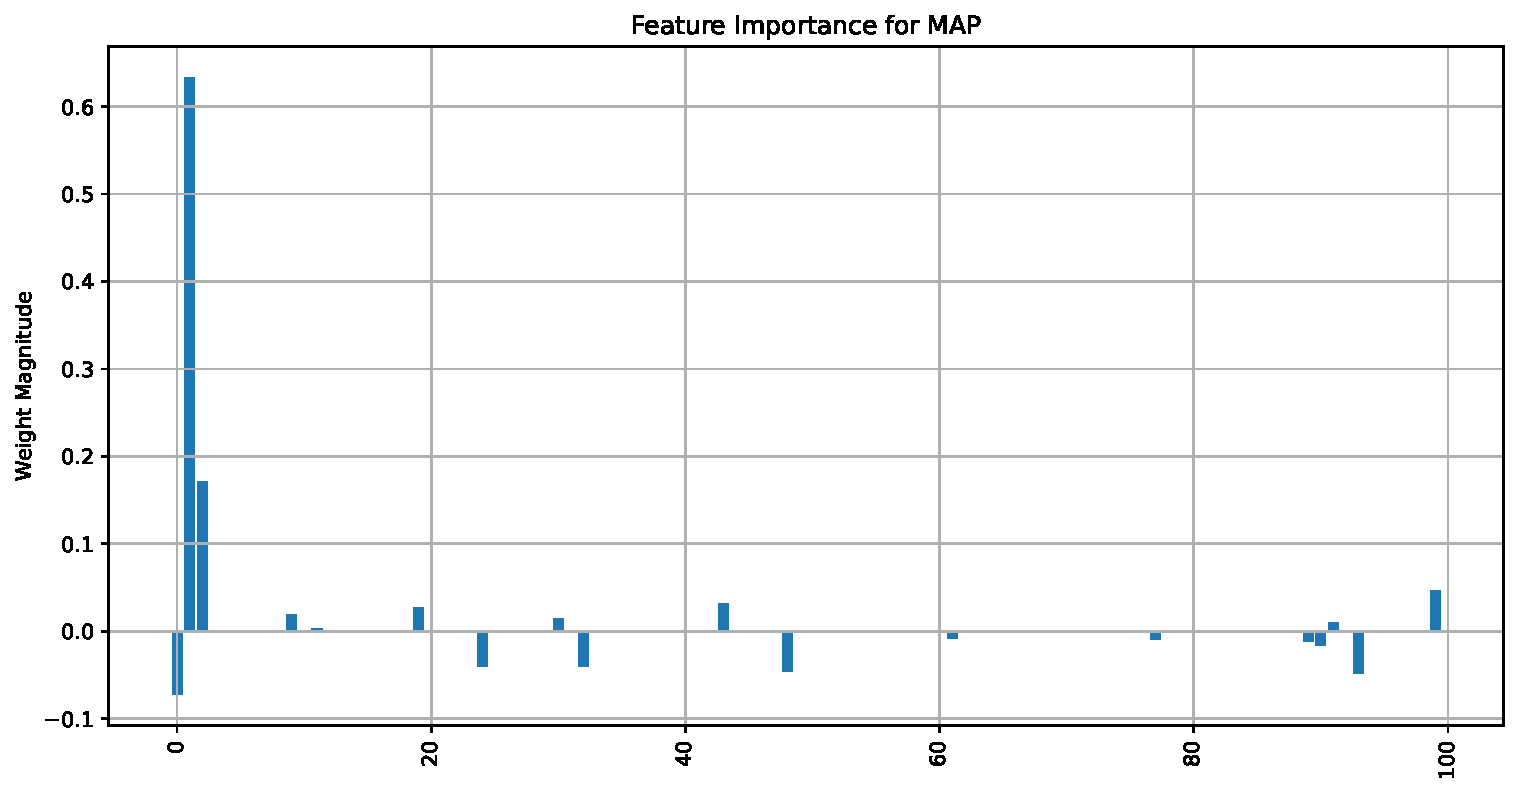
\includegraphics[width=\linewidth]{IMG/barplot_MAP.pdf}
        \caption{}
    \end{subfigure}

    \caption{(left) Example synthetic Dataset: Useful dimensions and decision boundary; (right) Typical MAP for higher value of lambda (note the non-zero useful dimensions).}
    \label{fig:db3d}
\end{figure}


\begin{comment}
    We generate a synthetic dataset in the following way. The domain is $\mathbb{R}^{k_U + k_N}$, where $k_U$ is the number of `useful' dimensions and $k_N$ is the number of noisy dimensions. We generate $n$ samples of type $(X_0,X_1,\hdots,X_{k_U-1},Y_0,Y_1,\hdots,Y_{k_N-1})$, such that in the useful dimensions $(X_0,X_1,\cdots,X_{k_U-1})$, these samples are linearly separable (see Figure below \ref{fig:db3d}), while the noisy dimensions $(Y_0,Y_1,\hdots,Y_{k_N-1})$ are distributed as $\mathcal{N}(\mu_N,\sigma_N)$. The idea is that a linear classifier with no regularization will train non-zero weights associated with the noisy dimensions $Y_i$, thus reducing classification accuracy, while a sparsity-inducing regularizer will put more emphasis on the useful dimensions $X_i$. In our setup, we will use $k_U = 3, k_N = 97, \mu_N = 0,\sigma_N = 1$, with a linear decision boundary, shown in Figure \ref{fig:db3d}, where the data entries are split between the two classes approximately evenly. We run the following experiment: Using $G(x)=\sum_{i=1}^m \log( 1+ \exp(-y_i A_i^\top x) )$, i.e. the logistic cost function, where $A \in \mathbb{R}^{200 \times 100},y \in \mathbb{R}^{200}$ are 200 training entries of the synthetic dataset and corresponding labels, we train the proximal and uv Langevin, BOB and PEM samplers, running the chains until burn-in, after which we collect 10,000 samples. For these, we compute the mean predictive accuracy and corresponding mean ROC/AUC score over the test set, generated in a similar fashion to that of the training set above, but with 50 entries. For robustness, we replicate this experiment 100 times, regenerating the training and test sets every time and ultimately recording the median of the mean predictive accuracies and mean ROC/AUC scores
\end{comment}
We construct a synthetic binary classification dataset as follows. The data domain is 
\[
\mathbb{R}^{k_U + k_N},
\]
where $k_U$ denotes the number of informative dimensions, and $k_N$ denotes the number of noisy dimensions. Each data point is of the form  
\[
(X_0, X_1, \dots, X_{k_U-1}, Y_0, Y_1, \dots, Y_{k_N-1}),
\]  
where the subvector $(X_0, X_1, \dots, X_{k_U-1})$ lies in a region that is linearly separable between the two classes (see Figure~\ref{fig:db3d}), and the subvector $(Y_0, Y_1, \dots, Y_{k_N-1})$ consists either of i.i.d. noise drawn from the Gaussian distribution $Y_i \sim \mathcal{N}(\mu_N, \sigma_N^2)$ or jointly distributed noise drawn from the multivariate Gaussian distribution
\[
(Y_0, Y_1, \dots, Y_{k_N-1}) \sim \mathcal{N}(\mu_N \mathbf{1}, \Sigma_N),
\]
where $\Sigma_N \in \mathbb{R}^{k_N \times k_N}$ is a covariance matrix with unit variances on the diagonal and off-diagonal entries equal to $\rho_N \sigma_N^2$,  introducing pairwise correlation between the noise components. To be more precise, the effect of $\rho_N$ scales linearly via
\[
\Sigma_N = \sigma_N^2 \left( \rho_N \mathbf{1} \mathbf{1}^\top + (1 - \rho_N) I \right).
\] 
The above construction is intended to illustrate the effects of regularization: a linear classifier trained without any regularization is likely to assign nonzero weights to the noisy dimensions $Y_i$, thereby reducing classification accuracy. In contrast, a sparsity-inducing regularizer (or prior) should encourage the model to focus on the useful features $X_i$ and suppress contributions from noise. For our setup, we choose
\[
k_U = 3, \quad k_N \in \{27, 97\}, \quad \mu_N = 0, \quad \sigma_N = 1, \quad \rho_N \in \{0, 0.5\}
\]
yielding four experiments, where we have a) either a 30- or 100-dimensional feature space and b) either i.i.d. noise or correlated noise. The decision boundary separating the two classes is linear and chosen to produce approximately balanced class labels (see Figure~\ref{fig:db3d}). To evaluate the performance of different Bayesian sampling methods, we minimize the logistic loss
\begin{equation} \label{eq:binary_logistic}
    G(x) = \sum_{i=1}^m \log\left(1 + \exp(-y_i A_i^\top x)\right),
\end{equation}
where $A \in \mathbb{R}^{200 \times 100}$ is the design matrix containing 200 training samples and $y \in \{-1, 1\}^{200}$ are the associated class labels. We compare the performance of four sampling-based inference algorithms: Proximal Langevin, UV-Langevin, BOB, and PEM. Each sampler is run until convergence (after discarding an initial burn-in phase), after which we collect 10,000 posterior samples. Using these samples, we compute the mean predictive classification accuracy and the mean ROC/AUC score on a test set of 50 points generated in the same fashion as the training set. For robustness, the entire experiment is repeated 100 times, with both the training and test datasets regenerated for each run. We report the median of the mean predictive accuracies and AUC scores across these 100 repetitions and compare them to a deterministic Lasso solver. The results for all experiments are visualized in Tables \ref{tab:train_test_accuracy_binary}-\ref{tab:train_test_accuracy_binary_small_corr}. This setup was inspired by that of Mallick and Yi \cite{mallick2014Bayesian}, however in our case, the optimal hyperparameter $\lambda$ was chosen via gridsearch for both the deterministic solver and Bayesian samplers. We expected median mean test accuracy to be higher for the Bayesian samplers, as opposed to the Lasso solver, similar to the findings of Mallick and Yi. However, this was not the case and Lasso outperformed the other methods in all four experiments.
\begin{table}[h!]
    \centering
    \begin{tabular}{l c c}
        \hline
        \textbf{Classifier} & \textbf{Median Mean Accuracy} & \textbf{Median Mean ROC/AUC} \\
        \hline
        Lasso & 84\%  & 0.9127  \\
        UV-Hadamard & 83.7\%  & 0.9165  \\
        Prox-L1       & 83.77\%  & 0.9183  \\
        BOB                 & 83.55\%  & 0.9175  \\
        PEM      & 82.8\%  & 0.9157  \\
        \hline
    \end{tabular}
    \caption{Synthetic Dataset with 97 i.i.d. noisy features: Median Mean Accuracy and Median Mean ROC/AUC score over 100 replications.}
    \label{tab:train_test_accuracy_binary}
\end{table}

\begin{table}[h!]
    \centering
    \begin{tabular}{l c c}
        \hline
        \textbf{Classifier} & \textbf{Median Mean Accuracy} & \textbf{Median Mean ROC/AUC} \\
        \hline
        Lasso & 86\%  & 0.9191  \\
        UV-Hadamard & 79.97\%  & 0.9107  \\
        Prox-L1       & 79.12\%  & 0.9111  \\
        BOB                 & 80.24\%  & 0.9091  \\
        PEM      & 80.22\%  & 0.9091  \\
        \hline
    \end{tabular}
    \caption{Synthetic Dataset with 97 correlated noisy features: Median Mean Accuracy and Median Mean ROC/AUC score over 100 replications.}
    \label{tab:train_test_accuracy_binary_corr}
\end{table}

\begin{table}[h!]
    \centering
    \begin{tabular}{l c c}
        \hline
        \textbf{Classifier} & \textbf{Median Mean Accuracy} & \textbf{Median Mean ROC/AUC} \\
        \hline
        Lasso & 86\%  & 0.9191  \\
        UV-Hadamard & 82.22\%  & 0.9201  \\
        Prox-L1       & 82.44\%  & 0.9149  \\
        BOB                 & 82.19\%  & 0.9194  \\
        PEM      & 79.76\%  & 0.9148  \\
        \hline
    \end{tabular}
    \caption{Synthetic Dataset with 27 uncorrelated noisy features: Median Mean Accuracy and Median Mean ROC/AUC score over 100 replications.}
    \label{tab:train_test_accuracy_binary_small_uncorr}
\end{table}

\begin{table}[h!]
    \centering
    \begin{tabular}{l c c}
        \hline
        \textbf{Classifier} & \textbf{Median Mean Accuracy} & \textbf{Median Mean ROC/AUC} \\
        \hline
        Lasso & 86\%  & 0.9227  \\
        UV-Hadamard & 82.23\%  & 0.9278  \\
        Prox-L1       & 81.96\%  & 0.9249  \\
        BOB                 & 81.95\%  & 0.9228  \\
        PEM      & 81.94\%  & 0.9228  \\
        \hline
    \end{tabular}
    \caption{Synthetic Dataset with 27 correlated noisy features: Median Mean Accuracy and Median Mean ROC/AUC score over 100 replications.}
    \label{tab:train_test_accuracy_binary_small_corr}
\end{table}

\subsection{Binary Classifier with Cancer Dataset}
We set up another binary classification problem, this time using the Wisconsin breast cancer dataset\footnote{https://www.kaggle.com/datasets/uciml/breast-cancer-wisconsin-data}, with 569 total samples, each containing 30 features. This dataset is divided into 357 benign and 212 malignant samples. We split this into training and test sets of size 455 and 114, respectively. We use the same logistic loss $G$ as in (\ref{eq:binary_logistic}). For Hadamard, proximal Langevin, as well as the BOB and PEM schemes, we simulate for $\beta = 5, 100$, using $10^5$ burn-in iterations and $3\times10^5$ sampling iterations, with a subsampling frequency of 1000, for a total of 3000 final uncorrelated samples. In Figures \ref{fig:cancer5} and \ref{fig:cancer100} you can see the mean weights and quantiles for the cases $\beta = 5$ and $\beta = 100$, respectively. In both cases, we observe the highest variance in mean non-zero weights. Interestingly, the mean test accuracy for the Bayesian methods was higher than for deterministic lasso (used to compute the MAP), when $\beta = 5$. Here, the test accuracy for the deterministic solution was 96.49\%, while the mean test accuracy (over 3000 samples) for all Bayesian methods was 97.37\%. On the other hand, for higher values of $\beta$, both the mean test accuracy for the Bayesian methods and the test accuracy for LASSO were very similar, which is expected as the samples in this case are all concentrated around the MAP. Additionally, at lower $\beta$, the samples had a lower mean sklearn logistic score. Both this and the higher mean test accuracy scores suggests that samples produced at lower $\beta$ could have useful generalizing properties.

\begin{figure}[htbp]
    \centering
    % Row 1
    \begin{subfigure}{1\textwidth}
        \centering
        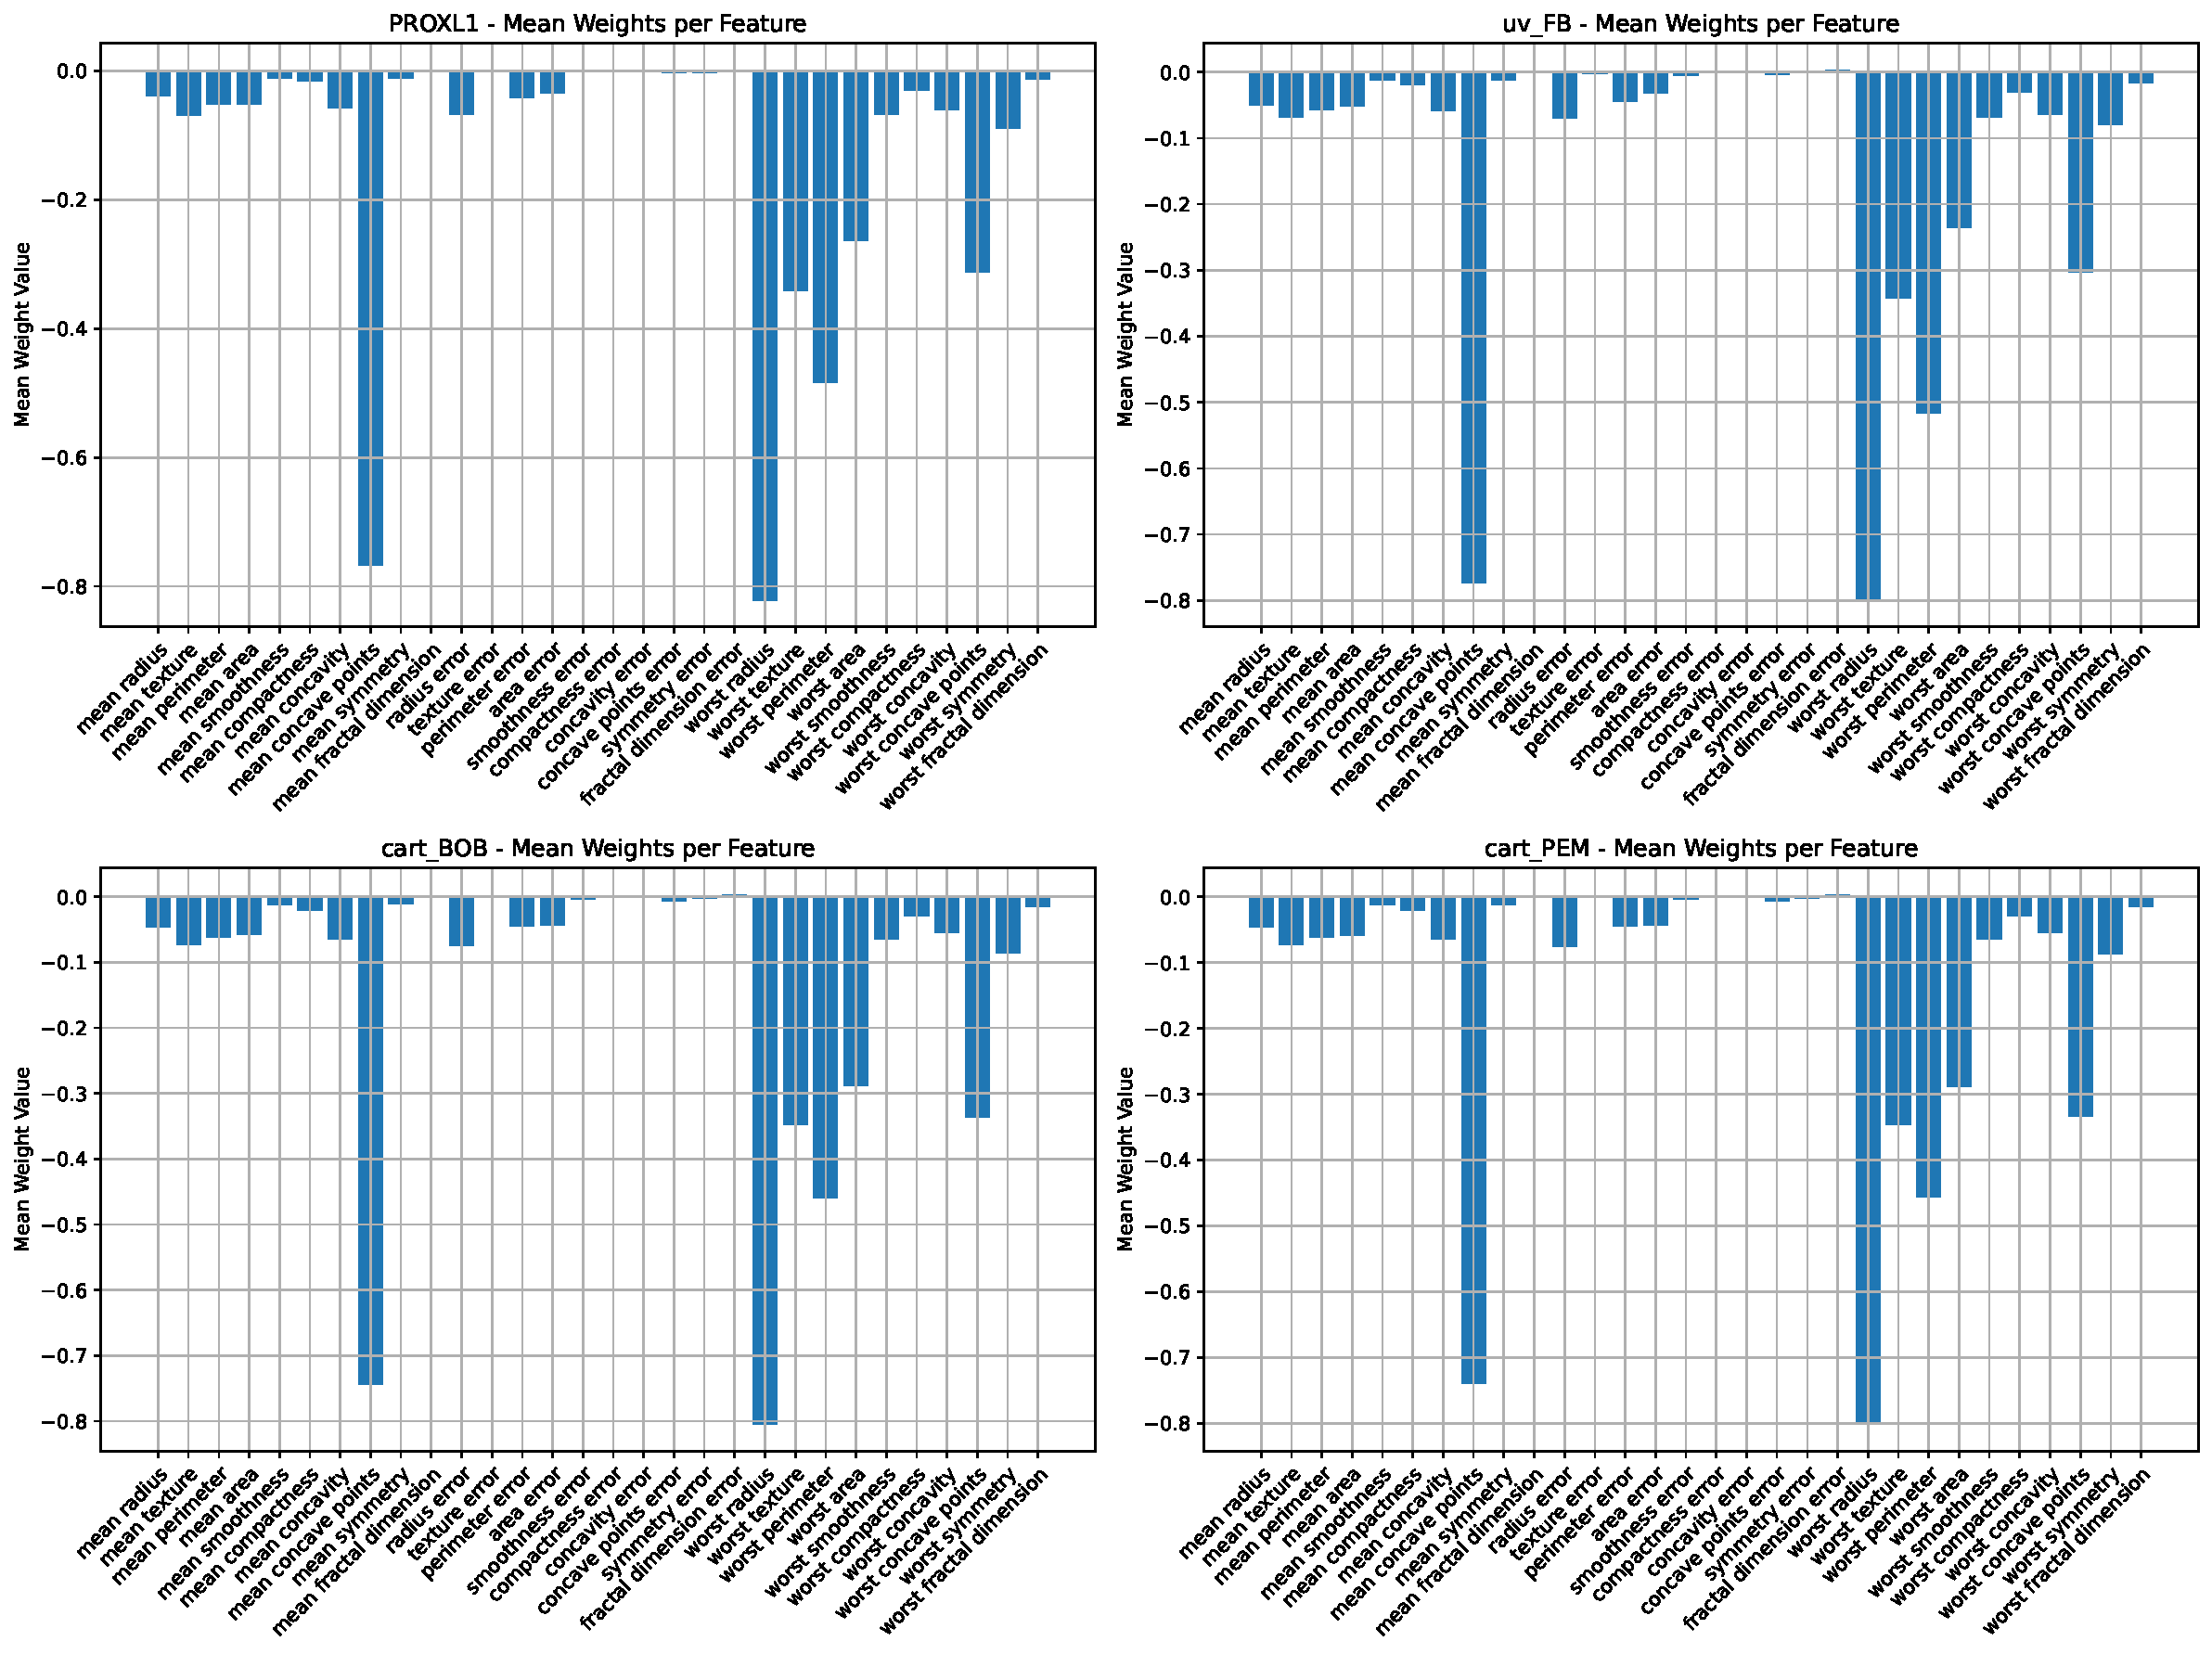
\includegraphics[width=\linewidth]{IMG/wisconsin/beta5/weight_means.pdf}
        \caption{Means}
    \end{subfigure}

    \vspace{0.5cm}

    % Row 2
    \begin{subfigure}{1\textwidth}
        \centering
        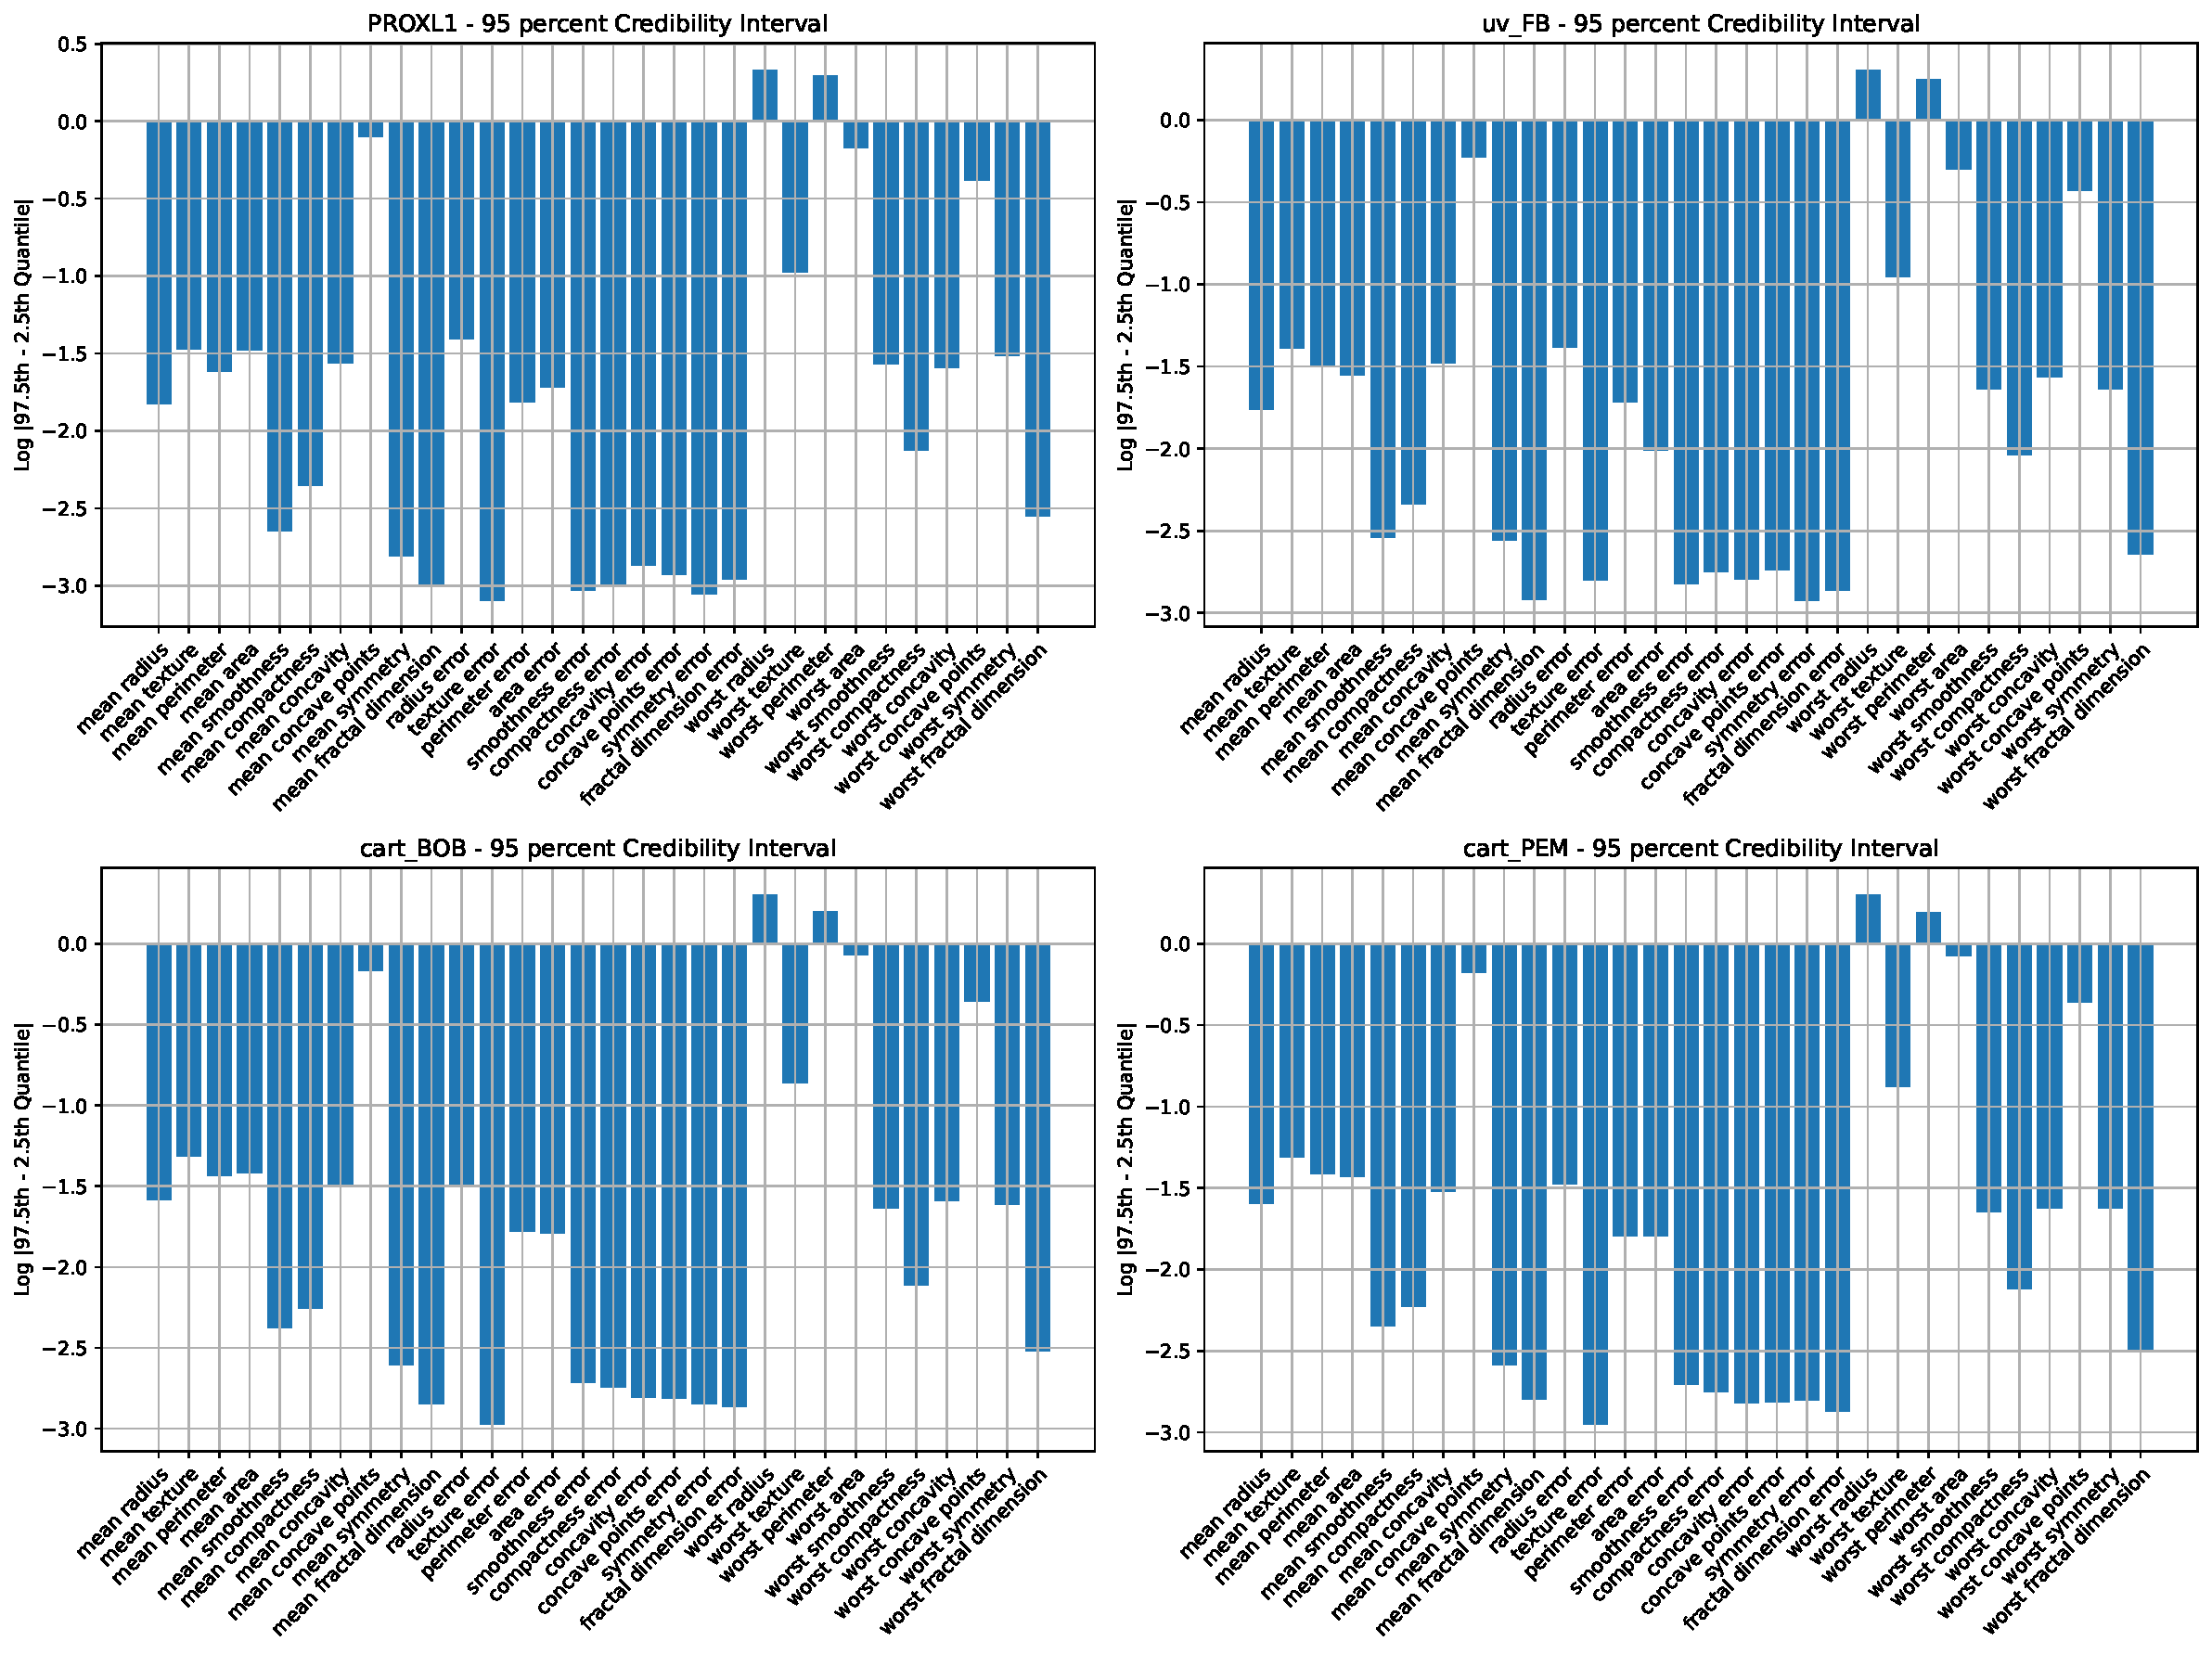
\includegraphics[width=\linewidth]{IMG/wisconsin/beta5/weight_quantile.pdf}
        \caption{95\% Log-Quantiles}
    \end{subfigure}
    

    \caption{Wisconsin cancer test data: mean weights and quantiles for $\beta = 5$}
    \label{fig:cancer5}
\end{figure}


\begin{figure}[htbp]
    \centering
    % Row 1
    \begin{subfigure}{1\textwidth}
        \centering
        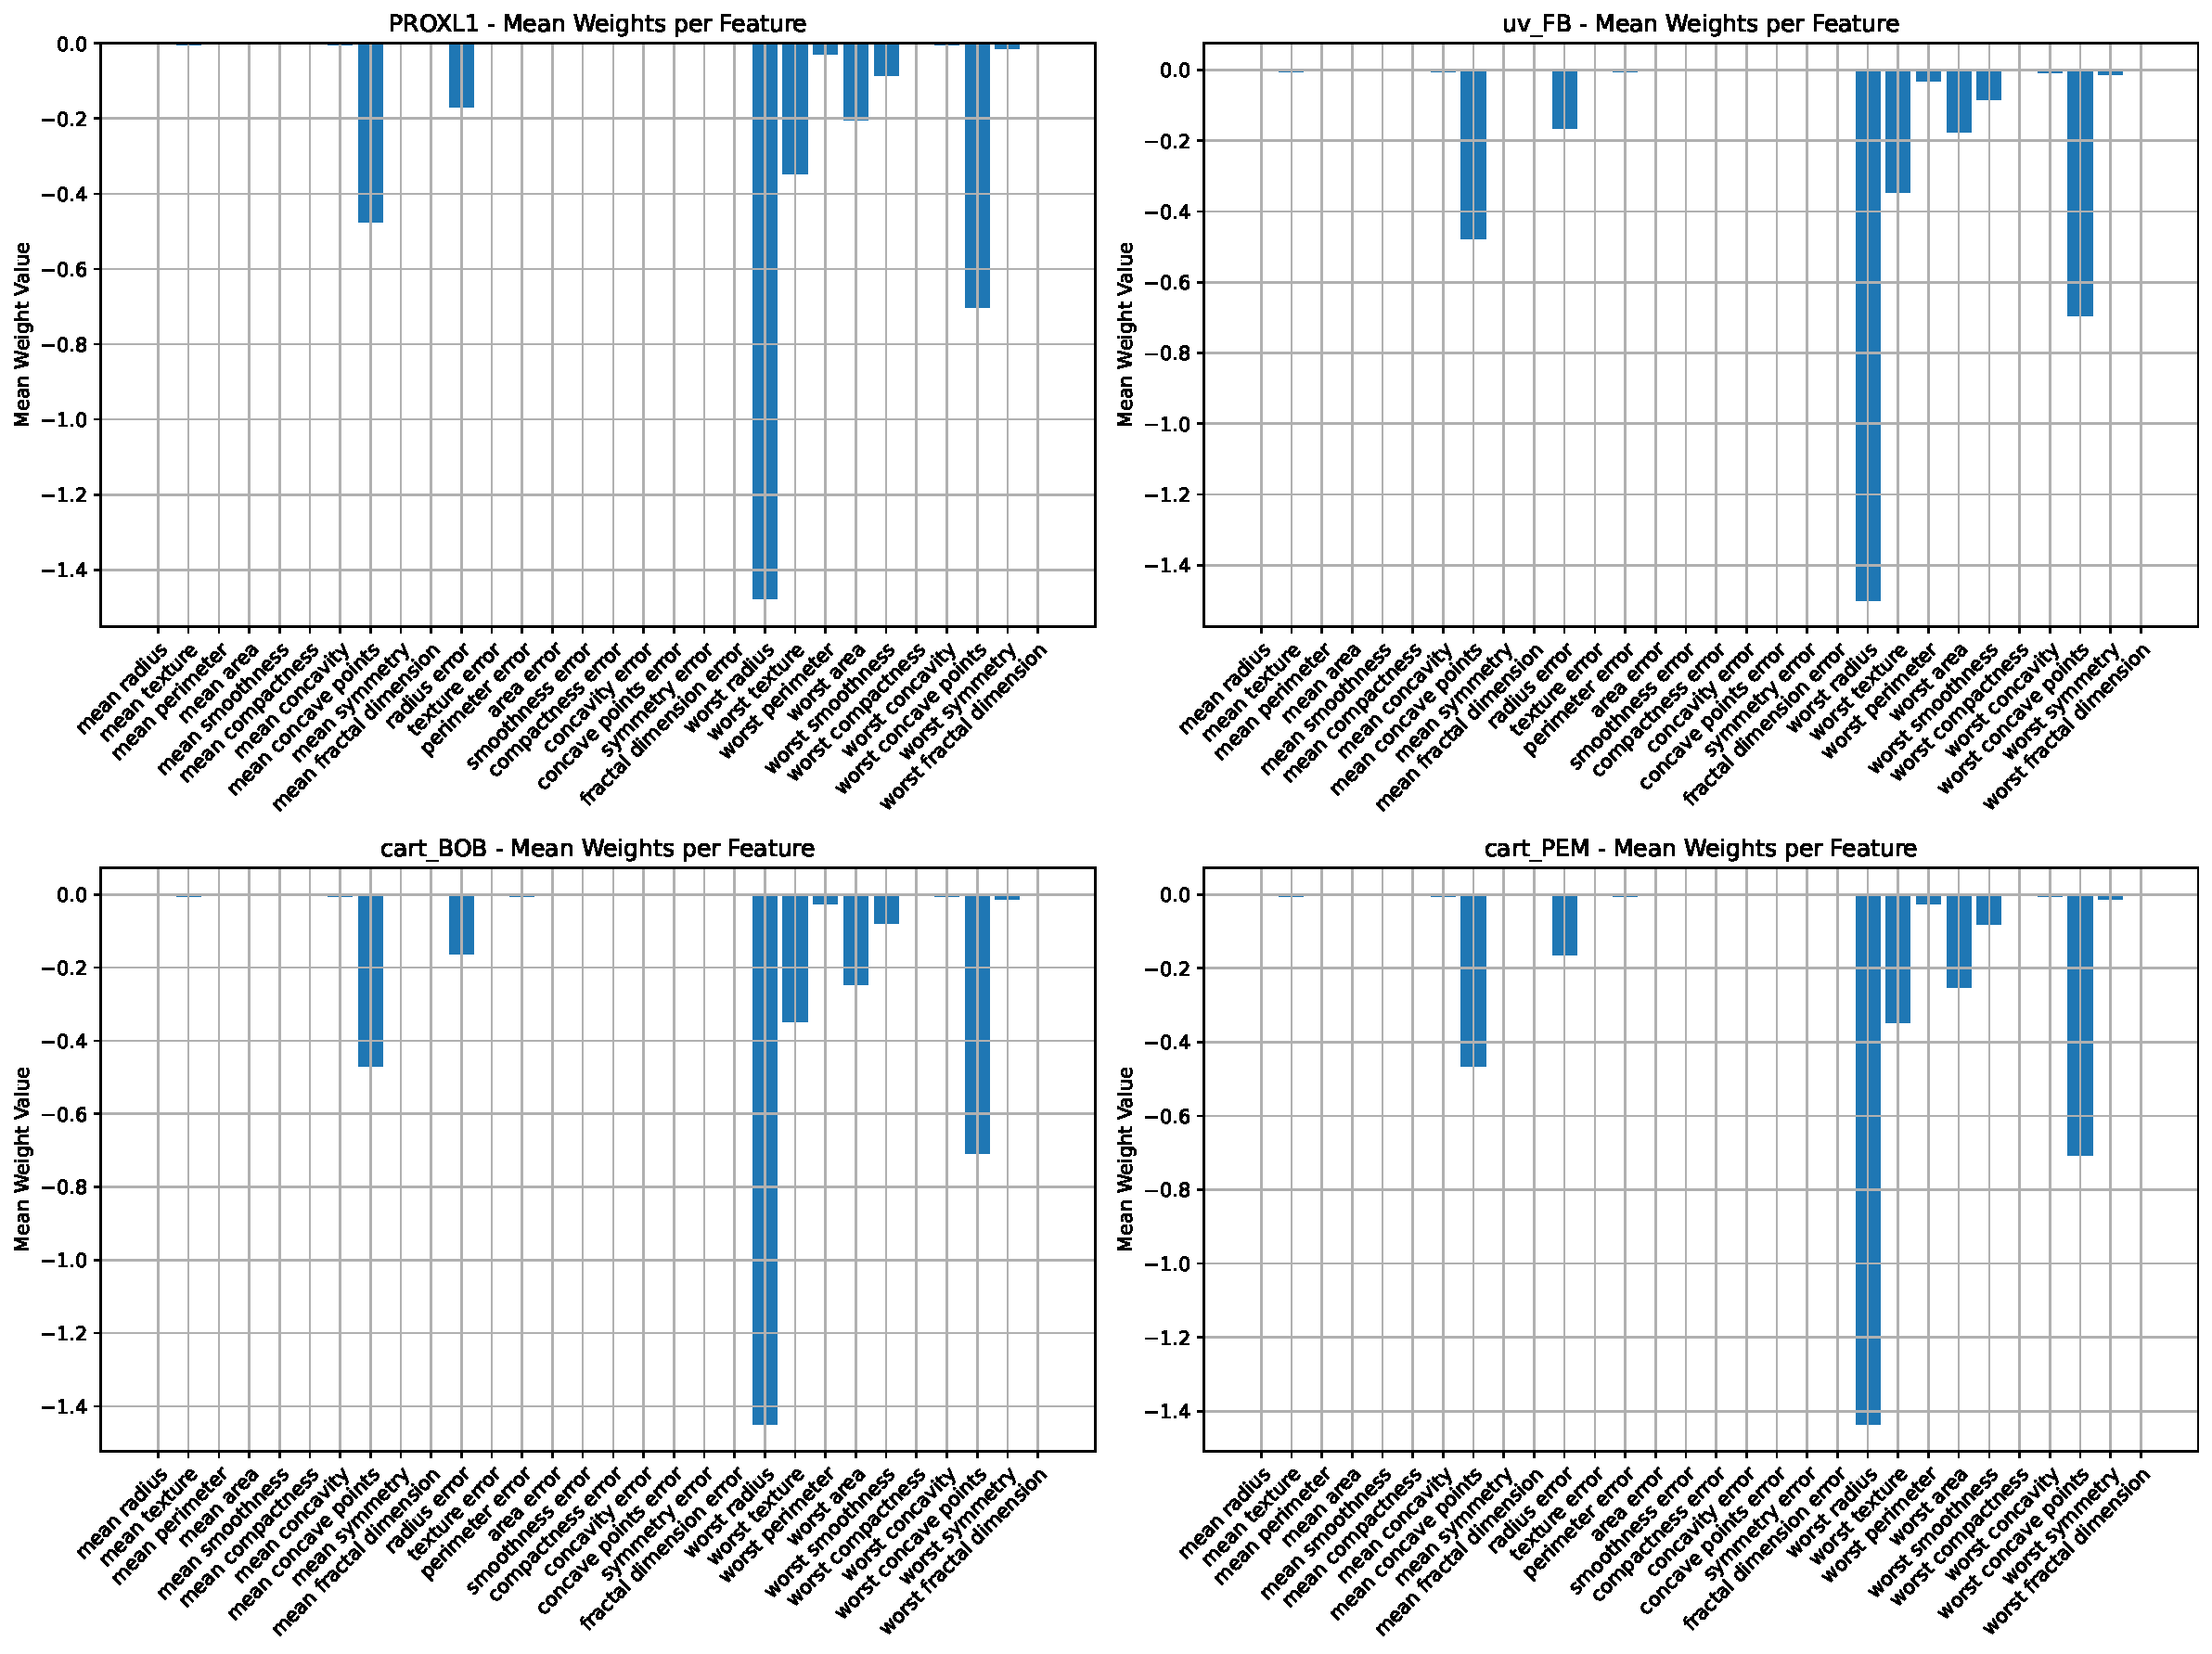
\includegraphics[width=\linewidth]{IMG/wisconsin/beta100/weight_means.pdf}
        \caption{Means}
    \end{subfigure}

    \vspace{0.5cm}

    % Row 2
    \begin{subfigure}{1\textwidth}
        \centering
        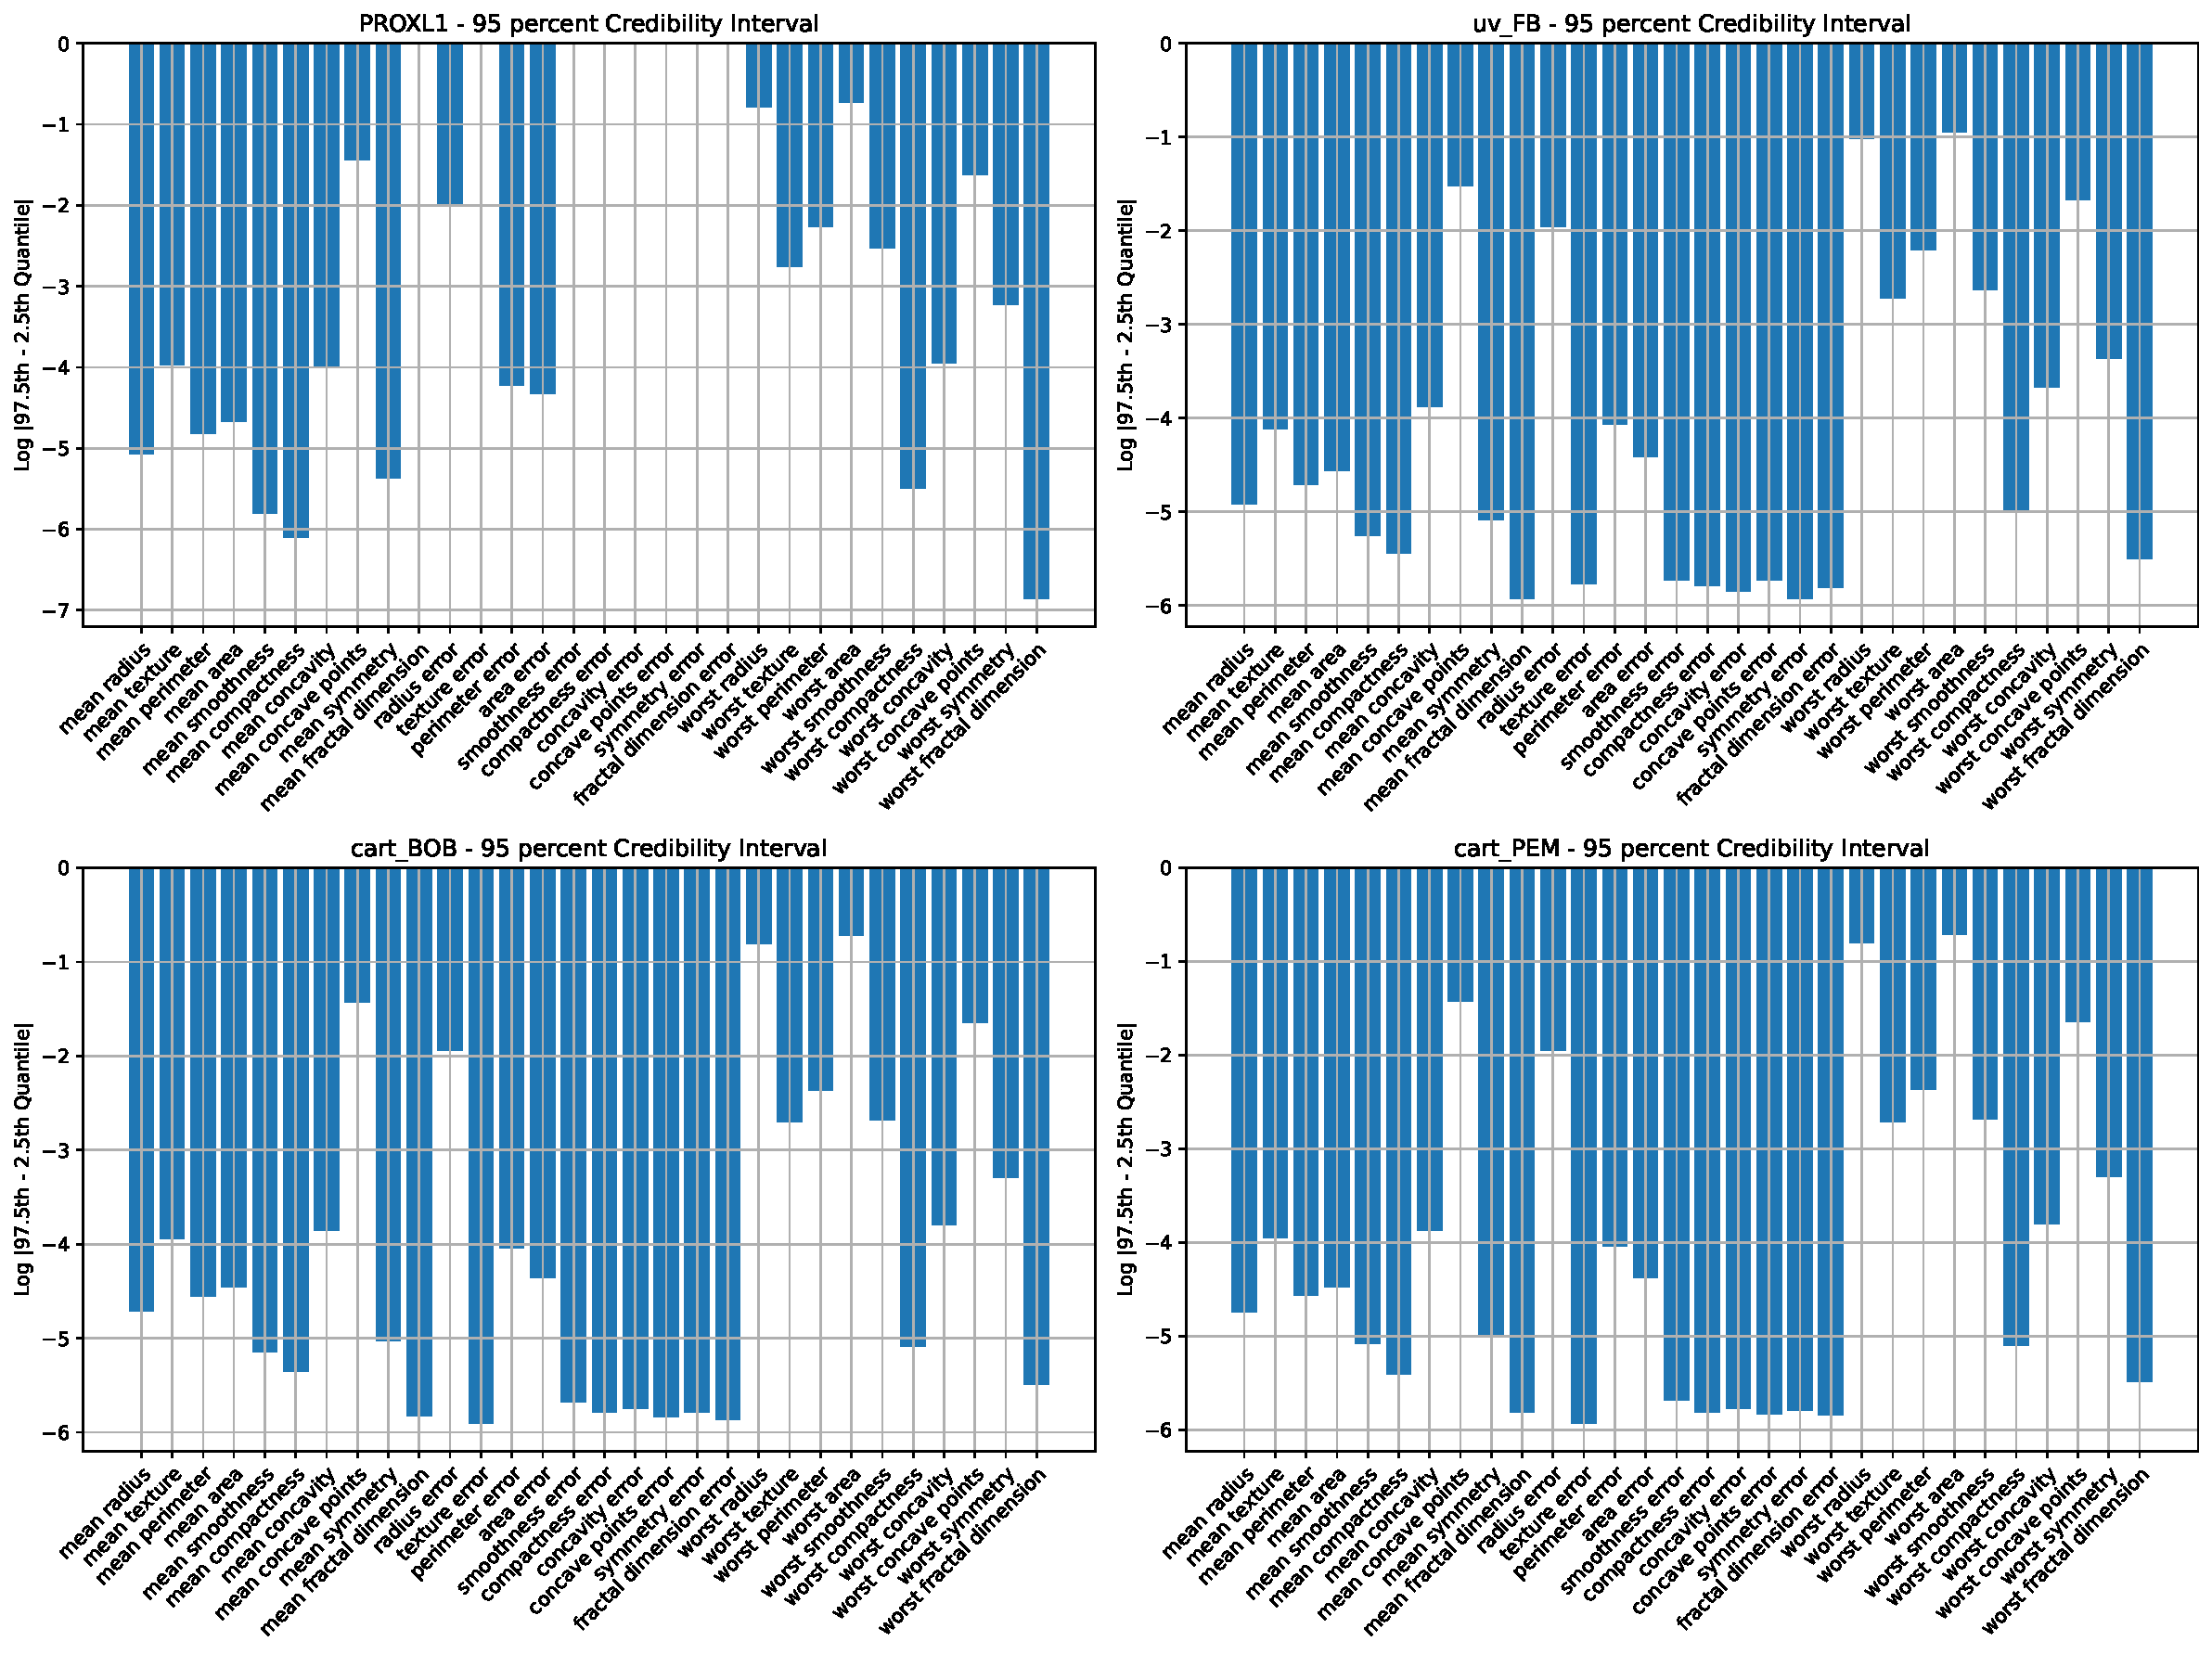
\includegraphics[width=\linewidth]{IMG/wisconsin/beta100/weight_quantile.pdf}
        \caption{95\% Log-Quantiles}
    \end{subfigure}
    

    \caption{Wisconsin cancer test data: mean weights and quantiles for $\beta = 100$}
    \label{fig:cancer100}
\end{figure}

\subsection{1D Deconvolution with Haar wavelets}
We consider Gaussian deconvolution of a piecewise-constant signal (length $d = 1024$). The operator $A$ here represents a convolution with an orthogonal haar transform. We set $\lambda = 1$. We run Proximal and Hadamard Langevin, as well as the BOB and PEM samplers, each with stepsize $\tau = 0.01$, for 5000 burn-in iterations, recording 10,000 out of $10^5$ samples (subsampling every 10th). In Figure \ref{fig:haar_1d} we present the sample means, credibility intervals and autocorrelation values at maximum lag of 50. Note that the correlation for the proximal Langevin samples decays slower in comparison to other methods. Additionally, for all methods exhibit larger credibility intervals around the jumps, which is expected as the reconstruction of the precise jump locations is more unstable.
\begin{figure}[htbp]
    \centering
    % Row 1
    \begin{subfigure}{0.45\textwidth}
        \centering
        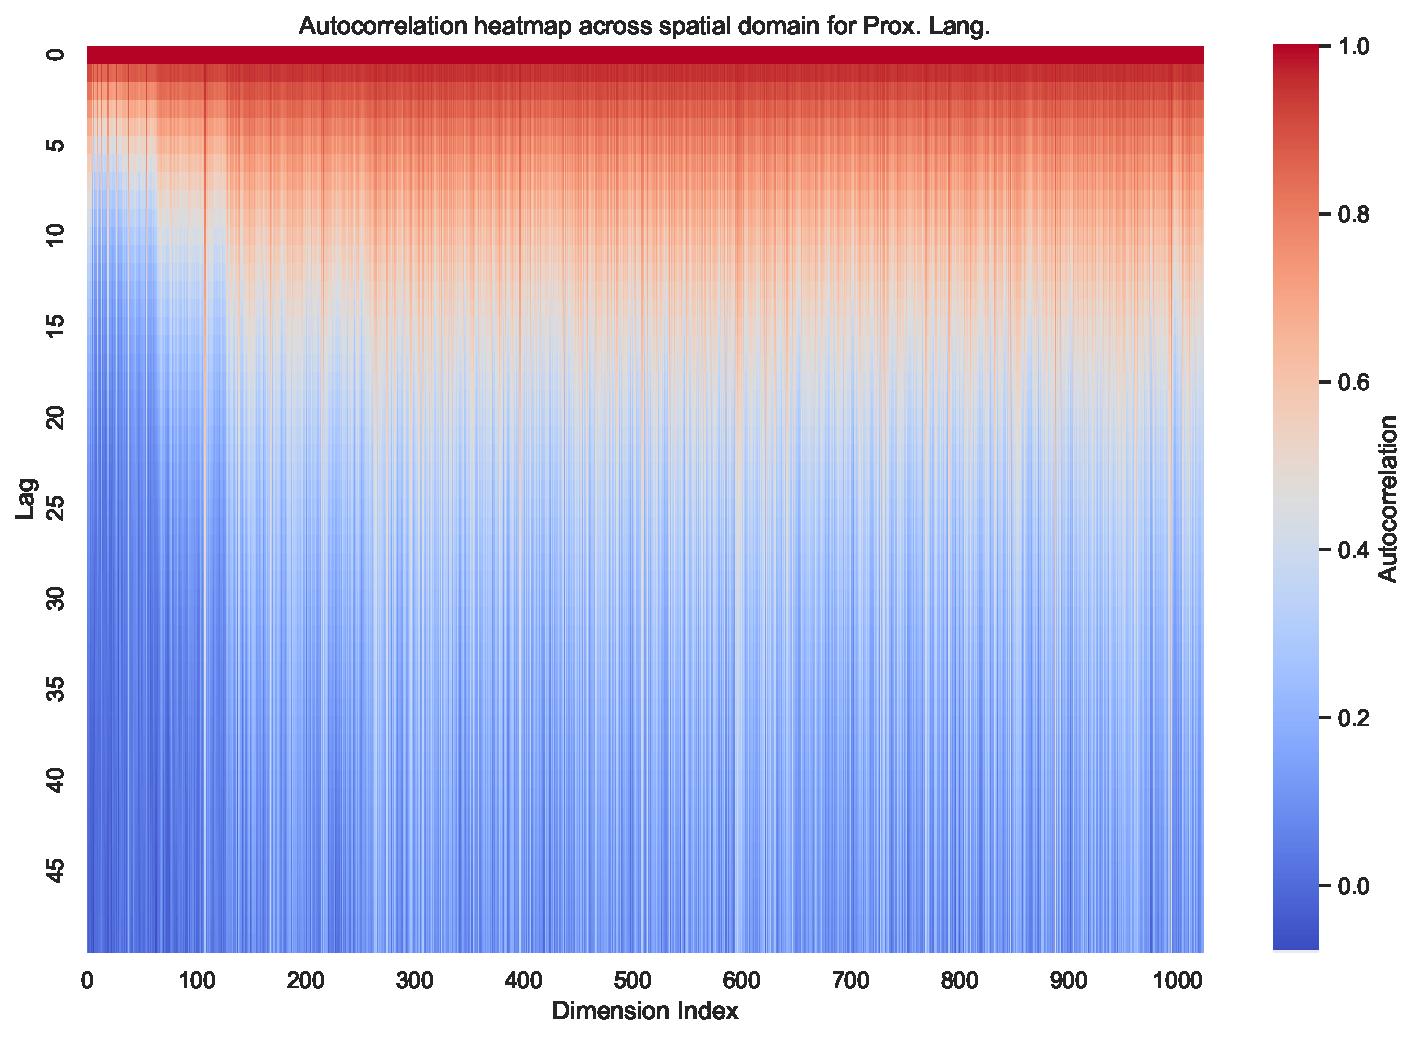
\includegraphics[width=\linewidth]{IMG/haar1d/acf_spatial_haar_Prox. Lang..pdf}
        \caption{Prox. Langevin}
    \end{subfigure}
    \hfill
    \begin{subfigure}{0.45\textwidth}
        \centering
        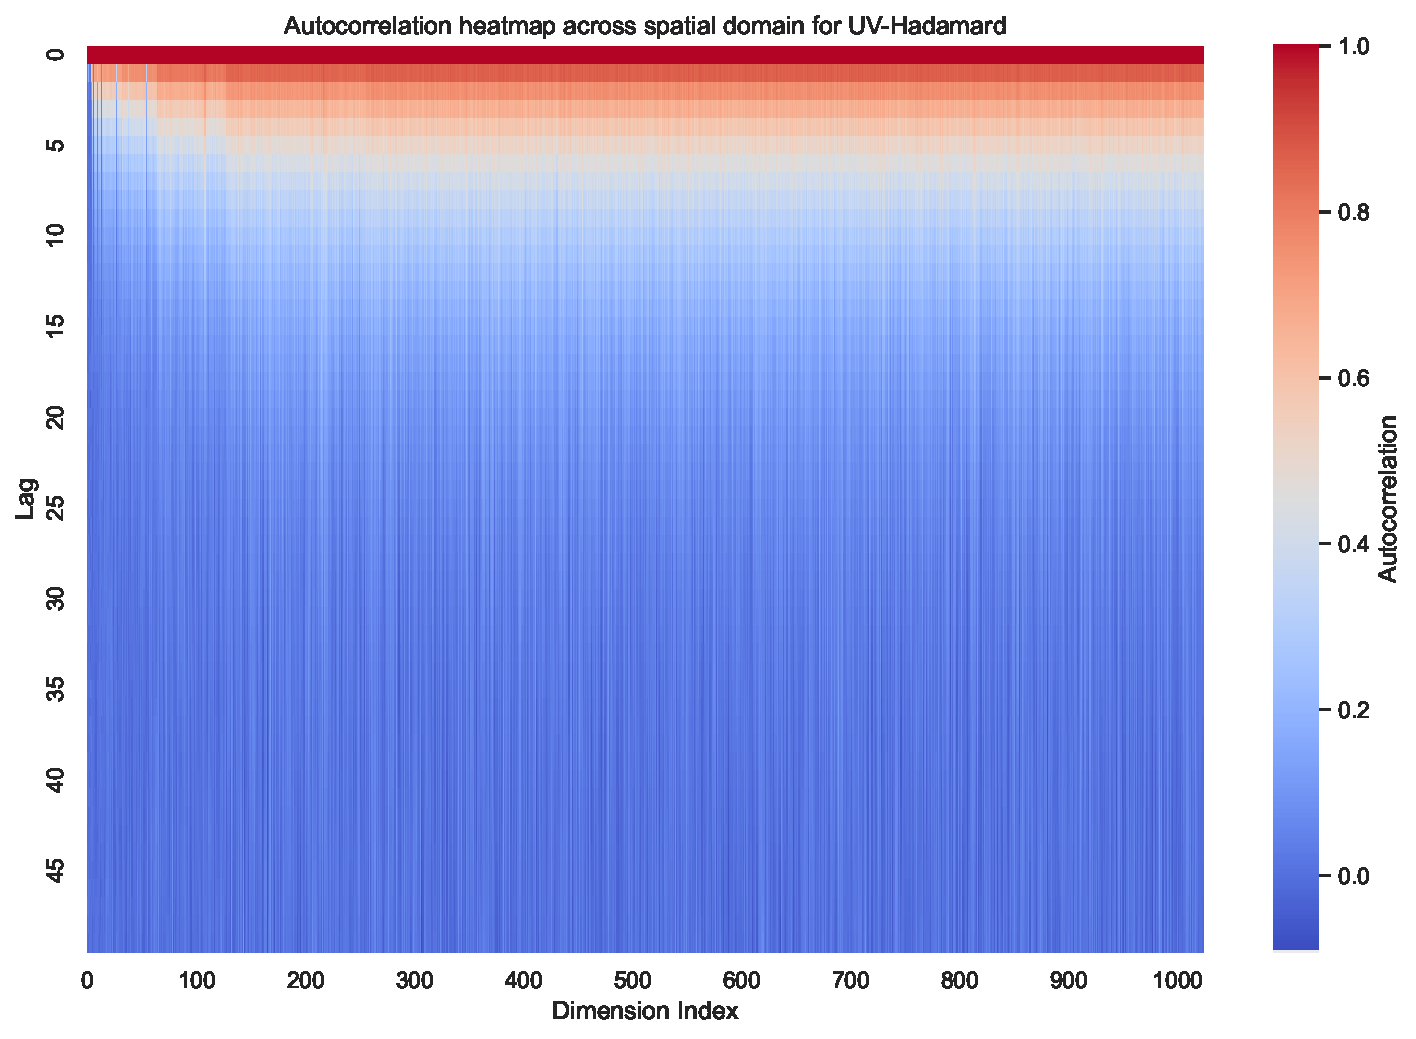
\includegraphics[width=\linewidth]{IMG/haar1d/acf_spatial_haar_UV-Hadamard.pdf}
        \caption{UV-Hadamard}
    \end{subfigure}

    \vspace{0.5cm}

    % Row 2
    \begin{subfigure}{0.45\textwidth}
        \centering
        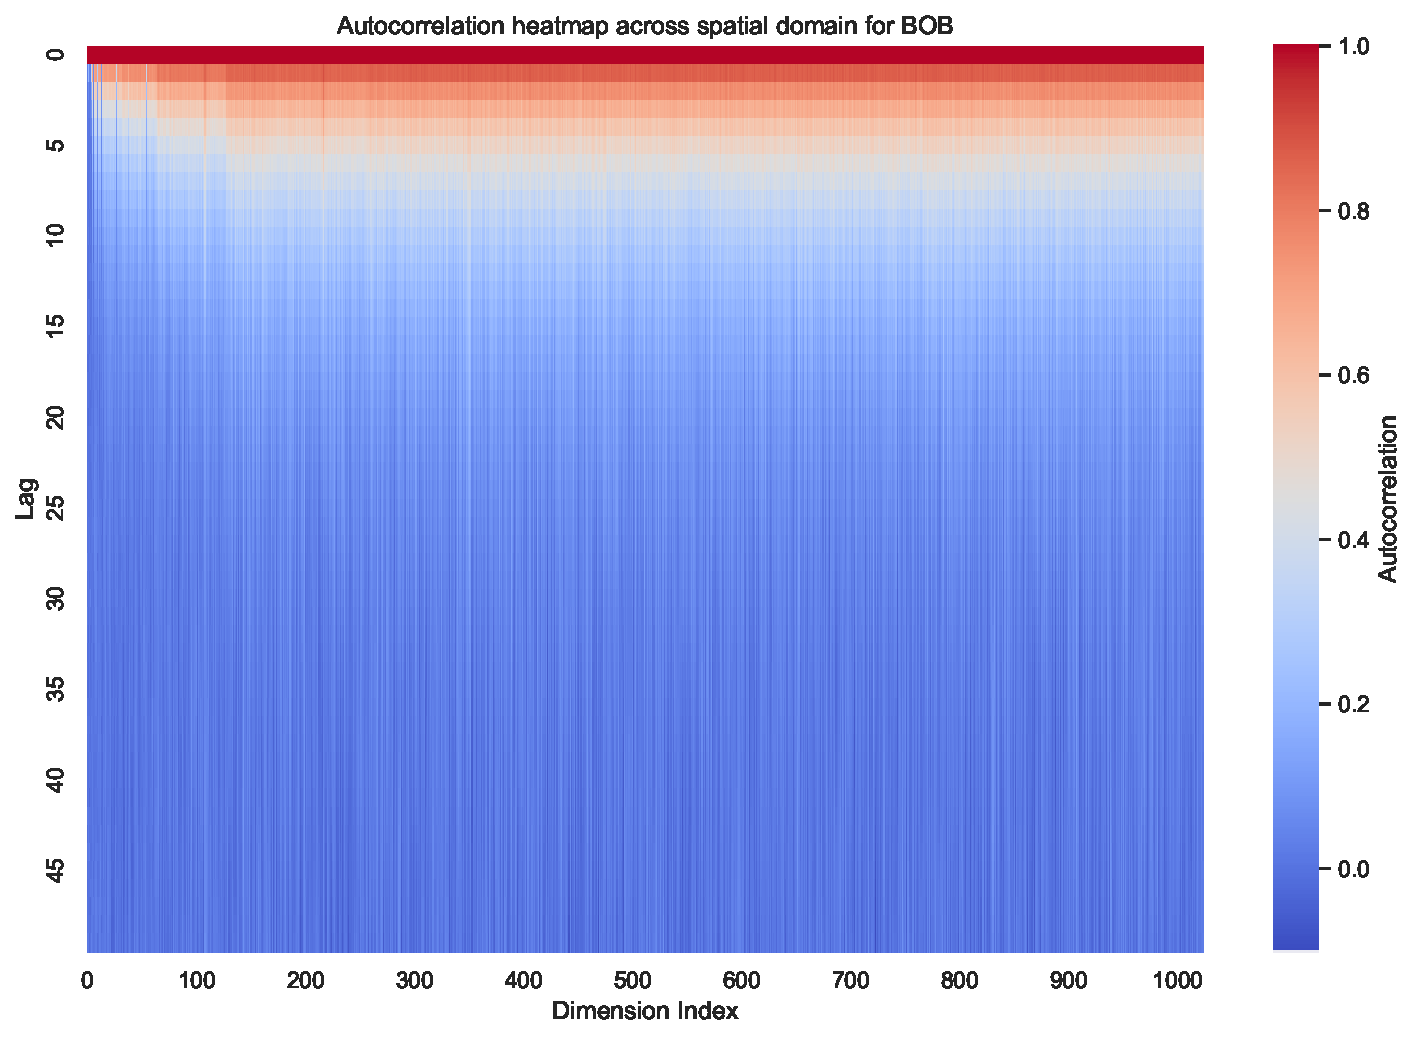
\includegraphics[width=\linewidth]{IMG/haar1d/acf_spatial_haar_BOB.pdf}
        \caption{BOB}
    \end{subfigure}
    \hfill
    \begin{subfigure}{0.45\textwidth}
        \centering
        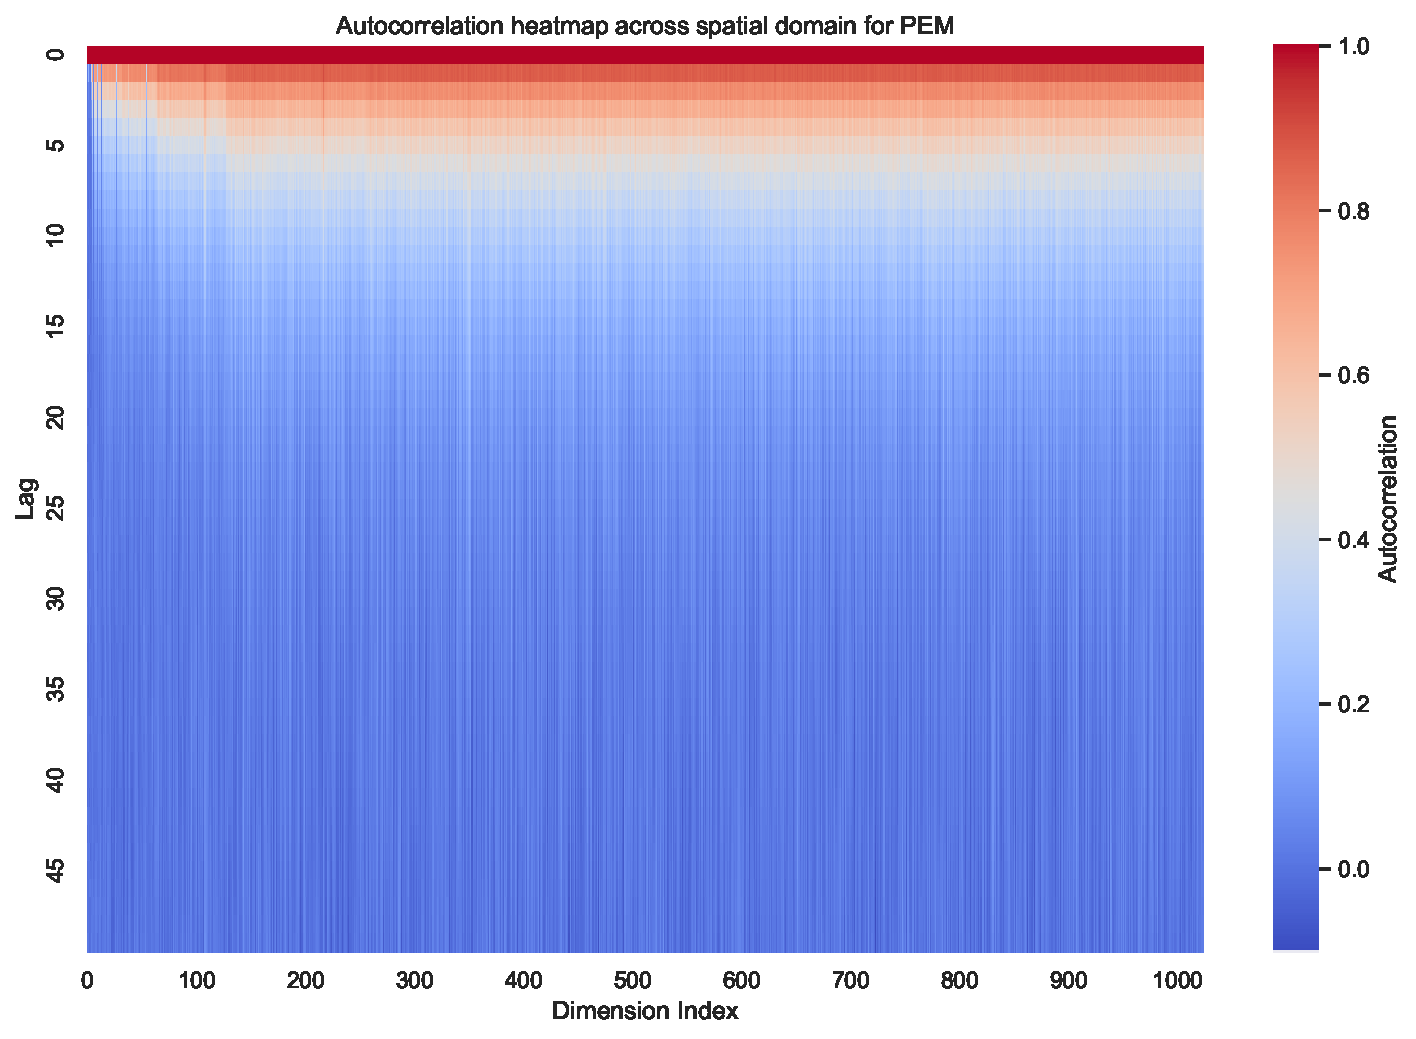
\includegraphics[width=\linewidth]{IMG/haar1d/acf_spatial_haar_PEM.pdf}
        \caption{PEM}
    \end{subfigure}

    \vspace{0.5cm}

    % Row 3
    \begin{subfigure}{0.45\textwidth}
        \centering
        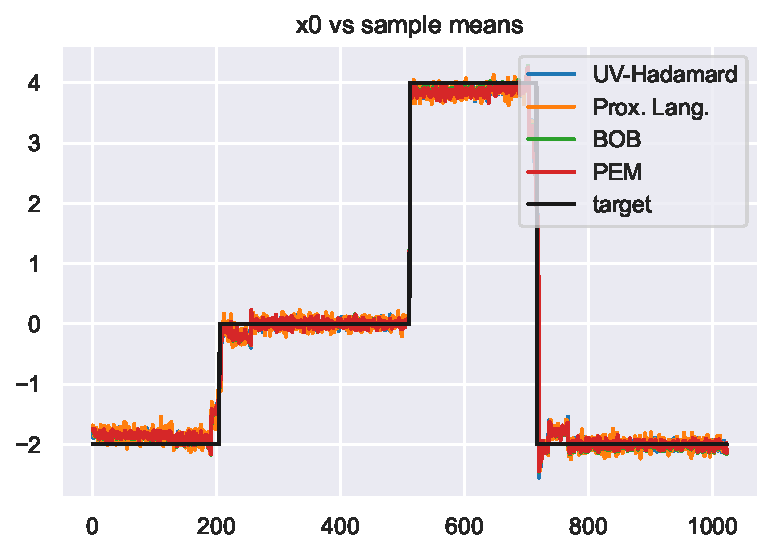
\includegraphics[width=\linewidth]{IMG/haar1d/mean_haar.pdf}
        \caption{Sample Means}
    \end{subfigure}
    \hfill
    \begin{subfigure}{0.45\textwidth}
        \centering
        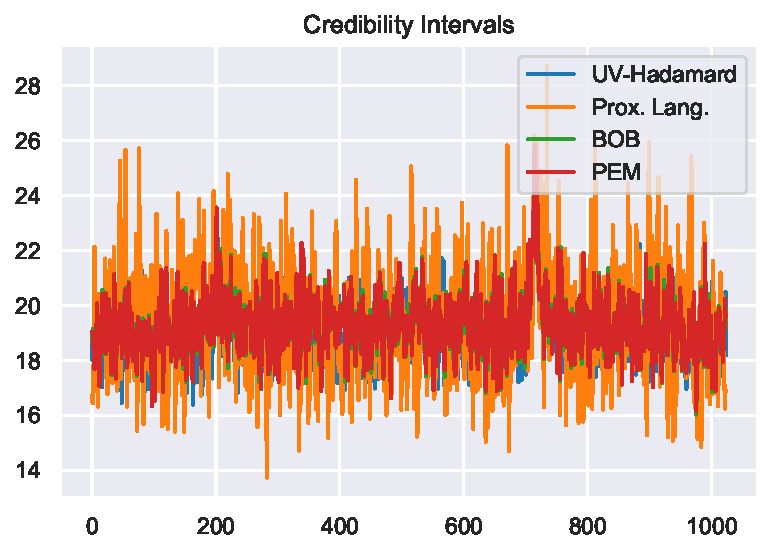
\includegraphics[width=\linewidth]{IMG/haar1d/cred_haar.pdf}
        \caption{Credibility Intervals}
    \end{subfigure}

    \caption{(a)-(d) Heatmap representation of ACF values at various lags for 1024 dimensions; (e) Sample means (f) 90\% Credibility intervals (log-scale)}
    \label{fig:haar_1d}
\end{figure}

\subsection{2D Deconvolution with Haar wavelets}
We perform inpainting: $A = UW^T$, where $U$ is a masking operator and $W$ represents a two-dimensional Haar wavelet transform. We run proximal and Hadamard Langevin, as well as the cartesian schemes, for $\beta = 5,100,500$. All methods are run for 10,000 burn-in iterations and 6000 sampling iterations, with a subsampling frequency of 20 (300 samples total). For the 300 samples we observe the means, as well as the quantile differences. The original, perturbed and MAP recovered images can be seen in Figure \ref{fig:camera_mask}. Furthermore, the means and quantile differences for various $\beta$ can be found in Figures \ref{fig:inpainting2} and \ref{fig:inpainting3}. In general, for small values of $\beta$, the greatest variations occur at the masked pixels. For larger values of $\beta$, we observe the most variance at the image edges.

\begin{figure}[htp]
    \centering
    \begin{subfigure}[b]{0.27\textwidth}
        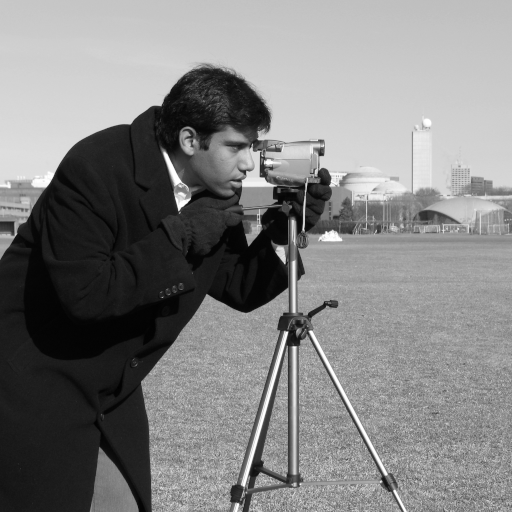
\includegraphics[width=\linewidth]{IMG/haar2d/cameraman.png}
        %\caption{Contact angle with various pseudo dosages}
        \label{fig:cam_orig}
    \end{subfigure}
\hfil 
    \begin{subfigure}[b]{0.3\textwidth}
        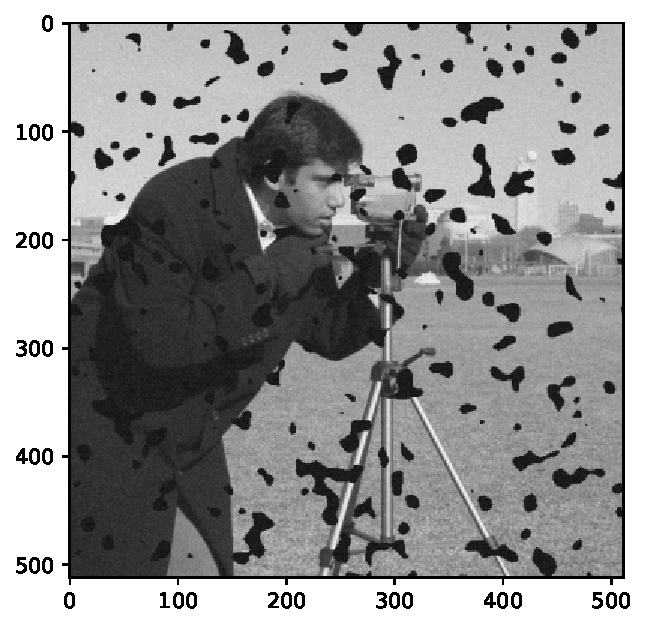
\includegraphics[width=\linewidth]{IMG/haar2d/observation.pdf}
        %\caption{Contact angle with various pseudo dosages}
        \label{fig:cam_obs}
    \end{subfigure}
\hfil
    \begin{subfigure}[b]{0.3\textwidth}
        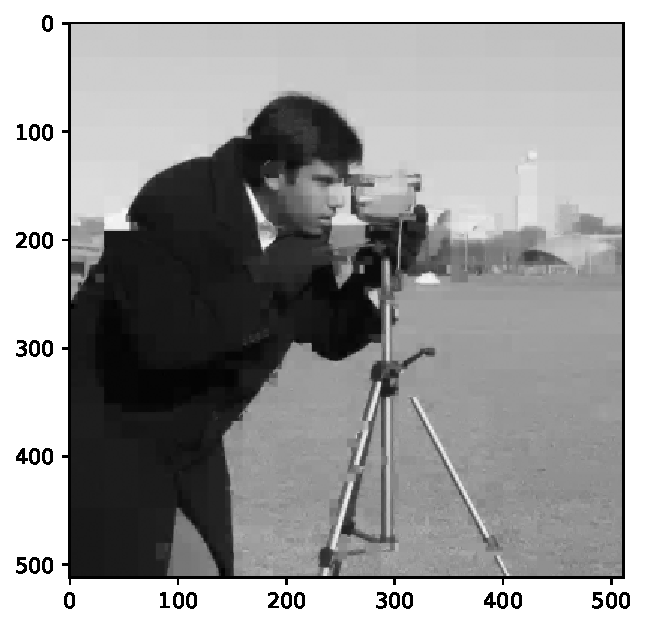
\includegraphics[width=\linewidth]{IMG/haar2d/mode.pdf}
        %\caption{Contact angle with various pseudo dosages}
        \label{fig:cam_mode}
    \end{subfigure}
    \caption{Original, perturbed and MAP recovered image.}\label{fig:camera_mask}
\end{figure}

\begin{figure}[!htp]
    \centering

\begin{tabular}{c@{}c@{}c@{}c@{}c}
&Hadamard&Hadamard&Prox-l1&Prox-l1\\    
&(mean)&(percentile)&(mean)&(percentile)\\
\rotatebox{90}{\hspace{2em}$\beta=5$}&
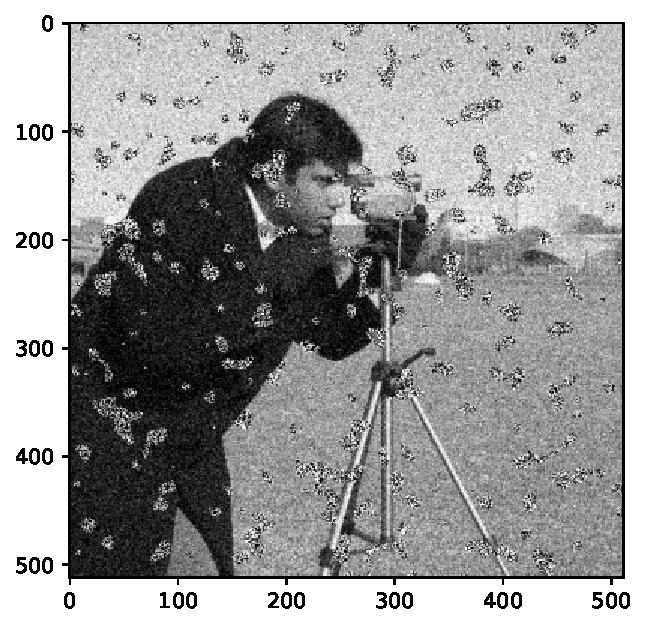
\includegraphics[width=0.21\linewidth]{IMG/haar2d/results-5/uv_mean.pdf}
&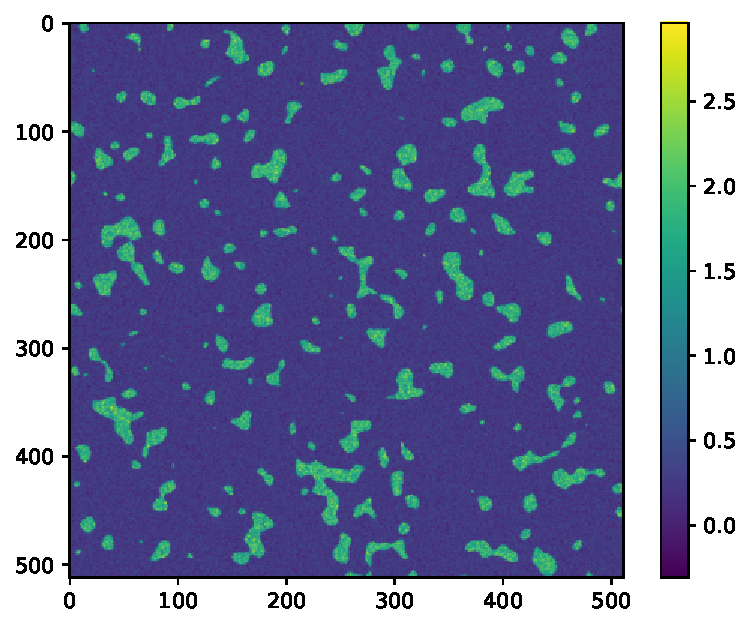
\includegraphics[width=0.25\linewidth]{IMG/haar2d/results-5/uv_percentile.pdf}
&
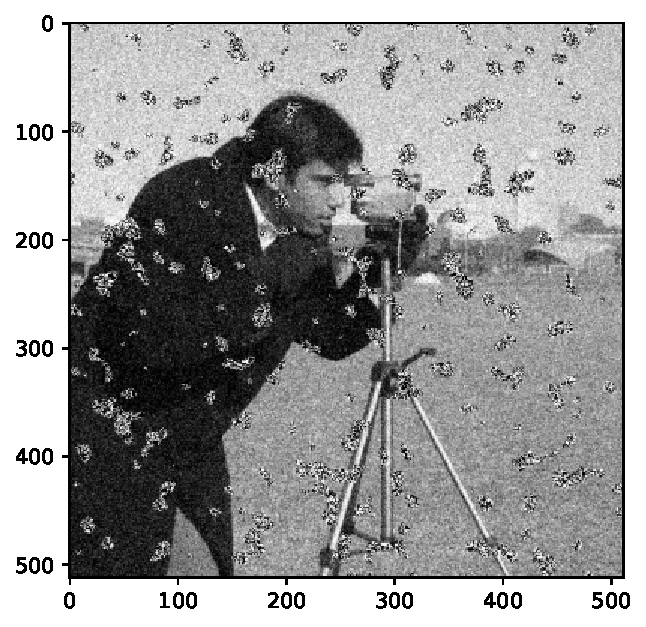
\includegraphics[width=0.21\linewidth]{IMG/haar2d/results-5/prox_mean.pdf}
&
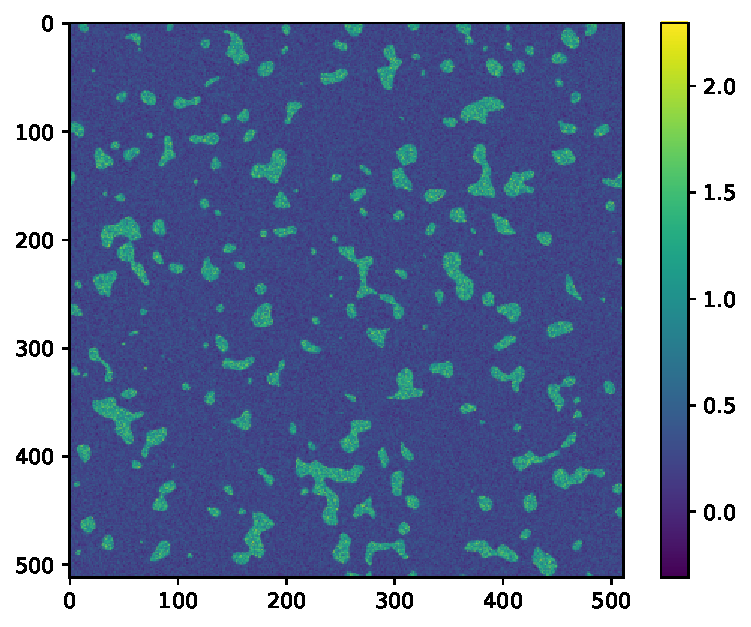
\includegraphics[width=0.25\linewidth]{IMG/haar2d/results-5/prox_percentile.pdf}
\\
\rotatebox{90}{\hspace{2em}$\beta=100$}&
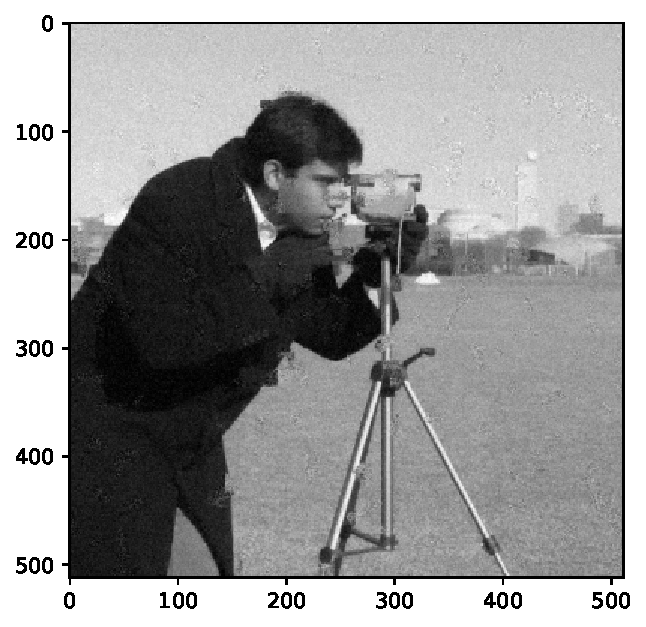
\includegraphics[width=0.21\linewidth]{IMG/haar2d/results-100/uv_mean.pdf}
&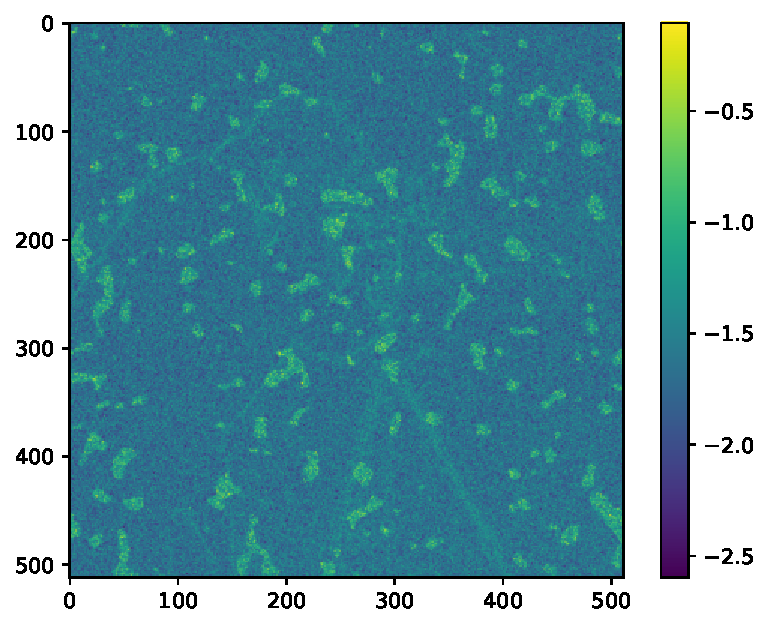
\includegraphics[width=0.25\linewidth]{IMG/haar2d/results-100/uv_percentile.pdf}
&
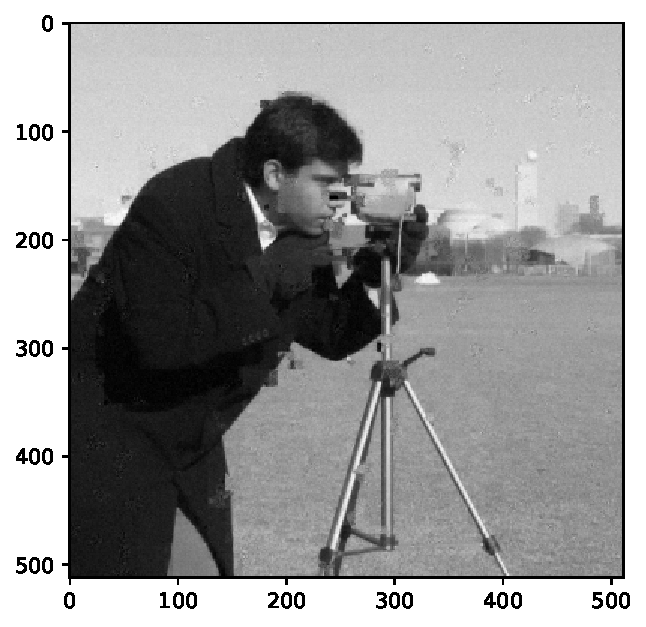
\includegraphics[width=0.22\linewidth]{IMG/haar2d/results-100/prox_mean.pdf}
&
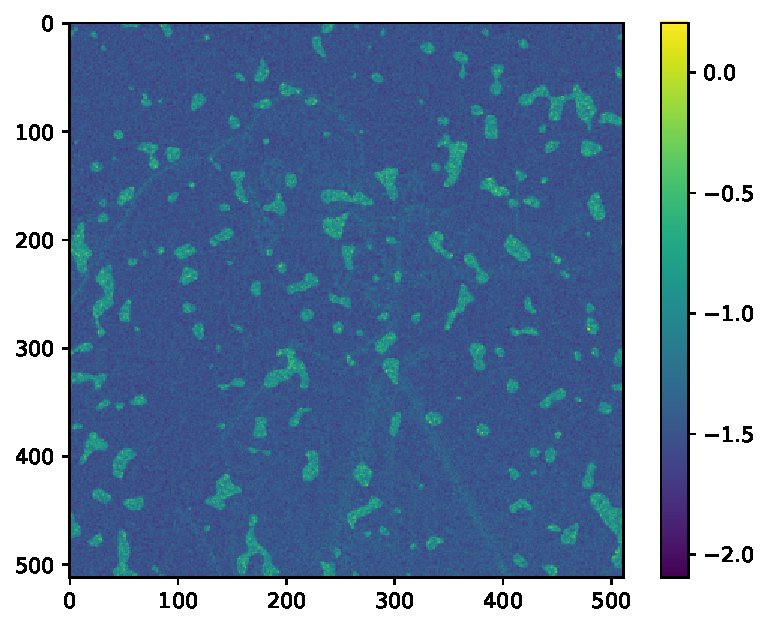
\includegraphics[width=0.25\linewidth]{IMG/haar2d/results-100/prox_percentile.pdf}
\\
\rotatebox{90}{\hspace{2em}$\beta=500$}&
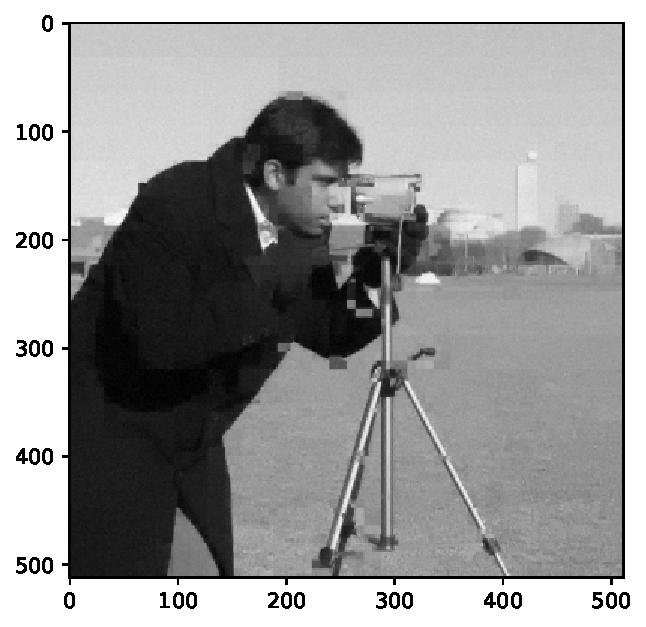
\includegraphics[width=0.21\linewidth]{IMG/haar2d/results-500/uv_mean.pdf}
&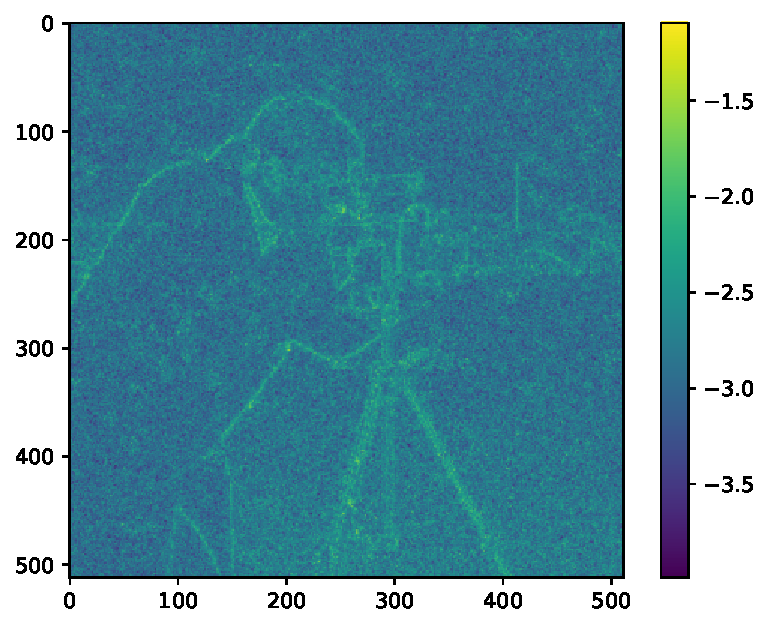
\includegraphics[width=0.25\linewidth]{IMG/haar2d/results-500/uv_percentile.pdf}
&
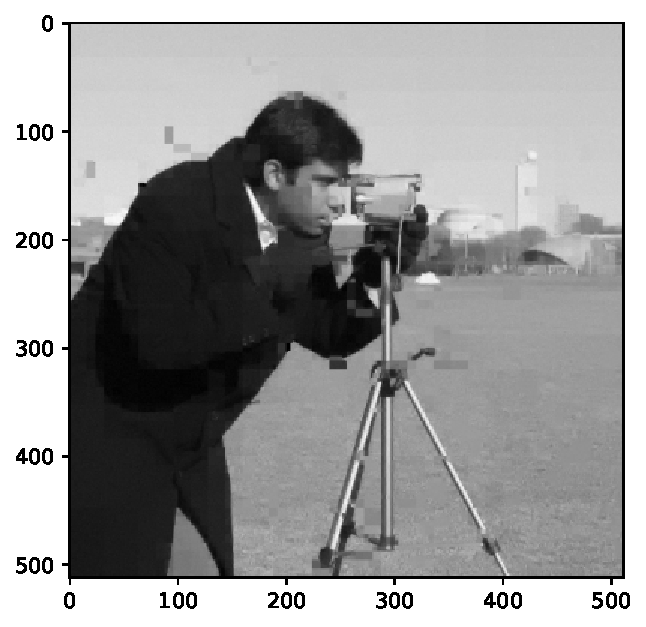
\includegraphics[width=0.21\linewidth]{IMG/haar2d/results-500/prox_mean.pdf}
&
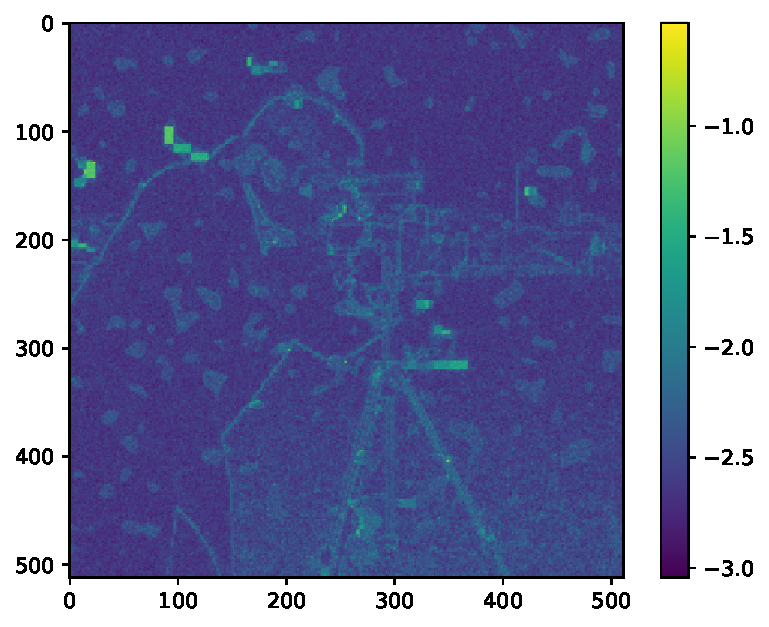
\includegraphics[width=0.25\linewidth]{IMG/haar2d/results-500/prox_percentile.pdf}
\end{tabular}    
    \caption{UV and Prox Hadamard: Mean images and  log differences between 95 and 5 quantiles for different choices of $\beta$.}
    \label{fig:inpainting2}
\end{figure}

\begin{figure}[!htp]
    \centering

\begin{tabular}{c@{}c@{}c@{}c@{}c}
&Hadamard&Hadamard&Prox-l1&Prox-l1\\    
&(mean)&(percentile)&(mean)&(percentile)\\
\rotatebox{90}{\hspace{2em}$\beta=5$}&
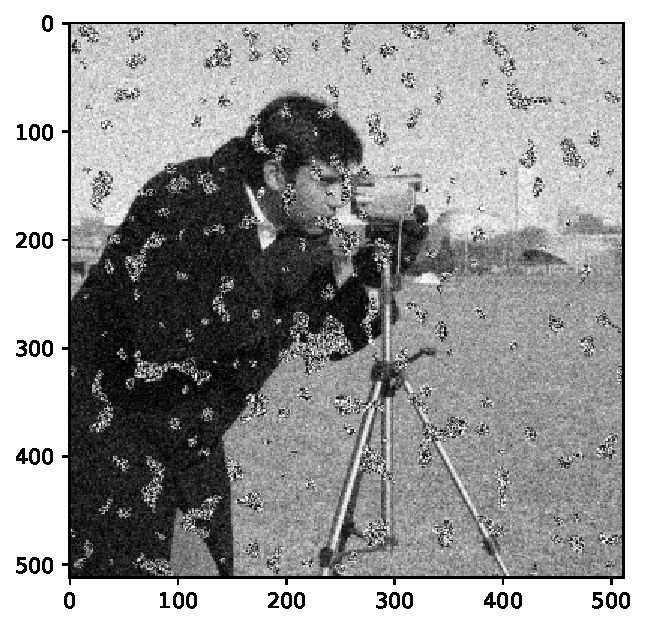
\includegraphics[width=0.21\linewidth]{IMG/haar2d/results-5/bob_mean.pdf}
&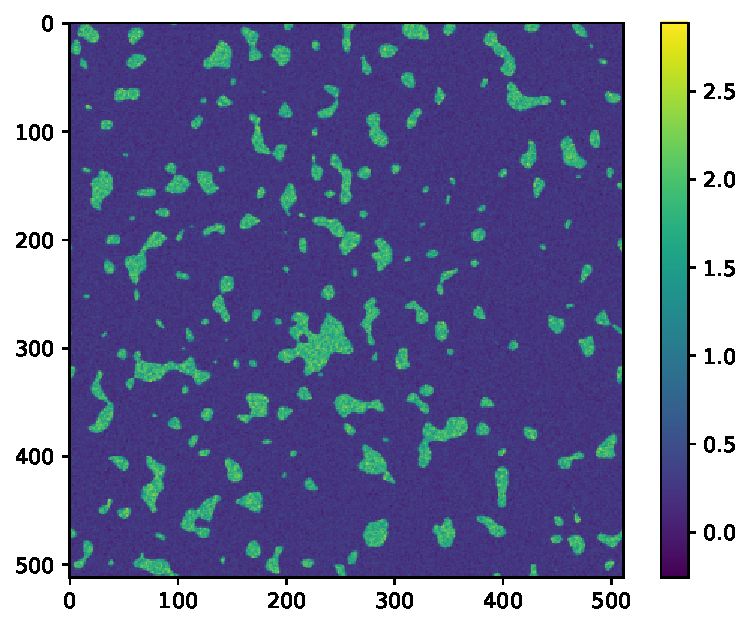
\includegraphics[width=0.25\linewidth]{IMG/haar2d/results-5/bob_percentile.pdf}
&
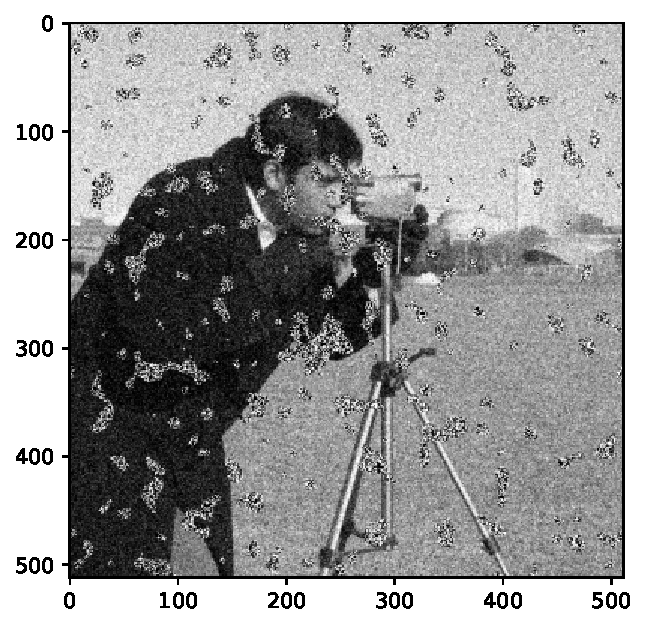
\includegraphics[width=0.21\linewidth]{IMG/haar2d/results-5/pem_mean.pdf}
&
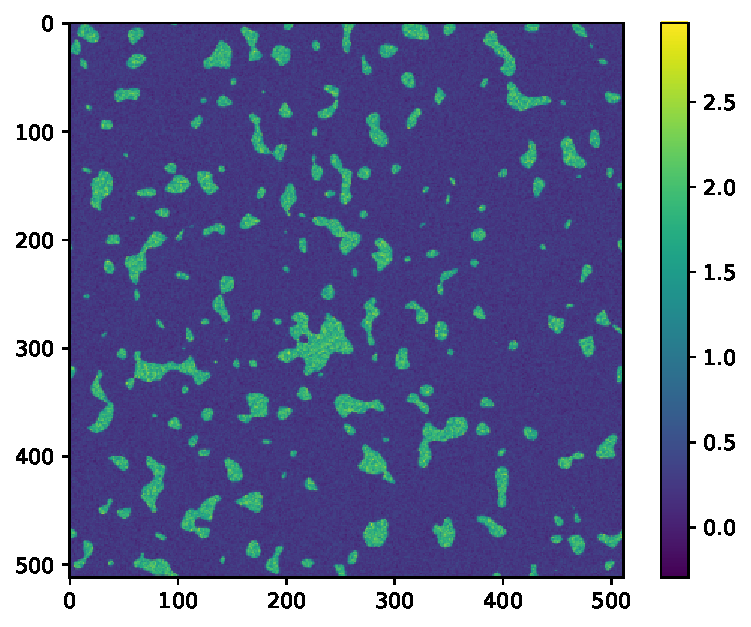
\includegraphics[width=0.25\linewidth]{IMG/haar2d/results-5/pem_percentile.pdf}
\\
\rotatebox{90}{\hspace{2em}$\beta=100$}&
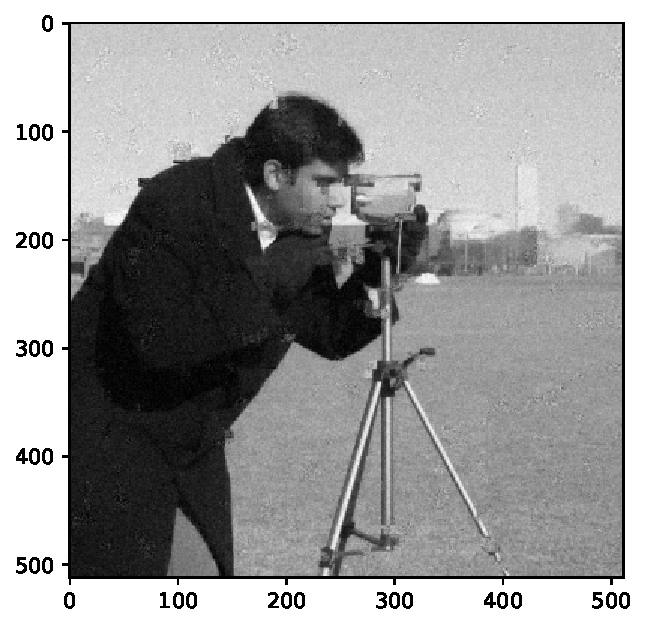
\includegraphics[width=0.21\linewidth]{IMG/haar2d/results-100/bob_mean.pdf}
&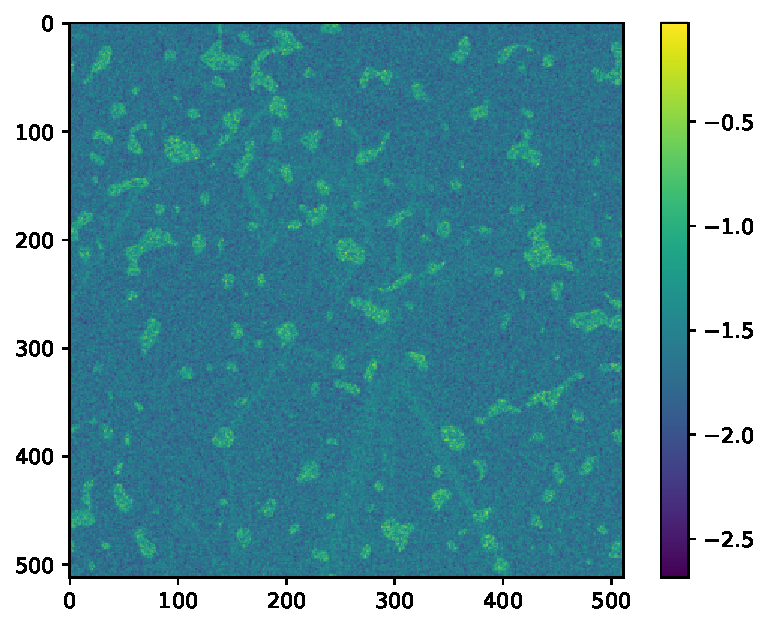
\includegraphics[width=0.25\linewidth]{IMG/haar2d/results-100/bob_percentile.pdf}
&
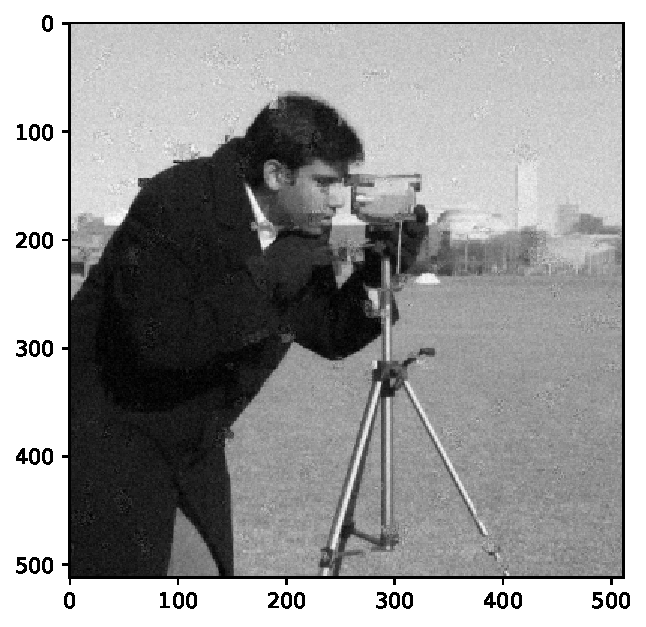
\includegraphics[width=0.22\linewidth]{IMG/haar2d/results-100/pem_mean.pdf}
&
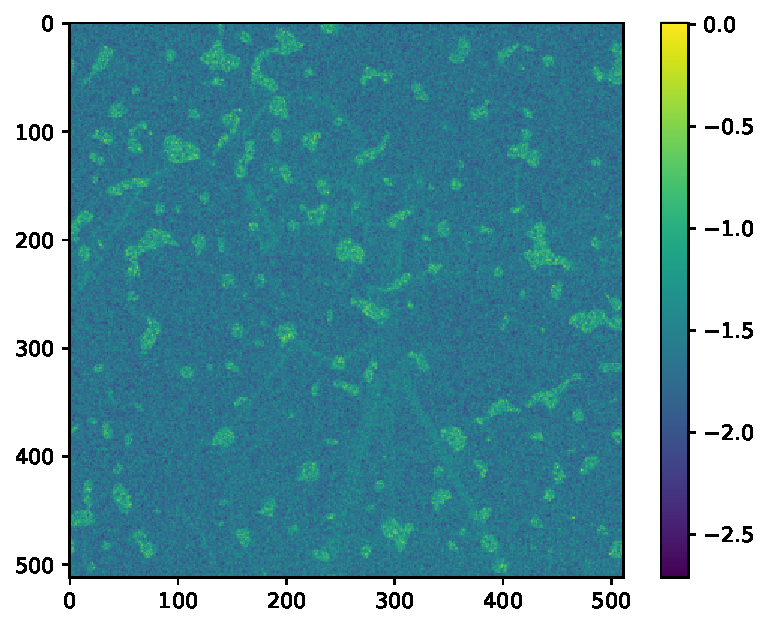
\includegraphics[width=0.25\linewidth]{IMG/haar2d/results-100/pem_percentile.pdf}
\\
\rotatebox{90}{\hspace{2em}$\beta=500$}&
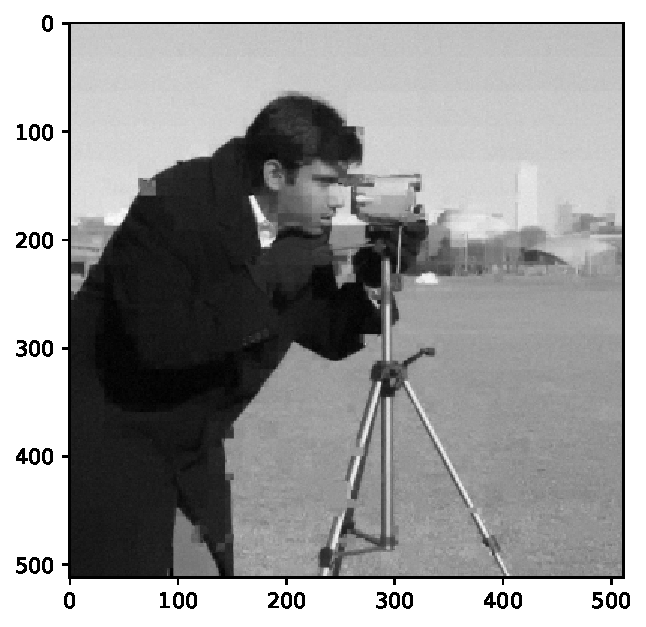
\includegraphics[width=0.21\linewidth]{IMG/haar2d/results-500/bob_mean.pdf}
&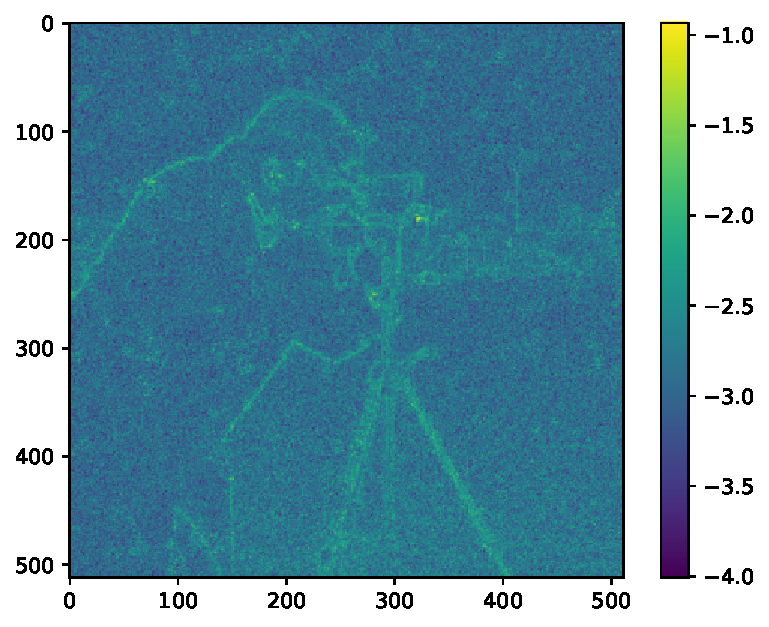
\includegraphics[width=0.25\linewidth]{IMG/haar2d/results-500/bob_percentile.pdf}
&
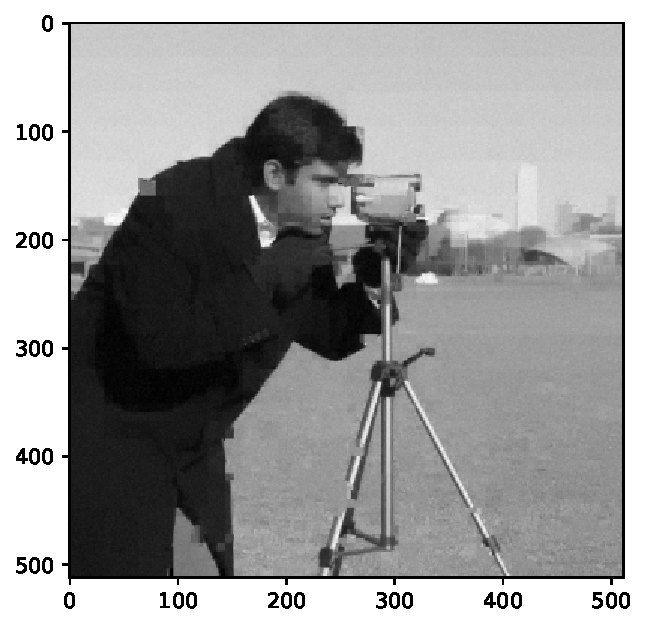
\includegraphics[width=0.21\linewidth]{IMG/haar2d/results-500/pem_mean.pdf}
&
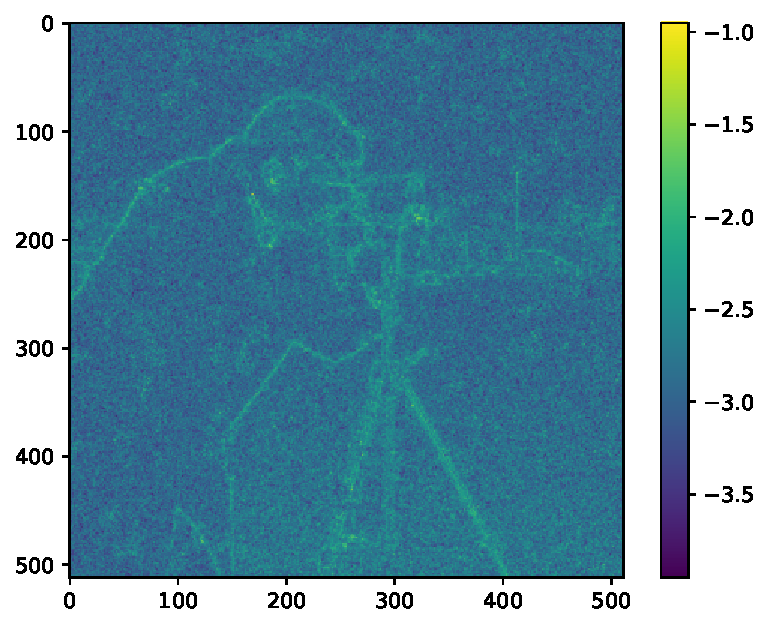
\includegraphics[width=0.25\linewidth]{IMG/haar2d/results-500/pem_percentile.pdf}
\end{tabular}    
    \caption{Cartesian BOB and PEM: Mean images and  log differences between 95 and 5 quantiles for different choices of $\beta$.}
    \label{fig:inpainting3}
\end{figure}
\newpage
\subsection{Summary}
Across regression, classification, and inverse problems, our experiments demonstrate that Hadamard Langevin offers competitive sampling performance, with efficiency close to Gibbs in moderate dimensions and improvements over Cartesian schemes in deconvolution tasks. In the one-dimensional regression problem, PEM showed the best numerical accuracy, though its behaviour was obscured by Monte Carlo error at small stepsizes. For high-dimensional regression and classification, deterministic Lasso consistently matched or outperformed Bayesian samplers in predictive accuracy, while the latter offered comparable ROC/AUC scores without clear gains. By contrast, in inverse problems such as deconvolution and inpainting, Bayesian samplers provided meaningful uncertainty quantification, with variance correctly concentrated near discontinuities, masked regions, and edges, and Hadamard and related schemes yielding stable reconstructions. Taken together, these results suggest that Hadamard Langevin is a promising alternative to sampling methods such as Gibbs in moderate-dimensional problems.

\part{Hyperparameter Optimization}

\chapter{Stocbio, StocHOAG and the conditioning issue} \label{chp: stoc_cond}
\section{Introduction}
In the field of smooth bilevel optimization, existing deterministic algorithms, based on implicit differentiation of the inner problem, such as HOAG \cite{pedregosa2016hyperparameter} and BA \cite{ghadimi2018approximation}, have been effectively used to solve problems in areas such as hyperparameter optimization. These algorithms, however, exhibit a high per-iteration complexity, in large part due to the inversion of a matrix, that takes place during the implicit differentiation stage. To tackle this issue, stochastic algorithms have been developed. Here, stochasticity is introduced in large part to invert the Hessian in sub-$\mathcal{O}(n^3)$ time. We will be investigating one such algorithm in partiular - stocBio \cite{ji2021bilevel}. This algorithm, albeit having one of the fastest convergence rates among comparable algorithms, requires the tuning of a large number of parameters. Furthermore, stocBio suffers from a sensitivity to the conditioning of the inner problem, much like most other bilevel algorithms. The aim of this report is to investigate a different parameter setup for the algorithm that alleviates this sensitivity.
%\begin{thebibliography}{99}

\subsection{Problem Statement \& Assumptions}
We set up a bilevel problem. For a bounded domain $\mathcal D \subset \mathbb{R}^r$, we wish to find $\lambda \in \mathcal{D}$ and $\hat{x}(\lambda) \in \mathbb{R}^n$, such that
\begin{align} 
&\min_{\lambda \in \mathcal{D}} \mathcal{L}\left(\lambda \right) \triangleq C(\hat{x}(\lambda), \lambda) \label{outer_hoag_neu}\\
&\text { s.t. } \hat{x}(\lambda) =\underset{x \in \mathbb{R}^{n}} \argmin {F(x, \lambda)}. \label{inner_hoag_neu}
\end{align}
\begin{comment}
    We will denote the sampled terms as follows. For i.i.d. samples $\zeta, \xi$, uniformly randomly selected from the given data $\{\zeta_i, \xi_j, i = 1,\hdots, m_1; j = 1,\hdots, m_2 \}$, we have:
\begin{align*}
    \mathbb{E}_{\zeta}[\tilde{F}\left(x, \lambda ; \zeta\right)] &= F\left(x, \lambda\right) \\
    \mathbb{E}_{\xi}[\tilde{C}(x,\lambda,\xi)] &= C(x,\lambda) \\
    %\mathbb{E}_{\theta}[\nabla_\lambda \tilde{C}(x_k,\lambda_k,\theta)] &= \nabla_\lambda \tilde{C}(x_k,\lambda_k) \\
    %\mathbb{E}_{\kappa}[\nabla_{x \lambda}^2 \tilde{F}(x_k,\lambda_k,\kappa)] &= \nabla_{x \lambda}^2 \tilde{F}(x_k,\lambda_k)
\end{align*}

For a function $f:\mathbb{R}^n \xrightarrow[]{} \mathbb{R}$, will denote the conditional expectation $\mathbb{E}_{x_k} [f(x)] = \mathbb{E}[f(x) | x = x_k].$ We introduce some standard assumptions that we will need to tackle this problem.
\end{comment}

% --- Bridge paragraph ---
In many practical applications, the functions $F$ and $C$ are defined as averages over large datasets. 
Computing the exact gradients or Hessians can therefore be prohibitively expensive, especially in high-dimensional settings. 
To alleviate this computational burden, we introduce stochastic approximations, where gradients and function values are computed using randomly sampled subsets of the data. 

Formally, let $\{\zeta_i\}_{i=1}^{m_1}$ and $\{\xi_j\}_{j=1}^{m_2}$ denote the datasets associated with $F$ and $C$, respectively. 
We define the stochastic approximations $\tilde{F}(x, \lambda; \zeta)$ and $\tilde{C}(x, \lambda; \xi)$ as unbiased estimators of $F$ and $C$:
\begin{align*}
    \mathbb{E}_{\zeta}[\tilde{F}\left(x, \lambda ; \zeta\right)] &= F\left(x, \lambda\right), \\
    \mathbb{E}_{\xi}[\tilde{C}(x,\lambda,\xi)] &= C(x,\lambda),
\end{align*}
where $\zeta$ and $\xi$ are drawn uniformly at random from their respective datasets.



\begin{assumption}[Convexity] \label{conv_ass}
    The inner function $F(x, \lambda)$ is $\mu$ strongly-convex w.r.t. $x$.
\end{assumption}

\begin{assumption}[Smoothness] \label{smo_ass}
Let $(x,\lambda) \in \mathbb{R}^{n} \times \mathcal{D}$. The loss function $C(x,\lambda)$ and $F(x,\lambda)$ satisfy the following smoothness assumptions:
\begin{itemize}
    \item The function $C(x,\lambda)$ is $M$-Lipschitz, i.e., for any $(x,\lambda), (x^{\prime},\lambda^{\prime}) \in \mathbb{R}^{n} \times \mathcal{D}$,
$$
\left|C(x,\lambda)-C(x^{\prime},\lambda^{\prime})\right| \leq M\left\|(x,\lambda)-(x^{\prime},\lambda^{\prime})\right\| .
$$
    \item $\nabla C(x,\lambda)$ and $\nabla F(x,\lambda)$ are L-Lipschitz, i.e., for any $(x,\lambda), (x^{\prime},\lambda^{\prime}) \in \mathbb{R}^{n} \times \mathcal{D}$,
$$
\begin{aligned}
\left\|\nabla C(x,\lambda)-\nabla C(x^{\prime},\lambda^{\prime})\right\| & \leq L\left\|(x,\lambda)-(x^{\prime},\lambda^{\prime})\right\|, \\
\left\|\nabla F(x,\lambda)-\nabla F(x^{\prime},\lambda^{\prime})\right\| & \leq L\left\|(x,\lambda)-(x^{\prime},\lambda^{\prime})\right\| .
\end{aligned}
$$
\end{itemize}
For the stochastic case, the same assumptions hold for $C(x,\lambda ; \xi)$ and $F(x,\lambda, \zeta)$ for any given $\xi$ and $\zeta$.
\end{assumption}

An immediate consequence of the previous assumption are bounds on the variances of various sampled gradients:
\begin{proposition}[Bounded variance of $\nabla \tilde{C}, \nabla_{x\lambda}^2 \tilde{F},\nabla_{xx}^2 \tilde{F}$. Lemma 1 in \cite{ji2021bilevel}] \label{boun_var}
    Suppose, Assumption \ref{smo_ass} holds. Then for any $x,\lambda,\zeta$,
    \begin{align*}
        &\mathbb{E}_\zeta \|\nabla \tilde{C}(x,\lambda,\zeta) - \nabla C(x,\lambda)\|^2 \leq M^2 \\
        &\mathbb{E}_\zeta \|\nabla_{x\lambda}^2 \tilde{F}(x,\lambda,\zeta) - \nabla_{x\lambda}^2 F(x,\lambda)\|^2 \leq L^2 \\
        &\mathbb{E}_\zeta \|\nabla_{xx}^2 \tilde{F}(x,\lambda,\zeta) - \nabla_{xx}^2 F(x,\lambda)\|^2 \leq L^2 
    \end{align*}
\end{proposition}

\begin{comment}
    \begin{assumption}[Partial Lipschitz Smoothness] \label{pls_ass}
Let $z = (x,\lambda) \in \mathbb{R}^{n} \times \mathcal{D}$. Suppose the derivatives $\nabla_{x\lambda} F(z)$ and $\nabla_x^2 F(z)$ are $\tau$ - and $\rho$ - Lipschitz, i.e.,
- For any $z, z^{\prime},\left\|\nabla_{x\lambda} F(z)-\nabla_{x\lambda} F(z^{\prime})\right\| \leq \tau\left\|z-z^{\prime}\right\|$.
- For any $z, z^{\prime},\left\|\nabla_x^2 F(z)-\nabla_x^2 F\left(z^{\prime}\right)\right\| \leq \rho\left\|z-z^{\prime}\right\|$.
For the stochastic case, the same assumptions hold for $\nabla_{x\lambda} F(z; \zeta)$ and $\nabla_x^2 F(z ; \zeta)$ for any $\zeta$.
\end{assumption}

\subsection{stocBio and stoc-HOAG}
We begin by introducing the algorithm introduced by Ji et al. that can be used to tackle problem (\ref{outer_hoag_neu}-\ref{inner_hoag_neu}) \cite{ji2021bilevel}. Firstly, we define some of the relevant parameters:
\begin{itemize}
        \item $S$ - the number of samples in every inner SGD step
        \item $D$ - The number of SGD iterations required every time the inner problem is solved.
        \item $D_g$ - the number of samples of $\nabla_{x\lambda} \tilde{F}$ (for every approximate hypergradient).
        \item $D_f$ - The number of samples of $\nabla_x \tilde{C}$ (for every approximate hypergradient).
        \item $\mathcal{S}_{\nabla_\lambda C}$ - the number of samples of $\nabla_{\lambda} \tilde{C}$ (for every approximate hypergradient).
        \item $B$ - The base number of samples of $\nabla_{xx} \tilde{F}$ for the neumann series (\ref{HIA_stocBio}), where the number of samples at the $Q+1-j$-th step of the subroutine is $BQ(1-\eta\mu)^{j-1}.$
    \end{itemize}
Note that the parameters for stocBio are set up in a global manner - at any point during the runtime these are fixed. The Neumann series and its sampling will be explained in section \ref{neumann_series}. The algorithm is described in \ref{alg:stocbio}.
\end{comment}

% --- reformat

\begin{assumption}[Partial Lipschitz Smoothness] \label{pls_ass}
Let $z = (x,\lambda) \in \mathbb{R}^{n} \times \mathcal{D}$. Suppose the derivatives $\nabla_{x\lambda} F(z)$ and $\nabla_x^2 F(z)$ satisfy the following Lipschitz conditions:
\begin{itemize}
    \item For any $z, z^{\prime}$, $\left\|\nabla_{x\lambda} F(z)-\nabla_{x\lambda} F(z^{\prime})\right\| \leq \tau\left\|z-z^{\prime}\right\|$.
    \item For any $z, z^{\prime}$, $\left\|\nabla_x^2 F(z)-\nabla_x^2 F\left(z^{\prime}\right)\right\| \leq \rho\left\|z-z^{\prime}\right\|$.
\end{itemize}
For the stochastic case, the same assumptions hold for $\nabla_{x\lambda} F(z; \zeta)$ and $\nabla_x^2 F(z ; \zeta)$ for any $\zeta$.
\end{assumption}

\subsection{stocBio and stoc-HOAG}
We begin by introducing the algorithm introduced by Ji et al. that can be used to tackle problem (\ref{outer_hoag_neu}-\ref{inner_hoag_neu}) \cite{ji2021bilevel}. Firstly, we define some of the relevant parameters:
\begin{itemize}
    \item $S$: number of samples in every inner SGD step.
    \item $D$: number of SGD iterations required each time the inner problem is solved.
    \item $D_g$: number of samples of $\nabla_{x\lambda} \tilde{F}$ for each approximate hypergradient.
    \item $D_f$: number of samples of $\nabla_x \tilde{C}$ for each approximate hypergradient.
    \item $\mathcal{S}_{\nabla_\lambda C}$: number of samples of $\nabla_{\lambda} \tilde{C}$ for each approximate hypergradient.
    \item $B$: base number of samples of $\nabla_{xx} \tilde{F}$ for the Neumann series (\ref{HIA_stocBio}), where the number of samples at the $(Q+1-j)$-th step of the subroutine is $BQ(1-\eta\mu)^{j-1}$.
\end{itemize}
Note that the parameters for stocBio are set up in a global manner - at any point during the runtime these are fixed. The Neumann series and its sampling will be explained in section \ref{neumann_series}. The algorithm is described in \ref{alg:stocbio}.



\begin{algorithm}[]
\caption{stocBio \cite{ji2021bilevel}}
\label{alg:stocbio}
\DontPrintSemicolon
\KwIn{Outer stepsize $\nu_k$, Neumann length $Q_k$, parameter $\eta$, inner steps $T_k$}
\For{$k = 1, 2, \dots$}{
    Sample batches $D_f$, $\mathcal{S}_{\nabla_\lambda C}$, $D_g$, $\mathcal{B}_j$\;
    Perform $T_k$ steps of SGD on the inner problem with stepsize $\alpha$, yielding $x_k$\;
    Compute Neumann vector:
    \[
    v_Q = \eta \sum_{q=-1}^{Q_k-1} \prod_{j=Q_k - q}^{Q_k} \left(I - \eta \nabla_{xx}^2 \tilde{F}(x_k, \lambda_k; \mathcal{B}_j)\right) \nabla_x \tilde{C}(x_k, \lambda_k, D_f)
    \]
    Compute stochastic gradient:
    \[
    \widehat{\nabla} \mathcal{L}(\lambda_k) = \nabla_\lambda \tilde{C}(x_k, \lambda_k, \mathcal{S}_{\nabla_\lambda C}) - \left( \nabla_{x \lambda}^2 \tilde{F}(x_k, \lambda_k, D_g) \right)^\top v_Q
    \]
    Update hyperparameters:
    \[
    \lambda_{k+1} = \lambda_k - \nu_k \widehat{\nabla} \mathcal{L}(\lambda_k)
    \]
}
\end{algorithm}


The authors also provide theoretical convergence guarantees for this algorithm.
\begin{theorem}[Theorem 3 in \cite{ji2021bilevel}] \label{thm3}
    Suppose assumptions \ref{conv_ass}-\ref{pls_ass} hold. Let $L_{\mathcal{L}(\lambda_k)} = L + \frac{2L^2 + \tau M^2}{\mu} + \frac{\rho L M + L^3 + \tau M L}{\mu^2} + \frac{\rho L^2 M}{\mu^3} = \mathcal{O}(1/\mu^3)$, choose the outer stepsize $\beta$ as $\frac{1}{4 L_\Phi} = \mathcal{O}(\mu^3), \eta < 1/L$, number of inner steps $D \geq \mathcal{O}(\frac{1}{\mu} \log{\frac{1}{\mu}})$. Then
    \[\frac{1}{K} \sum_{k=0}^{K-1} \mathbb{E} \|\nabla \mathcal{L}(\lambda_k)\|^2 \leq \mathcal{O}\left( \frac{L_{\mathcal{L}}}{K} + \frac{L^2(1-\eta \mu)^2Q}{\mu^2} + \frac{L^5 \sigma^2}{\mu^5 S} + \frac{L^2}{\mu^2 D_g} + \frac{L^2}{\mu^2 D_f} + \frac{L^2}{
    \mu^2 B} \right).\]
    
\end{theorem}
Of note here is that, for small $\mu$, the above is bounded as $\mathcal{O}(1/\mu^5)$. As mentioned previously, our aim will be to change the parameter choices in such a manner, that convergence will be less sensitive to an ill-conditioned problem. For this purpose, we will allow the parameters to change with the outer iteration. As such, we relabel them accordingly


\begin{itemize}
        \item $T_k$ - the number of SGD steps to solve the inner problem at the $k-$th outer iteration.
        \item $|\mathcal{S}_{\nabla_{x\lambda} F,k}|$ - the number of samples of $\nabla_{x\lambda} \tilde{F}$ for $k-$th approximate hypergradient.
        \item $|\mathcal{S}_{\nabla_x C,k}|$ - The number of samples of $\nabla_x \tilde{C}$ for $k-$th approximate hypergradient.
        \item $|\mathcal{S}_{\nabla_\lambda C,k}|$ - the number of samples of $\nabla_\lambda \tilde{C}$ for $k-$th approximate hypergradient.
        \item $B_k$ - The base number of samples of $\nabla_{xx} \tilde{F}$ for the Neumann series (\ref{HIA_stocBio}) at $k$-th outer iteration, where the number of samples at the $Q+1-j$-th step of the subroutine is $B_k(1-\eta\mu)^{j-1}$ (for $k-$th approximate hypergradient).
        \item $Q_k$ - Number of Neumann series steps at $k$-th outer iteration.
    \end{itemize}

\begin{algorithm}[]
\caption{Stochastic HOAG}
\label{alg:hoag}
\DontPrintSemicolon
\KwIn{Outer stepsize $\nu_k$, Neumann length $Q_k$, parameter $\eta$, smoothness $\mu$}
\For{$k = 1, 2, \dots$}{
    Sample batches $\mathcal{S}_{\nabla_x C,k}$, $\mathcal{S}_{\nabla_\lambda C,k}$, $\mathcal{S}_{\nabla_{x\lambda} F,k}$, and $\mathcal{B}_j$\;
    Perform $T_k$ steps of SGD on the inner problem with stepsize $\frac{1}{\mu t}$ to obtain $x_k$\;
    Compute Neumann vector:
    \[
    v_Q = \eta \sum_{q=-1}^{Q_k-1} \prod_{j=Q_k - q}^{Q_k} \left(I - \eta \nabla_{xx}^2 \tilde{F}(x_k, \lambda_k; \mathcal{B}_j)\right) \nabla_x \tilde{C}(x_k, \lambda_k, \mathcal{S}_{\nabla_x C,k})
    \]
    Compute stochastic gradient:
    \[
    \widehat{\nabla} \mathcal{L}(\lambda_k) = \nabla_\lambda \tilde{C}(x_k, \lambda_k, \mathcal{S}_{\nabla_\lambda C,k}) - \left( \nabla_{x \lambda}^2 \tilde{F}(x_k, \lambda_k, \mathcal{S}_{\nabla_{x\lambda} F,k}) \right)^\top v_Q
    \]
    Update hyperparameters:
    \[
    \lambda_{k+1} = \lambda_k - \nu_k \widehat{\nabla} \mathcal{L}(\lambda_k)
    \]
}
\end{algorithm}


\section{Main Results}
\subsection{The Neumann Series} \label{neumann_series}
Before we proceed with the convergence analysis of Algorithm \ref{alg:hoag}, let us introduce the Neumann series used for inverting the Hessian, alongside some useful results related to it. As per HOAG, we can obtain the exact hypergradient of the outer problem as
\begin{equation} \label{exact_hyper}
    \nabla\mathcal{L}(\lambda_k) = \nabla_\lambda {C}(\hat{x}(\lambda_k),\lambda_k) - \nabla_{x \lambda}^2 {F}(\hat{x}(\lambda_k),\lambda_k)^\top \left[\nabla_{xx} {F}(\hat{x}(\lambda_k),\lambda_k) \right]^{-1} \nabla_x {C}(\hat{x}(\lambda_k),\lambda_k).
\end{equation}
However, finding the inverse $\left[\nabla_{xx} {F}(\hat{x}(\lambda_k),\lambda_k) \right]^{-1}$ can be costly, and so we consider an approximation for this term. To be more precise, consider the following:

\begin{lemma}[Neumann Series] \label{neumannlem}
For non-singular $A \in \mathbb{R}^{n \times n}$,
\begin{equation} \label{neumann} 
    A^{-1} = \sum^{\infty}_{i=0} (I-A)^i, \quad A \succ 0, \|A\| < 1.
\end{equation}
\end{lemma}
Define, for i.i.d. samples $\xi_0, \zeta_j$, for $j=1,\hdots,Q$,
\begin{equation} \label{HIA_stocBio}
    v_Q= \eta \sum_{q=-1}^{Q-1} \prod_{j=Q-q}^Q\left(I- \eta \nabla_{xx}^2 \tilde{F}\left(x_k, \lambda_k ; \zeta_j\right)\right) v_0, \quad v_0 = \nabla_x \tilde{C}(x_k,\lambda_k,\xi_0),
\end{equation}
where we assume $\prod_{j=Q+1}^Q (\cdot) = I$. Choose $\eta$, such that $\|I- \eta \nabla_{xx}^2 \tilde{F}\left(x_k, \lambda_k ; \zeta_j\right)\| \leq (1-\eta\mu) < 1$. From this, with (\ref{neumann}) we get
\[\mathbb{E}[v_Q] = \eta \sum_{i=0}^{Q} \left[I - \eta\nabla_{xx}^2 F \left(x_k, \lambda_k\right)\right]^i\nabla_x C(x_k,\lambda_k) \approx \left[\nabla_x^2 F\left(x_k, \lambda_k\right)\right]^{-1} \nabla_x C\left(x_k, \lambda_k\right).\]
%As such, denote $\mathbb{E}[v_\infty] = \left[\nabla_x^2 F\left(x_k, \lambda_k\right)\right]^{-1} \nabla_x C\left(x_k, \lambda_k\right) $. 
With this in mind, and the fact that it is not generally feasible to solve the inner problem to full precision, instead of (\ref{exact_hyper}), we use the `approximate hypergradient' in line 3 of our algorithm:
\begin{equation} \label{hat_nabla_def}
                \widehat{\nabla}\mathcal{L}(\lambda_k) = \nabla_\lambda \tilde{C}(x_k,\lambda_k,\mathcal{S}_{\nabla_\lambda C}) - \nabla_{x \lambda}^2 \tilde{F}(x_k,\lambda_k,\mathcal{S}_{\nabla_{x\lambda} F})^\top v_Q.
            \end{equation}
As you will see later, the convergence analysis of our proposed algorithm is directly related to the analytic results regarding $v_Q$. We will provide these now. To begin, we  provide an expectation bound on a $Q-$length Neumann series.
\begin{proposition}[Bound on $\|\mathbb{E}v_Q\|$] \label{evq_bnd}
    Suppose Assumptions \ref{conv_ass}, \ref{smo_ass} hold. Then 
    \[\|\mathbb{E}v_Q\| \leq \frac{M}{\mu}(1-(1-\eta\mu)^{Q+1})\]
\end{proposition}
The variance of the $Q$-long Neumann expansion can be controlled by the sampling of $\nabla_{xx}^2 F$ and $\nabla_x C$ as follows:
\begin{proposition}[Bound on $\mathrm{Var}(v_Q)$] \label{varvq_better}
Suppose Assumptions \ref{conv_ass}, \ref{smo_ass} and \ref{nablaFxl_bnd} hold. Denote the condition number as $\kappa = \frac{L}{\mu}$. Choose $\eta$, such that $\eta \mu < 1.$ Let $|\mathcal{B}_{Q-1+j}| = B(1-\eta\mu)^{j-1}$. Then we have that
    %\[\mathrm{Var}(v_Q) = \mathbb{E}\|v_Q - \mathbb{E}(v_Q)\|^2 \leq \frac{2\eta^3M^2L^2}{\mu}\left(\frac{1 - (1-\eta\mu)^{2Q+2}}{1-(1-\eta\mu)^2} - (1-\eta\mu)^2\frac{1 - (1-\eta\mu)^{3Q+3}}{1-(1-\eta\mu)^3}\right) + 2 \eta^2M^2 \frac{1-(1-\eta\mu)^{2Q}}{1-(1-\eta\mu)^2}.\]
    \[\mathrm{Var}(v_Q) = \mathbb{E}\|v_Q - \mathbb{E}(v_Q)\|^2 \leq   \frac{2 \eta^2M^2 \kappa^2 }{B(1-\eta\mu)} + \frac{2 \eta M^2}{|\mathcal{S}_{\nabla_x C}| (2 - \eta \mu)\mu}.\]
    Furthermore, if in (\ref{HIA_stocBio}) we set $v_0 = \nabla_x C(x_k,\lambda_k)$, then we have
    \[\mathrm{Var}(v_Q) \leq   \frac{\eta^2M^2 \kappa^2 }{B(1-\eta\mu)}.\]
%where $\mathcal{S}_{\nabla_x C}$ refers to the samples for $\nabla_x C(x_k,\lambda_k)$.
\end{proposition}

We now state the bias and variance results for the approximate hypergradient $\widehat{\nabla} \mathcal{L}$. For the bias, we provide the result of Lemma 7 in \cite{ji2021bilevel}:
\begin{proposition}[Bound on $\|\mathbb{E}_{\lambda_k} \widehat{\nabla} \mathcal{L}(\lambda_k) - \nabla \mathcal{L}(\lambda_k)\|.$ Lemma 7 of \cite{ji2021bilevel}] \label{nabla_hat_nabla_bnd}
Suppose Assumptions \ref{conv_ass}, \ref{smo_ass}, \ref{pls_ass} hold. Then we have that 
\[\|\mathbb{E}_{\lambda_k} \widehat{\nabla} \mathcal{L}(\lambda_k) - \nabla \mathcal{L}(\lambda_k)\|^2 \leq 2\left(L + \frac{L^2}{\mu} + \frac{M\tau}{\mu} + \frac{LM\rho}{\mu^2} \right)^2 \|\hat{x}(\lambda_k) - x_k\|^2 + 2 \frac{L^2M^2(1-\eta \mu)^{2Q}}{\mu^2}.\]
\end{proposition}

Similarly, we derive a bound for the variance of $\widetilde{\nabla} \mathcal{L}$:
\begin{proposition}[Bound on $\mathrm{Var}(\widehat{\nabla} \mathcal{L})$] \label{bound_nabla_hat}
Suppose Assumptions \ref{conv_ass}, \ref{smo_ass} and \ref{nablaFxl_bnd} hold. Choose $\eta$, such that $\eta \mu < 1.$ Denote the condition number as $\kappa = \frac{L}{\mu}$. Let $|\mathcal{B}_{Q-1+j}| = B(1-\eta\mu)^{j-1}$. Then the variance of the approximate hypergradient satisfies
\[\mathrm{Var}(\widehat{\nabla} \mathcal{L}(\lambda_k)) = \mathbb{E}\|\widehat{\nabla} \mathcal{L}(\lambda_k) - \mathbb{E}\widehat{\nabla} \mathcal{L}(\lambda_k)\|^2 \leq\]
\[\frac{M^2}{|\mathcal{S}_{\nabla_\lambda C,k}|} 
+ 2 \frac{L^2 M^2}{\mu^2|\mathcal{S}_{\nabla_{x\lambda} F,k}|} \, 
+ 4E^2\eta^2 M^2 \left( \tfrac{\kappa^2}{B (2 - \eta \mu)^2} 
+ \tfrac{1}{|\mathcal{S}_{\nabla_x C,k}|(2\eta \mu - \eta^2 \mu^2)} \right).
\]
\begin{comment}
    \[2\eta^2M^2\left(\frac{\kappa^2}{B (2 - \eta \mu)^2} + \frac{1}{|\mathcal{S}_{\nabla_{x} C,k}|(2\eta \mu - \eta^2 \mu^2)} \right)\left(\frac{L^2}{|\mathcal{S}_{\nabla_{x\lambda} F,k}|} + E^2\right)  +  \frac{\kappa^2M^2}{|\mathcal{S}_{\nabla_{x\lambda} F,k}|}+ \frac{M^2}{|\mathcal{S}_{\nabla_{\lambda} C,k}|}.\]
Furthermore, if in (\ref{HIA_stocBio}) we set $v_0 = \nabla_x C(x_k,\lambda_k)$, then we have
    \[Var(\widehat{\nabla} \mathcal{L}) \leq \eta^2M^2\frac{\kappa^2}{B (2 - \eta \mu)^2} \left(\frac{L^2}{|\mathcal{S}_{\nabla_{x\lambda} F,k}|} + E^2\right)  +  \frac{\kappa^2M^2}{|\mathcal{S}_{\nabla_{x\lambda} F,k}|}+ \frac{M^2}{|\mathcal{S}_{\nabla_{\lambda} C,k}|}.\]
\end{comment}


\begin{comment}
    \begin{align}
\mathrm{Var}(\widehat{\nabla}\mathcal{L})
&\le \frac{M^2}{|\mathcal{S}_{\nabla_{\lambda} C,k}|}
+ \eta^2 M^2\Bigg[
  \Big(\tfrac{8L^2}{|\mathcal{S}_{\nabla_{x\lambda} F,k}|}+4E^2\Big)\frac{\kappa^2}{B(2-\eta\mu)^2} \notag \\[4pt]
&\hspace{3cm}
  + \Big(\tfrac{8L^2}{|\mathcal{S}_{\nabla_{x\lambda} F,k}|}+4E^2\Big)\frac{1}{|\mathcal{S}_{\nabla_x C,k}|(2\eta\mu-\eta^2\mu^2)}
\Bigg]
+ \frac{4L^2M^2}{|\mathcal{S}_{\nabla_{x\lambda} F,k}|\mu^2}.
\end{align}
\end{comment}
    
\end{proposition}


\subsection{Convergence Proof}
Before we proceed to the proof of the convergence, we still need to characterize the smoothness properties of the hypergradient $\nabla \mathcal{L}.$ For this we use the result by Ghadimi \& Wang, 2018 \cite{ghadimi2018approximation}:
\begin{lemma}[$\nabla \mathcal{L}$ is Lipschitz in $\lambda$] \label{nab_lip}
Suppose Assumptions (\ref{conv_ass}), (\ref{smo_ass}) and (\ref{pls_ass}) hold. Then we have, for any $\lambda_1, \lambda_2 \in \mathbb{R}^r$:
\[\|\nabla \mathcal{L}(\lambda_1) - \nabla \mathcal{L}(\lambda_2)\| \leq L_{\mathcal{L}} \|\lambda_1 - \lambda_2\|,\]
where the constant $L_{\mathcal{L}}$ is given by
\[L_{\mathcal{L}} = L + \frac{2L^2 + \tau M^2}{\mu} + \frac{\rho L M + L^3 + \tau M L}{\mu^2} + \frac{\rho L^2 M}{\mu^3}.\]
\end{lemma}
Additionally, we introduce two new assumptions.
\begin{assumption}[Bounded Gradient] \label{nablaFxl_bnd}
    Assume that the partial gradient $\nabla_{x\lambda}^2 F$ is bounded in norm, i.e. $\|\nabla_{x\lambda}^2 F\| \leq E$.
\end{assumption}

\begin{assumption}[Lower bound on objective] \label{inf_ass}
    The sequence of iterates $\left\{\lambda_k\right\}$ is contained in an open set over which $\mathcal{L}$ is bounded below by a scalar $\mathcal{L}_{\text {inf }}$.
\end{assumption}

We now provide a convergence proof for Algorithm \ref{alg:hoag}.
\begin{comment}
\begin{theorem}[Global Convergence] \label{hoag_thm_glcv}

Suppose Assumptions \ref{conv_ass}, \ref{smo_ass}, \ref{pls_ass}, \ref{nablaFxl_bnd} and \ref{inf_ass} hold.
In Algorithm \ref{alg:hoag}, assume that the outer stepsize is chosen as $\nu_k = \frac{1}{2L_\mathcal{L}}$. Suppose $\eta$ is chosen, such that $\eta \mu <1.$Let $\zeta > 0 $ be some small positive number. Choose $Q_k = \frac{r}{2}\log{k^{1+\zeta}}$, where $r > \frac{1}{-\log(1-\eta\mu)}$. Assume also, that $\lambda_k \in \mathcal{D}$ for all $k>0$.
If we choose
\begin{equation}\label{params_conv}
    T_k = \mathcal{O}(k^{1+\zeta}), B_k = |\mathcal{S}_{\nabla_x C,k}| = |\mathcal{S}_{\nabla_{x\lambda} F,k}| = |\mathcal{S}_{\nabla_\lambda C,k}| =\mathcal{O}(k^{1 +\zeta}),
\end{equation}
then we have
\[\min_{k \leq K} \mathbb{E}\|\nabla \mathcal{L}(\lambda_k)\|^2 \xrightarrow[]{K \to \infty} 0\]
 and the above converges at a rate
\[\mathcal{O} \left(\frac{\ln{K}}{K} \right).\]
\end{theorem}
\end{comment}
\begin{theorem}[Global Convergence] \label{hoag_thm_glcv}

Suppose Assumptions \ref{conv_ass}, \ref{smo_ass}, \ref{pls_ass}, \ref{nablaFxl_bnd} and \ref{inf_ass} hold.
In Algorithm \ref{alg:hoag}, assume that the outer stepsize is chosen as $\nu_k = \frac{1}{2L_\mathcal{L}}$. Suppose $\eta$ is chosen such that $\eta \mu < 1$. Let $\zeta > 0$ be some small positive number. Choose $Q_k = \frac{r}{2}\log{k^{1+\zeta}}$, where $r > \frac{1}{-\log(1-\eta\mu)}$. Assume also that $\lambda_k \in \mathcal{D}$ for all $k>0$.
If we choose
\begin{equation}\label{params_conv}
    T_k = \mathcal{O}(k^{1+\zeta}), \quad 
    B_k = |\mathcal{S}_{\nabla_x C,k}| = |\mathcal{S}_{\nabla_{x\lambda} F,k}| = |\mathcal{S}_{\nabla_\lambda C,k}| = \mathcal{O}(k^{1+\zeta}),
\end{equation}
then there exists a constant $C > 0$, independent of $K$, such that
\begin{equation}
\min_{k \le K} \mathbb{E}\|\nabla \mathcal{L}(\lambda_k)\|^2 \le \frac{C \, \ln K}{K}, \quad \text{ for all } K \ge 1.
\end{equation}
In particular, this implies
\[
\min_{k \leq K} \mathbb{E}\|\nabla \mathcal{L}(\lambda_k)\|^2 \xrightarrow[K \to \infty]{} 0.
\]
\end{theorem}

%\begin{proof}

\begin{comment}
    \begin{proof}
An equivalent condition to $\mathcal{L}(\lambda)$ having $L_{\mathcal{L}}$-Lipschitz continuous gradient is that for any $\alpha, \beta \in \mathcal{D}$ \cite{Zhou2018}:
\begin{equation} \label{lipschitz_equiv}
    \mathcal{L}(\beta) \le \mathcal{L}(\alpha) + \nabla \mathcal{L}(\alpha)^\top (\beta - \alpha) + \frac{L_{\mathcal{L}}}{2} \|\beta - \alpha\|^2.
\end{equation}

Substitute $\alpha = \lambda_k$, $\beta = \lambda_{k+1} = \lambda_k - \nu_k \widehat{\nabla}\mathcal{L}(\lambda_k)$:
\[
\mathcal{L}(\lambda_{k+1}) \le \mathcal{L}(\lambda_k) - \nu_k \nabla \mathcal{L}(\lambda_k)^\top \widehat{\nabla} \mathcal{L}(\lambda_k) + \frac{L_{\mathcal{L}} \nu_k^2}{2} \|\widehat{\nabla} \mathcal{L}(\lambda_k)\|^2.
\]

Take expectation conditioned on $\lambda_k$:
%\begin{align*}
%\mathbb{E}_{\lambda_k}[\mathcal{L}(\lambda_{k+1})] &\le \mathcal{L}(\lambda_k) - \nu_k \|\mathbb{E}_{\lambda_k}[\widehat{\nabla}\mathcal{L}(\lambda_k)]\|^2 + \nu_k \|\nabla \mathcal{L}(\lambda_k) - \mathbb{E}_{\lambda_k}[\widehat{\nabla}\mathcal{L}(\lambda_k)]\| \cdot \|\mathbb{E}_{\lambda_k}[\widehat{\nabla}\mathcal{L}(\lambda_k)]\| \\
%&\quad + \frac{L_{\mathcal{L}} \nu_k^2}{2} \mathrm{Var}(\widehat{\nabla} \mathcal{L}(\lambda_k)).
%\end{align*}

\begin{align*}
\mathbb{E}_{\lambda_k}\left[\mathcal{L}(\lambda_{k+1})\right] &\leq \mathcal{L}(\lambda_k) -\nu_k \nabla \mathcal{L}(\lambda_k)^\top \mathbb{E}_{\lambda_k}\left[\widehat{\nabla}\mathcal{L}(\lambda_k)\right] + \frac{L_{\mathcal{L}}\nu_k^2 }{2}\mathbb{E}_{\lambda_k}\left[\left\|\widehat{\nabla}\mathcal{L}(\lambda_k)\right\|^2\right] \\
&= \mathcal{L}(\lambda_k) 
- \nu_k \left( \nabla \mathcal{L}(\lambda_k) 
    - \mathbb{E}_{\lambda_k}\left[ \widehat{\nabla} \mathcal{L}(\lambda_k) \right] \right)^\top 
    \mathbb{E}_{\lambda_k}\left[ \widehat{\nabla} \mathcal{L}(\lambda_k) \right] \\
&\quad 
- \nu_k \left\| \mathbb{E}_{\lambda_k} \left[ \widehat{\nabla} \mathcal{L}(\lambda_k) \right] \right\|^2 
+ \frac{L_{\mathcal{L}} \nu_k^2}{2} 
    \mathbb{E}_{\lambda_k} \left[ \left\| \widehat{\nabla} \mathcal{L}(\lambda_k) \right\|^2 \right] \\
&\leq \mathcal{L}(\lambda_k) 
+ \nu_k \left\| \nabla \mathcal{L}(\lambda_k) 
    - \mathbb{E}_{\lambda_k} \left[ \widehat{\nabla} \mathcal{L}(\lambda_k) \right] \right\| 
    \left\| \mathbb{E}_{\lambda_k} \left[ \widehat{\nabla} \mathcal{L}(\lambda_k) \right] \right\| \\
&\quad 
- \nu_k \left\| \mathbb{E}_{\lambda_k} \left[ \widehat{\nabla} \mathcal{L}(\lambda_k) \right] \right\|^2 
+ \frac{L_{\mathcal{L}} \nu_k^2}{2} 
  \mathbb{E}_{\lambda_k} \left[ \left\| \widehat{\nabla} \mathcal{L}(\lambda_k) \right\|^2 \right]\\
  &= \mathcal{L}(\lambda_k) 
+ \nu_k \left\| \nabla \mathcal{L}(\lambda_k) 
  - \mathbb{E}_{\lambda_k} \left[ \widehat{\nabla} \mathcal{L}(\lambda_k) \right] \right\| 
  \left\| \mathbb{E}_{\lambda_k} \left[ \widehat{\nabla} \mathcal{L}(\lambda_k) \right] \right\| \\
&\quad 
+ \frac{L_{\mathcal{L}} \nu_k^2}{2} 
  \mathrm{Var} \left( \widehat{\nabla} \mathcal{L}(\lambda_k) \right) 
- \left( \nu_k 
  - \frac{L_{\mathcal{L}} \nu_k^2}{2} \right) 
  \left\| \mathbb{E}_{\lambda_k} \widehat{\nabla} \mathcal{L}(\lambda_k) \right\|^2
\end{align*}

We now define the terms bounding bias and variance of the approximate hypergradient:

\[
D_{1,k} = \sqrt{2}\left(L + \frac{L^2}{\mu} + \frac{M\tau}{\mu} + \frac{LM\rho}{\mu^2} \right) \|\hat{x}(\lambda_k) - x_k\|,
\quad 
D_{2,k} = \sqrt{2} \frac{LM(1-\eta \mu)^{Q_k}}{\mu},
\]

\[
D_{3,k} = \frac{M^2}{|\mathcal{S}_{\nabla_\lambda C,k}|} 
+ 2 \frac{L^2 M^2}{\mu^2|\mathcal{S}_{\nabla_{x\lambda} F,k}|} 
+ 4E^2\eta^2 M^2 \left( \frac{\kappa^2}{B_k (2 - \eta \mu)^2} + \frac{1}{|\mathcal{S}_{\nabla_x C,k}| (2\eta \mu - \eta^2 \mu^2)} \right).
\]

Using the bounds from Propositions \ref{nabla_hat_nabla_bnd} and \ref{bound_nabla_hat},
\[
\|\mathbb{E}_{\lambda_k}[\widehat{\nabla} \mathcal{L}(\lambda_k)] - \nabla \mathcal{L}(\lambda_k)\|^2 \le D_{1,k}^2 + D_{2,k}^2, \quad \mathrm{Var}(\widehat{\nabla} \mathcal{L}(\lambda_k)) \le D_{3,k},
\]
we obtain
\begin{equation} \label{totele3_clean}
(\nu_k - L_{\mathcal{L}} \nu_k^2) \|\nabla \mathcal{L}(\lambda_k)\|^2 \le 4 \mathcal{L}(\lambda_k) - 4 \mathbb{E}_{\lambda_k}[\mathcal{L}(\lambda_{k+1})] + 6 \nu_k (D_{1,k}^2 + D_{2,k}^2) + 2 L_{\mathcal{L}} \nu_k^2 D_{3,k}.
\end{equation}

Since $\nu_k = 1/(2 L_\mathcal{L})$, we have $\nu_k - L_{\mathcal{L}} \nu_k^2 = 1/(4 L_\mathcal{L}) > 0$.  

Summing (\ref{totele3_clean}) from $k=1$ to $K$, taking total expectation, and telescoping the first term, we get
\begin{equation} \label{tele_ineq_clean}
\sum_{k=1}^K (\nu_k - L_{\mathcal{L}} \nu_k^2) \mathbb{E}\|\nabla \mathcal{L}(\lambda_k)\|^2 \le 4 \mathcal{L}(\lambda_1) - 4 \mathcal{L}_{\inf} + \sum_{k=1}^K \left( 6 \nu_k \mathbb{E}[D_{1,k}^2] + 6 \nu_k D_{2,k}^2 + 2 L_{\mathcal{L}} \nu_k^2 D_{3,k} \right).
\end{equation}

By our choice of parameters (\ref{params_conv}) and Lemma \ref{sgdmu}, each term in the sum on the right-hand side is $\mathcal{O}(1/k^{1+\zeta})$, so
\[
\sum_{k=1}^K \left( 6 \nu_k \mathbb{E}[D_{1,k}^2] + 6 \nu_k D_{2,k}^2 + 2 L_{\mathcal{L}} \nu_k^2 D_{3,k} \right) = \mathcal{O}(\ln K).
\]

The denominator grows as
\[
\sum_{k=1}^K (\nu_k - L_{\mathcal{L}} \nu_k^2) = K / (4 L_\mathcal{L}) = \mathcal{O}(K).
\]

Hence, the convergence rate follows:
\[
\min_{k \le K} \mathbb{E}\|\nabla \mathcal{L}(\lambda_k)\|^2 \le \frac{\mathcal{O}(\ln K)}{\mathcal{O}(K)} = \mathcal{O}\left(\frac{\ln K}{K}\right),
\]
as claimed.
\end{proof}
\end{comment}




%\begin{comment}
\begin{proof}
    An equivalent condition to $\mathcal{L}(\lambda)$ having $L_{\mathcal{L}}-$Lipschitz continuous gradient is that for any $\alpha,\beta \in \mathcal{D}$ \cite{Zhou2018}:
\begin{equation} \label{lipschitz_equiv}
    \mathcal{L}(\beta) \leq \mathcal{L}(\alpha) + \nabla \mathcal{L}(\alpha)^\top (\beta - \alpha) + \frac{L_{\mathcal{L}}}{2}\|\beta - \alpha\|^2.
\end{equation}
Substituting for $\alpha = \lambda_k, \beta = \lambda_{k+1} = \lambda_k - \nu_k\widehat{\nabla}\mathcal{L}(\lambda_k)$,

\[\mathcal{L}(\lambda_{k+1}) \leq \mathcal{L}(\lambda_k) + \nabla \mathcal{L}(\lambda_k)^\top \left(-\nu_k\widehat{\nabla}\mathcal{L}(\lambda_k)\right) + \frac{L_{\mathcal{L}}}{2}\left\|-\nu_k\widehat{\nabla}\mathcal{L}(\lambda_k)\right\|^2,\]
where $\widehat{\nabla} \mathcal{L}(\lambda_k)$ is the approximate hypergradient of $\mathcal{L}$, evaluated at $\lambda_k$, as defined in step 3 of Algorithm \ref{alg:hoag}. Taking expectation, conditioning on $\lambda_k$,

\begin{align*}
\mathbb{E}_{\lambda_k}\left[\mathcal{L}(\lambda_{k+1})\right] &\leq \mathcal{L}(\lambda_k) -\nu_k \nabla \mathcal{L}(\lambda_k)^\top \mathbb{E}_{\lambda_k}\left[\widehat{\nabla}\mathcal{L}(\lambda_k)\right] + \frac{L_{\mathcal{L}}\nu_k^2 }{2}\mathbb{E}_{\lambda_k}\left[\left\|\widehat{\nabla}\mathcal{L}(\lambda_k)\right\|^2\right] \\
&= \mathcal{L}(\lambda_k) 
- \nu_k \left( \nabla \mathcal{L}(\lambda_k) 
    - \mathbb{E}_{\lambda_k}\left[ \widehat{\nabla} \mathcal{L}(\lambda_k) \right] \right)^\top 
    \mathbb{E}_{\lambda_k}\left[ \widehat{\nabla} \mathcal{L}(\lambda_k) \right] \\
&\quad 
- \nu_k \left\| \mathbb{E}_{\lambda_k} \left[ \widehat{\nabla} \mathcal{L}(\lambda_k) \right] \right\|^2 
+ \frac{L_{\mathcal{L}} \nu_k^2}{2} 
    \mathbb{E}_{\lambda_k} \left[ \left\| \widehat{\nabla} \mathcal{L}(\lambda_k) \right\|^2 \right] \\
&\leq \mathcal{L}(\lambda_k) 
+ \nu_k \left\| \nabla \mathcal{L}(\lambda_k) 
    - \mathbb{E}_{\lambda_k} \left[ \widehat{\nabla} \mathcal{L}(\lambda_k) \right] \right\| 
    \left\| \mathbb{E}_{\lambda_k} \left[ \widehat{\nabla} \mathcal{L}(\lambda_k) \right] \right\| \\
&\quad 
- \nu_k \left\| \mathbb{E}_{\lambda_k} \left[ \widehat{\nabla} \mathcal{L}(\lambda_k) \right] \right\|^2 
+ \frac{L_{\mathcal{L}} \nu_k^2}{2} 
  \mathbb{E}_{\lambda_k} \left[ \left\| \widehat{\nabla} \mathcal{L}(\lambda_k) \right\|^2 \right]\\
  &= \mathcal{L}(\lambda_k) 
+ \nu_k \left\| \nabla \mathcal{L}(\lambda_k) 
  - \mathbb{E}_{\lambda_k} \left[ \widehat{\nabla} \mathcal{L}(\lambda_k) \right] \right\| 
  \left\| \mathbb{E}_{\lambda_k} \left[ \widehat{\nabla} \mathcal{L}(\lambda_k) \right] \right\| \\
&\quad 
+ \frac{L_{\mathcal{L}} \nu_k^2}{2} 
  \mathrm{Var} \left( \widehat{\nabla} \mathcal{L}(\lambda_k) \right) 
- \left( \nu_k 
  - \frac{L_{\mathcal{L}} \nu_k^2}{2} \right) 
  \left\| \mathbb{E}_{\lambda_k} \widehat{\nabla} \mathcal{L}(\lambda_k) \right\|^2
\end{align*}



\begin{equation} \label{Lip_to_sub}
    \leq \mathcal{L}(\lambda_k) + \frac{\nu_k}{2} \left\|\nabla \mathcal{L}(\lambda_k)- \mathbb{E}_{\lambda_k}\left[\widehat{\nabla}\mathcal{L}(\lambda_k)\right]\right\|^2 + \frac{L_{\mathcal{L}}\nu_k^2}{2}\mathrm{Var}(\widehat{\nabla}\mathcal{L}(\lambda_k)) - \left(\frac{\nu_k}{2} - \frac{L_{\mathcal{L}}\nu_k^2}{2}\right) \|\mathbb{E}_{\lambda_k} \widehat{\nabla}\mathcal{L}(\lambda_k)\|^2,
\end{equation}
Denote
\[D_{1,k} = \sqrt{2}\left(L + \frac{L^2}{\mu} + \frac{M\tau}{\mu} + \frac{LM\rho}{\mu^2} \right) \|\hat{x}(\lambda_k) - x_k\|, \quad D_{2,k} = \sqrt{2} \frac{LM(1-\eta \mu)^{Q_k}}{\mu}\]
Recall, that by Proposition \ref{nabla_hat_nabla_bnd}, we have a bound on the bias of $\widehat{\nabla} \mathcal{L}$ as
\begin{equation} \label{T45diff}
    \|\mathbb{E}_{\lambda_k} \widehat{\nabla} \mathcal{L}(\lambda_k) - \nabla \mathcal{L}(\lambda_k)\|^2 \leq D_{1,k}^2  + D_{2,k}^2,
\end{equation}
from which we immediately obtain
\[\|\mathbb{E}_{\lambda_k} \widehat{\nabla} \mathcal{L}(\lambda_k) - \nabla \mathcal{L}(\lambda_k)\| \leq D_{1,k}  + D_{2,k}.\]
By reverse triangle inequality, we have that
\[\left| \|\mathbb{E}_{\lambda_k} \widehat{\nabla} \mathcal{L}(\lambda_k) \| - \|\nabla \mathcal{L}(\lambda_k)\| \right| \leq D_{1,k}+D_{2,k}, \text{ hence } \|\mathbb{E}_{\lambda_k} \widehat{\nabla} \mathcal{L}(\lambda_k) \| \geq \|\nabla \mathcal{L}(\lambda_k)\| -  (D_{1,k}+D_{2,k}).\]
%\begin{equation} \label{Enabhat}
%    \|\mathbb{E}_{\lambda_k} \widehat{\nabla} \mathcal{L}(\lambda_k) \| \leq D_{1,k}+D_{2,k} + \|\nabla \mathcal{L}(\lambda_k)\| \quad \mathrm{and} \quad 
%\end{equation}

Furthermore, using $(a+b)^2 \leq 2a^2 + 2b^2$, we obtain the following lower bound for $\|\mathbb{E}_{\lambda_k} \widehat{\nabla} \mathcal{L}(\lambda_k) \|^2$:
\begin{equation} \label{Enabhatsq_rev}
    \|\mathbb{E}_{\lambda_k} \widehat{\nabla} \mathcal{L}(\lambda_k) \|^2 \geq \frac{\|\nabla \mathcal{L}(\lambda_k)\|^2 - 4D_{1,k}^2 -4D_{2,k}^2}{2}.
\end{equation}
\\Finally, by proposition \ref{bound_nabla_hat}, we have the variance bound 

\begin{align}
\mathrm{Var}\left( \widehat{\nabla} \mathcal{L}(\lambda_k) \right) 
&\frac{M^2}{|\mathcal{S}_{\nabla_\lambda C,k}|} 
+ 2 \frac{L^2 M^2}{\mu^2|\mathcal{S}_{\nabla_{x\lambda} F,k}|} \,  \notag \\
&\quad + 4E^2\eta^2 M^2 \left( \tfrac{\kappa^2}{B (2 - \eta \mu)^2} 
+ \tfrac{1}{|\mathcal{S}_{\nabla_x C,k}|(2\eta \mu - \eta^2 \mu^2)} \right)
\triangleq D_{3,k}.
\label{varbndthm}
\end{align}


%Set $M_1 = T_{45}^2 + 2T_{45}$, $M_2 = 2T_{45} + 1$. 
Substituting (\ref{T45diff}),(\ref{Enabhatsq_rev}) and (\ref{varbndthm}) into (\ref{Lip_to_sub}), noting that $\mathcal{L}(\lambda) = C(\hat{x}(\lambda),\lambda)$ is $L_\mathcal{L}$-lipschitz and rearranging, we get
\begin{equation} \label{totele3}
    (\nu_k - L_{\mathcal{L}}\nu_k^2)\|\nabla \mathcal{L} (\lambda_k)\|^2 \leq 4\mathcal{L}(\lambda_k) - 4\mathbb{E}_{\lambda_k}\left[\mathcal{L}(\lambda_{k+1})\right]+ 2D_{3,k}\nu_k^2 L_{\mathcal{L}} + 6\nu_k(D_{1,k}^2 + D_{2,k}^2).
\end{equation}
Firstly, note that $\nu_k - L_{\mathcal{L}}\nu_k^2 = \frac{1}{4L_\mathcal{L}} > 0$.
Summing (\ref{totele3}) for $k = 1$ to $\infty$, we get
\[\sum_{k=1}^\infty (\nu_k - L_{\mathcal{L}}\nu_k^2)\|\nabla\mathcal{L}(\lambda_k)\|^2 \leq \sum_{k=1}^\infty \left( 4\mathcal{L}(\lambda_k) - 4\mathbb{E}_{\lambda_k}\left[\mathcal{L}(\lambda_{k+1})\right]\right) + \sum_{k=1}^\infty \left( 2D_{3,k}\nu_k^2 L_{\mathcal{L}} + 6\nu_k(D_{1,k}^2 + D_{2,k}^2) \right).\]
Taking total expectation and telescoping, we get
\begin{equation} \label{tele_ineq}
    \sum_{k=1}^\infty (\nu_k - L_{\mathcal{L}}\nu_k^2)\mathbb{E}\|\nabla\mathcal{L}(\lambda_k)\|^2 \leq  4\mathcal{L}(\lambda_1) - 4\mathcal{L}_{inf} + \sum_{k=1}^\infty \left(2D_{3,k}\nu_k^2 L_{\mathcal{L}} + 6\nu_k\mathbb{E}[D_{1,k}^2] + 6\nu_kD_{2,k}^2\right).
\end{equation}
Recall our choice $\eta_k = \frac{1}{2L_\mathcal{L}}$. From (\ref{params_conv}), Lemma \ref{sgdmu} and by the choice of $Q_k$, we have
$$D_{3,k}\nu_k^2 = \mathcal{O}\left(\frac{1}{k^{1+\zeta}}\right), \quad \nu_k\mathbb{E}[D_{1,k}^2] = \mathcal{O}\left(\frac{1}{k^{1+\zeta}} \right), \quad \nu_k D_{2,k}^2 = \mathcal{O}\left(\frac{1}{k^{1+\zeta}} \right).$$
Hence, we have that 
\[\sum_{k=1}^\infty \left(2D_{3,k}\nu_k^2 L_{\mathcal{L}} + 6\nu_k\mathbb{E}[D_{1,k}^2] + 6\nu_kD_{2,k}^2\right) = \sum_{k=1}^\infty \mathcal{O}\left(\frac{1}{k^{1+\zeta}}\right) < \infty.\]
Thus, the right-hand side of the inequality (\ref{tele_ineq}) is finite, and so
\begin{equation} \label{weighted_sum}
    \sum_{k=1}^\infty (\nu_k - L_{\mathcal{L}}\nu_k^2)\mathbb{E}\|\nabla\mathcal{L}(\lambda_k)\|^2 < \infty
\end{equation}
Furthermore, from (\ref{weighted_sum}), we get that
\[\min_{k \leq K} \mathbb{E}\|\nabla \mathcal{L}(\lambda_k)\|^2 \leq \frac{\sum_{k=1}^K (\nu_k - L_{\mathcal{L}}\nu_k^2)\mathbb{E}\|\nabla\mathcal{L}(\lambda_k)\|^2}{\sum_{k=1}^K (\nu_k - L_{\mathcal{L}}\nu_k^2)} \xrightarrow[]{K \to \infty} 0\]
%\[\liminf_{k \to \infty} \mathbb{E}\|\nabla\mathcal{L}(\lambda_k)\|^2 = 0.\]
Finally, recalling our choice of stepsize $\nu_k = \frac{1}{2L_\mathcal{L}}$, and other parameters in (\ref{params_conv}), we obtain
\[\sum_{k=1}^K (\nu_k - L_{\mathcal{L}}\nu_k^2) = \mathcal{O} \left(K \right), \quad \sum_{k=1}^K (\nu_k - L_{\mathcal{L}}\nu_k^2)\|\nabla\mathcal{L}(\lambda_k)\|^2 = \mathcal{O} \left(\frac{1}{\zeta} - \frac{1}{\zeta K^\zeta} \right) \xrightarrow[]{\zeta \to 0} \mathcal{O}\left(\ln{K} \right),\]
giving us a convergence rate of
\[\mathcal{O} \left(\frac{\ln{K}}{K} \right).\]
\end{proof}
%\end{comment}



%\end{proof}

\section{Comparison with stocBio}
In the following sections we will compare our setup to that of Ji et. al. In light of that, let us recall the motivations for this comparison. The two major points that we address are:
\begin{itemize}
    \item Relaxed parameter choices - we want to relax the parameter choices in such a way that we still maintain similar rates of convergence, while improving upon the sensitivity to the inner problem condition.
    \item Modularity - we want to devise an algorithm with comparable convergence guarantees to stocBio, where the theoretical base allows for inner problem solver other than SGD.
\end{itemize}
\begin{comment}
    We will begin by comparing the assumptions of the two methods. Stochastic HOAG shares the assumptions of stocBio, with the exception of \ref{nablaFxl_bnd}, the boundedness of $\nabla^2_{x \lambda} F$. %While the two methods both assume bounds on $\|x_k - \hat{x}(\lambda_k)\|$, in our case we only require that this is bounded in expectation.
stocBio and Stochastic HOAG share mostly the same parameters, but their choices vary between the two methods. Firstly, for our bound on $\mathbb{E}\|x_k - \hat{x}(\lambda_k)\|$ to be a summable sequence, it is sufficient to choose the number of inner loop steps as $\sqrt{k} + \zeta$, for small $\zeta > 0$. In comparison, stocBio has a fixed number of inner-loop steps, dependent on the smoothness and convexity parameters. Regarding the Neumann series subroutine, while $Q_k$ was chosen in both cases as $\mathcal{O}(\log{k})$, the choice for the batch size of the samples of $\nabla^2_{xx} F$ was different. We allowed for a constant batch size, while in the case of stocBio,  this was taken as $BQ(1-\eta \mu)^{j-1}$, for some large constant $B$. That is, the batch size starts large initially, but decays exponentially as we progress through the inversion subroutine. Finally, the sampling for $\nabla_x C$ was also with constant batch sizes in our case, but was done as $\mathcal{O}(\log{k})$ in the case of stocBio. By Theorem 3 of stocBio, we have the following convergence result:
\[\frac{1}{K} \sum_{k=0}^{K-1} \mathbb{E}\|\nabla\mathcal{L}(\lambda_k)\|^2 = \mathcal{O}\left( 1/K \right).\]
In theory, stocBio has a much faster convergence rate, but the choice of such parameters as the batches for stochastic gradient and hessians was less trivial.
\end{comment}

\subsection{Gradient Complexities and the Conditioning Problem} \label{mu_comp}
Before we begin with any comparisons, let us define the following:
\begin{definition}[$\epsilon$-accurate stationary point]
    For an output of the algorithm $\bar{\lambda}$, we say that $\bar{\lambda}$ is an $\epsilon$-accurate stationary point of $\mathcal{L}(\lambda)$ if $\mathbb{E}\|\nabla\mathcal{L}(\bar{\lambda})\| \leq \epsilon$.
\end{definition}

In the paper by Ji et al. the following assumption is made, akin to our assumption \ref{conv_ass}.

\begin{assumption}[Convexity]
    The inner function $F(x, \lambda)$ is $\mu$ strongly-convex w.r.t. $x$. For the stochastic setting, the same assumption holds for $\tilde{F}(x, \lambda ; \zeta)$.
\end{assumption}

However, this assumption doesn't generally hold if we expect $\mu$ to be large enough. For example, if $F$ is the ridge-regularized least-squares loss,
\[F(x,\lambda) = \frac{1}{2}\|Ax-b\|_2^2 + \frac{e^\lambda}{2}\|x\|_2^2,\]
then the lower bound on the convexity of $F$ is given by the minimum eigenvalue $\mu_0$ of
\[A^T A + e^\lambda \mathrm{Id}\]
and, assuming $A^T A$ is not full-rank,
\[\min_{\lambda \in \mathbb{R}} \mu_0 = 0.\]
In practice, this bound is never achieved, as $\lambda$ is on a bounded domain, but $\mu_0$ still may be very small. In light of that, let us recall the convergence bound, obtained in the same paper:

\begin{theorem}[Theorem 3 in \cite{ji2021bilevel}] \label{thm3}
    Suppose, that Assumptions \ref{conv_ass}-\ref{pls_ass} hold. Let $L_{\mathcal{L}(\lambda_k)} = L + \frac{2L^2 + \tau M^2}{\mu} + \frac{\rho L M + L^3 + \tau M L}{\mu^2} + \frac{\rho L^2 M}{\mu^3} = \mathcal{O}(1/\mu^3)$, choose the outer stepsize $\beta$ as $\frac{1}{4 L_\Phi} = \mathcal{O}(\mu^3), \eta < 1/L$, number of inner steps $D \geq \mathcal{O}(\frac{1}{\mu} \log{\frac{1}{\mu}})$. Then
    \[\frac{1}{K} \sum_{k=0}^{K-1} \mathbb{E} \|\nabla \mathcal{L} (\lambda_k)\|^2 \leq \mathcal{O}\left( \frac{L_{\mathcal{L}}}{K} + \frac{L^2(1-\eta \mu)^2Q}{\mu^2} + \frac{L^5 \sigma^2}{\mu^5 S} + \frac{L^2}{\mu^2 D_g} + \frac{L^2}{\mu^2 D_f} + \frac{L^2}{
    \mu^2 B} \right),\]
    where
    \begin{itemize}
        \item $S$ - the number of samples in every inner SGD step
        \item $D$ - The number of SGD iterations required every time the inner problem is solved.
        \item $D_g$ - the number of samples of $\nabla_{x\lambda} \tilde{F}$ (for every approximate hypergradient).
        \item $D_f$ - The number of samples of $\nabla_x \tilde{C}$ (for every approximate hypergradient).
        \item $\mathcal{S}_{\nabla_\lambda C}$ - the number of samples of $\nabla_{\lambda} \tilde{C}$ (for every approximate hypergradient).
        \item $B$ - The base number of samples of $\nabla_{xx} \tilde{F}$ for the neumann series (\ref{HIA_stocBio}), where the number of samples at the $Q+1-j$-th step of the subroutine is $BQ(1-\eta\mu)^{j-1}.$
    \end{itemize}
\end{theorem}
As mentioned previously, the left-hand-side above is bounded at the very least as $\mathcal{O}(1 / \mu^5)$. Additionally, to reach an $\epsilon$-close stationary point, the gradient complexities of the inner and outer problems, respectively, must satisfy
\[GC(C,\epsilon) = KDS = \mathcal{O}(\mu^{-9} \epsilon^{-2}), \quad GC(F,\epsilon) = KD_f = \mathcal{O} (\mu^{-5} \epsilon^{-2}). \]
Additionally, the Hessian vector complexity (From the Neumann series subroutine) must satisfy
\[HV(\epsilon) = K \sum_{j=1}^Q B Q(1-\eta \mu)^{j-1} = \mathcal{O}\left(\frac{1}{\mu^6\epsilon^2} \ln \frac{1}{\mu^2\epsilon}\right).\]
Of note is the extreme complexity of the inner problem with respect to its condition $\mu$. Let us inspect whether our parameter choices improve the $\mu$-complexity or the convergence bound sensitivity to $\mu$. Note, that, analogous to Theorem \ref{thm3}, we can derive a similar result for our case, using the consequences of Theorem \ref{hoag_thm_glcv} above. Inspect line \ref{tele_ineq} in our convergence proof. Lower-bounding the left hand side, we obtain
\begin{equation} \label{tele_ineq2}
    \frac{1}{K}\sum_{k=1}^K \mathbb{E}\|\nabla\mathcal{L}(\lambda_k)\|^2 \leq  \frac{L_\mathcal{L}\left(4\mathcal{L}(\lambda_1) - 4\mathcal{L}_{inf}\right)}{K} + \frac{1}{K}\sum_{k=1}^K \left(2D_{3,k}\nu_k^2 L^2_{\mathcal{L}} + 6\nu_kL_\mathcal{L}\mathbb{E}[D_{1,k}^2] + 6\nu_k D_{2,k}^2\right),
\end{equation}
where,
\[D_{1,k} = \sqrt{2}\left(L + \frac{L^2}{\mu} + \frac{M\tau}{\mu} + \frac{LM\rho}{\mu^2} \right) \|\hat{x}(\lambda_k) - x_k\|, \quad D_{2,k} = \sqrt{2} \frac{LM(1-\eta \mu)^{Q_k}}{\mu},\]
%\begin{equation} \label{varbndthm2}
%    D_{3,k} = 2\eta^2M^2\left(\frac{\kappa^2}{B_k (2 - \eta \mu)^2} + \frac{1}{|\mathcal{S}_{\nabla_{x} C,k}|(2\eta \mu - \eta^2 \mu^2)} \right)\left(\frac{L^2}{|\mathcal{S}_{\nabla_{x\lambda} F,k}|} + E^2\right)  +  \frac{\kappa^2M^2}{|\mathcal{S}_{\nabla_{x\lambda} F,k}|}+ \frac{M^2}{|\mathcal{S}_{\nabla_{\lambda} C,k}|}.
%\end{equation}
\begin{equation} \label{varbndthm2}
    D_{3,k} = \frac{M^2}{|\mathcal{S}_{\nabla_\lambda C,k}|} 
+ 2 \frac{L^2 M^2}{\mu^2|\mathcal{S}_{\nabla_{x\lambda} F,k}|} \, 
+ 4E^2\eta^2 M^2 \left( \tfrac{\kappa^2}{B (2 - \eta \mu)^2} 
+ \tfrac{1}{|\mathcal{S}_{\nabla_x C,k}|(2\eta \mu - \eta^2 \mu^2)} \right)
\end{equation}
Note, that $\zeta>0$ in Theorem \ref{hoag_thm_glcv} affects the summation on the RHS of (\ref{tele_ineq2}). If $\zeta$ is large enough, then the sum is bounded by $\mathcal{O}(1/\zeta)$ and doesn't grow with $K$. On the other hand, if $\zeta$ is small, then the smallest upper bound for the sum is $\mathcal{O}(\ln{K})$. Assume that $\zeta$ is large enough, so that the dependence of the RHS of (\ref{tele_ineq2}) on $K$ is as $\mathcal{O}\left( \frac{1}{K} \right)$. Then, to achieve an $\epsilon-$accurate stationary point, we must have at least, that
\[\frac{L_\mathcal{L}}{K} = \epsilon \implies K = \mathcal{O}\left(\frac{1}{\mu^3 \epsilon} \right).\]
We will now provide the complexities for the individual parameters and will finish this section by providing a $\mu$-convergence bound. We begin with the complexities for the individual samples sizes in $D_{3,k}$. Using our choices in (\ref{params_conv}), we obtain the following gradient complexities. The total number of samples for gradients $\nabla_{x}C, \nabla_{x\lambda} F$ and $\nabla_\lambda C$ are
\[\sum_{k=1}^K k^{1+\zeta} = \mathcal{O} \left(K^{2+\zeta} \right) \approx \mathcal{O}\left(\frac{1}{\mu^6\epsilon^2}\right).\]
Coincidentally, this gives us the outer gradient complexity as $GC(F,\epsilon) = \mathcal{O}(\mu^{-6}\epsilon^{-2})$.
%Inspecting the $D_{1,k}$ term in \ref{tele_ineq2}, using Lemma \ref{sgdmu}, we get that $T_k = \mathcal{O}\left(\frac{1}{\mu^3 }k^{1-s+\zeta}\right)$. Thus, the gradient complexity of the inner problem, assuming we conduct single-sample SGD, is
%\[\sum_{k=1}^K T_k = \frac{1}{\mu^3}\sum_{k=1}^{K} k^{1-s+\zeta} = \mathcal{O}(K^{2-s+\zeta}) \approx \mathcal{O} \left(\frac{1}{\mu^6 \epsilon} \frac{1}{(\mu^3 \epsilon)^\frac{1}{1-s}} \right),\]
Regarding the inner problem, we get that $T_k = \mathcal{O}\left(k^{1+\zeta}\right)$. Thus, the inner problem complexity, i.e., the total number of steps of the inner problem, assuming we conduct single-sample SGD, is
\[GC(C,\epsilon) = \sum_{k=1}^K T_k = \sum_{k=1}^{K} k^{1+\zeta} = \mathcal{O}(K^{2+\zeta}) \approx \mathcal{O} \left(\frac{1}{\mu^6 \epsilon^2}\right).\]
Finally, let us inspect the Neumann series. Note, that to achieve an $\epsilon$-accurate point, we must have base samples to grow as $B_k = \mathcal{O} \left( k^{1+\zeta} \right)$. Thus, the Neumann series complexity is
\[HV(\epsilon) = \sum_{k=1}^K \sum_{j=1}^{Q_k} B_k (1-\eta\mu)^{j-1}=\sum_{k=1}^K B_k \frac{1 - \frac{1}{\sqrt{k^{1+\zeta}}}}{\eta\mu} = \mathcal{O}\left(\frac{1}{\mu^7 \epsilon^2} \right).\]
As we see, while the outer gradient complexity and the Hessian-vector complexities have slightly worsened, the gradient complexity of the inner problem has improved by an order of $\mu^3$. Let us now provide a $\mu$-convergence bound. For this purpose, we inspect the three terms $D_{1,k}, D_{2,k}, D_{3,k}$ in (\ref{varbndthm2}). For the sake of simplicity we consider only the case $s=0$. Using Lemma \ref{sgdmu}, we get that $\mathbb{E} [D_{1,k}^2] = \mathcal{O}\left(\frac{1}{\mu^6}\sum_{k=1}^K\frac{1}{T_k}\right) \approx \mathcal{O}\left(\frac{1}{\mu^6}\ln{\frac{1}{\mu}}\right)$. Next, let us inspect $D_{2,k}^2$. Substituting the value of $Q_k$ from Theorem \ref{hoag_thm_glcv}, we get that $D_{2,k}^2 \approx \mathcal{O} \left( \frac{1}{\mu^2} \ln{\frac{1}{\mu}}\right)$. Finally, inspecting the $D_{3,k}$ term, we get that
\[\sum^{K}_{k=1} D_{3,k} = \mathcal{O}\left( \frac{\kappa^2}{B_k (2 - \eta \mu)^2} \right) \approx \mathcal{O}\left( \frac{1}{\mu^4} \ln{\frac{1}{\mu}} \right).\]

As such, bringing $\mathbb{E} [D_{1,k}^2], D_{2,k}^2, D_{3,k}$ into (\ref{tele_ineq2}), we get that the left hand side is bounded by at most $\mathcal{O}\left( \frac{1}{\mu^3} \ln{\left( \frac{1}{\mu} \right)} \right)$. Compared to the parametrisation of Ji et al. we see an improvement at least on the order of $\mu$.

\begin{comment}
    \subsection{Conditioning in a Quadratic Problem}
As we have observed, the bilevel algorithm's performance is poor for non-strongly convex problems. However for a inner problem, quadratic in $x$, such as
\[F(x,\lambda) = \frac{1}{2}\|Ax-b\|_2^2 + \frac{e^\lambda}{2}\|x\|_2^2,\]
we can improve upon this. For a start, we provide a reformulation of Proposition \ref{nabla_hat_nabla_bnd}:
\begin{proposition}[Bound on $\|\mathbb{E}_{\lambda_k} \widehat{\nabla} \mathcal{L}(\lambda_k) - \nabla \mathcal{L}(\lambda_k)\|.$ Lemma 7 of \cite{stocBio}.] \label{nabla_hat_nabla_bnd_v2}
Suppose assumptions \ref{conv_ass}, \ref{smo_ass}, \ref{pls_ass} hold. Assume furthermore, that $F(x,\lambda)$ is quadratic in $x$. Then we have that 
\[\|\mathbb{E}_{\lambda_k} \widehat{\nabla} \mathcal{L}(\lambda_k) - \nabla \mathcal{L}(\lambda_k)\|^2 \leq 2\left(L + \frac{L^2}{\mu} + \frac{M\tau}{\mu}  \right)^2 \|\hat{x}(\lambda_k) - x_k\|^2 + 2 \frac{L^2M^2(1-\eta \mu)^{2Q}}{\mu^2}.\]
\end{proposition}
\begin{proof}
    
\end{proof}
As such, we manage to drop a factor of $\frac{1}{\mu^2}$ from the above bound. The consequences of this change in our case and for stocBio, we present below.
\begin{theorem}[Theorem 3 in \cite{stocBio} (Quadratic Problem)] \label{thm3v2}
    Suppose all of the assumptions in \cite{stocBio} hold. Assume furthermore, that $F(x,\lambda)$ is quadratic in $x$. Let $L_{\mathcal{L}(\lambda_k)} = L + \frac{2L^2 + \tau M^2}{\mu} + \frac{\rho L M + L^3 + \tau M L}{\mu^2} + \frac{\rho L^2 M}{\mu^3} = \mathcal{O}(1/\mu^3)$, choose the outer stepsize $\beta$ as $\frac{1}{4 L_\Phi} = \mathcal{O}(\mu^3), \eta < 1/L$, number of inner steps $D \geq \mathcal{O}(\frac{1}{\mu} \log{\frac{1}{\mu}})$. Then
    \[\frac{1}{K} \sum_{k=0}^{K-1} \mathbb{E} \|\nabla \mathcal{L}\|^2 \leq \mathcal{O}\left( \frac{L_{\mathcal{L}}}{K} + \frac{L^2(1-\eta \mu)^2Q}{\mu^2} + \frac{L^5 \sigma^2}{\mu^3 S} + \frac{L^2}{\mu^2 D_g} + \frac{L^2}{\mu^2 D_f} + \frac{L^2}{
    \mu^2 B} \right),\]
    where
    \begin{itemize}
        \item $S$ - the number of samples in every inner SGD step
        \item $D_g$ - the number of samples of $\nabla_{x\lambda} \tilde{F}$ (for every approximate hypergradient).
        \item $D_f$ - The number of samples of $\nabla_x \tilde{C}$ (for every approximate hypergradient)
        \item $B$ - The base number of samples of $\nabla_{xx} \tilde{F}$ for the neumann series (\ref{HIA_stocBio}), where the number of samples at the $Q+1-j$-th step of the subroutine is $BQ(1-\eta\mu)^{j-1}.$
    \end{itemize}
\end{theorem}

As a consequence, the convergence bound scales as $\mathcal{O}\left(\frac{1}{\mu^3}\right)$. As such, to obtain an $\epsilon$-accurate stationary point, we must choose the inner number of steps (for stocBio) $S = \mathcal{O}(\frac{1}{\mu^3 \epsilon})$, as opposed to $S = \mathcal{O}(\frac{1}{\mu^5 \epsilon})$ previously. From this, we get that the gradient complexity of the inner problem is now $\mathcal{O}(\frac{1}{\mu^7 \epsilon^2})$. Analogously, in our case, the $D_{1,k}$ term in line \ref{tele_ineq2} is now
\[D_{1,k} = \sqrt{2}\left(L + \frac{L^2}{\mu} + \frac{M\tau}{\mu} \right) \|\hat{x}(\lambda_k) - x_k\|,\]
and so the $\mu$-complexity of the $\mathbb{E}D_{1,k}^2$ term (for $s=0$) is now $\mathcal{O}\left(\frac{1}{\mu^4} \ln{\left( \frac{1}{\mu} \right)} \right)$. In turn, once again comparing the $\mathbb{E} [D_{1,k}^2], D_{2,k}^2, D_{3,k}$ terms within (\ref{tele_ineq2}), we get that the $\mu$-complexity of the right-hand-side of (\ref{tele_ineq2}) is now $\mathcal{O}\left(\frac{1}{\mu} \ln{\left( \frac{1}{\mu} \right)} \right)$.
\end{comment}

\subsection{ISGD for Hessian Inverse}
As the aim of this chapter was to present a robust algorithm for smooth bilevel optimization, it was natural that we also consider the Hessian inverse subroutine. The common approach with a stochastic Neumann series, as in \ref{HIA_stocBio}, requires setting a stepsize $\eta$. However, if set too large, then the subroutine may diverge. For this reason, we introduce an alternative implicit Euler subroutine for inverting the Hessian $\nabla_{xx} F$. Let us formalize this. Note that the neumann series (\ref{HIA_stocBio}) can be rewritten as 
\begin{equation} \label{neumann_step}
    v_{Q_{t+1}} = v_{Q_{t}} - \eta \nabla_{xx}^2 \tilde{F}(x_k,\lambda_k,\zeta_t) v_{Q_{t}} + \eta v_{Q_0}, \quad \text{ with } v_{Q_0} = \nabla_x C
\end{equation}
Let us ignore the $\nabla_x C$ term for now and set $v_{Q_0} = \eta Id$. Additionally, assume $\nabla_{xx}^2 \tilde{F}(x_k,\lambda_k,\zeta_t) = \nabla_{xx}^2 F(x_k,\lambda_k)$. Now, consider the matrix ODE
\begin{equation} \label{neumann_ode}
    \dot{v}_{Q_{t}} = Id - \nabla_{xx}^2 F v_{Q_{t}} \triangleq G(v_{Q_{t}}).
\end{equation}
We have that (\ref{neumann_step}) is a step of the Euler method for (\ref{neumann_ode}) with stepsize $\eta$. This motivates us to consider the implicit Euler discretization of (\ref{neumann_ode}). That is, we now write
\[v_{Q_{t+1}} = v_{Q_{t}} + \eta G(v_{Q_{t+1}}) = v_{Q_{t}} + \eta Id - \eta \nabla_{xx}^2 F v_{Q_{t+1}}.\]
Thus,
\[v_{Q_{t+1}} = (Id + \eta \nabla_{xx}^2 F)^{-1}(v_{Q_{t}} + \eta Id);\]
In light of our problem, we consider the update
\begin{equation} \label{impl_neu}
    v_{Q_{t+1}} = (Id + \eta \nabla_{xx}^2 \tilde{F}_t)^{-1}(v_{Q_{t}} + \eta Id)
\end{equation}
where, assuming $\nabla_{xx}^2 \tilde{F}_t$ is low-rank, we can leverage the Woodbury matrix identity to invert the system. The update (\ref{impl_neu}) is a step of implicit stochastic gradient descent. 



\section{Numerics}
We did not conduct an empirical study of the effect of conditioning on convergence, but we did compare the performance of Stocbio and Stoc-HOAG on the same problem. We generate a random gaussian train matrix $A \in \mathbb{R}^{10 \times 20}$ and a sparse solution vector $x_0 \in \mathbb{R}^{10}$. We construct the data vector $y = Ax_0 + err$, where $err \in \mathbb{R}^{10}$ is some small gaussian error vector. Then the problem we will be trying to tackle is
\begin{align} 
&\min_{\lambda \in \mathcal{D}} \mathcal{L}\left(\lambda \right) \triangleq \|\hat{x}(\lambda) - x_0\|_2^2 \label{outer_hoag_test}\\
&\text { s.t. } \hat{x}(\lambda) =\underset{x \in \mathbb{R}^{n}} \argmin \frac{1}{2}\|A x - y\|_2^2 + \frac{e^\lambda +\mu_0}{2}\|x\|_2^2. \label{inner_hoag_test},
\end{align}

where $\mu_0 > 0$ is a global strong-convexity parameter, that ensures the inner problem is always at least $\mu_0$-strongly convex. Obviously, in a practical setting having this parameter is not realistic, but in our case, when the optimal value $\lambda$ is almost always close to $0$, it allows us to gauge the effect of strong convexity on convergence. We will compare Stocbio to a few variations of Stoc-HOAG. The difference between these comes down to how we tackle the inner problem and the Hessian inverse. We will compare 
\begin{enumerate}
    \item Stoc-HOAG with SGD for inner problem and $v_Q$ computed via Neumann series;
    \item Stoc-HOAG with conjugate gradient descent for inner problem and $v_Q$ computed via Neumann series;
    \item Stoc-HOAG with SGD for inner problem and $v_Q$ updated via ISGD.
\end{enumerate}

We run for $\mu_0 = 1$, 20000 outer iterations. The results are presented in Figure \ref{fig:stoc_bio_hoag} below. The Stoc-HOAG algorithms all feature a comparable $\mathcal{O}\left( 1/K \right)$ convergence to Stocbio in this toy problem, suggesting that we can obtain even tighter guarantees that of Theorem \ref{hoag_thm_glcv}.
\begin{figure}
    \centering
    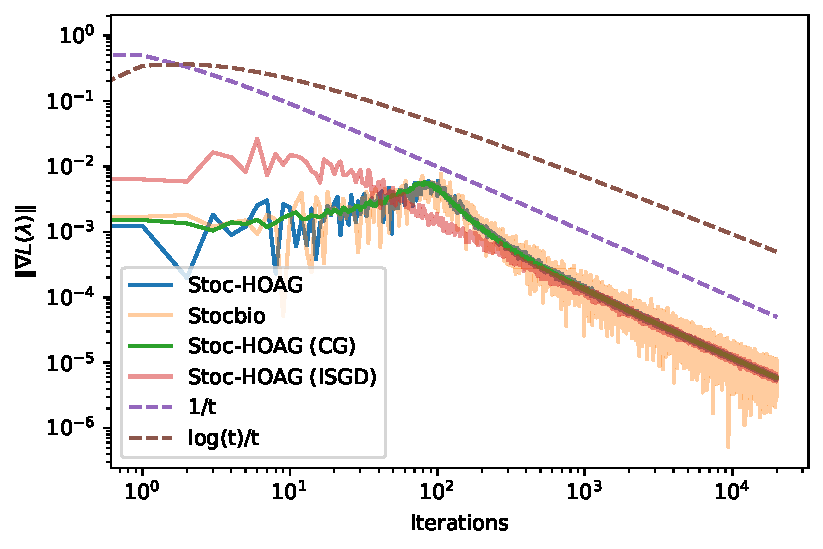
\includegraphics[width=0.5\linewidth]{IMG/stochoag/a_run_of_STHOAG_grad.pdf}
    \caption{Convergence comparison of Stocbio and Stoc-HOAG}
    \label{fig:stoc_bio_hoag}
\end{figure}

The code for reproducing numerics in this section is available at the \href{https://github.com/icheltso/thesis/tree/main/thesis\_stoc\_hoag}{thesis\_stoc\_hoag} folder of the Github repository.

\section{Conclusion}
The stocBio algorithm is one of the more recent approaches to stochastic bilevel optimisation. However, as with many other algorithms, designed to tackle bilevel problems, it suffers from a high sensitivity to the strong-convexity parameter $\mu$ of the inner level problem. In this chapter we introduce a reparametrisation for the algorithm that make it more robust in this regard, providing comparable practical convergence and improving complexity with regards to $\mu$.

%\end{thebibliography}
\addcontentsline{toc}{chapter}{References}
\bibliographystyle{plain}
\bibliography{references}

%\appendix 

\appendix
%\addcontentsline{toc}{section}{Appendix A: HOAG Proofs}
%\section*{Appendix A: HOAG Proofs}
%\label{AppendixA}
\chapter{Background Chapter Proofs}
\section{HOAG}
\begin{proof}[Proof of Theorem \ref{hoag_thm_simplified}]
An equivalent condition to $L(\lambda)$ having Lipschitz continuous gradient is that for any $\alpha,\beta \in \mathcal{D}$ \cite{Zhou2018}:
\begin{equation} \label{lipschitz_equiv}
    L(\beta) \leq L(\alpha) + \nabla L(\alpha)^\top (\beta - \alpha) + \frac{L}{2}\|\beta - \alpha\|^2.
\end{equation}
Substituting for $\alpha = \lambda_k, \beta = \lambda_{k+1} = \lambda_k - \frac{1}{L}p_k$, we add and subtract $p_k^\top(\lambda_k - \lambda_{k-1})$ to get
\begin{align}
    L(\lambda_{k+1}) &\leq L(\lambda_k) - (\nabla L(\lambda_k) -p_k)^\top(\lambda_k - \lambda_{k+1}) -p_k^\top(\lambda_k - \lambda_{k+1})+\frac{L}{2}\|\lambda_k - \lambda_{k+1}\|^2 \\
    &= L(\lambda_k) - (\nabla L(\lambda_k) -p_k)^\top(\lambda_k - \lambda_{k+1}) -\frac{1}{L}\|p_k\|^2+\frac{1}{2L}\|p_k\|^2 \quad  \label{lamline} \\
    &=L(\lambda_k) - (\nabla L(\lambda_k) -p_k)^\top(\lambda_k - \lambda_{k+1}) -\frac{1}{2L}\|p_k\|^2,
\end{align}
where in line \ref{lamline}, we use the fact, that $\lambda_{k}-\lambda_{k+1} = \frac{1}{L}p_k$. Finally, by Cauchy-Schwarz, we have
\begin{equation} \label{lip_cauchy}
    L(\lambda_{k+1}) \leq L(\lambda_k) + \|\nabla L(\lambda_k) -p_k\|\|\lambda_k - \lambda_{k+1}\| -\frac{1}{2L}\|p_k\|^2.
\end{equation}
Now, by Theorem \ref{thm_appgrad_hoag}, $\|\nabla L(\lambda_k) -p_k\| = \mathcal{O}(\epsilon_k)$. As $\mathcal{D}$ is compact, it is bounded (by Heine-Borel). So there exists some radius $R$, such that $\|\lambda\| \leq R$ for all $\lambda \in \mathcal{D}$. Thus, we have that there exists an $M>0$, such that
\[\|\nabla L(\lambda_k) -p_k\|\|\lambda_k - \lambda_{k+1}\| < 2R(C \epsilon_k) = M\epsilon_k.\]
Applying this to (\ref{lip_cauchy}), we get
\begin{equation} \label{lip_cauchy_2}
    L(\lambda_{k+1}) \leq L(\lambda_k) + M\epsilon_k -\frac{1}{2L}\|p_k\|^2.
\end{equation}
Rewriting, we get
\begin{equation} \label{lam_bound}
    \frac{1}{2L}\|p_k\|^2 \leq L(\lambda_k) - L(\lambda_{k+1}) + M\epsilon_k.
\end{equation}
By the extreme-value theorem, since $L$ is defined on a compact set and has continuous derivatives, it has a lower bound $K$. Thus, taking the sum of (\ref{lam_bound}) for $k = m$ to $\infty$, we get
\begin{equation} \label{lam_bound_sum}
   \frac{1}{2L}\sum_{k=m}^\infty \|p_k\|^2 \leq L(\lambda_m) - K + M\sum_{k=m}^\infty \epsilon_k.
\end{equation}
$\{\epsilon_k\}_{k=1}^\infty$ is summable by assumption, thus $\sum_{k=m}^\infty \epsilon_k < \infty$, $\epsilon_k \xrightarrow[]{} 0$ and the RHS of (\ref{lam_bound_sum}) is finite. Hence the LHS of (\ref{lam_bound_sum}) must also be finite. Hence $\|p_k\|^2 \xrightarrow[]{} 0 \iff \|p_k\| \xrightarrow[]{} 0.$ Recall, that $\|\nabla L(\lambda_k) - p_k\| = \mathcal{O}(\epsilon_k)$, hence 
\[\|\nabla L(\lambda_k)\| \leq \|p_k\| + \mathcal{O}(\epsilon_k) \xrightarrow[]{k \xrightarrow[]{} \infty} 0.\]
\begin{comment}
    Hence, taking limits and using the previous theorem, we get
\begin{align*}
    0 &= \lim_{k \xrightarrow[]{} \infty} \{\lambda_{k+1} - \lambda_k\} \\
      &= \lim_{k \xrightarrow[]{} \infty} \{P_\mathcal{D}(\lambda_k - \frac{1}{L}p_k) - \lambda_k\} \\
      &= P_\mathcal{D}(\lambda^* - \frac{1}{L}\nabla L(\lambda^*)) - \lambda^*.
\end{align*}
We thus obtain the fixed-point equation
\begin{equation} \label{lam_fpe}
    \lambda^* = P_\mathcal{D}(\lambda^* - \frac{1}{L}\nabla L(\lambda^*)).
\end{equation}
If we define the indicator function $I_\mathcal{D}:\mathbb{R}^r \xrightarrow[]{} \{0,\infty\}$ as
\[I_\mathcal{D}(\lambda) = 
    \begin{cases} 
      0 & \lambda \in \mathcal{D} \\
      \infty & \mathrm{otherwise},
    \end{cases}\]
then the projection operator $P_\mathcal{D}$ can be redefined as an unconstrained optimization problem:
\[P_\mathcal{D} (\alpha) = \argmin_{\lambda \in \mathbb{R}^r} I_\mathcal{D}(\lambda) + \frac{1}{2}\|\alpha - \lambda\|^2.\]
We can then use the first-order optimality condition with (\ref{lam_fpe}). We obtain, for $\alpha = \lambda^* - \frac{1}{L}\nabla L(\lambda^*)$ and $\lambda = \lambda^*$:
\begin{align}
    0 &\in \partial_\lambda \left(I_\mathcal{D}(\lambda) + \frac{1}{2}\|\alpha - \lambda\|^2 \right) \\
    0 &\in \partial_\lambda I_\mathcal{D}(\lambda) - \frac{1}{L}\nabla L(\lambda^*) \implies \\
    &\frac{1}{L}\nabla L(\lambda^*) \in \partial_\lambda I_\mathcal{D}(\lambda). \label{sugrad_ind}
\end{align}
Since $\mathcal{D}$ is convex, so is the function $I_\mathcal{D}$. By Rockafellar \& Wets \cite{var_analysis}, the subgradient of a convex function is a monotone mapping. That is, for $\lambda'_0, \lambda'_1 \in \mathcal{D}$, for all $v_0 \in \partial I_\mathcal{D}(\lambda'_0), v_1 \in \partial I_\mathcal{D}(\lambda'_1)$, we have
\[(v_1-v_0)^\top(\lambda'_1 - \lambda'_0) \geq 0.\]
Now, in terms of \cite{var_analysis}, for $\lambda'_1 \in \mathcal{D}$, either $\partial I_\mathcal{D}(\lambda'_1) = 0$ for $\lambda'_1 \in \mathrm{int}\mathcal{D}$ or $\partial I_\mathcal{D}(\lambda'_1) = [0,\infty]$ for $\lambda'_1 \in \partial\mathcal{D}$. In any case, we have that $0 \in \partial I_\mathcal{D}(\lambda'_1).$ If we let $\lambda'_1 = \lambda^*$, we have from \ref{sugrad_ind}, that
\begin{equation} \label{mon_map_grad}
    \nabla L(\lambda^*)^T(\lambda^* - \alpha) \geq 0.
\end{equation}
If $\lambda^* \in \mathrm{int} \mathcal{D}$, then fr some $t>0$, $\lambda^* \in B(\lambda^*,t) \subset \mathcal{D}.$ However, (\ref{mon_map_grad}) must be satisfied for all vectors $(\lambda^* - \alpha)$ in $B(\lambda^*,t)$. As $B(\lambda^*,t)$ contains a basis for $\mathbb{R}^r$, necessarily, 
\[\nabla L(\lambda^*) = 0.\]
\end{comment}

\end{proof}


\chapter{Chapter III Proofs}
\label{Bayesian_proofs}
\begin{comment}
    \begin{proof}[Change of variable for Theorem \ref{thm:overparam}]
We begin by expanding the left-hand side
    \begin{align*}
    \int_X \phi(u \odot v) \,\pi(u,v)\,\mathrm{d}u\,dv &= \frac{1}{Z_\pi}  \int_{\mathbb{R}^d} \int_{(0,\infty)^d} \phi(u \odot v) \\
    &\quad\times\prod_{i=1}^d u_{i} \exp{ \left(-\beta \left(\lambda (\|u\|_2^2 + \|v\|_2^2)/2 + G(u \odot v) \right) \right)}\, \mathrm{d}u \,\mathrm{d}v.
    \end{align*}
    Consider the change of variables $x = u \odot v$ and $t = u \odot u/2$. Then $v \odot v = \frac{x \odot x}{2t}$ and $J = (\partial(z,t) / \partial(u,v))$ is a $2d \times 2d$ block-matrix, where
    $$\operatorname{det}J 
    = 
    \operatorname{det}\begin{pmatrix}
     \nabla_u x(u,v) && \nabla_v x(u,v) \\
     \nabla_u t(u,v) && \nabla_v t(u,v)
    \end{pmatrix} =\operatorname{det}\begin{pmatrix}
     \diag(v) && \diag(u) \\
     \diag(u) && 0
    \end{pmatrix} = \prod_{i=1}^d u_i^2.$$ 
    Thus, $\mathrm{d}u\,\mathrm{d}v = \frac{1}{|\mathrm{det}J|} \mathrm{d}
    x\,\mathrm{d}t = \frac{1}{\prod_{i=1}^d u_i^2} \mathrm{d}x\,\mathrm{d}t$ and so, 
    \begin{align*}   
    &\int \phi(u\odot v)\, \pi(u,v)\,\mathrm{d}u\,dv \\
       & = \frac{1}{(\sqrt{2})^d Z_\pi} \int_{\mathbb{R}^d} \phi(x) \exp{\left( -\beta G(x) \right)} \prod_{i=1}^d \left( \int_{0}^\infty t_i^{-\frac{1}{2}}\exp{ \left(-\beta \lambda \left(t_i + \frac{x_i^2}{4t_i} \right) \right)} \mathrm{d}t_i \right) \mathrm{d}x\\
       &= \frac{1}{Z_\pi} \left(\sqrt{\frac{\pi}{2\beta \lambda}}\right)^d \int_{\real^d} \phi(x) \exp{\left(-\beta \left(\lambda \|x\|_1 + G(x) \right) \right)}\mathrm{d}x
    \end{align*}
    where the last line follows from \eqref{eq:laplace}.
\end{proof}
\end{comment}


\begin{proof}[Change of variable for Theorem \ref{thm:overparam}]
We apply a change of variables of $x = u \odot v$ and $\eta = u \odot u /(\lambda \beta)$ to \eqref{eq:gibbs}. 
Indeed, we then have $x_i^2/\eta = \lambda\beta v_i^2$ and so $J = (\partial(x,\eta) / \partial(u,v))$ is a $2d \times 2d$ block-matrix, where
    $$\operatorname{det}J 
    = 
    \operatorname{det}\begin{pmatrix}
     \nabla_u x(u,v) && \nabla_v x(u,v) \\
     \nabla_u \eta(u,v) && \nabla_v \eta(u,v)
    \end{pmatrix} =\operatorname{det}\begin{pmatrix}
     \diag(v) && \diag(u) \\
     \diag(2u/\lambda\beta) && 0
    \end{pmatrix} = \prod_{i=1}^d 2u_i^2/\lambda\beta.$$
Thus, $\mathrm{d}u\,\mathrm{d}v = \frac{1}{|\mathrm{det}J|} \mathrm{d}
    x\,\mathrm{d}\eta = \frac{\lambda\beta}{\prod_{i=1}^d 2u_i^2} \mathrm{d}x\,\mathrm{d}\eta$, and so
\begin{align*}
    &\int \phi(x)\rho(x)\, dx = \int \int \phi(x) \tilde \pi(x,\eta)\,d\eta \,dx\\
    &=\int \int \phi(x) \frac{1}{\prod_{i} \sqrt{\eta_i}} \exp\pa{  -\sum_i \pa{ \frac{x_i^2}{2\eta_i} + \frac{\beta^2\lambda^2\eta_i}{2} -\beta G(x)} } \,dx\,d\eta\\
    &=\int \int \phi(u\odot v) \frac{1}{\prod_{i} u_i/(\sqrt{\lambda \beta})} \exp\pa{  -\frac{\beta\lambda}{2}\sum_i \pa{ v_i^2+u_i^2 } -\beta G(u\odot v) } \prod_i (2u_i^2/\lambda \beta) \,du\, dv\\
    &= 2^d (\lambda\beta)^{-d/2} \int \int \phi(u\odot v)  \exp\pa{  -\frac{\beta\lambda}{2}\sum_i \pa{  v_i^2+u_i^2 } -\beta G(u\odot v) } \prod_i u_i \,du\, dv.
\end{align*}
\end{proof}

\chapter{Chapter IV Proofs}
\label{bilevel_proofs}

\section{Stocbio/Stoc-HOAG}
\subsection*{Appendix A: Helpful Results}
\label{AppendixA}
We begin by providing a few error bounds for SGD. Firstly, we can directly obtain the iterate error for the strongly convex case as follows.
\begin{lemma}[Iterate error: SGD for $\mu-$st. conv.] \label{sgdmu}
    Suppose $F$ is $\mu-$strongly convex over a convex set $\chi$. Assume the stochastic gradient at step $t$, $\tilde{\nabla} F_t$ is such that $\mathbb{E}[\tilde{\nabla} F_t] = \nabla F(x_t)$ and $ \mathbb{E}[\|\tilde{\nabla} F_t\|^2] \leq G^2.$ Then, if we choose the stepsize $\eta_t = \frac{1}{\mu t}$, we have the following error bound:
    \[\mathbb{E}[\|x_T - x^*\|^2] \leq \frac{4G^2}{\mu^2 T}.\]
\end{lemma}
\begin{proof}
    Using strong convexity, we have
        \begin{equation} \label{must}
            \nabla F(x_t)^T(x_t - x^*) \geq F(x_t) - F(x^*) + \frac{\mu}{2}\|x_t - x^*\|^2.
        \end{equation}
        Furthermore, since $x^*$ is a minimizer, we have that $\nabla F(x^*)^T(x_t - x^*) = 0$ and so
        \begin{equation} \label{must_opt}
            F(x_t) - F(x^*) \geq \frac{\mu}{2}\|x_t - x^*\|^2.
        \end{equation}
        Using (\ref{must}) and (\ref{must_opt}), we obtain
        \[\mathbb{E}[\|x_{t+1} - x^*\|^2] = \mathbb{E}[\|x_t - \eta_t \tilde{\nabla} F_t - x^*\|^2] =\]
        \[=\mathbb{E}[\|x_{t} - x^*\|^2] - 2\eta_t \mathbb{E} \left[ \tilde{\nabla} F_t^T(x_t - x^*) \right] + \eta^2 \mathbb{E}[\|\tilde{\nabla} F_t\|^2] \]
        \[\leq \mathbb{E}[\|x_{t} - x^*\|^2] - 2\eta_t \mathbb{E} \left[F(x_t) - F(x^*) + \frac{\mu}{2}\|x_t - x^*\|^2 \right] + \eta^2 \mathbb{E}[\|\tilde{\nabla} F_t\|^2]\]
        \[\leq \mathbb{E}[\|x_{t} - x^*\|^2] - 2\eta_t \mathbb{E} \left[\frac{\mu}{2}\|x_t - x^*\|^2 + \frac{\mu}{2}\|x_t - x^*\|^2 \right] + \eta^2 \mathbb{E}[\|\tilde{\nabla} F_t\|^2] \]
        \begin{equation} \label{2eta}
            = (1-2\eta_t \mu) \mathbb{E}\|x_t - x^*\|^2 + \eta_t^2 G^2.
        \end{equation}
        Note, that for $t=1$, $\mu-$strong convexity and Cauchy-Schwarz give us
        \[(\nabla F(x_1) - \nabla F(x^*))^T(x_1-x^*) \geq \frac{\mu}{2}\|x_1 - x^*\|\]
        \[\implies \|\nabla F(x_1)\|^2 \geq \frac{\mu^2}{4}\|x_1 - x^*\|^2.\]
        Finally, by the fact, that $\mathbb{E}\|\tilde{\nabla}F_1\|^2 \geq \mathbb{E}\|\tilde{\nabla}F(x_1)\|^2$, we get
        \[\mathbb{E}\|x_1 - x^*\|^2 \leq \frac{4}{\mu^2} \mathbb{E}\|\tilde{\nabla}F_1\|^2 \leq \frac{4G^2}{\mu^2}\]
        Using the stepsize $\eta_t = \frac{1}{\mu t}$ in (\ref{2eta}), we get the inequality
        \[\mathbb{E}[\|x_{t+1} - x^*\|^2] \leq (1-2/t) \mathbb{E}\|x_t - x^*\|^2 + \eta_t^2 G^2.\]
        The cases $t=1,2,3$ are easily confirmed. To finish the proof we do induction with base case $t=3$.
\end{proof}

\subsection*{Appendix B: Proofs for Neumann Series and $\widehat{\nabla} \mathcal{L}$} \label{AppendixB}
\begin{proof}[Proof of proposition \ref{evq_bnd}]
\begin{comment}
    \[\mathbb{E}v_Q = \|\eta \sum_{i=0}^Q(I - \eta \nabla_{xx}^2 F)^i \nabla_x C\| \leq \eta \|\sum_{i=0}^Q(I - \eta \nabla_{xx}^2 F)^i\| \|\nabla_x C\| \leq \eta M \sum_{i=0}^Q(1 - \eta\mu)^i = \eta M \frac{1 - (1-\eta\mu)^{Q+1}}{\eta\mu}\]
\[= \frac{M}{\mu}\left(1 - (1-\eta\mu)^{Q+1} \right).\]
\end{comment}
\begin{align}
\mathbb{E}v_Q 
&= \left\| \eta \sum_{i=0}^Q (I - \eta \nabla_{xx}^2 F)^i \nabla_x C \right\| \leq \eta \left\| \sum_{i=0}^Q (I - \eta \nabla_{xx}^2 F)^i \right\| \cdot \|\nabla_x C\| \notag \\
&\leq \eta M \sum_{i=0}^Q (1 - \eta\mu)^i = \eta M \frac{1 - (1 - \eta\mu)^{Q+1}}{\eta\mu} \notag = \frac{M}{\mu} \left( 1 - (1 - \eta\mu)^{Q+1} \right),
\end{align}
where, in the second line, we used the fact that, due to strong convexity, the eigenvalues of the hessian $\nabla_{xx}^2 F$ are at least $\mu$.
\end{proof}

\begin{proof}[Proof of Proposition \ref{varvq_better}.]
Denote
\begin{align*}
    A_j &= I- \eta \nabla_{xx}^2 \tilde{F}(x_k,\lambda_k, \mathcal{B}_j); \\
    \tilde{B} &= \nabla_x \tilde{C} (x_k,\lambda_k,\zeta); \\
    A &= \mathbb{E}A_j = I- \eta \nabla_{xx}^2 F(x_k,\lambda_k); \\
    B &= \mathbb{E}B = \nabla_x C (x_k,\lambda_k);
\end{align*}
Then 
\[\mathrm{Var}(v_Q) = \mathbb{E} \|v_Q - \mathbb{E}v_Q \|^2\]

\[= \mathbb{E} \left\|\eta \sum_{q=-1}^{Q-1} \prod_{j = Q-q}^Q A_j \tilde{B} - \eta \sum_{i=0}^Q A^i B \right\|^2\]

\[\leq 2 \mathbb{E} \left\| \eta \sum_{q=-1}^{Q-1} \prod_{j = Q-q}^Q A_j \tilde{B} - \eta \sum_{i=0}^Q A^i \tilde{B} \right\|^2 + 2\mathbb{E} \left\| \eta \sum_{i=0}^Q A^i \tilde{B} - \eta \sum_{i=0}^Q A^i B \right\|^2 \]

\[= 2 \mathbb{E} \left\| \eta \sum_{q=-1}^{Q-1} \left( \prod_{j = Q-q}^Q A_j - A^{q+1} \right) \tilde{B} \right\|^2 + 2\mathbb{E} \left\| \eta \sum_{i=0}^Q A^i (\tilde{B} - B) \right\|^2. \]
Now, note that $\mathbb{E}\left( \prod_{j = Q-q}^Q A_j - A^{q+1} \right) = 0$, since each $A_i$ is independently sampled. Due to this, when expanding the square of the first sum above, the cross terms vanish in expectation, and so
{\setlength{\abovedisplayskip}{6pt}
 \setlength{\belowdisplayskip}{6pt}
\begin{align*}
& 2 \mathbb{E} \left\| \eta \sum_{q=-1}^{Q-1} 
   \left( \prod_{j = Q-q}^Q A_j - A^{q+1} \right) \tilde{B} \right\|^2 + 2\mathbb{E} \left\| \eta \sum_{i=0}^Q A^i (\tilde{B} - B) \right\|^2 \\
&\leq 2 \eta^2 \sum_{q=-1}^{Q-1} 
   \mathbb{E} \left\| \prod_{j = Q-q}^Q A_j - A^{q+1} \right\|^2 
   \mathbb{E} \left\| \tilde{B} \right\|^2 + 2\eta^2 \sum_{i=0}^Q \|  A \|^{2i} \mathbb{E} \|\tilde{B} - B\|^2 \\
&= 2 \eta^2 \sum_{q=0}^{Q} 
   \mathbb{E} \left\| \prod_{j = Q-q+1}^Q A_j - A^{q} \right\|^2 
   \mathbb{E} \left\| \tilde{B} \right\|^2 + 2\eta^2 \frac{1-\|A\|^{2Q}}{1-\|A\|^2} 
   \mathbb{E} \|\tilde{B} - B\|^2.
\end{align*}}
%\[2 \mathbb{E} \left\| \eta \sum_{q=-1}^{Q-1} \left( \prod_{j = Q-q}^Q A_j - A^{q+1} \right) \tilde{B} \right\|^2 + 2\mathbb{E} \left\| \eta \sum_{i=0}^Q A^i (\tilde{B} - B) \right\|^2 \]

%\[\leq 2 \eta^2 \sum_{q=-1}^{Q-1} \mathbb{E} \left\| \left( \prod_{j = Q-q}^Q A_j - A^{q+1} \right) \tilde{B} \right\|^2 + 2\eta^2 \left\| \sum_{i=0}^Q  A^i \right\|^{2} \mathbb{E} \|\tilde{B} - B\|^2 \]

%\[\leq 2 \eta^2 \sum_{q=-1}^{Q-1} \mathbb{E} \left\| \prod_{j = Q-q}^Q A_j - A^{q+1} \right \|^2 \mathbb{E} \left\| \tilde{B} \right\|^2 + 2\eta^2 \sum_{i=0}^Q \|  A \|^{2i} \mathbb{E} \|\tilde{B} - B\|^2 \]

%\[= 2 \eta^2 \sum_{q=0}^{Q} \mathbb{E} \left\| \prod_{j = Q-q+1}^Q A_j - A^{q} \right \|^2 \mathbb{E} \left\| \tilde{B} \right\|^2 + 2\eta^2 \frac{1-\|A\|^{2Q}}{1-\|A\|^2} \mathbb{E} \|\tilde{B} - B\|^2\]
We will now bound $\mathbb{E}M_i$ for $M_i = \left\| \prod_{j = Q-i+1}^Q A_j - A^{i} \right \|^2$. Note, that $M_0 = 0.$ As in the proof of Proposition 3 in \cite{ji2021bilevel}, we write
 \[\prod_{j=Q-q + 1}^Q\left(I- \eta \nabla_{xx}^2 \tilde{F}_j\right) = \prod_{j=Q-q + 2}^Q \left(I- \eta \nabla_{xx}^2 \tilde{F}_j\right) - \eta \nabla_x^2 \tilde{F}_j\prod_{j=Q-q + 2}^Q\left(I- \eta \nabla_{xx}^2 \tilde{F}_j\right) \]
Then, we have (denoting $\tilde{F}\left(x_k, \lambda_k ; \mathcal{B}_j\right) = \tilde{F}_j$)
\[\mathbb{E} M_i = \mathbb{E} \left\| \prod_{j=Q-i+1}^Q\left(I- \eta \nabla_{xx}^2 \tilde{F}\left(x_k, \lambda_k ; \mathcal{B}_j\right)\right) -  \left[I - \eta\nabla_{xx}^2 F \left(x_k, \lambda_k\right)\right]^i \right\|^2\]
\[ = \mathbb{E} \left\| \prod_{j=Q-i + 2}^Q \left(I- \eta \nabla_{xx}^2 \tilde{F}_j\right) - \eta \nabla_x^2 \tilde{F}_{Q-i+1}\prod_{j=Q-i + 2}^Q\left(I- \eta \nabla_{xx}^2 \tilde{F}_j\right) - \left[I - \eta\nabla_{xx}^2 F \left(x_k, \lambda_k\right)\right]^i \right\|^2\]
Add and subtract $\eta \nabla_x^2 F \prod_{j = Q + 2 - i}(I - \eta \nabla_x^2 \tilde{F}_j)$:
\begin{align}
    \mathbb{E} \Bigg\| 
    &\left( \underbrace{(I - \eta \nabla_x^2 F) 
    \prod_{j=Q - i + 2}^Q \left(I - \eta \nabla_{xx}^2 \tilde{F}_j\right) 
    - \left[I - \eta \nabla_{xx}^2 F(x_k, \lambda_k)\right]^i}_{c} \right) \notag \\
    &+ \left( \underbrace{
    (\eta \nabla_x^2 F - \eta \nabla_x^2 \tilde{F}_{Q - i + 1}) 
    \prod_{j=Q - i + 2}^Q \left(I - \eta \nabla_{xx}^2 \tilde{F}_j\right)
    }_{d} \right)
    \Bigg\|^2 \\
    &=\mathbb{E}\|c\|^2 + \mathbb{E}\|d\|^2 + \underbrace{2\mathbb{E}\langle c,d \rangle}_{=0 \text{ as } \mathbb{E}(\eta \nabla_x^2 F - \eta \nabla_x^2 \tilde{F}_j) = 0}
\end{align}
    Note, that for sample set $\mathcal{B}_{Q-i+1} = \{\xi_j, j=1,\hdots,|\mathcal{B}_{Q-i+1} |\}$, with i.i.d. $\xi_j$, by Proposition \ref{boun_var}, we obtain
    \[\mathbb{E}\|\nabla_x^2 F(x_k,\lambda_k) - \nabla_x^2 \tilde{F}_{Q-i+1}\|^2 = \mathbb{E} \left\|\frac{1}{|\mathcal{B}_{Q-i+1}|} \sum_{j=1}^{|\mathcal{B}_{Q-i+1}|} \left(\nabla_x^2 F(x_k,\lambda_k) - \nabla_x^2 \tilde{F}(x_k,\lambda_k,\xi_j) \right) \right\|^2\]
    \begin{equation} \label{var_samp_bound}
        =\frac{1}{|\mathcal{B}_{Q-i+1}|^2}\sum_{j=1}^{|\mathcal{B}_{Q-i+1}|}\mathbb{E}_{\xi_j} \|\nabla_x^2 F(x_k,\lambda_k) - \nabla_x^2 \tilde{F}(x_k,\lambda_k,\xi_j)\|^2 \leq \frac{L^2}{|\mathcal{B}_{Q-i+1}|}
    \end{equation}
    Hence, by strong convexity and Cauchy-Schwarz we obtain that
    \[\mathbb{E}\|c\|^2 \leq (1-\eta \mu)^2 \mathbb{E} M_{i-1}, \quad \mathbb{E}\|d\|^2 \leq  \eta^2 (1-\eta \mu)^{2i-2} \frac{L^2}{|\mathcal{B}_{Q-i+1}|}.\]
    That is, 
    \[\mathbb{E}M_i \leq (1-\eta \mu)^2 \mathbb{E} M_{i-1} + \eta^2 (1-\eta \mu)^{2i-2} \frac{L^2}{|\mathcal{B}_{Q-i+1}|}.\]
    Telescoping, we get
    \[\mathbb{E}M_i \leq (1-\eta \mu)^{2k} \mathbb{E}M_{i-k} + \eta^2L^2(1-\eta\mu)^{2i-2} \sum_{j=1}^{k} \frac{1}{|\mathcal{B}_{Q-i+j}|} \]
    Setting $i=q, k = q,$
    %\[\mathbb{E}M_q \leq (1-\eta \mu)^{2q} \mathbb{E}M_{0} + \eta^2L^2 (1-\eta\mu)^{2q-2} \sum_{j=0}^{q-1} \frac{(1-\eta\mu)^{2j}}{|\mathcal{B}_{Q-(q-j)+1}|}\]
    \[\mathbb{E}M_q \leq (1-\eta \mu)^{2q} \mathbb{E}M_{0} + \eta^2L^2 (1-\eta\mu)^{2q-2} \sum_{j=1}^{q} \frac{1}{|\mathcal{B}_{Q-1+j}|}\]
    Note that $\mathbb{E}(M_0) = 0$.
    %by Lemma 1 of \cite{stocBio}
    %\[\mathbb{E}M_1 = \mathbb{E}\|(I - \eta\nabla_x^2 \tilde{F}_Q) - (I - \eta \nabla_x^2 F)\|^2 = \eta^2 \mathbb{E} \|\nabla_x^2 F - \nabla_x^2 \tilde{F}_Q\|^2 \leq \eta^2 L^2\]
    Now, setting $|\mathcal{B}_{Q-1+j}| = B(1-\eta\mu)^{j-1}$, we finally get
    \[
        \mathbb{E}M_q \leq \eta^2L^2 (1-\eta\mu)^{2q-2} \sum_{j=1}^{q} \frac{1}{B(1-\eta\mu)^{j-1}} = \frac{\eta^2L^2 (1-\eta\mu)^{2q-2}}{B}  \frac{\left(\frac{1}{1-\eta \mu}\right)^{q}-1}{\frac{1}{1-\eta \mu}-1}
    \]
    \begin{equation} \label{EM_bound2}
        \leq \frac{\eta L^2 (1-\eta\mu)^{q}}{B(1-\eta\mu)\mu}.
    \end{equation}

%Hence,
%\[\mathbb{E} \left\| \prod_{j = Q-q+1}^Q A_j - A^{q} \right \|^2 \leq \eta^2 L^2 (1-\eta\mu)^{2q-2} \frac{1-(1-\eta \mu)^{q+1}}{1-(1-\eta \mu)} = \frac{\eta L^2}{\mu} \left((1-\eta \mu)^{2q-2} - (1-\eta \mu)^{3q-1}\right)\]
In a fashion similar to (\ref{var_samp_bound}), we obtain $\mathbb{E} \|\tilde{B} - B\|^2 \leq \frac{M^2}{|\mathcal{S}_{\nabla_x C,k}|}$. Hence, using the continuity and convexity assumptions, we get

\[\mathrm{Var}(v_Q) \leq 2 \eta^2 \sum_{q=0}^{Q} \mathbb{E} M_q \mathbb{E} \left\| \tilde{B} \right\|^2 + 2\eta^2 \frac{1-\|A\|^{2Q}}{1-\|A\|^2} \mathbb{E} \|\tilde{B} - B\|^2\]

\[\leq 2 \eta^2M^2 \left( \sum_{q=0}^{Q} \frac{\eta L^2 (1-\eta\mu)^{q}}{B(1-\eta\mu)\mu} + \frac{1}{|\mathcal{S}_{\nabla_x C,k}|}\frac{1-(1-\eta\mu)^{2Q}}{1-(1-\eta\mu)^2} \right).\]

Using the fact, that $\sum_{q=0}^N x^q \leq \frac{1}{1-x}$, we get

\[ \mathrm{Var}(v_Q) \leq  2 \eta^2M^2 \left( \frac{ L^2 }{B(1-\eta\mu)\mu^2} + \frac{1}{|\mathcal{S}_{\nabla_x C,k}|}\frac{1-(1-\eta\mu)^{2Q}}{1-(1-\eta\mu)^2} \right)\]


Finally, taking into account, that $\kappa = \frac{L}{\mu}$, we get
\[\mathrm{Var}(v_Q) \leq 2 \eta^2M^2 \left( \frac{ \kappa^2 }{B(1-\eta\mu)} + \frac{1}{|\mathcal{S}_{\nabla_x C,k}|}\frac{1}{2\eta \mu - \eta^2 \mu^2} \right).\]
In the case, that $v_0 = \nabla_x C(x_k,\lambda_k)$, we have
\[\mathbb{E}\|v_Q - E(v_Q)\|^2 = \mathbb{E} \left\|\eta \sum_{q=-1}^{Q-1} \prod_{j = Q-q}^Q A_jB - \eta \sum_{i=0}^Q A^i B \right\|^2 \leq \mathbb{E} \left\|\eta \sum_{q=-1}^{Q-1} \left( \prod_{j = Q-q}^Q A_j - A^{q+1} \right) \right\|^2 \|B\|^2;\]
Proceeding as before, we obtain
\[\mathbb{E}\|v_Q - E(v_Q)\|^2 \leq \frac{\eta^2M^2 \kappa^2 }{B(1-\eta\mu)}.\]
\end{proof}



\begin{comment}

\begin{proof}[Proof of Proposition \ref{bound_nabla_hat}.]
    \[\mathrm{Var}(\widehat{\nabla}\mathcal{L}(\lambda_k)) =  \mathbb{E}\|\widehat{\nabla}\mathcal{L}(\lambda_k) - \mathbb{E}\widehat{\nabla}\mathcal{L}(\lambda_k)\|^2 = \]
\[\mathbb{E}\| \nabla_\lambda \tilde{C}(x_k,\lambda_k,\xi_1) - \nabla_{x \lambda}^2 \tilde{F}(x_k,\lambda_k,\xi_2)^\top v_Q - \left(\nabla_\lambda C (x_k,\lambda_k) - \nabla_{x \lambda}^2 F (x_k,\lambda_k)^\top \mathbb{E} v_Q \right)\|^2\]

%Expanding this, we get
\[= \mathbb{E}\|\nabla_\lambda \tilde{C}(x_k,\lambda_k,\xi_1) - \nabla_\lambda C (x_k,\lambda_k)\|^2 + \mathbb{E}\|\nabla_{x \lambda}^2 F (x_k,\lambda_k)^\top \mathbb{E} v_Q - \nabla_{x \lambda}^2 \tilde{F}(x_k,\lambda_k,\xi_2)^\top v_Q\|^2 - \]
\[- 2\mathbb{E}\left[\left(\underbrace{\nabla_\lambda \tilde{C}(x_k,\lambda_k,\xi_1) - \nabla_\lambda C (x_k,\lambda_k)}_{\mathbf{0} \text{ in expectation}}\right)^\top \left(\nabla_{x \lambda}^2 F (x_k,\lambda_k)^\top \mathbb{E} v_Q - \nabla_{x \lambda}^2 \tilde{F}(x_k,\lambda_k,\xi_2)^\top v_Q\right) \right]\]

\[= \mathbb{E}\|\nabla_\lambda \tilde{C}(x_k,\lambda_k,\xi_1) - \nabla_\lambda C (x_k,\lambda_k)\|^2 + \mathbb{E}\|\nabla_{x \lambda}^2 F (x_k,\lambda_k)^\top \mathbb{E} v_Q - \nabla_{x \lambda}^2 \tilde{F}(x_k,\lambda_k,\xi_2)^\top v_Q\|^2\]

\begin{equation} \label{ind_var_nabhatprop}
    =\mathrm{Var}\left(\nabla_\lambda \tilde{C}(x_k,\lambda_k,\xi_1) \right) + \mathrm{Var}\left(\nabla_{x \lambda}^2 \tilde{F}(x_k,\lambda_k,\xi_2)^\top v_Q \right)
\end{equation}

\[=\mathrm{Var}\left(\nabla_\lambda \tilde{C}(x_k,\lambda_k,\xi_1) \right) + \mathrm{Var}\left(\nabla_{x \lambda}^2 \tilde{F}(x_k,\lambda_k,\xi_2) \right) \mathrm{Var} \left(v_Q \right) + \mathrm{Var}\left(\nabla_{x \lambda}^2 \tilde{F}(x_k,\lambda_k,\xi_2) \right) \|\mathbb{E}[v_Q]\|^2 +  \]

\begin{equation} \label{varvq_unbound}
    + \mathrm{Var}\left(v_Q \right) \left\|\mathbb{E}\left[\nabla_{x \lambda}^2 \tilde{F}(x_k,\lambda_k,\xi_2)\right]\right\|^2,
\end{equation}
where we get from (\ref{ind_var_nabhatprop}) to (\ref{varvq_unbound}) using the the identity $\mathrm{Var}[XY] = \mathrm{Var}[X]\mathrm{Var}[Y] + \mathrm{Var}[X] \mathbb{E}[Y]^2 + \mathrm{Var}[Y] \mathbb{E}[X]^2$ for independent $X,Y$. Now, by Proposition \ref{boun_var}, and Assumption \ref{nablaFxl_bnd}, we have 
\[\mathrm{Var}\left(\nabla_\lambda \tilde{C}(x_k,\lambda_k,\xi_1) \right) \leq \frac{M^2}{|\mathcal{S}_{\nabla_{\lambda} C,k}|}, \quad \mathrm{Var}\left(\nabla_{x \lambda}^2 \tilde{F}(x_k,\lambda_k,\xi_2) \right) \leq \frac{L^2}{|\mathcal{S}_{\nabla_{x\lambda} F,k}|},\] 
\[\left\|\mathbb{E}\left[\nabla_{x \lambda}^2 \tilde{F}(x_k,\lambda_k,\xi_2)\right]\right\|^2 \leq E^2.\]
By Proposition \ref{evq_bnd}, we also obtain
\[\|\mathbb{E}[v_Q]\|^2 \leq \frac{M^2}{\mu^2}(1-(1-\eta\mu)^{Q+1})^2 \leq \frac{M^2}{\mu^2}.\]
Finally, from Proposition \ref{varvq_better}, we have
\[\mathrm{Var}(v_Q) \leq  2\eta^2M^2\left(\frac{\kappa^2}{B (2 - \eta \mu)^2} + \frac{1}{|\mathcal{S}_{\nabla_{x} C,k}|(2\eta \mu - \eta^2 \mu^2)} \right).\]

Thus, we can bound (\ref{varvq_unbound}) by 
\[2\eta^2M^2\left(\frac{\kappa^2}{B_k (2 - \eta \mu)^2} + \frac{1}{|\mathcal{S}_{\nabla_{x} C,k}|(2\eta \mu - \eta^2 \mu^2)} \right)\left(\frac{L^2}{|\mathcal{S}_{\nabla_{x\lambda} F,k}|} + E^2\right)  +  \frac{\kappa^2M^2}{|\mathcal{S}_{\nabla_{x\lambda} F,k}|}+ \frac{M^2}{|\mathcal{S}_{\nabla_{\lambda} C,k}|},\]
and we are done.

%Add and subtract $\nabla_{x \lambda}^2 F ^\top v_Q$:
%\[\mathbb{E}\| \nabla_\lambda \tilde{C}(x_k,\lambda_k,\xi_1) - \nabla_\lambda C (x_k,\lambda_k) +(\nabla_{x \lambda}^2 F (x_k,\lambda_k) - \nabla_{x \lambda}^2 \tilde{F}(x_k,\lambda_k,\xi_2))^\top v_Q + \nabla_{x \lambda}^2 F (x_k,\lambda_k)^\top (\mathbb{E} v_Q - v_Q)\|^2\]
\end{proof}

\end{comment}

\begin{proof}[Proof of Proposition \ref{bound_nabla_hat}]
We have
\[
\mathrm{Var}(\widehat{\nabla}\mathcal{L}(\lambda_k)) 
= \mathbb{E}\big\|\widehat{\nabla}\mathcal{L}(\lambda_k) - \mathbb{E}[\widehat{\nabla}\mathcal{L}(\lambda_k)]\big\|^2,
\]
where
\[
\widehat{\nabla}\mathcal{L}(\lambda_k) 
= \nabla_\lambda \tilde{C}(x_k,\lambda_k,\xi_1) 
- \nabla_{x \lambda}^2 \tilde{F}(x_k,\lambda_k,\xi_2)^\top v_Q.
\]

Expanding and subtracting expectations, we obtain
\[
\begin{aligned}
& \nabla_\lambda \tilde{C}(x_k,\lambda_k,\xi_1) 
- \nabla_{x \lambda}^2 \tilde{F}(x_k,\lambda_k,\xi_2)^\top v_Q
- \big(\nabla_\lambda C(x_k,\lambda_k) - \nabla_{x \lambda}^2 F(x_k,\lambda_k)^\top \mathbb{E}[v_Q]\big) \\
&= (\nabla_\lambda \tilde{C}(x_k,\lambda_k,\xi_1) - \nabla_\lambda C(x_k,\lambda_k)) \\
&\quad + (\nabla_{x \lambda}^2 \tilde{F}(x_k,\lambda_k,\xi_2) - \mathbb{E}[\nabla_{x \lambda}^2 \tilde{F}(x_k,\lambda_k,\xi_2)])^\top v_Q \\
&\quad + \mathbb{E}[\nabla_{x \lambda}^2 \tilde{F}(x_k,\lambda_k,\xi_2)]^\top (v_Q - \mathbb{E}[v_Q]).
\end{aligned}
\]
Note, that the first term has zero mean in expectation. Thus, the cross-product terms die out when we expand the square
\[
\mathrm{Var}(\widehat{\nabla}\mathcal{L}(\lambda_k)) 
= \mathbb{E}\big\|\widehat{\nabla}\mathcal{L}(\lambda_k) - \mathbb{E}[\widehat{\nabla}\mathcal{L}(\lambda_k)]\big\|^2
\]
\[= \mathbb{E}\|\nabla_\lambda \tilde{C}(x_k,\lambda_k,\xi_1) - \nabla_\lambda C (x_k,\lambda_k)\|^2 + \mathbb{E}\|\nabla_{x \lambda}^2 F (x_k,\lambda_k)^\top \mathbb{E} v_Q - \nabla_{x \lambda}^2 \tilde{F}(x_k,\lambda_k,\xi_2)^\top v_Q\|^2\]

\begin{equation} \label{ind_var_nabhatprop}
    =\mathrm{Var}\left(\nabla_\lambda \tilde{C}(x_k,\lambda_k,\xi_1) \right) + \mathrm{Var}\left(\nabla_{x \lambda}^2 \tilde{F}(x_k,\lambda_k,\xi_2)^\top v_Q \right)
\end{equation}

Let 
\[
X := \nabla_{x \lambda}^2 \tilde{F}(x_k,\lambda_k,\xi_2), \quad 
\]
Then, by Lemma \ref{var_lemma_appendix}, the following inequality holds:
\[
\mathrm{Var}[X^\top v_Q]
\leq 2 \, \mathrm{Var}[X] \, \mathbb{E}\|v_Q\|^2 
+ 2 \, \|\mathbb{E}[X]\|^2 \, \mathrm{Var}[v_Q].
\]
By Assumptions and Proposition \ref{boun_var},
\[
\mathrm{Var}(\nabla_\lambda \tilde{C}) \leq \tfrac{M^2}{|\mathcal{S}_{\nabla_\lambda C,k}|}, 
\quad \mathrm{Var}[X] \leq \tfrac{L^2}{|\mathcal{S}_{\nabla_{x\lambda} F,k}|}, 
\quad \|\mathbb{E}[X]\|^2 \leq E^2.
\]
Furthermore, from Propositions \ref{evq_bnd} and \ref{varvq_better},
\[
\|\mathbb{E}[v_Q]\|^2 \leq \tfrac{M^2}{\mu^2}, 
\quad \mathrm{Var}(v_Q) \leq 2\eta^2 M^2 \left( \tfrac{\kappa^2}{B (2 - \eta \mu)^2} 
+ \tfrac{1}{|\mathcal{S}_{\nabla_x C,k}|(2\eta \mu - \eta^2 \mu^2)} \right).
\]
Hence,
\[
\mathrm{Var}(\widehat{\nabla}\mathcal{L}(\lambda_k)) 
\leq \frac{M^2}{|\mathcal{S}_{\nabla_\lambda C,k}|} 
+ 2 \frac{L^2 M^2}{\mu^2|\mathcal{S}_{\nabla_{x\lambda} F,k}|} \, 
+ 4E^2\eta^2 M^2 \left( \tfrac{\kappa^2}{B (2 - \eta \mu)^2} 
+ \tfrac{1}{|\mathcal{S}_{\nabla_x C,k}|(2\eta \mu - \eta^2 \mu^2)} \right).
\]
\end{proof}


\begin{lemma}[Variance bound for $X^\top Y$] \label{var_lemma_appendix}
\label{lem:var_XtY}
Let \(X\in\mathbb{R}^{d_x\times d_\lambda}\) and \(Y\in\mathbb{R}^{d_x}\) be random variables with finite second moments, and assume \(X\) and \(Y\) are independent. Denote
\[
Z := X^\top Y \in \mathbb{R}^{d_\lambda}.
\]
Then
\[
\mathrm{Var}[Z] \;=\; \mathbb{E}\big\|Z - \mathbb{E}[Z]\big\|^2
\;\le\; 2\,\mathrm{Var}[X] \,\mathbb{E}\|Y\|^2
\;+\; 2\,\big\|\mathbb{E}[X]\big\|^2 \,\mathrm{Var}[Y],
\]
where \(\mathrm{Var}[X]:=\mathbb{E}\|X-\mathbb{E}[X]\|^2\) and \(\mathrm{Var}[Y]:=\mathbb{E}\|Y-\mathbb{E}[Y]\|^2\).
\end{lemma}

\begin{proof}
Write
\[
X^\top Y - \mathbb{E}[X^\top Y] = (X - \mathbb{E}[X])^\top Y + \mathbb{E}[X]^\top (Y - \mathbb{E}[Y]).
\]
Applying the inequality \(\|a+b\|^2 \le 2\|a\|^2 + 2\|b\|^2\) gives
\[
\|X^\top Y - \mathbb{E}[X^\top Y]\|^2
\le 2\|(X-\mathbb{E}[X])^\top Y\|^2 + 2\|\mathbb{E}[X]^\top (Y-\mathbb{E}[Y])\|^2.
\]
Then, by Cauchy-Schwarz:
\[
\|(X-\mathbb{E}[X])^\top Y\| \le \|X-\mathbb{E}[X]\|\,\|Y\|, \qquad
\|\mathbb{E}[X]^\top (Y-\mathbb{E}[Y])\| \le \|\mathbb{E}[X]\|\,\|Y-\mathbb{E}[Y]\|.
\]
Hence
\[
\|X^\top Y - \mathbb{E}[X^\top Y]\|^2
\le 2 \|X-\mathbb{E}[X]\|^2 \|Y\|^2 + 2 \|\mathbb{E}[X]\|^2 \|Y-\mathbb{E}[Y]\|^2.
\]
Taking expectations and using independence of \(X\) and \(Y\) (so that \(\mathbb{E}[\|X-\mathbb{E}[X]\|^2\|Y\|^2] = \mathbb{E}\|X-\mathbb{E}[X]\|^2 \cdot \mathbb{E}\|Y\|^2\)) yields
\[
\mathrm{Var}[X^\top Y]
\le 2\,\mathbb{E}\|X-\mathbb{E}[X]\|^2 \,\mathbb{E}\|Y\|^2
+ 2\,\|\mathbb{E}[X]\|^2 \,\mathbb{E}\|Y-\mathbb{E}[Y]\|^2.
\]
\end{proof}



\end{document}